\documentclass[12pt,a4paper]{book}

% PRESETS OF PACKAGES AND MATH %

%%%%%%%%%%%%
% PACKAGES %
%%%%%%%%%%%%

% kek 
\usepackage[T1]{fontenc} % Use 8-bit encoding that has 256 glyphs
\usepackage[utf8]{inputenc} % For Spanish characters
\usepackage[english]{babel} % USEnglish localization
% =========== General Formatting =============
\usepackage{microtype} % Slightly tweak font spacing for aesthetics
\usepackage{fancyhdr} % Allows for nice header and footer
\usepackage{appendix} % Enables appendices
\usepackage{enumerate} % Custom numerate, useful for i,ii,iii... I,II,III...
% \usepackage{hyperref} % For hyperlinks in the PDF
\usepackage{extramarks} % 
\usepackage{fontawesome} % For web icons

% =============== Math ===============
\usepackage{amsmath} % Standard math packages
\usepackage{amsthm} % Math Theorems
\usepackage{amssymb} % Math Symbols
\usepackage{amsfonts} % Math Fonts
\usepackage{mathtools} % Extra math tools such as PairedDelimiter
\usepackage{upgreek} % Nice sigma => \upsigma
\usepackage{array} % Enables array features
\usepackage{siunitx} % For SI Unit easy formatting
\usepackage{dsfont} % For math. indicators

% =============== Figures ===============
\usepackage{float} % Float features
\usepackage{wrapfig} % Al­lows fig­ures or ta­bles to have text wrapped around them
\usepackage{tikz} % Diagram and figure creation and rendering
% =============== Tables ===============
\usepackage{booktabs} % Horizontal rules in tables
\usepackage{float} % Required for tables and figures in the multi
\usepackage{multirow} % Combined rows in tables
\usepackage{multicol} % Combined columns in tables
\usepackage{colortbl} % Color cells
%\usepackage{longtable} % Tables than span multipages

% =============== Bibliography ==========
\usepackage{natbib} % Lots of useful versions of \cite

% % =============== Listings ============
\usepackage{listings} % Main package for inserting code
\usepackage[scaled]{beramono} % For using the beramono font
% % =============== Algorithms ===============
\usepackage[linesnumbered,lined,boxed,commentsnumbered]{algorithm2e} % Allows for algorithm description
\usepackage[noend]{algpseudocode}
% =============== Other ===============
\usepackage{datetime} % Date-Time formatting
\usepackage{ulem} % For strikethrough text \st{}
\usepackage{textcomp} %Text Com­pan­ion fonts

\usepackage{pdfpages} % Insert pdfs
\usepackage{lipsum} % Used for inserting dummy 'Lorem ipsum' text into the template
% \usepackage[space]{grffile} % insert files with spaces
\usepackage{pdflscape} % Individual horizontal pages
\usepackage[many]{tcolorbox} % Color boxes for comment
%\usepackage{xargs} % Expanded arguments features
%\usepackage{fix-cm} % Computer-Modern at arbitrarysizes
%\usepackage{eurosym} % Eurosymbol

% Thick strike out
\newcommand{\cancelled}[1]{%
    \renewcommand{\ULthickness}{3pt}%
       \sout{#1}%
    \renewcommand{\ULthickness}{.4pt}% Resetting to ulem default
}

\newcommand{\done}[1]{\sout{#1}}

% bold (vector)
\newcommand{\bd}[1]{\boldsymbol{#1}}

% derivatives
\newcommand{\dderiv}[2]{\frac{\mathrm{d}}{\mathrm{d}#2} (#1)}
\newcommand{\ddt}{\frac{\mathrm{d}}{\mathrm{d}t}}

% partial derivatives
\newcommand{\pderiv}[2]{\frac{\partial #1}{\partial #2}}
\newcommand*{\pd}[3][]{\ensuremath{\frac{\partial^{#1} #2}{\partial #3}}}

% Integral dx
\newcommand{\dx}{\mathrm{d}x}

% Evaluation operator
\newcommand*{\at}[2]{\Big|_{#1}^{#2}}

% Probability macros
% Variance
\newcommand{\Var}{\mathrm{Var}}
% Covariance
\newcommand{\Cov}{\mathrm{Cov}}
% Bias
\newcommand{\Bias}{\mathrm{Bias}}
% Probability
\newcommand*{\prob}[1]{\ensuremath{\mathbb{P}\left[#1\right]}}
\newcommand*{\expectation}[1]{\ensuremath{\mathbb{E}\left[#1\right]}}
\newcommand*{\variance}[1]{\ensuremath{\mathbb{V}\left[#1\right]}}
% Indicator function of an event
\newcommand*{\ind}[1]{\ensuremath{\mathds{I}_{\left[#1\right]}}}

% Optimization macros
\DeclareMathOperator{\dom}{\mathrm{dom}}
\newcommand{\Diag}[1]{\mathrm{Diag}\left(#1\right)}
\newcommand{\diag}[1]{\mathrm{diag}\left(#1\right)}
\newcommand{\conv}{\mathrm{conv}}
\newcommand{\clco}{\overline{\conv}}
\newcommand{\gammax}{{\gam_{\mbox{\tiny max}}}}
\def\prox{{\mathrm{prox}}}
\DeclareMathOperator*{\proj}{\mathrm{Proj}}
\DeclareMathOperator*{\sign}{\mathrm{sign}}
\DeclareMathOperator*{\argmax}{\mathrm{argmax}}
\DeclareMathOperator*{\argmin}{\mathrm{argmin}}
\newcommand{\intr}[1]{\mathrm{int}\left( #1\right)}

\newcommand*{\pdef}{\ensuremath{\mathbb{S}_{++}}}
\newcommand*{\psdef}{\ensuremath{\mathbb{S}_{+}}}

%% \mathbb symbols
\DeclareMathOperator{\E}{\mathbb{E}}
\DeclareMathOperator{\A}{\mathbb{A}}
\DeclareMathOperator{\B}{\mathbb{B}}
\DeclareMathOperator{\R}{\mathbb{R}}
\DeclareMathOperator{\C}{\mathbb{C}}
\DeclareMathOperator{\X}{\mathbb{X}}
\DeclareMathOperator{\N}{\mathbb{N}}
\DeclareMathOperator{\Q}{\mathbb{Q}}
\DeclareMathOperator{\V}{\mathbb{V}}
\DeclareMathOperator{\bS}{\mathbb{S}}

%% \mathcal symbols
\DeclareMathOperator{\RR}{\mathcal{R}}
\DeclareMathOperator{\ZZ}{\mathcal{Z}}
\DeclareMathOperator{\PP}{\mathcal{P}}
\DeclareMathOperator{\NN}{\mathcal{N}}
\def\CC{\mathcal{C}}
\DeclareMathOperator{\FF}{\mathcal{F}}
\DeclareMathOperator{\YY}{\mathcal{Y}}
\DeclareMathOperator{\XX}{\mathcal{X}}
\DeclareMathOperator{\LL}{\mathcal{L}}
\DeclareMathOperator{\wLL}{\widehat\LL}
\DeclareMathOperator{\OO}{\mathcal{O}}
\DeclareMathOperator{\II}{\mathcal{I}}
\def\TT{\mathcal{T}}
\def\hTT{{\widehat\TT}}
\def\SS{\mathcal{S}}
\def\hSS{{\widehat\SS}}
\DeclareMathOperator{\DD}{\mathcal{D}}
\DeclareMathOperator{\BB}{\mathcal{B}}
\def\MM{\mathcal{M}}
\def\uball{\mathbb{B}}
%\def\S{\mathcal{S}}

%% \tilde symbols
\newcommand{\tbeta}{\tilde\beta}
\newcommand{\tgamma}{\tilde\gamma}
\newcommand{\tu}{\tilde{u}}
\newcommand{\tr}{\tilde{r}}

%% \hat symbols
\newcommand{\hbeta}{\hat{\beta}}
\newcommand{\hgamma}{\hat{\gamma}}
\newcommand{\hxi}{\hat{\xi}}
\def\hy{\hat y}
\def\hX{\widehat X}

%% \bar symbols
\newcommand{\bmu}{\bar{\mu}}
\newcommand{\bgam}{\bar{\gamma}}


% limit arrow "goes to"
\newcommand{\goto}{\rightarrow}
%\newcommand{\gotowith}[2]{\xrightarrow[#2]{#1}}

% text above math symbol
%\newcommand{\textabove}[2]{\mathrel{\overset{\makebox[0pt]{\mbox{\normalfont\tiny #1}}}{#2}}}

% Big O
\newcommand{\bigo}{{\mathcal O}}

% 1/2
\newcommand{\half}{\frac{1}{2}}
% 1/2
\newcommand{\halfof}[1]{\frac{#1}{2}}

% Real numbers
\newcommand\reals{{{\rm l} \kern -.15em {\rm R} }}

% Complex numbers
\newcommand\complex{{\raisebox{.043ex}{\rule{0.07em}{1.56ex}} \hskip -.35em {\rm C}}}

% Matrix functions
\DeclareMathOperator{\trace}{Tr}

% Epigraphs
\DeclareMathOperator{\epi}{epi}

% matrix environment for vectors or matrices where elements are centered
\newenvironment{mat}{\left[\begin{array}{ccccccccccccccc}}{\end{array}\right]}
\newcommand\bcm{\begin{mat}}
\newcommand\ecm{\end{mat}}

% matrix environment for vectors or matrices where elements are right justified
\newenvironment{rmat}{\left[\begin{array}{rrrrrrrrrrrrr}}{\end{array}\right]}
\newcommand\brm{\begin{rmat}}
\newcommand\erm{\end{rmat}}

% for left brace and a set of choices
\newenvironment{choices}{\left\{ \begin{array}{ll}}{\end{array}\right.}
\newcommand\when{&\text{if~}}
\newcommand\otherwise{&\text{otherwise}}
% sample usage:
%  \delta_{ij} = \begin{choices} 1 \when i=j, \\ 0 \otherwise \end{choices}

% For equations: first argument is a label, second is the equation 
\newcommand{\eql}[2]{\begin{equation}\label{eq:#1}\begin{split}#2\end{split}\end{equation}}
% Or just the equation 
\newcommand{\eq}[1]{\begin{equation}\begin{split}#1\end{split}\end{equation}}

% some useful macros for finite difference methods:
\newcommand\unp{U^{n+1}}
\newcommand\unm{U^{n-1}}
\newcommand\un{U^{n}}

% paired parenthesis
\DeclarePairedDelimiter\pa{(}{)}%
%\DeclarePairedDelimiter\bra{[}{]}%
%\DeclarePairedDelimiter\curly{\{}{\}}%
%\DeclarePairedDelimiter\abs{\lvert}{\rvert}%
%\DeclarePairedDelimiter\norm{\lVert}{\rVert}%
%\DeclarePairedDelimiter\floor{\lfloor}{\rfloor}%
%\DeclarePairedDelimiter\ceil{\lceil}{\rceil}%

% Theorems and co. environments setup
\newtheorem{definition}{Definition}
\newtheorem{theorem}{Theorem}
\newtheorem{corollary}[theorem]{Corollary}
\newtheorem{assumption}{Assumption}
\newtheorem{lemma}[theorem]{Lemma}
\newtheorem{remark}{Remark}

% colorful box (for putting around equality signs etc)
%\newtcbox{\mywboxtext}[1]{on line,colback=white,colframe=#1,size=fbox,arc=3pt,boxrule=0.8pt}
%\newcommand{\boxaround}[2]{\mywboxtext{#2}{$#1$}}

% A few things for Jim
\def\bW{{\mathbb{W}}}
\def\Rn{{\R^n}}
\def\eR{{\overline\R}}
\def\Rp{{\R^p}}
\def\Rq{{\R^q}}
\def\Rm{{\R^m}}
\def\hf{{\hat f}}
\def\hy{{\hat y}}
\def\hr{{\hat r}}
\def\hR{{\widehat R}}
\def\tR{{\widetilde R}}
\def\hs{{\hat s}}
\def\bv{{\bar v}}
\def\tx{{\tilde x}}
\def\ty{{\tilde y}}
\def\tw{{\tilde w}}
\def\br{{\bar r}}
\def\bu{{\bar u}}
\def\hZ{{\widehat Z}}
\def\tK{{\widetilde K}}
\def\wG{{\widehat G}}
\def\one{\mathbf{1}}
\def\zero{\mathbf{0}}
\def\lam{\lambda}
\def\blam{{\bar\eta}}
\def\lamb{\lambda_b}
\def\lamg{\lambda_g}
\def\Lam{\Lambda}
\def\alf{\alpha}
\def\talf{{\tilde\alpha}}
\def\tkappa{{\tilde\kappa}}
\def\balf{{\bar\alpha}}
\def\bgam{{\bar\gamma}}
\def\bbeta{{\bar\beta}}
\def\bbeta{{\bar\beta}}
\def\bxi{{\bar\xi}}
\def\bw{{\bar w}}
\def\hw{{\hat w}}
\def\bx{{\bar x}}
\def\by{{\bar y}}
\def\bz{{\bar z}}
\def\bv{{\bar v}}
\def\hv{{\hat v}}
\def\hx{{\hat x}}
\def\he{{\hat{\mathrm{e}}}}
\def\hp{{\hat{\mathrm{p}}}}
\def\tv{{\tilde v}}
\def\gam{\gamma}
\def\hgam{{\hat\gam}}
\def\tgam{{\tilde\gam}}
\def\bgam{{\bar\gam}}
\def\Gam{\Gamma}
\def\bOmega{{\overline\Omega}}
\def\bomega{{\bar\omega}}
\def\del{\delta}
\def\Del{\Delta}
\def\eps{\epsilon}
\def\beps{{\bar\epsilon}}
\newcommand{\lDel}{\mbox{\small$\Del$}}
\def\Sig{\Sigma}
\def\sig{\sigma}
\def\BB{{\mathcal{B}}}
\def\GG{{\mathcal{G}}}
\def\hGG{{\widehat\GG}}
\def\VV{{\mathcal{V}}}
\def\RR{{\mathcal{R}}}
\def\hRR{{\widehat\RR}}
\def\tLL{{\widetilde\LL}}
\def\hLL{{\widehat\LL_\mu}}
\def\hDD{{\widehat\DD}}
\def\Dfr{\mathfrak{D}}
\def\LLlam{{\LL_\lam}}
\def\hOmega{{\widehat\Omega}}
\def\mmax{\text{max}}
\def\mmin{\text{min}}
\newcommand\map[3]{#1:#2\rightarrow #3}
\def\Ran{\mathrm{Ran}\,}
\newcommand{\rset}[2]{\left\{#1\,\left|\,#2\right\}\right.}
\newcommand{\lset}[2]{\left\{#1\,\left|\,#2\right.\right\}}
\newcommand{\norm}[1]{\left\Vert #1\right\Vert}
\newcommand{\im}[1]{{\mathrm{Im}\left(#1\right)}}
\newcommand{\lev}[2]{{\mathrm{lev}_{#1}(#2)}}
\newcommand{\ip}[2]{\left\langle #1,\, #2\right\rangle}

\def\bgk{(\beta^k,\gam^k)}
\def\tbgk{(\tbeta^k,\tgam^k)}
\def\bg{(\beta,\gam)}
\def\tbg{(\tbeta,\tgam)}
\def\bbg{(\bar\beta,\bar\gam)}
\def\hbg{(\hat\beta,\hat\gam)}
\def\emu{{\eta,\mu}}
\def\phimu{\phi_\mu}
\def\umu{u_\mu}
\def\uemu{{u_{\eta,\mu}}}
\def\keta{\kappa_\eta}
\def\Rqp{\R^q_+}
\def\vphi{\varphi}
\def\vmu{v_\mu}
\def\xmu{x_\mu}


\usepackage{natbib}
% Color 
\newcommand{\blue}[1]{\textcolor{blue}{#1}}
\newcommand{\red}[1]{\textcolor{red}{#1}}
\newcommand{\plum}[1]{\textcolor{Plum}{#1}}
\newcommand{\teal}[1]{\textcolor{teal}{#1}}


%%%%% USER CONFIGURATION %%%%%
\newcommand{\userName}{Aleksei Sholokhov}
\newcommand{\userId}{Lesha}
\newcommand{\department}{Department of Applied Mathematics}
\newcommand{\institution}{University of Washington}
\newcommand{\projectNameShort}{Feature Selection for Mixed Models}
\newcommand{\doctitle}{Doctoral Thesis}
\newcommand{\projectNameLong}{}

% Cast
\newcommand{\Peng}[1][]{\textbf{Peng\ifthenelse{\equal{#1}{}}{ }{ (#1):}}}
\newcommand{\Sasha}[1][]{\textbf{Sasha\ifthenelse{\equal{#1}{}}{ }{ (#1):}}}
\newcommand{\Lesha}[1][]{\textbf{\userId\ifthenelse{\equal{#1}{}}{ }{ (#1):}}}
\newcommand{\Brad}[1][]{\textbf{Brad\ifthenelse{\equal{#1}{}}{ }{ (#1):}}}
\newcommand{\Jim}[1][]{\textbf{Jim\ifthenelse{\equal{#1}{}}{ }{ (#1):}}}
\newcommand{\ouralgo}{R\&S-Mixed }

% Commands which are specific for this document 
\DeclareMathOperator{\bBeta}{\bar{\beta}}
\DeclareMathOperator{\bgamma}{\bar{\gamma}}
\DeclareMathOperator{\bSigma}{\bar{\Sigma}}

%%%%%%%%%%%%%%%
% PAGE FORMAT %
%%%%%%%%%%%%%%%

\pagestyle{fancy}
\setlength\parindent{0in}
\setlength\parskip{0.1in}
\setlength\headheight{15pt}
\linespread{1.18}

%%%%%%%%%%% HEADER / FOOTER %%%%%%%%%%%
\chead{\textit{\projectNameShort}}
\lhead{\textsc{\userName}}
\rhead{\textsc{\doctitle}}
\rfoot{}
\cfoot{\color{gray} \textsc{\thepage~/~\pageref*{LastPage}}}
\lfoot{}

% University Logo
%\newcommand{\univlogo}{%
%  \noindent % University Logo
%  \begin{wrapfigure}{r}{0.25\textwidth}
%    \vspace{-24pt}
%    \begin{center}
%      \includegraphics[width=0.25\textwidth]{Images/univ-logo.jpg}
%    \end{center}
%    \vspace{-10pt}
%  \end{wrapfigure}
%}

%\renewcommand{\thesection}{\Roman{section}}
% \renewcommand{\thesubsection}{\thesection.\Roman{subsection}}

%%%%%%%%%%%%
% CAPTIONS %
%%%%%%%%%%%%

%%%% Paragraph separation
%\setlength{\parskip}{.5em}

\numberwithin{equation}{section} % Number equations within sections (i.e. 1.1, 1.2, 2.1, 2.2 instead of 1, 2, 3, 4)
\numberwithin{figure}{section} % Number figures within sections (i.e. 1.1, 1.2, 2.1, 2.2 instead of 1, 2, 3, 4)
\numberwithin{table}{section} % Number tables within sections (i.e. 1.1, 1.2, 2.1, 2.2 instead of 1, 2, 3, 4)

%%%%%%%%%%%%
% DOCUMENT %
%%%%%%%%%%%%

\begin{document}

\title{\doctitle}
~\\
{\center
{\large 
{\huge
Covariate Selection Techniques for Linear Mixed-Effects Models with Applications to Population Health Problems }
\\[10mm]
\userName
\\[40mm]
{\center
\textbf{Committee}\\
Aleksandr Aravkin (co-chair),\\
Nathan Kutz (co-chair), \\
James Burke, \\
Jonathan Wakefield (GSR)
}
\\[40mm]
{A thesis proposal submitted in fulfillment\\ of the requirements for the degree of}
\\[5mm]
{Doctor of Philosophy}
\\[15mm]
\department
\\[5mm]
\institution
}
\\[10mm]
\textit{Last modified: \today}

}  

\newpage
{\center \textbf{Abstract}\\[5mm]}

Linear Mixed-Effects models are widely used technique for modeling clustered data, such as cohort studies, longitudinal data analysis, and meta-research. In this work we address an important practical problem of simultaneous selection of fixed and random effects in this type of models. Our approach is based on the Relax-and-Split methodology, which uses a relaxation technique together with partial minimization to efficiently solve non-convex problems. We use it to relax the constraints on the maximal number of included covariates and then apply an interior point method to obtain a solution. The performance of the resulting estimator is studied on synthetic data, as well as on two real-data applications: covariates selection for modeling the contact rate for COVID-19, and the estimation of burden of anxiety and depression disorders as results of bullying. These experiments show that the proposed method is advantageous in terms of execution time and selection quality. In addition, several theoretical questions are discussed as a part of future work that would contribute to understanding of convergence conditions of Relax-and-Split based methods in general.


\newpage
\tableofcontents

\listoftodos

\chapter{MSR3}
\edit{Rewrite the MSR3 abstract into a summary of whole work with citations}
Linear Mixed-Effects (LME) models are a fundamental tool for modeling correlated data, 
including cohort studies, longitudinal data analysis, and meta-analysis.  Design and analysis of variable selection methods for LMEs is more difficult than for linear regression because LME models are nonlinear. In this work we 
propose a relaxation strategy and optimization methods that enable a wide range of variable selection methods for LMEs using both convex and nonconvex regularizers, including  $\ell_1$, Adaptive-$\ell_1$, SCAD, and $\ell_0$. 
The computational framework only requires the proximal operator for each regularizer to be available, and the implementation is available in an open source \texttt{python} package \texttt{pysr3}, consistent 
with the \texttt{sklearn} standard. 
The numerical results on simulated data sets indicate that the proposed strategy improves on the state of the art for both accuracy and compute time. 
The variable selection techniques are also validated on a real example using a data set on bullying victimization.

{\it Keywords:}  Mixed effects models, feature selection, nonconvex optimization 
%\vfill
%
%\newpage
%\spacingset{1.5} % DON'T change the spacing!


\section{Introduction}
Linear mixed-effects (LME) models use covariates 
%(also known as predictors or features) 
to explain the variability of target variables in a grouped data setting. For each group, the relationship between covariates and observations is modeled 
using group-specific coefficients that are linked by a common prior distribution
across all groups, allowing LMEs to borrow strength across groups
in order to estimate statistics for the common prior. 
LMEs are used in settings with insufficient data to resolve each group independently, making them 
fundamental tools for regression analysis in 
population health sciences (\cite{covid2020modeling,murray2020global}), meta-analysis (\cite{dersimonian1986meta, zheng2021trimmed}), life sciences, and 
as well as in many others domains (\cite{zuur2009mixed}). 

Variable selection is a fundamental problem in all regression settings. In linear regression, the LASSO method~\citep{tibshirani1996regression} and related extensions have been widely used. % for this purpose. 
However, variable selection for LMEs is complicated by the nonlinear structure and relative sparsity of the within-group data. 
While standard methods and software are available for linear regression (see e.g. \texttt{glmnet}~\cite{glmnet}), there are few open source libraries for variable selection 
for LMEs. 
Many covariates selection algorithms for LMEs have been proposed over the last 20 years (see the survey \cite{Buscemi2019Survey}), but comparison of 
these strategies and practical application remains difficult. %practical application of these strategies is difficult. 
%Most solutions share the goal of improving selection quality but vary significantly in implementation details. 
Approaches vary by choice of likelihood (e.g. marginal, restricted, or h- likelihood),  
regularizer~(e.g. $\ell_1$~\citep{Krishna2008} or SCAD~\cite{ibrahim2011fixed}), and information criteria \citep{Vaida2005,Ibrahim2011}. 
%and 
%sometimes  estimate effects in stages \citep{Krishna2008}. 
Implementations vary as well, typically using regularizer-specific local quadratic approximations to apply
solution methods for smooth problems (Newton-Raphson, EM, sequential least squares) to fit the original nonsmooth model. 
All of these decisions make it  difficult to compare and evaluate performance of available 
variable selection strategies and to determine which method is best suited for a given task. 
This challenge  is exacerbated by the absence of standardized datasets %for different experimental designs
and open source libraries for each method. 
Our main practical goal to fill this gap by developing a unified methodological framework that
accommodates a wide variety of variable selection strategies based on a set
of easily implementable regularizers, and implemented in an open source library that makes 
it easy to use and to compare different methods. 

\begin{figure}[ht]
    \centering
    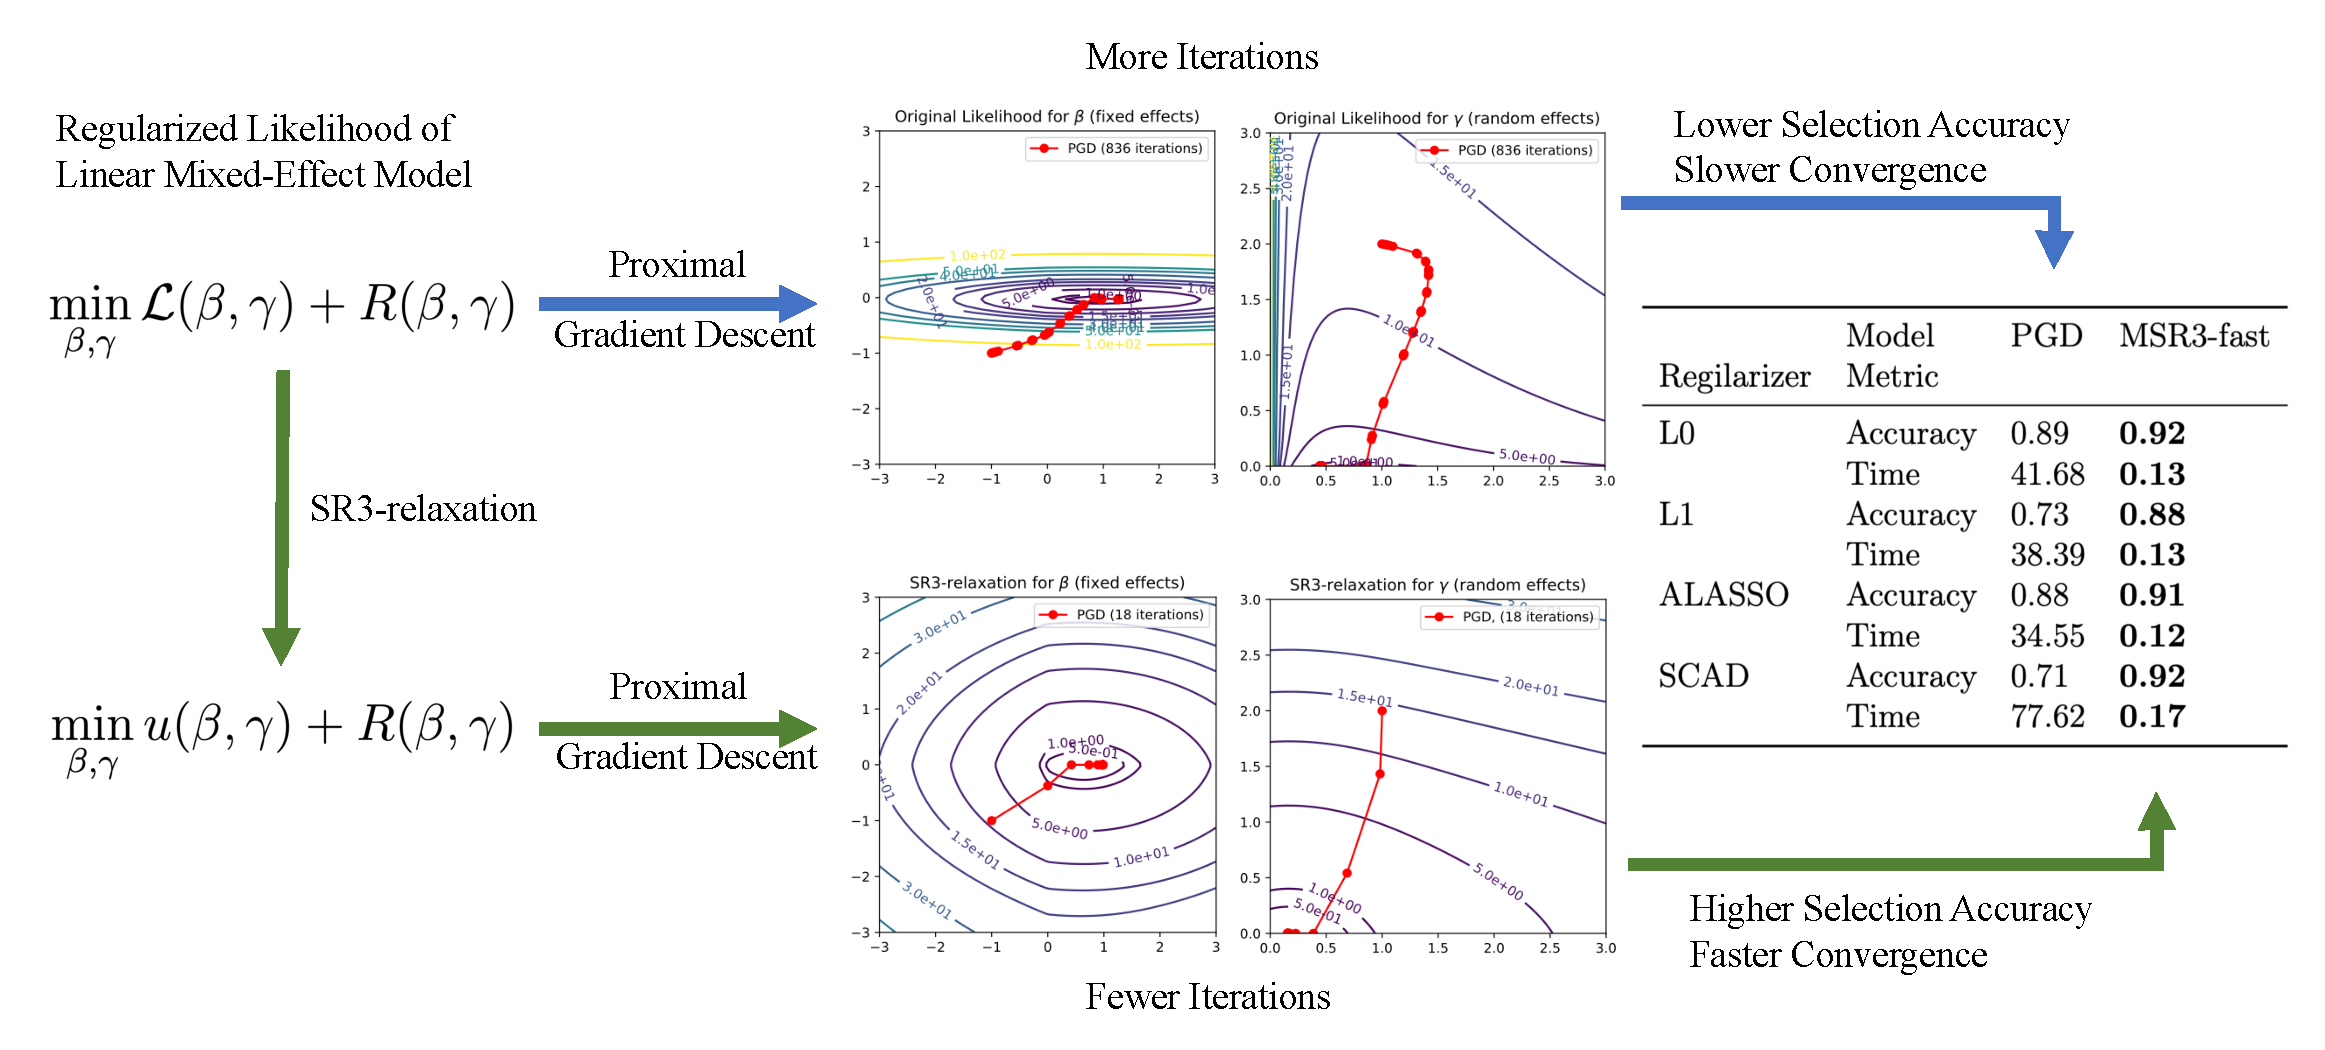
\includegraphics[width=\textwidth]{figures/summary_picture.pdf}
    \caption{Selection of fixed and random effects for LME likelihoods $\mathcal{L}$ using 
    `regularization-agnostic' framework and its SR3 extension using four regularizers. 
    %standard and SR3-relaxed linear mixed-effect likelihoods with popular sparsity-promoting regularizers for the task of simultaneous 
    %The original likelihood $\LL(\beta, \gamma)$ (Eq. \ref{eq:lmm_objective}) is relaxed with SR3 approach to obtain $u(\beta, \gamma)$ (Eq. \ref{eq:value_function_definition}). Both setups are then solved using the same Proximal Gradient Descent (PGD) algorithm. 
    SR3 relaxation accelerates algorithmic converge  (middle panel), and gives better robustness and improved performance on synthetic problems across regularizers (right panel)}.
    \label{fig:summary}
\end{figure}

In this work we develop a regularization-agnostic covariate selection strategy that (1) is fast and simple to implement, (2) provides robust models, and (3) is flexible enough to support most regularizers currently used in variable selection across different domains.  The baseline approach uses the proximal gradient descent (PGD) method, which has been studied by the optimization community for over 40 years, but has not been widely used in LME covariate selection. We provide proximal operators for commonly used regularizers and show how to apply the PGD method to the nonconvex LME setting. In particular we apply the PGD method to four regularizers, 
including the $\ell_0$ regularizer, which does not admit local quadratic approximations and has not been used before for LME variable selection strategies. 

We also develop a new meta-approach that can improve the performance of LME selection methods for any regularizer. Specifically, we extend sparse relaxed regularized regression (SR3) framework~{(\cite{Zheng2019SR3})} to the LME setting. In linear regression, SR3 accelerates and improves the performance of  regularization strategies by introducing auxiliary variables that decouple the accuracy and sparsity requirements for the model coefficients.
We develop a conceptual and algorithmic approach necessary to extend the SR3 concept to LME.  This development is necessary because the LME problem is nonlinear, nonconvex, and includes constraints on variance parameters.  We show that the new approach yields superior results in terms of specificity and sensitivity of feature selection, and is also computationally efficient.  

\edit{Add a paragraph summarizing results from the theory paper}

All new methods are implemented in an open-source library called \texttt{pysr3}, which fills a gap for python mixed-models selection tools in \texttt{Python} (\cite{Buscemi2019Survey}, Table 3). Our algorithms are  1-2 orders of magnitude faster than available LASSO-based libraries for  mixed effects selection in \texttt{R},  see Table \ref{table:glmmlasso}. \texttt{pysr3} enables a standardized comparison of different methods in the LME setting, and makes both the PGD framework and its SR3 extension available to practitioners working with LME models. 

\edit{Extend on the package summary using JOSS paper}

%\subsection{Notation}
%\begin{enumerate}
%\item sets like $\N$, $\B$, $\bS$, $\SS$.
%\item nonsmooth stuff, subdifferential and normal cones
%\end{enumerate}

\section{Linear Mixed-Effects Models: Notation and Fundamentals}
Mixed-effect models describe the relationship between an outcome variable and its predictors when the observations are grouped, for example in studies or clusters.  To set the notation, consider $m$ groups of observations indexed by $i$, with sizes $n_i$, and the total number of observations equal to $n = n_1 + n_2 + \dots + n_m$. For each group, we have design matrices for fixed features $X_i \in \R^{n_i \times p}$,  and matrices of random features $Z_i \in \R^{n_i \times q}$, along with vectors of outcomes $Y_i \in \R^{n_i}$. 
%Typically, columns of $Z_i$ are a subset of columns $X_i$ but it does not have to be the case in general. 
Let 
{$X = [X_1^T, X_2^T, \dots, X_m^T]^T$ and $Z = [Z_1^T, Z_2^T, \dots, Z_m^T]^T$.} 
Following~\cite{Patterson1971, Pinheiro2000}, we define a Linear Mixed-Effects (LME) model as
\eq{
	\label{eq:lme_setup}
	Y_i & = X_i\beta + Z_iu_i + \varepsilon_i, \quad i = 1 \dots m \\
	u_i & \sim \NN(0, \Gamma),\quad \Gamma \in \bS_{+}^{q} \\
	\varepsilon_i & \sim \NN(0, \Lambda_i), \quad \Lambda_i \in \bS_{++}^{n_i}
}
 where $\beta \in \R^p$ is a vector of fixed (mean) covariates, 
 $u_i \in \R^{q}$ are unobservable random effects assumed to be distributed normally with zero mean and the unknown covariance matrix $\Gamma$, and $\bS_{+}^{\nu}$ 
 and $\bS_{++}^{\nu}$ are the sets of
 real symmetric $\nu\times \nu$ positive semi-definite
 and positive definite matrices, respectively. 
Matrices $Z_i$ encode a wide variety of models, including
random intercepts ($Z_i$ are columns of 1's that add $u_i$ to all datapoints from the $i$th study)
and random slopes ($Z_i$ also scale $u_i$ according to the magnitude of a covarite), see e.g.~\cite{pinheiro2006mixed}. 
%In these typical examples, the columns of $Z_i$ are subsets of the columns
%of $X_i$.  
In our study, we assume that the observation error covariance matrices 
$\Lambda_i$ are given and that the random effects covariance matrix 
is an unknown diagonal matrix, i.e., $\Gamma = \Diag{\gamma}, \ \gamma \in \R^s_+$.
% either
% assumed to have a simple parametric form, such as $\Lambda_i=\sig_i I$
% with $\sig_i$ to be determiined, or given given  
 %; we focus on the latter case below. 
 
Defining group-specific error terms $\omega_i = Z_i u_i + \varepsilon_i$, we get a compact formulation that 
recasts~\eqref{eq:lme_setup} as a correlated noise model:
 \eq{
 \label{eq:lmm_correlated_noise_setup}
	Y_i = X_i\beta + \omega_i,\quad \omega_i \sim \NN(0, \Omega_i(\Gamma)), \quad \Omega_i(\Gamma) = Z_i\Gamma Z_i^T + \Lambda_i.
}
For brevity, we refer to $\Omega_i(\Gamma)$ as just $\Omega_i$.
%without the parentheses. In fact, $\Omega_i$ will be the only terms depending on $\Gamma$ in the majority of expressions including the mixed model's likelihood and its derivatives described below.
The reformulation \eqref{eq:lmm_correlated_noise_setup}
yields the following marginalized  negative log-likelihood function of a linear mixed-effects model~\citep{Patterson1971}:
\eq{
	\label{eq:lmm_objective}
	\LL_{ML}(\beta, \Gamma)  :=
%	 \textabove{$\Delta$}{=}
	 \sum_{i = 1}^m \half(y_i - X_i\beta)^T\Omega_i^{-1}(y_i - X_i\beta) + \half\ln{\det{\Omega_i}}.
}
Maximum likelihood estimates for $\beta$ and $\Gam$ are obtained by
solving the optimization problem
\eq{
	\label{eq:ml_lme_optimization_setup}
	\min_{\beta, \Gamma} & \ \LL_{ML}(\beta, \Gamma)  \quad \mbox{s.t.} \quad \ \Gamma \in \bS_{+}^{q}.
}

\begin{theorem}[Existence of a Minimizer, Theorem 1 from \cite{aravkin2022jimtheory}]\label{thm:basic existence}
Let the assumptions in the statement of problem \eqref{eq:ml_lme_optimization_setup} hold. Then optimal solutions to
\eqref{eq:ml_lme_optimization_setup} exist.
\end{theorem}

At this point, we bring in three basic definitions from variational analysis~\cite{rockafellar2009variational}. 

\begin{definition}[Epigraph and level sets]
The epigraph of a function $f:\mathbb{R}^n\rightarrow \mathbb{R} \cup \{\infty\}$ is defined as
\[
\epi f = \{(x,\alpha) : f(x) \leq \alpha\}. 
\]
For a given $\alpha$, the $\alpha$-level set of $f$ is defined as
\[
\text{lev}_\alpha f = \{x: f(x) \leq \alpha\}.
\] 
\end{definition}

\begin{definition}[Lower semicontinuity and level-boundedness]
A function $f:\mathbb{R}^n\rightarrow \mathbb{R} \cup \{\infty\}$ is lower semicontinous (lsc) when $\epi f$ is closed, 
and level-bounded when all level sets $\text{lev}_\alpha f$ are bounded.  
\end{definition}


\begin{definition}[Convexity]
A function $f:\mathbb{R}^n\rightarrow \mathbb{R} \cup \{\infty\}$ is convex when $\epi f$ is a convex set. Equivalently, 
\[
f(\lambda x + (1-\lambda)y) \leq \lambda f(x) + (1-\lambda) f(y) \quad \forall x,y\in\dom{f},\ \lambda \in (0,1),
\]
where $\dom{f}:=\lset{x\in\Rn}{f(x)<+\infty}$.
\end{definition}

\begin{definition}[Weak convexity]
A function $f:\mathbb{R}^n\rightarrow \mathbb{R} \cup \{\infty\}$ is $\eta$-weakly convex 
$f(\cdot)+\frac{\eta}{2}\|\cdot\|^2$ is convex. 
\end{definition}

The negative log likelihood~\eqref{eq:ml_lme_optimization_setup}  is nonlinear and nonconvex, and requires an iterative numerical solver.
However, it is convex with respect to $\beta$, and weakly convex with respect to $\gamma$, with a weak convexity constant $\overline \eta$
computed in~\cite[Section 5.1]{Theory1} . The expected value of the posterior mode $\beta$ given $\Gamma$ has the closed form representation 
%\eq{
%	
\[
\label{eq:beta_formula}
	\beta(\Gamma) = \argmin_{\beta}\LL(\beta, \Gamma) = \left(\sum_{i = 1}^m X_i^T\Omega_i^{-1}X_i\right)^{-1}\sum_{i = 1}^mX_i^T\Omega_i^{-1}y_i.
\] %}
By using the simplification $\Gam=\Diag{\gam}$, we obtain the problem
%{In the meta-analysis setting under study, 
%In our study, we assume that $\Gam$ is a diagonal matrix of the form
%$\Gamma = \Diag{\gamma}, \ \gamma \in \R^s$ with the 
%$\Lambda_i \in \R_{++}^{n_i \times n_i}$ fixed and given 
%%the positive definite constraint from (\ref{eq:ml_lme_optimization_setup}) transforms into a box constraint:
%so that our problem takes the form}
\eq{
	\label{eq:lme_diagonal_setup}
	\min_{\beta\in\R^p, \gam\in\R^q_+} & \ \LL(\beta,\gam)
	:=\LL_{ML}(\beta, \Diag{\gamma}) 
%	\\
%	s.t. & \ \gamma \geq 0\ .
	}
%Under the assumption $\Lambda_i \in \R_{++}^{n_i \times n_i}$ in~\eqref{eq:lme_setup}, 
In this setting, when an
entry $\gamma_j$ takes the  value $0$ the corresponding coordinates of all random effects $u_{ij}$ are identically $0$ for all $i$. 

Verification of the existence to solutions to \eqref{eq:lme_diagonal_setup}
and, more generally, \eqref{eq:ml_lme_optimization_setup} follows from the work of \cite{zheng2021trimmed}.
Standalone proofs for the existence of minimizers are developed in~\cite[Theorem 1]{Theory1},
and extended to the presence of regularizers in~\cite[Theorem 2]{Theory1}. %, restated below for convenience. 


%%Here we streamline these techniques and extend to the regularized case, 
%%with basic results given below, with proofs in the appendix.  
%
%\begin{theorem}[Existence of a Minimizer]\label{thm:basic existence}
%Let the assumptions in the statement of problem \eqref{eq:ml_lme_optimization_setup} hold. Then optimal solutions to
%\eqref{eq:ml_lme_optimization_setup} exist.
%\end{theorem}
%
%Feature selection methods  include sparsity-inducing penalties or constraints. See~\cite[Theorem 1]{Theory1}
%for an existence result under weak assumptions on the regularizer. 
%
%
% 
%
%\begin{theorem}\label{thm:basic existence2}
%Let the assumptions in the statement of problem \eqref{eq:lme_diagonal_setup} hold,
%define $\LL(\beta,\gam):=\LL_{ML}(\beta, \Diag{\gamma})$
%and suppose $\map{\hR}{\R^p\times\R^q_+}{\R\cup\{+\infty\}}$ 
%is lsc and level bounded.
%Then $\LL+\hR$ is level bounded and solutions to
%the following optimization problem exist:
%\eq{
%\label{eq:extended loss}
%\min_{\beta\in\R^p, \gamma\in\R^q_+}  \LL(\beta, \gamma) + 
%\hR(\beta, \gamma) .
%}
%\end{theorem}

%\red{I don't get the point of the following paragraph. Indeed, it seems wrong.}

This paper focuses the case where $\Gamma$ is diagonal, 
  (often referred to as \textit{the diagonal setup}) 
 and all $\Lambda_i$ are known (see \eqref{eq:lme_diagonal_setup}), 
following the meta-analysis use-case~\citep{zheng2021trimmed} that is widely used in epidemiological studies~\cite{murray2020global}. 
While the proposed approach can be extended to the non-diagonal case, we leave it for future work, save for a brief discussion in Section~\ref{sec:applications}.

\subsection{Prior Work on Feature Selection for Mixed-Effects Models}
\label{sec:prior_work}

Variable (feature) selection models seeks to select or rank the most important predictors in a dataset in order to get a parsimonious model at a minimal cost to prediction quality. 
%The selection process often occurs simultaneously with fitting the model, and a predictor is `selected' if its respective coefficient in the model is non-zero. 
If the desired number of coefficients $k$ is given, then the feature selection problem can be formulated as the minimization of a loss function $f(\theta)$ (e.g. the negative log-likelihood) subject to a zero-norm constraint:
\eq{
	\label{eq:general_feature_selection_zero_norm}
	&\min_{\theta}  f(\theta) \quad \mbox{ s.t. }  \quad \|\theta\|_0 \leq k 
	}
where $\|\theta\|_0$ denotes the number of nonzero entries in $\theta$, see panel (c) of Figure~\ref{fig:regularizers}.

%\begin{figure}
%    \centering
%    \begin{tabular}{cc}
%    \includegraphics[width=0.3\textwidth]{figs/l0_regularizer.pdf}
%    &
%        \includegraphics[width=0.3\textwidth]{figs/l1_regularizer.pdf}\\
%        (a) $\ell_0$ & (b) $\ell_1$ \\
%           \includegraphics[width=0.3\textwidth]{figs/lh_regularizer.pdf}
%    &
%        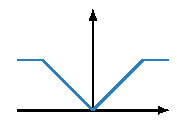
\includegraphics[width=0.3\textwidth]{figs/scad_regularizer.pdf}\\
%              (a) $\ell_{1/2}$ & (b) Clipped Absolute Deviation (CAD) 
%    \end{tabular}
%    \caption{Common convex and non-convex regularizers used for feature selection.}
%    \label{fig:regularizers}
%\end{figure}


% In this form the problem is equivalent to the Knapsack problem, which is NP-complete. Many techniques based on exhaustive search, also known as subset selection process, were developed, and showed to be effective when the total number of predictors is small (see \cite{Muller2013}). The same setup appears to be intractable in a high-dimension setting due to the exponential growth of the number of subsets to check when $n \to \infty$, however, it's possible to get an approximate solution via relaxation techniques.

 \begin{figure}[ht]
    \centering
    \begin{tabular}{ccc}
        \includegraphics[width=0.3\textwidth]{figures/l1_regularizer.pdf}
&
           \includegraphics[width=0.3\textwidth]{figures/lh_regularizer.pdf}
    &
    \includegraphics[width=0.3\textwidth]{figures/l0_regularizer.pdf}\\
  %      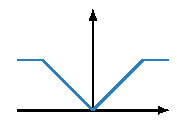
\includegraphics[width=0.3\textwidth]{figs/scad_regularizer.pdf}\\
              (a) $\ell_1$  & (b) $\ell_{1/2}$ & (c) $\ell_0$
    \end{tabular}
    \caption{Common convex and non-convex regularizers used for feature selection.}
    \label{fig:regularizers}
\end{figure}


The constraint in \eqref{eq:general_feature_selection_zero_norm} is 
combinatorial, and a common workaround is to relax it to a one-norm constraint, 
with $\|\theta\|_1$ equal to the sum of absolute values of the entries of $\theta$. 
The best-known example of this approach is the least absolute square shrinkage operator (LASSO) studied by \cite{Tibshirani1996} for linear regression, 
see panel (a) of Figure~\ref{fig:regularizers}.
% for the least squares model:
% \eq{
% 	\label{eq:lasso_regression}
% 	\min_\theta f(\theta) + \lambda||\theta||_1
 %
 
% LASSO combines the small bias of the least-square estimator and the interpretability of the subset selection method, producing
% %, however, 
% biased estimates for the large coefficients~\citep{Zou2006}.  This approach has been extended to leverage many other regularizers that exhibit useful properties including bias 
%reduction for larger coefficients (SCAD from \cite{Fan2001}), simultaneous selection for highly correlated predictors (Elastic Net from \cite{Zou2005}), or better selection accuracy using non-penalized solution's coordinates as weights (A-LASSO from \cite{Zou2006}).
  
 Feature selection for LMEs is more difficult than for linear regression models. 
 In linear regression the observations are independent, whereas in mixed-effects setup they are generally correlated. 
 In addition, LMEs have both mean effect variables  $\beta$ as well as random variance variables 
 $\Gamma$. % where the groups can have different relative importance. 
% Finally, selecting random features implies that $\Gamma$ will have zero columns and rows thereby forcing the optimization methods to the boundary of the feasible parameter set and making both the theoretical analysis and numerical computations more challenging.  
The shrinkage operator approach for linear regression 
\citep{Tibshirani1996} was first adapted 
to the problem of feature selection for the fixed effects in mixed-effect models by \cite{Lan2006}. 
The removal of a random effect from the model requires the elimination of an entire row and column from $\Gamma$. 
To make the problem more tractable, \cite{Chen2003} reparamtrized $\Gamma$ through a modified Cholesky decomposition $\Gamma(D,L): = DLL^TD$, where $D$ is a diagonal matrix and $L$ is a lower-triangular matrix with ones on the main diagonal, and focused on selecting elements of $D$. 
% In this case, one can select variance parameters by selecting the elements of the diagonal matrix $D$ while treating the non-diagonal entries of $L$ as free parameters. 
Based on this idea, \cite{Krishna2008} extended the Adaptive LASSO regularizer (\cite{Lan2006, Xu2015}) to mixed-effects setting using the objective
   \[
        \LL(\beta, \Gamma(D,L)) + \lambda\left(\sum_{i = 1}^p 
        \left|\frac{\beta_i}{\hat\beta_i}\right| + \sum_{j = 1}^q \frac{D_{ii}}{\hat{D_{ii}}} \right),
   \]
 where $\hat\beta$ and $\hat{D}$ are the solution of a non-penalized maximum likelihood problem and $\lambda$ is a tuning parameter for the weighted regularizer
 and is called the regularization parameter. 
 %This strategy has a well known issue: non-penalized estimates $\hat\beta$ and $\hat{D}$ may be inaccessible because the numerical algorithm may fail to converge, especially when the underlying solution is sparse. 
 \cite{Ibrahim2011} use a similar approach, penalizing  non-zero elements $\Gamma_{ij}$ directly. 
 Other methods that use Adaptive LASSO for simultaneous selection 
 of fixed and random effects are \cite{Lin2013, fan2014robust, pan2018simultaneous}. Adaptive LASSO is available to practitioners via \texttt{R} packages \texttt{glmmLasso}\footnote{\href{https://rdrr.io/cran/glmmLasso/man/glmmLasso.html}{https://rdrr.io/cran/glmmLasso/man/glmmLasso.html}} (\cite{groll2014variable}) and \texttt{lmmLasso}\footnote{\href{https://rdrr.io/cran/lmmlasso/}{https://rdrr.io/cran/lmmlasso/}}(\cite{schelldorfer2011estimation}).

 A popular nonconvex regularizer used for feature selection is smoothed clipped absolute deviation (SCAD)~\cite{Fan2001}. 
 %The (non-smoothed) clipped absolute deviation penalty is depicted in panel (d) of Figure~\ref{fig:regularizers}.
% , and the algebraic forms for both CAD and SCAD are given in the appendix. 
% which acts on the first derivative of the penalty function $p_\lambda(\theta)$:
 %  \eq{
  % 		p'_{\lambda}(|\theta|) = \lambda\left\{\ind{\theta \leq \lambda} +  \frac{(a\lambda - \theta)_+}{(a-1)\lambda}\ind{\theta - \lambda} \right\}
  % }
The adaptation of the SCAD penalty to select both fixed and random features in 
linear mixed models was developed by \cite{Fan2012}. SCAD was also used by \cite{chen2015inference} for selecting fixed effects and establishing the existence of random effects in ANOVA-type models. Finally, \cite{Ghosh2018} studied SCAD regularization for selecting mean effects in high-dimensional genomics problems.

\edit{Add more methods for feature selection \cite{Buscemi2019Survey, Muller2013}}

To better compare methods, we need to consider the regularization parameter 
\plum{$\lambda$} and how it is tuned. 
The output of a shrinkage model critically depends on the tuning parameter 
$\lambda$. The entire range of possible $\lambda$ values is captured 
by the notion of a ``$\lambda$-path in the model space'', with  the best parameter and the final model chosen using information criteria. According to \cite{Muller2013}, the most widely used information criterion is the marginal AIC criterion (\cite{Vaida2005}):
  \eq{
  \label{eq:vaida_aic}
  AIC := 2\LL(\hat{\theta}) + 2\alpha_n(p+q)
  }
  where $\hat\theta$ includes all the estimated parameters $(\beta, \Gamma)$, and $\alpha_n := n(n-p-q-1)$ for the finite sample case (\cite{Sugiura1978}). 
  %As discussed by \cite{Fang2011}, AIC is asymptotically equivalent to leave-one-out cross-validation, so it can be used for choosing between a finite number of models. AIC, however, is also known to be positively-biased (\cite{Ibrahim2011}). 
  Alternatively, LASSO-type methods (\cite{Krishna2008, Ibrahim2011}) use a BIC-type information criterion:
  \eq{
    BIC := 2\LL(\hat{\theta}) + \log(n)(p+q).
  }
BIC performs well in practice, but does not have theoretical guarantees~(\cite{schelldorfer2011estimation}).
  %One can refer to \cite{Muller2013, Buscemi2019Survey} for a detailed overview of different feature selection approaches.
  
\edit{Add more ICs (e.g. Muller)}
  
\section{Algorithms for Feature Selection}
\label{sec:pgd_methods}
We approach feature selection by adding a regularizer to model \eqref{eq:lme_diagonal_setup}: 
%( $\Lam_i$ are known and given, and $\Gamma$ an unknown diagonal matrix,   
%to be estimated along with the fixed effects $\beta$. 
%and add a regularizer:
%to the objective to obtain the optimization problem described
%in Theorem \ref{thm:basic existence2}:

%Feature selection is imposed by adding
%Consider a mixed-effect model setting described in Eq. (\ref{eq:lme_setup}) with $\Gamma$ being diagonal: $\Gamma = \Diag{\gamma}$.  
%We wish to find a minimizer of the problem 
%\eq{
%	\label{eq:lme_loss_original}
%	\min_{\beta\in\R^p, \gamma\in\R^q_+} & \LL(\beta, \gamma) + R(\beta, \gamma), 
%	}
\eq{%\label{eq:main opt in x over C}
    \label{eq:lme_loss_original_in_x}
    \min_{x } & \LL(x) + R(x)+ \delta_{\CC}(x),
%    \\
%    \text{s.t. } & x \in \CC\ .
}
where $x = (\beta, \gamma)$, 
$\CC:=\R^p\times \R^q_+$,
$\map{R}{\R^P\times\R^q_+}{\eR_+:=\R_+\cup\{+\infty\}}$
is a 
lower semi-continuous (lsc) regularization term, and
$\delta_{\CC}$ is the convex indicator function
\[
    \delta_{\CC}(x) := \begin{cases} 0, &  x \in \CC \\ +\infty, & x \not\in \CC .\end{cases}
\]  
By \cite[Theorem 2]{Theory1}, solutions to \eqref{eq:lme_loss_original_in_x}
always exist when $R$ has compact lower level sets.
% or 
% $\LL(\beta, \gamma)=\LL_{REML}(\beta,\Diag(\gamma))$ in \eqref{eq:reml_objective} with 
% \[
% \B=[\zero,\gam_\mmax\one]:=\left\{ \gamma\, |\, 0\le \gamma_i\le \gam_\mmax,\ i=1,\dots,q\right\}
% \]
% for some $\gam_\mmax>0$ where $\one$ is the vector of the appropriate
% dimension each of whose components is one.
% Since the method applies to either likelihood, hereafter we omit the subscripts and use $\LL$ to denote the objective function. %, leaving this choice up to a practitioner.
%For conciseness, define $x = (\beta, \gamma)$ and 
%$\CC:=\R^p\times \R^q_+$.
%such that $\tbeta \in \R^p$ is unconstrained and $\tgamma \in \R^q_+$ is non-negative:
%\eq{
% x\in \CC \textabove{$\Delta$}{=} \{[\beta', \gamma']: \  \beta' \in \R^p, \ \gamma' \in \R^q_+\} \subset \R^{p+q} 
%}
%With this notation, problem \eqref{eq:lme_loss_original} becomes
%\eq{%\label{eq:main opt in x over C}
%    \label{eq:lme_loss_original_in_x}
%    \min_{x \in \CC} & \LL(x) + R(x),
%    \\
%    \text{s.t. } & x \in \CC\ .
%}
%Equivalently, the box constraint can be moved to the loss in a form of an indicator function:
%or equivalently
%\[
%\eq{
%	\label{eq:lme_loss_original}
%    \min_{x} \LL(x) + R(x) + \delta_{\CC}(x)\ ,
%}
%where 
%$x = (\beta, \gamma)$, 
%$\CC:=\R^p\times \R^q_+$,  
%\quad \text{where}\ \, 
%\delta_{\CC}$ is the convex indicator function
%\[
%    \delta_{\CC}(x) := \begin{cases} 0, &  x \in \CC \\ +\infty, & x \not\in \CC .\end{cases}
%\]
The most common regularizers are separable taking the form
\begin{equation}\label{eq:R sep}
R(x) = \sum_{i = 1}^p r_i(x_i), 
\end{equation}
with typical choices for the component functions $r_i$ given in Table \ref{table:proxes}.


\subsection{Variable Selection via Proximal Gradient Descent}

Since $\LL$ is differentiable on its domain and 
proximal operator
for $\alpha R + \delta_{\CC}$ is 
computationally tractable, 
the Proximal Gradient Descent (PGD) Algorithm (e.g. see \cite{AB17}) offers a simple numerical
strategy for estimating first-order stationary points for 
\eqref{eq:lme_loss_original_in_x}.
% when 
%the application of the . 
%
%whenever the application of the proximal operator \cite{}
%to $\alpha R + \delta_{\CC}$ is 
%computationally tractable, a simple numerical method for estimating
%first-order stationary points for \eqref{eq:lme_loss_original_in_x} is
%the Proximal Gradient Descent (PGD) Algorithm. 
The proximal operator for 
$\alpha R + \delta_{\CC}$ is defined as the mapping
\[ %\eq{
    \prox_{\alpha R + \delta_{\CC}}(z) := \argmin_{y\in \CC}\ R(y) + \frac{1}{2\alpha}\|y - z\|_2^2 ,
\] %}
and the PGD iteration is given by
\[
    x^+ = \prox_{\alpha R + \delta_{\CC}}(x - \alpha \nabla \LL(x)),
\]
where $\alpha$ is a stepsize.
When $R(x)$ has the form given in \eqref{eq:R sep}, we have
\[
 \prox_{R}(z) = (\prox_r(z_1), \dots, \prox_r(z_q)) .
\]
\begin{table}[H]
\small
    \centering
    \begin{tabular}{|p{25.4mm}|c|c|}
        \hline
         \!\!Regularizer & $r(x)$, $x \in \R$ & $\prox_{\alpha r}(z)  $ \\
         \hline \hline
         LASSO ($\ell_1$) \newline (\cite{tibshirani1996regression}) & $|x|$ & $\sign(z)(|z| - \alpha)_+$ \\
         \hline
         A-LASSO \newline (\cite{Fan2001}) & $\bar{w}|x|$, $\bar{w} \geq 0$ &  $\sign(z)(|z| - \alpha\bar{w})_+$\\
         \hline
         SCAD \newline (\cite{fan1997comments}) & $\begin{cases} \sigma |x|, & |x| \leq \sigma \\ \frac{-x^2 + 2\rho\sigma x - \sigma^2}{2(\rho - 1)}, & \sigma < |x| < \rho\sigma \\ \frac{\sigma^2(\rho + 1)}{2}, & |x| > \rho\sigma \end{cases}$ & $\begin{cases} \sign(z)(|z| - \sigma\alpha)_+, & |z| \leq \sigma(1+\alpha) \\ \frac{(\rho - 1)z - \sign(z)\rho \sigma\alpha}{\rho - 1 - \alpha}, & \sigma(1+\alpha) < |z| \\
         &\quad\leq \max(\rho, 1+\alpha)\sigma \\ z, & |z| > \max(\rho,1+\alpha)\sigma \end{cases}$ \\
%         \hline
%         $\ell_p$, $0 < p < 1$ & $|x|^p$ & Coordinate Newton (\cite{Zheng2019SR3}) \\
         \hline
         $\delta_{\|x\|_0 \leq k}$  \newline ($\ell_0$ ball) & $\begin{cases} 0, & \#\{|x_i| \neq 0\} \leq k\\ \infty, & \text{ otherwise}\end{cases}$ & keep $k$ largest $|x_i|$, set the rest to 0 \\
         \hline
    \end{tabular}
    \caption{Proximal operators for commonly used sparsity-promoting regularizers. }
    \label{table:proxes}
\end{table}

\edit{Make section "Evaluating proximal operators" using Appendix}

Under the assumption that $R$ is level-compact \cite{aravkin2022jimtheory} extended Theorem \ref{thm:basic existence} to the regularized case as follows:

\begin{theorem}[Existence of a Minimizer for \ref{eq:lme_loss_original_in_x}, \cite{aravkin2022jimtheory}, Theorem 2]

\label{thm:basic existence2}
Let the assumptions in the statement of problem \eqref{eq:lme_diagonal_setup} hold.
%define $\LL(\beta,\gam):=\LL_{ML}(\beta, \Diag{\gamma})$
Suppose $\map{\hR}{\R^p\times\R^q_+}{\R\cup\{+\infty\}}$ 
is lsc and level compact (i.e., $\epi{R}:=\lset{(\bg,\nu)}{R\bg\le\nu}$ is closed
and $\lset{\bg}{R\bg\le\nu}$ is bounded for all $\nu\in\R$).
Then $\LL+\hR$ is level compact and solutions to
the following optimization problem exist:
\eq{
\label{eq:extended loss}
\min_{\beta\in\R^p, \gamma\in\R^q_+}  \LL(\beta, \gamma) + 
\hR(\beta, \gamma) .
}
\end{theorem}

In practice, it is often advisable to include a constraint of the form 
$\gamma\le\gammax$ for $\gam\in\R^q_{++}$ chosen
sufficiently large since an excessively large variance usually indicates 
that the model is poorly posed and needs review. 
Such a constraint is also numerically expedient since it prevents $\gam$ from diverging. Table \ref{table:proxes} provides closed form expressions for the proximal operators 
of commonly used regularizers. 
%All regularizers in this list are separable except $R(x) = \delta_{\|x\|_0 \leq k}$, for which the solution also has an analytically closed form.
%Again when $R$ is separable with the $r_i$ coming from Table \ref{table:proxes}, 
%the evaluation of 
For all of these cases,  the following theorem gives closed form expressions for
$\prox_{\alpha R + \delta_{\CC}}(z)$.

\begin{theorem}[Proximal operator for bounded $\gamma$]     \label{thm:prox_of_positive_quadrant}
We consider modified regularizers $r(\gamma)$ from the Table \ref{table:proxes} 
% and let $v = (\beta, \gamma)$. % \in \CC \subset R^{p + q}$.
that include an additional constraint on $\gamma$ of the form 
\[
0 \leq \gamma \leq \bar\gamma,
\]
for $\bar\gamma\in[0,+\infty]$.
%which which the positive orthant as a special case (i.e. $\bar\gamma = \infty$). 
We have the following results. 
%    \begin{enumerate}
%    \item  For $R(x)$ given by LASSO, A-LASSO, CAD, and SCAD, we have  for all $i$ that 
    %\eq{
    %\prox_{\alpha R + \delta_{\CC}}(v) = (\prox_{\alpha r}(v_1), \dots, \prox_{\alpha r}(v_p), \prox_{\alpha r + \delta_{\R_+}}(v_{p+1}), \dots, \prox_{\alpha r + \delta_{\R_+}}(v_{p+q}))
    %}
    %where 
 %   \eq{
 %   \prox_{\alpha r + \delta_{\R_+}}(v_{i}) = \begin{cases} \prox_{\alpha r}(v_i), & v_i \geq 0 \\ 0, & \text{ otherwise} \end{cases} 
%    \item For $R(x) = \delta_{\|x\|_0 \leq k}$, the $\prox_{\alpha R + \delta_{\CC}}(v)$ can be evaluated by taking $k$ largest non-negative coordinates of $v$, and setting the rest to $0$.
 %   \end{enumerate}
%    Next, suppose $\LL = \LL_{REML}$. 
    \begin{enumerate}
    \item  For SCAD, we have for all $i$ that  
   % \eq{
%    \prox_{\alpha R + \delta_{\CC}}(v) = (\prox_{\alpha r}(v_1), \dots, \prox_{\alpha r}(v_p), \prox_{\alpha r + \delta_{\R_+} + \delta_{\R_{\leq \bar\gamma}}}(v_{p+1}), \dots, \prox_{\alpha r + \delta_{\R_+} + \delta_{\R_{\leq \bar\gamma}}}(v_{p+q}))
 %   }
  %  where 
%    \eq{
\[
    \prox_{(\alpha r + \del_{[0,\bgam]})} %\delta_{\R_+} + \delta_{\R_{\leq \bar\gamma}}}
    (\gamma_{i}) = \begin{cases} 
        \prox_{\alpha r}(\gamma_i), & 0 \leq \gamma_i < \bar\gamma  \\
        \bar\gamma, & \gamma_i \geq \bar\gamma \\
        0, & \text{ otherwise} \end{cases}
\]
%    }
    \item  For LASSO, A-LASSO we have for all $i$ that 
 %   \eq{
  %  \prox_{\alpha R + \delta_{\CC}}(v) = (\prox_{\alpha r}(v_1), \dots, \prox_{\alpha r}(v_p), \prox_{\alpha r + \delta_{\R_+} + \delta_{\R_{\leq \bar\gamma}}}(v_{p+1}), \dots, \prox_{\alpha r + \delta_{\R_+} + \delta_{\R_{\leq \bar\gamma}}}(v_{p+q}))
  %  }
  %  where 
%    \eq{
\[
\prox_{(\alpha r + \del_{[0,\bgam]})}(\gamma_i) 
%    \prox_{\alpha r + \delta_{\R_+} + \delta_{\R_{\leq \bar\gamma}}}(v_{i}) 
    = \begin{cases} 
        \prox_{\alpha r}(\gamma_i), & 0 \leq \gamma_i < \bar\gamma + \alpha \\
        \bar\gamma, & \gamma_i \geq \bar\gamma + \alpha \\
        0, & \text{ otherwise} \end{cases}
\]
%    }
    \item For $R(\cdot) = \delta_{\lev{\norm{\cdot}_0}{k}}$  %\delta_{\|x\|_0 \leq k}$, 
    the $\prox_{\alpha R + \delta_{\CC}}(\gamma)$ can be evaluated by taking $k$ largest coordinates of $\gamma$ such that $0 \leq \gamma_i \leq \bar\gamma$, and setting the 
    remainder to $0$.
    \end{enumerate}
\end{theorem}
The proof of the Theorem \ref{thm:prox_of_positive_quadrant} is provided in Appendix \ref{appendix:proxes}. 
%\textcolor{red}{Aleksei, please check proof of appendix is all in terms of $\gamma$, rather than $v = (\beta, \gamma)$.}
The  PGD algorithm is detailed in Algorithm~\ref{alg:pgd_for_lme}.
{The algorithm's step-size $\alpha$ depends on the Lipschitz constant; an upper-bound is given in Appendix \ref{appendix:lipschitz_constant}. In practice, $\alpha$ is computed using a line-search, since the available estimate for $L$ is very conservative.}

\smallskip

\begin{algorithm}[H]
\SetAlgoLined
$x = x_0$, $\alpha < \frac{1}{L}$,\text{ where } $\LL$ \text{ is $L$-Lipschitz}\\
 \While{not converged}{
    $x^+ = \prox_{\alpha R + \delta_{\CC}}(x - \alpha \nabla \LL(x))$;\\
 }
 \caption{\label{alg:pgd_for_lme}Proximal Gradient Descent for Linear Mixed-Effect Models}
\end{algorithm}
\medskip

\noindent

The main advantages of Algorithm \ref{alg:pgd_for_lme} are its simplicity and flexibility.
The main loop needs only the gradient and prox operator, and the structure of the algorithm is independent of the choice of regularizer $R$.
Algorithm \ref{alg:pgd_for_lme} locates first-order stationary points
under weak assumptions, in particular neither the objective nor the regularizer need to be convex~\citep{AB17,attouch2013convergence}. 

%we use it only as 
%a point of reference for the algorithm that is the focus of our study which is presented in
%the Section \ref{sec:sr3_adaptation_to_lme}.
%The interested reader should consult the \textcolor{blue}{references \cite{} for the 
%various possible convergence properties
%of Algorithm \ref{alg:pgd_for_lme}}.

\edit{Add other optimization methods for FS in LMEs (e.g. Newton)}

\search{Add table of cross-references between optimization methods and regularizers}

\search{Add table with rates of convergence wherever possible}

\begin{figure}[ht]
    \centering
    \includegraphics[width=\textwidth]{figures/intuition_current.pdf}
    \caption{Proximal Gradient Descent (PGD) for~\eqref{eq:value_function_optimization} converges far faster than for~\eqref{eq:lme_loss_original_in_x}, because the SR3-value function $u_\eta$ yields more spherical level-sets than original likelihood for both convex components $\beta$ (first row) and non-convex components $\gamma$ (second row). 
    %The effect is particularly strong for $\gamma$-minimizers near the boundary of the constraint region (bottom-left panel).
    }
    \label{fig:geometric_intuition_sr3}
\end{figure}

\subsection{Variable Selection via MSR3}

To develop an approach that is both more efficient and accurate, we extend the SR3 regularization of~\cite{Zheng2019SR3} to LMEs. 
We call the extension MSR3, since we are focusing on mixed effects models. 
Starting with the regularized likelihood~\eqref{eq:lme_loss_original_in_x} we introduce auxiliary parameters designed to discover the 
fixed and random features: 
\eq{%\label{eq:main opt in x over C}
    \label{eq:lme_loss_sr3}
    \min_{x, w} & \LL(x) + R(w)+ \delta_{\CC}(x) + \kappa_{\eta}(x-w),
%    \\
%    \text{s.t. } & x \in \CC\ .
}
where $\kappa_\eta$ penalizes deviations between $x$ and $w$, and also guarantees that the objective is convex with respect to the $\gamma$
components of $x$ for sufficiently large $\eta$:
\begin{equation}
\label{eq:kappa}
\kappa_{\eta} (\beta, \gamma) = \frac{\eta}{2}\|(\beta,\gamma)\|^2 ,
\end{equation}
with $\eta\ge\bar\eta$ where $\bar \eta$ is the weak convexity constant
computed in~\cite[Section 5.1]{Theory1}.
As $\eta \uparrow \infty$, the extended objective~\eqref{eq:lme_loss_sr3} converges in an epigraphical sense to the original objective~\eqref{eq:lme_loss_original_in_x}. 
However, feature selection accuracy does not require this continuation, and a fixed 
modest value can be used~\citep{Zheng2019SR3}, e.g. $\eta=1$.

To understand the algorithm and logic behind the objective~\eqref{eq:lme_loss_sr3}, we, for this section alone, define a simplified version of the value function $u_\eta(w)$ and the solution set $S_\eta(w)$:
\eq{
	\label{eq:value_function_definition_only_eta}
		u_\eta(w) & = \min_x \ \LL(x) + \delta_{\CC}(x) + \kappa_{\eta}(x-w)\\
		S_\eta(w) & = \argmin_x \LL(x) + \delta_{\CC}(x) + \kappa_{\eta}(x-w).
}
Substituting the above into (\ref{eq:lme_loss_sr3}) the problem transforms into the problem of optimizing a regularized value function:
\eq{
	\label{eq:value_function_optimization}
	\min_{w} u_\eta(w) + R(w)
}
%Thus at a conceptual level, 
Here we have transformed the original regularized likelihood~\eqref{eq:lme_loss_original_in_x}  %has been transformed 
through relaxation and partial 
minimization to obtain an equivalent problem~\eqref{eq:value_function_optimization} 
for $w$ with the same regularizer. The value function $u_\eta$ encapsulates 
global variational information on the function $\LL(x) + \delta_{\CC}(x)$
relative to $w$.
%Problem~\eqref{eq:value_function_optimization} 
%attempts to find sparse $w$ that are small with respect to $u_\eta$. 

In the case of linear regression, 
the function $u_\eta$ has a closed form solution~\cite{Zheng2019SR3}. However, in both  the linear regression context of~\cite{Zheng2019SR3} 
and in the LME context studied here, we need only compute $S_\eta(w)$ 
in order to optimize~\eqref{eq:value_function_optimization}. 
Indeed, in \cite[Section 5]{Theory1} it is shown that $u_\gamma$ is well-defined, 
differentiable, and Lipschitz continuous, with
%and we have a closed form solution for the derivative: 
\begin{equation}\label{eq:grad_value_function_explicit}
\nabla u_\eta(w) = \nabla_w k_\eta(x-w)|_{x = S_\eta(w)}=\eta(w-S_\eta(w)) .  
\end{equation}
%where $\nabla_w k_\eta(x-w)$ is computed directly from~\eqref{eq:kappa}. 

Our empirical studies indicate that 
(\ref{eq:value_function_optimization}) has advantages over (\ref{eq:lme_loss_original_in_x})
from an optimization perspective since $u_\eta(w)$ typically has nearly spherical level-sets while keeping the position of minima close to those of $\LL(x)$. This effect is extensively studied and validated for a quadratic loss function in the original work  of \cite{Zheng2019SR3}. 
%we provide empirical evidence that suggests that it also extends to more general non-linear functions, specifically to the marginal likelihood. 
In Figure \ref{fig:geometric_intuition_sr3}, we plot the level-sets of $\LL(x) + \|x\|_1$ (left column) and $u(w) + \|w\|_1$ (right column) for the same mixed-effect problem. 
%A more symmetrical 
The more spherical geometry of the latter allows the Algorithm \ref{alg:pgd_for_value} 
(described below) to converge in 21 iterations, whereas Algorithm \ref{alg:pgd_for_lme} takes 1284 iterations. The difference is most pronounced when the minimum sits on the boundary of the feasible set, which is always the case for the variable selection problems with sparse support.
%In effect, Algorithm \ref{alg:pgd_for_value} incorporates global variational information 
%about the function $\LL$ while Algorithm \ref{alg:pgd_for_lme}

%The value function $u_\eta(w)$ possesses the following properties: 
%
%\begin{theorem}[Properties of value function optimization]
%\label{thm:properties_of_value_function}
%Let $\eta > 0$, $R(x)$ is level-compact. Then
%\begin{enumerate}
%	\item The solutions for (\ref{eq:value_function_optimization}) always exists when $R(w)$ is level-compact \cite[Theorem 6]{jimtheory}.
%	\item The solution set $S_\eta(w)$ is well-defined, single-valued and continuous \cite[Theorem 9]{jimtheory}
%	\item $u_\eta(w)$ is well-defined and continuous \cite[Theorem 9]{jimtheory}.
%	\item $u_\eta(w)$ is differentiable with $\nabla_w u_\eta(w) = \nabla_w \kappa_{\eta}(\bar{x}-w)$ where $\bar{x} = S_\eta(w)$ \cite[Theorem 11]{jimtheory}
%\end{enumerate}
%\end{theorem}

We apply PGD to optimize the value function $u_\eta(w)$ which yields the iteration of the form
\eq{
	\label{eq:pgd_for_value_function}
	w^+ = \prox_{\alpha^{-1}R}(w - \alpha\nabla u_\eta(w))
}
Because of the results stated above, all components of the iteration~(\ref{eq:pgd_for_value_function}) are well-defined. 
The equivalence of Algorithm \ref{alg:pgd_for_value} and 
\eqref{eq:pgd_for_value_function} is established in the following lemma, 
which extends the relationship studied by~\cite{Zheng2019SR3} to the case of $x = (\beta, \gamma)$. 

%To get a deeper intuition for Algorithm~\ref{alg:pgd_for_value} we make the following remark. 
\begin{lemma}[Equivalence of Algorithms]\label{lem:equivalence}
Algorithm~\ref{alg:pgd_for_value} is equivalent to~\eqref{eq:pgd_for_value_function}. 
\end{lemma}
\begin{proof}
%Specifically, we define $\alpha$ to be block-specific: 
%	\[
%	\alpha = [\underbrace{\eta^{-1}, \dots, \eta^{-1}}_{p}, \underbrace{(\eta + \overline\lambda)^{-1}, \dots (\eta + \overline\lambda)^{-1}}_q]
%	\]
%so that we have
%	\eq{
%		\label{eq:grad_value_function_explicit}
%		\nabla u_\eta(w) = \alpha \odot (\overline{x} - w)|_{\overline{x} = S_\eta(w)}
%	}
%where ``$\odot$'' denotes the Hadamard or element-wise product.  
Substituting~(\ref{eq:grad_value_function_explicit}) into~(\ref{eq:pgd_for_value_function}), 
we see that the iteration~(\ref{eq:pgd_for_value_function}) is equivalent to the alternating minimization scheme outlined in the Algorithm~\ref{alg:pgd_for_value}.
\end{proof}
\begin{algorithm}[H]
\SetAlgoLined
$w = w_0$ \\
 \While{not converged}{
    $x^+ = \arg\min_x \LL(x) + \delta_{\CC}(x) + \kappa_{\eta}(x-w)$ \\
    $w^+ = \prox_{\alpha^{-1} R}(x^+)$
 }
 \caption{\label{alg:pgd_for_value}Proximal Gradient Descent for Value Function}
\end{algorithm}

While in linear regression setting of of~\cite{Zheng2019SR3}, Algorithm~\ref{alg:pgd_for_value} can be implemented exactly, in the nonlinear case 
evaluating $x^+$ requires an iterative algorithm. In particular, we use an interior point method to account for non-negativity of $\gamma$.  
This means that the value function $u_\eta$ is approximately evaluated, using a Newton iteration with a barrier term.  
The degree of the approximation is controlled by the convergence criteria of the interior point algorithm.  


%The alternating strategy is best suited for the simpler context , where the $x^+$ update has a closed form solution. In the case of~\eqref{eq:lme_loss_sr3}, the regularized loss is convex in $x$ because of the structure of $\kappa_\eta$, but is still nonlinear, and requires an iterative algorithm.  

\paragraph{An Interior Point Method for Approximating $u_\eta$.}

In order to solve for the $x^+$ update in line 2 of Algorithm~\ref{alg:pgd_for_value}, we must optimize a convex loss with linear inequality constraints, that is, 
for a fixed $w = (\hat \beta, \hat \gamma)$, we need to solve 
\begin{equation}
\label{eq:ineqLoss}
\min_{\beta, \gamma} \mathcal{L}(\beta, \gamma) + \kappa_{\eta}(\beta - \hat \beta, \gamma - \hat \gamma) \quad \mbox{s.t.} \quad 0 \leq \gamma. 
\end{equation}
This problem is well suited for an interior point approach~\citep{Kojima1991,Nesterov1994,Wright1997}. 
%We now describe how to apply IP methods \teal{to solve the inner problem~\eqref{eq:lme_loss_relaxed} with respect to $x = (\beta, \gamma)$, 
%evaluating the value function $u(w)$ in~\eqref{eq:value_function_definition}}. 
%\eqref{eq:lme_loss_original}. 
% when $\LL=\LL_{ML}$. The case where $\LL=\LL_{REML}$ follows a 
% similar pattern.
%To apply IP methods to our problem class, we first 
First, the inequality constraint $0\le\gam$ is relaxed
using the perspective of the negative log, i.e %log-barrier function
$\map{\vphi}{\R^q\times\R}{\R\cup\{\infty\}}$ given by
\[
\vphi(\gam,\mu):=
\begin{cases}
-\mu\sum_{i=1}^q\ln (\gam_i/\mu)&,\ \mu>0,\\
\del_{\R^q_+}(\gam)&,\ \mu=0,\\
+\infty&,\ \mu<0.
\end{cases}
\]
The mapping $\vphi$ is known to be a closed proper convex function and, 
for $\mu>0$, it is
essentially equivalent to the well-known log-barrier function.
%since in this case
%\[
%\phi_\mu(\gam)=q\mu\ln(\mu)-\mu\sum_{i=1}^q\ln (\gam_i).
%\]
For more information on the perspective mapping, its calculus,
and perspective duality, we refer the reader to \cite{ABDFM18,ABF13}.
%\red{Should we mention the perspective of $\psi(\gam)=-\ln (\gam)$, or perhaps the closure of the epi-limit? The connection to the perspective map might be useful since
%we get the joint convexity in $\mu$ and $\gam$.}
We call $\eta$ the coupling parameter and $\mu$ the log-barrier parameter
and write $\phimu(\cdot):=\vphi(\cdot,\mu)$.
%The parameter $0\le\blam$ is fixed and is related to the weak convexity of $\LL$
%discussed in Lemma \ref{lem:LL weak cvx}.
%}
The relaxed problem employs 
auxiliary variables $\tbg$ 
and relaxation parameters $0\le\eta$ and $0\le \mu$
to obtain the problem 
\begin{equation}\label{eq:relax} 
\begin{aligned}%\eq{\label{eq:lme_loss_relaxed}
%\nu_\emu:=	
\min_{\bg, \tbg} & \LL(\beta, \gamma) 
	+\phi_\mu(\gam)+\kappa_\eta(\beta-\tbeta,\gam-\tgam)
%\frac{\eta}{2}\norm{\beta - \tbeta}^2 + \frac{\blam+\eta}{2}\norm{\gamma - \tgamma}^2  
+ R(\tbeta, \tgamma) 
\\
\text{s.t. } & \tgamma \geq 0\ .
\end{aligned}
\end{equation}

We rewrite \eqref{eq:relax} %\eqref{eq:lme_loss_relaxed} 
so as to separate the smooth and nonsmooth components to obtain
\eq{ \label{eq:relax2}
    \min_{\bg, \tbg} & \LL_{\emu}(\bg,\tbg) + R\tbg +\del_{\R^q_+}(\tgam)\ ,
%    \\
%    \text{s.t. } & 0\le\tgam,
}
where 
%$x=(\beta, \gamma)$, 
%$w=(\tbeta, \tgamma)$, $\CC=\R^p\times\R^q_+$, and
%$\LL_\eta$ is defined in \eqref{eq:defn L sub eta}.
\eq{\label{eq:LLlam}
    \LL_{\emu}(\bg, \tbg) := 
    \LL\bg + \phimu(\gam)+\keta(\beta - \tbeta, \gamma - \tgamma).
}
Observe that, for all $\mu,\eta\in\R_+$, $\LL_{\emu},\ \nabla \LL_{\emu}$ and $\nabla^2 \LL_{\emu}$ are continuous
on $(\Rp\times\dom(\phimu))\times(\Rp\times\Rq)$ 
(see Appendix \ref{appendix:derivatives_of_lmm}) 
so that $\LL_{\emu}$ is smooth on its domain.
As in \cite{Zheng2019SR3}, we use the 
decoupling to write \eqref{eq:relax2}
as an iterated optimization problem over the smooth components of the objective.
This yields a representation of the form
\begin{equation}
    \label{eq:relax3}
    \min_{\tbg} \uemu\tbg + R\tbg+\del_{\Rqp}(\tgam),
\end{equation}
where %$w=(\tbeta,\tgam)$ and
\begin{equation}
    \label{eq:value_function_definition}
    \uemu\tbg := \min_{\bg } 
    \LL_{\emu}(\bg, \tbg)\ .
%    \hLL(\bg,\tgam)+ %\del_{\Rqp}(\gam)+
%    \frac{\eta}{2}\norm{\bg-\tbg}^2
    %\LL(x) + \lambda\|x - w\|_2^2 
\end{equation}
This is the formulation of the mixed-effects variable selection problem we study. 
Notice that this value function differs from a simplified 
definition in \eqref{eq:value_function_definition_only_eta}: we replaced 
the linearity constraint with a perspective function and got another parameter $\mu$ due to it. The log-barrier penalty approximates the indicator function to the positive orthant as $\mu$ decreases; indeed, the function $\gamma\mapsto\mu\ln(\gamma)$ epi-converges to the indicator function $\delta_{\mathbb{R}^n_+}(\gamma)$ as $\mu \downarrow 0$ (\cite{rockafellar2009variational}). The penalty (homotopy) parameter $\mu$ is progressively decreased to $0$ as the algorithm proceeds as described below. 
%in the limit minimizing $\mathcal{L}_{\eta,\mu}$ gives the right $x^+$ update in Algorithm~\ref{alg:pgd_for_value}. 
 We refer to \eqref{eq:value_function_definition} when we say ``value function'' from now on.

Our focus is on the optimal value function $\uemu$ which captures global 
variational information about the function $\LL$ over its domain.
We show that $\uemu$ has a locally Lipschitz continuous gradient
and that the evaluation of $\uemu$ and $\nabla \uemu$ is accomplished
by optimizing a well conditioned strongly convex function. This
allows us to apply the PGD algorithm to the function $\uemu$ rather than
the function $\LL$. Our numerical studies show that the global information 
captured by $\uemu$ significantly improves both the accuracy of the solution
obtained and the overall numerical efficiency of the algorithm.

To motivate the reader, the theoretical results that support the design of Algorithm \ref{alg:MSR3} go as follows. The existence of solutions for the problem~(\ref{eq:value_function_definition}) for any positive $\mu$ is shown in \cite[Theorem 5]{Theory1}, and the convergence of solutions to the MSR3 solution as $\mu\downarrow 0$ is shown in~\cite[Theorem 7]{Theory1}.  
Finally, \cite[Theorem 6]{Theory1} shows that the MSR3 relaxation is consistent with respect to the barrier, so that as the MSR3 parameter $\eta \uparrow \infty$,
 limit points of global solutions to the former are global solutions to the latter. 
 However, the empirical studies in Sections \ref{sec:synthetic} and \ref{sec:real}
 indicate that one does not need to make $\eta$ particularly large in order to accurately identify the correct sparsity pattern. These results were first published in the joint works \cite{sholokhov2022relaxation, aravkin2022jimtheory}, constitute the original work of the author of the thesis, and were mostly taken verbatim per the co-authors'  permission.


%The Lagrangian for~\eqref{eq:value_function_definition} is obtained by dualizing the inequality $\gamma \geq 0$ constraint: 
% Define the objective for \eqref{eq:value_function_definition} by
% \eq{
% 	F_\mu(\beta, \gamma) & = \LL(\beta, \gamma) +  \frac{\lambda_b}{2}\|\beta - \tbeta^{(k)}\|^2_2 + \frac{\lambda_g}{2}\|\gamma - \tgamma^{(k)}\|_2^2 - \mu\sum_{i=1}^{q}\log(\gamma_i) %+ v^T\gamma \\
% }


For $\gamma>0$, the necessary optimality conditions 
for $\mathcal{L}_{\mu,\eta}$ in $\gamma$ give us the relation 
%between dual variables $v$ and the primal variables $\gamma$: 
\eq{
	\nabla_\gamma \mathcal{L}_{\mu,\eta}(\beta,\gamma) = 
	%\begin{bmatrix}
\nabla_\gam \LL(\beta,\gam)+\eta (\gamma - \hat\gamma)
-\mu \Diag{\gam}^{-1}\one
=0,
%		v_1 - \mu/\gamma_1 \\
%		\dots \\
%		v_q - \mu/\gamma_q 
%	\end{bmatrix} = \begin{bmatrix}
%		0 \\
%		\dots \\
%		0 
%	\end{bmatrix} 
%	\implies v_i\gamma_i = \mu \text{ for } i=1,\dots,q.
}
where $\one$ is the vector of all ones of the 
appropriate dimension.
By setting 
\[
v=\nabla_\gam \mathcal{L}_{\mu,\eta}(\beta,\gam)+\eta(\gamma - \hat \gamma),
\] 
we can rewrite this equation as
%This equation can be written in a matrix form as 
\eq{
	\label{eq:complementary_slackness_kkt}
	v\odot\gamma - \mu\one = 0,
}
where $\one$ is the vector of all ones of the appropriate dimension and
``$\odot$'' denotes the Hadamard (or simply element-wise) product.
%Together with the remaining optimality conditions, we obtain a set of nonlinear equations  that form the the KKT system for~\eqref{eq:value_function_definition}:
The complete set of optimality conditions for 
\eqref{eq:value_function_definition} can now be written as
\eq{\label{eq:IP equations}
	G_{\mu,\eta}(v, \beta, \gamma) & 
%	= \begin{bmatrix}
%		\nabla_v F_\mu \\
%		\nabla_\beta F_\mu \\
%		\nabla_\gamma F_\mu 
%	\end{bmatrix} 
:= \begin{bmatrix}
v\odot \gamma - \mu\one \\
\nabla_\beta \LL(\beta, \gamma) + \eta(\beta - \hat \beta) \\
\nabla_\gamma \LL(\beta, \gamma) + \eta(\gamma - \hat \gamma) - v
\end{bmatrix} = 0.
}
We then apply Newton's method to~\eqref{eq:IP equations}, 
that is, in each iteration the search direction $[\Delta v, \Delta \beta, \Delta \gamma]$ solves the linear system
\eq{
	\label{eq:ip_iteration_rs_form}
	\nabla G_{\mu,\eta}(v, \beta, \gamma)\begin{bmatrix}
		\Delta v \\
		\Delta \beta \\
		\Delta \gamma
	\end{bmatrix} = -G_{\mu,\eta}(v, \beta, \gamma).
}
where 
\eq{
	\nabla G_{\mu, \eta}(v, \beta, \gamma) = \begin{bmatrix}
 		\Diag{\gamma} & 0 & \Diag{v} \\
 		0 & \nabla^2_{\beta\beta}\LL + \eta I & \nabla^2_{\beta\gamma} \LL\\
 		-I & \nabla^2_{\gamma\beta}\LL & \nabla^2_{\gamma\gamma}\LL + (\eta + \overline{\lambda})	 I
 	\end{bmatrix}
}
and we have used the fact that  $v\odot \gamma=\Diag{v}\gam=\Diag{\gam}v$. 
The exact formulae for the derivatives of $\LL$ are provided in the Appendix~\ref{appendix:derivatives_of_lmm}.

The general structure of the algorithm is as follows.
Given a search direction
$[\Delta v^{(k)}, \Delta \beta^{(k)}, \Delta \gamma^{(k)}]$, 
choose a step of size $\alpha_k>0$
%\eq{
%    \label{eq:ip_step}
%	v^{(k+1)} & = v^{(k)} + \alpha_k \Delta v \\
%	\gamma^{(k+1)} & = \gamma^{(k)} + \alpha_k \Delta\gamma \\
%	\beta^{(k+1)} & = \beta^{(k)} + \alpha_k \Delta \beta
%}
%with $\alpha_k$ 
so that the update
\eq{
\label{eq:ip_one_step}
\begin{pmatrix}
v^{(k+1)}\\ \beta^{(k+1)}\\ \gamma^{(k+1)}
\end{pmatrix}
=
\begin{pmatrix}
v^{(k)}\\ \beta^{(k)}\\ \gamma^{(k)}
\end{pmatrix}
+\alf_k
\begin{pmatrix}
\Delta v^{(k)}\\ \Delta\beta^{(k)}\\ \Delta\gamma^{(k)}
\end{pmatrix}
}
satisfies the conditions
% chosen to satisfy positivity and sufficient descent conditions:
\eq{
    \label{eq:ip_steplen_conditions}
	\text{\textit{Positivity:}} \qquad & \gamma^{(k+1)} > 0,\ v^{(k+1)} > 0 \\
	\text{\textit{Sufficient Descent:}}\qquad & \| G_\mu(v^{(k+1)}, \beta^{(k+1)}, \gamma^{(k+1)})\| \leq 0.99\|G_\mu(v^{(k)}, \beta^{(k)}, \gamma^{(k)})\| .
}
At each iteration the relaxation parameter $\mu$ is updated by the formula 
\eq{
    \label{eq:ip_mu_update}
    \mu^{(k+1)} = {v^{(k)}}^T\gamma^{(k)}/q,
}
where ${v^{(k)}}^T\gamma^{(k)}$ is the duality gap at
iteration $k$. The algorithm terminates when the criteria 
\eq{
\label{eq:ip_convergence_criterion}
\begin{aligned}
\|G_{\mu,\eta}(v^{(k+1)}, \beta^{(k+1)}, \gamma^{(k+1)})\| &\leq \text{\texttt{tol}}\\
\mu &\leq  \text{\texttt{tol}} 
\end{aligned}
}
are both satisfied, so the interior point problem is nearly stationary, and closely approximates the original problem~\eqref{eq:ineqLoss}.
MSR3 is summarized in Algorithm~\ref{alg:MSR3}, which approximates Algorithm~\ref{alg:pgd_for_value} as the tolerance goes to $0$. 
In the numerical experiments, we use $\text{\texttt{tol}} = 10^{-5}$, and accuracy does not change as the tolerance parameter decreases.  

\begin{algorithm}[H]
\SetAlgoLined
$w^0 = (\tbeta^0, \tgamma^0)$, $x^0 = (\beta^0, \gamma^0)$, $\gammax>\tgam^0$, $\alpha < \frac{2}{L}$ 
for $L>0$.\\
 \While{not converged and $\tgam\le\gammax$}{
    \text{Find } $x^+$ \text{ using \eqref{eq:ip_one_step}}$\mbox{ which satisfies }\;  \|G_{\mu,\eta}(v^+, x^+)\| \leq \text{\texttt{tol}}, \; \mu \leq \text{\texttt{tol}} $\\
    $w^+ = \prox_{\alpha^{-1} R}(x^+)$
 }
\caption{\label{alg:MSR3} MSR3}
\end{algorithm}
\medskip

\paragraph{Positive Approximation of the Hessian}
For many datasets the weak convexity constant $\overline \eta$ can be extremely large 
and difficult to compute. However, if $\overline \eta$ is too small $\nabla^2_{\gamma\gamma}\LL(\beta, \gamma)$ is 
negative-(semi)definite. Negative definite Hessians can hamper the convergence of 
second-order methods (e.g., see \cite{nocedal2006numerical}). 
Therefore, one must take care in selecting $\eta$. For this, we recall from
\cite[Lemma 3]{Theory1} that
\begin{equation} %\label{eq:hess LL}
\nabla^2\LL{(\beta,\gam)}=\sum_{i=1}^m
S_i^T\begin{bmatrix}X_i^T\\ -Z_i^T\end{bmatrix}
\Omega_i(\gam)^{-1}
\begin{bmatrix}X_i& -Z_i\end{bmatrix}S_i
-\begin{bmatrix}
0&0\\ 0& \half(Z_i^T\Omega_i(\gam)^{-1}Z_i)^{\circ2}
\end{bmatrix}.
\end{equation}
This implies that negative eigenvalues for the Hessian must arise from the
Hessian with respect to $\gamma$,
$\nabla^2_{\gamma\gamma}\LL(\beta, \gamma)$, and more specifically, the
term $(Z_i^T\Omega_i(\gam)^{-1}Z_i)^{\circ2}$. 
A positive semidefinite approximation to the Hessian is obtained by simply dropping this term. 


\subsection{Relaxation and Efficient Algorithms: MSR3 and MSR3-Fast }
\label{sec:synthetic}

While algorithm~\eqref{alg:pgd_for_value} is modular, it requires solving a nonlinear optimization problem in $x = (\beta, \gamma)$ for each single update
of $w = (\hat \beta, \hat \gamma)$. To make the implementation as efficient as possible, we designed a more balanced updating scheme, that 
alternates Newton iterations as described in the interior point algorithm with $w$ updates. We update $w$ whenever we are sufficiently close 
to the `central path' in the interior point method, a condition that can be checked rigorously using optimality conditions. 
This scheme is detailed in Algorithm~\ref{alg:pgd_for_value_function_fast}.


\begin{algorithm}[H]
\SetAlgoLined
$\texttt{progress}\leftarrow \textbf{True}$; \quad \texttt{iter = 0}; \\
$\beta^+, \tbeta^+\leftarrow\beta_0$; 
\quad $\gamma^+, \tgamma^+\leftarrow\gamma_0$;  
\quad $v^+ \leftarrow 1 \in \R^q$; 
\quad  $\mu \leftarrow \frac{{v^+}^T\gamma^+}{10 q}$\\
 \While{\texttt{iter} $<$ \texttt{max\_iter}  \ and \ $\|G_\emu(\beta^+, \gamma^+, v^+)\|$ $>$ \texttt{tol}   \ and  \ \texttt{progress} \\}{
    $\beta \leftarrow \beta^+$; \quad $\gamma \leftarrow \gamma^+$; \quad $\tbeta \leftarrow \tbeta^+$; \quad $\tgamma \leftarrow \tgamma^+$ \\
%    $A \leftarrow \nabla G_\emu((\beta, \gamma, v), (\tbeta, \tgamma))$\\
  %  $b \leftarrow G_\emu((\beta, \gamma, v), (\tbeta, \tgamma))$\\
    $[dv, d\beta, d\gamma] \leftarrow  \nabla G_\emu((\beta, \gamma, v), (\tbeta, \tgamma))^{-1}  G_\emu((\beta, \gamma, v), (\tbeta, \tgamma))$ \tcp*[f]{Newton Iteration}\\ 
    $\alpha \leftarrow 0.99\times\min\left(1, -\frac{\gamma_i}{d\gamma_i}, \forall i :\ d\gamma_i < 0\right)$\\
    $\beta^+ \leftarrow \beta + \alpha d\beta$; \quad $\gamma^+ = \gamma + \alpha d\gamma$; \quad  $v^+ \leftarrow v + \alpha dv$\\
    \If{$\|\gamma^+\odot v^+ - q^{-1}{\gamma^+}^Tv^+ \mathbf{1}\| > 0.5q^{-1}{v^+}^T\gamma^+$}{
  %  	\tcp*[h]{Not in the neighborhood of the central path yet}\\
    	continue \tcp*[f]{Keep doing Newton iterations}\\
    }
    \Else{ 
        $\tbeta^+ = \prox_{\alpha R}(\beta^+)$;
        \    $\tgamma^+ = \prox_{\alpha R + \delta_{\R_+}}(\gamma^+)$; 
        \    $\mu = \frac{1}{10}\frac{{v^+}^T\gamma^+}{q}$ \tcp*[f]{Near central path} 
    }
%	\tcp*[h]{Keep iterating until convergence} \\
    \texttt{progress} = ($\|\beta^+ - \beta\| \geq \text{tol}$ or $\|\gamma^+ - \gamma\|  \geq \text{tol}$ or $\|\tbeta^+ - \tbeta\| \geq \text{tol}$ or $\|\tgamma^+ - \tgamma\| \geq \text{tol}$)\\
    \texttt{iter += 1}
 }
 \Return{$\tbeta^+$, $\tgamma^+$}
 \caption{\label{alg:pgd_for_value_function_fast}MSR3-fast (Optimized Proximal Gradient Descent for the Value function)}
\end{algorithm}


\section{Verifications}
\label{sec:applications}

\subsection{MSR3 for Covariate Selection}
\label{ch:sr3_l1}

\begin{table}
\centering
\begin{tabular}{lllll}
\toprule
     & Model &    PGD &    MSR3 & MSR3-fast \\
Regularizer & Metric &        &        &       \\
\midrule
L0 & Accuracy &   0.89 &   \textbf{0.92} &  \textbf{0.92} \\
     & Time &  41.68 &  88.54 &  \textbf{0.13} \\
L1 & Accuracy &   0.73 &   \textbf{0.88} &  \textbf{0.88} \\
     & Time &  38.39 &   9.13 &  \textbf{0.13} \\
ALASSO & Accuracy &   0.88 &   \textbf{0.92} &  0.91 \\
     & Time &  34.55 &  65.19 &  \textbf{0.12} \\
SCAD & Accuracy &   0.71 &   \textbf{0.93} &  0.92 \\
     & Time &  77.62 &  84.67 &  \textbf{0.17} \\
\bottomrule
\end{tabular}

\caption{\label{table:comparison_of_algorithms} Comparison of performance of algorithms measured as accuracy of selecting the correct covariates and run-time. The L0 strategy stands out 
over other standard regularizers. MSR3 improves performance significantly for all regularizers, while MSR3-fast improves convergence speed while preserving the 
accuracy of MSR3.  
More detailed results are in the Table \ref{table:detailed_comparison_of_algorithms} of Appendix \ref{appendix:detailed_comparison}.}
\end{table}

\begin{figure}
    \centering
	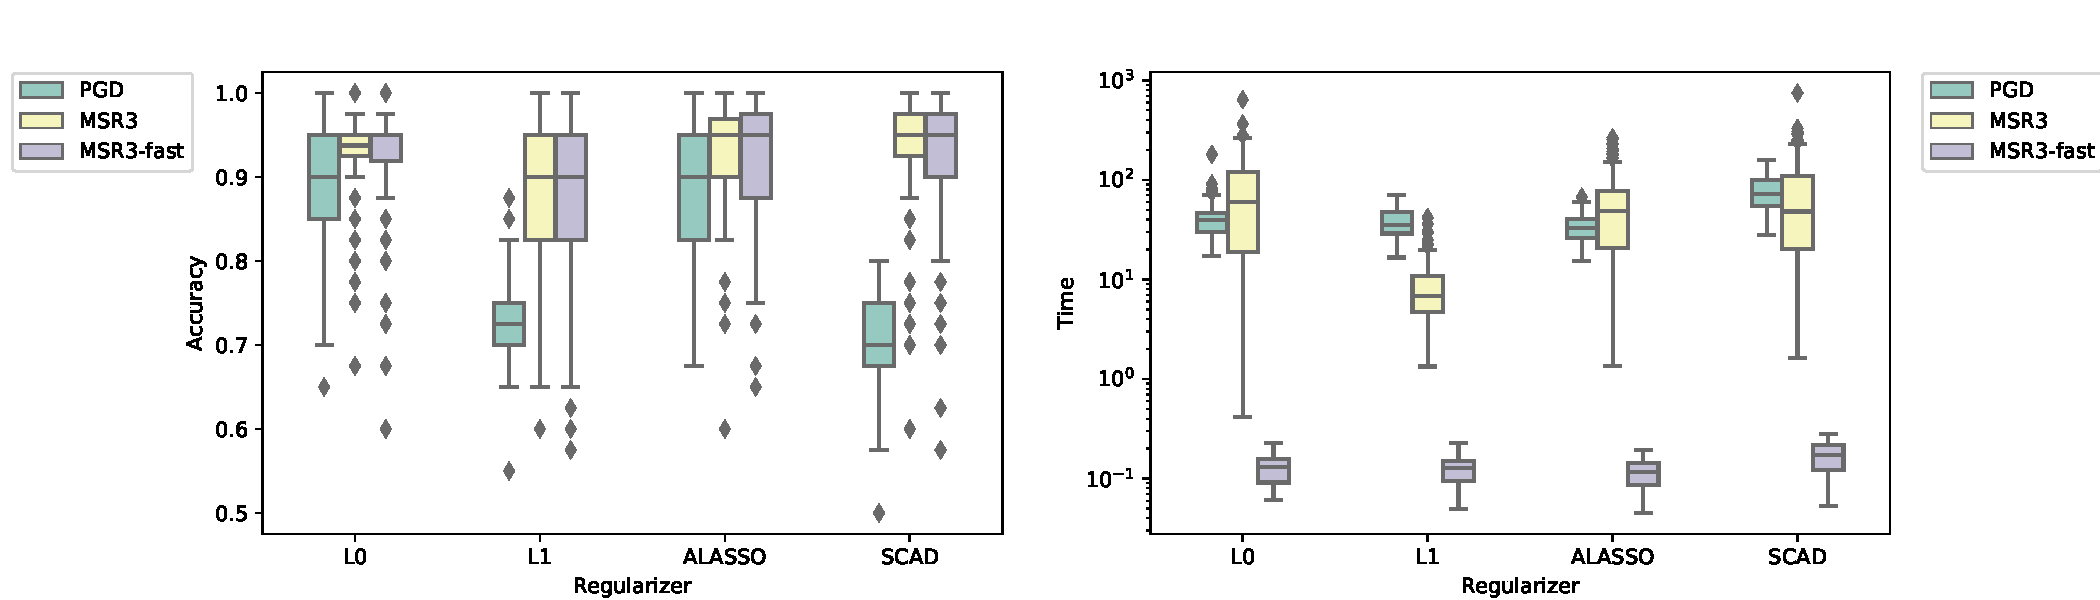
\includegraphics[width=1.0\textwidth]{figures/performance_picture_current}
	\caption{\label{fig:box_with_whiskers_for_synthetic_data}	Feature selection accuracy and execution time in seconds for PGD 
	(Algorithm \ref{alg:pgd_for_lme}), 
	MSR3 (Algorithm \ref{alg:pgd_for_value}), and MSR3-fast
	(Algorithm \ref{alg:pgd_for_value_function_fast}) with various regularizers. 
	MSR3-Fast has the same accuracy as 
	MSR3 and significantly decreases computation time.}
\end{figure}

In this section we 
{compare the numerical performance 
the feature selection accuracy and numerical efficiency of Algorithms 
\ref{alg:pgd_for_lme} and 
\ref{alg:pgd_for_value_function_fast} when using the 
LASSO, A-LASSO, SCAD, and L0 sparsity regularizers.
We begin by describing how the data is generated for our numerical simulations 
followed by a description of how the  
regularization parameter $\lambda$ and the coupling parameter $\eta$  were chosen.
Our experiments on real data are presented in Section \ref{sec:real}.}

%show the performance of the `regularization-agnostic' feature selection method, and also show that MSR3 improves performance across different regularization strategies. Specifically, we compare the feature selection accuracy and numerical efficiency of Algorithms  \ref{alg:pgd_for_lme} and 
%\ref{alg:pgd_for_value_function_fast} 
%with LASSO, A-LASSO, CAD, SCAD, and L0. 

%\paragraph{LASSO path} The LASSO path is a set of solutions $x$ parametrized by $\lambda$, where $\lambda$ is sweeping over its range from $\lambda = 0$ to $\lambda \to \infty$, until no parameters are included in the model. It's known that a classic LASSO tends to include false positives early along the path (\cite{Su2017}).


\paragraph{Experimental Setup.} The number of fixed effects $p$ and random effects $q$ are set at $20$ with $\beta = \gamma = [\frac{1}{2}, \frac{2}{2}, \frac{3}{2}, \dots, \frac{10}{2}, 0, 0, 0, \dots, 0]$, i.e. the first 10 covariates are increasingly important and the last 10 covariates are not. The data is generated as 
\[
\begin{aligned}
y_i &= X_i\beta + Z_iu_i + \varepsilon_i, \quad  \varepsilon_i \sim \NN(0, 0.3^2 I) \\
X_i &\sim \NN(0, I)^p, \quad Z_i = X_i \\ 
u_i& \sim \NN(0, \Diag{\gamma}),\\ 
\end{aligned}
\]
with 9 groups of sizes $[10, 15, 4, 8, 3, 5, 18, 9, 6]$. 
The data generation is repeated 100 times in order to estimate
the uncertainty bounds. The smallest non-zero components in the generated signals are just above the level of observation noise. 
%\red{We need to say something about "the smallest non-zero components are such that they are just above the noise from observation error"}

\vskip -.8in
\begin{wrapfigure}{r}{7.5cm}
		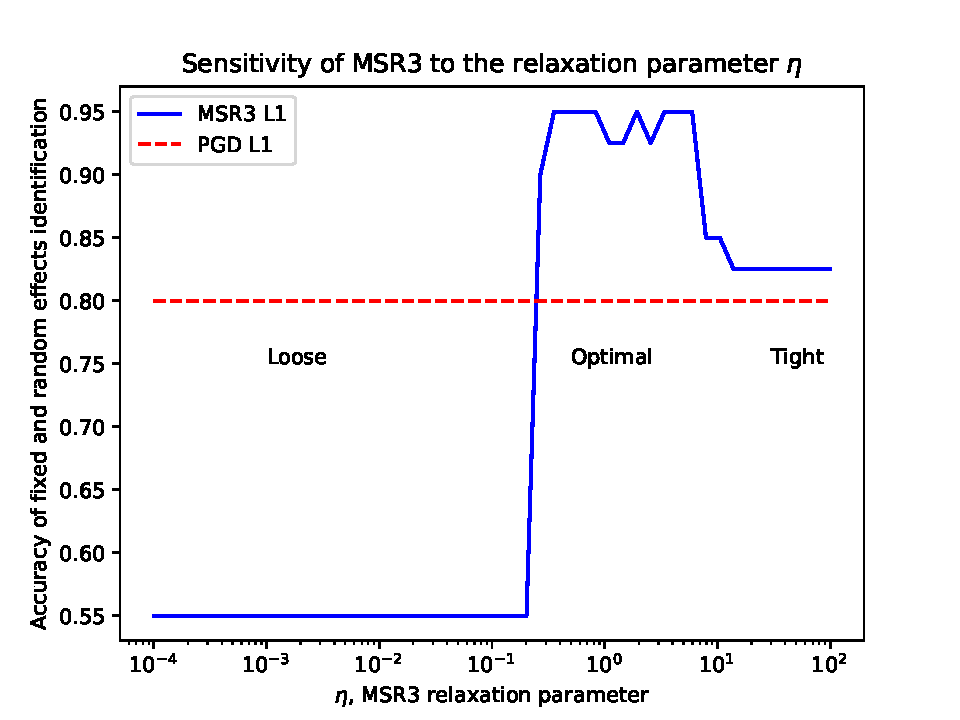
\includegraphics[width=7.5cm]{figures/eta_L1.pdf}
		\caption{Dependence of model performance on the relaxation $\eta$ for a sample problem.}\label{fig:eta}
	\end{wrapfigure} 
	

	
\paragraph{Parameter Selection.} The regularization parameter $\lambda$ 
multiplying $R$ and the 
coupling parameter $\eta$ restricting the difference between 
$(\beta,\gamma)$ and $(\tbeta,\tgam)$ are chosen to maximize a classic 
BIC criterion from \cite{Jones2011}. 
We begin by setting a log-uniform grid of 20 candidate values for the parameter $\eta \in [10^{-4}, 10^2]$, and then for each value of $\eta$
on this grid 
the BIC is optimized using a golden search in $\lambda \in [0, 10^5]$. The final values of $\eta$ and $\lambda$ are then chosen
to be those that maximize the BIC criterion.
	
	Figure \ref{fig:eta} shows the dependence of accuracy on the values of $\eta$ for the first data set generated in our test set. There are three distinct regions, corresponding to loose, moderate, and tight levels of coupling. When $\eta$ is small the coupling term does not have sufficient strength and the training does not progress far from the initial point (a fully dense vector \textbf{1} in this case). When the coupling is tight, the level-sets of the problem converge to those of the original problem, and thus the minimizer. For the values in between, the coupling significantly improves the model's accuracy. 
These results are consistent with experiments in the sparse linear regression setting~\cite{Zheng2019SR3}. 

\paragraph{Results.}
The experimental results are presented in the Table \ref{table:comparison_of_algorithms} and Figure~\ref{fig:box_with_whiskers_for_synthetic_data}. MSR3 improves the selection accuracy of most regularization techniques 
described in Table \ref{table:proxes}, showing a near-perfect performance, while converging two orders of magnitude faster in wall-clock time. 

\paragraph{Comparison to \texttt{glmmLasso} and \texttt{lmmLasso}.}
We used \cite[Table 3]{Buscemi2019Survey} as a reference 
for feature selection libraries. Of the 17 entries mentioned, the four libraries that successfully ran on our synthetic data described above were  packages \texttt{glmmLasso}\footnote{\href{https://rdrr.io/cran/glmmLasso/man/glmmLasso.html}{https://rdrr.io/cran/glmmLasso/man/glmmLasso.html}} (\cite{groll2014variable}), \texttt{lmmLasso}\footnote{\href{https://rdrr.io/cran/lmmlasso/}{https://rdrr.io/cran/lmmlasso/}}(\cite{schelldorfer2011estimation}), \texttt{fence}\footnote{\href{https://rdrr.io/cran/fence/}{https://rdrr.io/cran/fence/}} (\cite{jiang2008fence}) and \texttt{PCO} (\cite{lin2013pco}) libraries. \texttt{fence} caused a memory overflow on the experimental system during the performance evaluation on the datasets described above. We could not evaluate {\texttt{PCO} because
it did not support  datasets where the total number of random effects $mq$ exceeded the total number of observations $n$. We compare performance of MSR3 
(available through the open source \texttt{pysr3} library) 
to the performance of the \texttt{R} packages \texttt{glmmLasso}\footnote{\href{https://rdrr.io/cran/glmmLasso/man/glmmLasso.html}{https://rdrr.io/cran/glmmLasso/man/glmmLasso.html}} (\cite{groll2014variable}) and \texttt{lmmLasso}\footnote{\href{https://rdrr.io/cran/lmmlasso/}{https://rdrr.io/cran/lmmlasso/}} (\cite{schelldorfer2011estimation}) which are the functionally closest libraries available
} online. As of this writing, \texttt{glmmlasso} does not allow the user to specify $\Gamma$ as a diagonal matrix.  Since the diagonal specification simplifies the problem, this puts \texttt{glmmlasso} package at a disadvantage in our numerical comparison. We evaluate all algorithms' performance on the same set of problems as described above. We tuned the hyperparameters of \texttt{glmmLasso} and \texttt{lmmLasso} by minimizing the BIC scores provided by the libraries over $\lambda \in [0, 10^5]$. The results are presented in Table \ref{table:glmmlasso}. Overall, MSR3 executes, on average, 5 times faster in wall-clock time than \texttt{glmmLasso} and 60 times faster than \texttt{lmmLasso} and shows much higher accuracy of selecting correct fixed and random effects simultaneously. 
{The accuracy of \texttt{glmmLasso} is lower relative to the other libraries' scores likely due to its BIC selection criterion choosing dense models.} The package \texttt{lmmLasso} supports the diagonal specification of $\Gamma$, thus allowing a direct comparison with the scores from \texttt{pysr3}.  \texttt{lmmLasso} yields a competitive accuracy of selecting random effects but \texttt{lmmLasso} provides dense solutions for fixed effects $\beta$ for chosen values of $\lambda$. 

\begin{table}[ht]
\centering
\resizebox{\columnwidth}{!}{\begin{tabular}{lrrrr}
\toprule
Algorithm & Units (perc. / 100 runs) &         MSR3-Fast ($\ell_1$)&         glmmLasso &            lmmLasso \\
\midrule
Accuracy &\% (5\%-95\%)    &        {\bf 88 (72-98)} &        48 (42-55) &          66 (55-73) \\
FE Accuracy &\% (5\%-95\%) &      {\bf 86 (64-100)} &        52 (40-66) &          47 (45-55) \\
RE Accuracy &\% (5\%-95\%) &       {\bf 91 (74-100)} &        45 (45-45) &         84 (55-100) \\
F1          &\% (5\%-95\%)&        {\bf 89 (73-97)} &        63 (60-66) &           65 (0-77) \\
FE F1       &\% (5\%-95\%)&       {\bf 88 (69-100)} &        64 (57-70) &           57 (0-64) \\
RE F1       &\% (5\%-95\%)&       {\bf 90 (73-100)} &        62 (62-62) &          78 (0-100) \\
Time        &sec. (5\%-95\%)&  {\bf 0.19 (0.14-0.24)} &  1.37 (0.78-1.89) &  11.51 (5.35-23.66) \\
Iterations  & num. (5\%-95\%)&        {\bf 34 (28-45)} &        50 (33-77) &             - \\
\bottomrule
\end{tabular}
}

\caption{\label{table:glmmlasso} Comparison of performance of MSR3-Fast for $\ell_1$ regularizer vs \texttt{glmmLasso}. MSR3-Fast executes 5 times faster in wall time and has higher accuracy of selecting correct covariates. 
%Importantly, the accuracy of \texttt{glmmLasso} is likely skewed downwards due to BIC selection criterion choosing dense ultimate models and due to the missing option to constrain the matrix $\Gamma$ to be diagonal. \texttt{lmmLasso} supports the diagonal specification of $\Gamma$ which translates into a competitive quality of selecting random effects. However, while finding sparse fixed effects, \texttt{lmmLasso} provides dense solutions for fixed effects $\beta$.
}
\end{table}

\subsection{Scalability and Sensitivity Analysis}
\label{ch:msr3_sensitivity_analysis}
\subsubsection{Scalability}
We tested the scalability of the new approach (MSR3-fast) compared to proximal gradient descent and proximal gradient descent with line search. To do this, chose an initially small problem and we scaled the number of features in the data from 100 to 1000, while scaling the number of observations proportionally, and tested the time to completion 
of these three methods, averaged over 100 replicates. Namely, each problem had 8 groups of $10A$ observations each, $\beta$ and $\gamma$ had $20A$ features equally split between 0 and 1. To get the problems of different sizes we assigned $A$ to be 1, 2, 5, 10, 20, 50, and 100, and for each choice of A we generated 100 random problems. Since MSR3-fast has a relaxation parameter $\eta$, we evaluated MSR3-fast across different $\eta$ values to also test the effect of $\eta$ on timing. For each experiment, we also computed 
the accuracy of the feature selection, to make sure that there was no degradation in performance. The results are presented in Tables~\ref{table:scalability_time} and~\ref{table:scalability_accuracy}.  
In terms of timing, we indeed see a superlinear increase in computational complexity with respect to the number of features. Nonetheless, MSR3-fast is competitive with the alternatives across the experiments, and the results are far more accurate. 
Larger problems could likely significantly benefit from iterated solvers within the interior point framework. 

\begin{table}[ht]
	\centering
    \resizebox{\columnwidth}{!}{\begin{tabular}{l||lllllll|l|l}
\toprule
Algorithm & \multicolumn{7}{l}{MSR3-Fast} &       PGD & PGD-LineSearch \\
$\eta$ &     0.01  &    0.05  &    0.10  &    0.50  &    1.00  &     5.00  &     10.00 &    &         \\
\hline \hline 
\# Features &           &          &          &          &          &           &           &           &                \\
100                &     0m 7s &    0m 7s &    0m 7s &    0m 6s &    0m 7s &     0m 8s &    0m 10s &    2m 44s &         4m 44s \\
200                &    0m 36s &   0m 39s &   0m 36s &   0m 39s &   0m 39s &    0m 49s &     1m 8s &    7m 43s &        11m 28s \\
400                &     5m 2s &   4m 51s &   4m 34s &   4m 26s &   5m 16s &    7m 33s &   10m 38s &   47m 46s &        12m 36s \\
1000               &   59m 10s &  57m 12s &  60m 30s &  69m 57s &  68m 55s &  111m 31s &  139m 47s &  469m 16s &         55m 8s \\
\bottomrule
\end{tabular}
}
    \caption{Execution time for feature selection problems of varying sizes. Each cell shows total time, including grid-search with respect to the sparsity parameter $\lambda$. Each cell shows averaged value over 100 randomly-generated problems.}
    \label{table:scalability_time}

\end{table}

\begin{table}[ht]
	\centering
    %\resizebox{\columnwidth}{!}{}
    \begin{tabular}{l||rrrrrrr|r|r}
\toprule
Algorithm & \multicolumn{7}{l}{MSR3-Fast} &   PGD & PGD-LineSearch \\
$\eta$ &     0.01  & 0.05  & 0.10  & 0.50  & 1.00  & 5.00  & 10.00 &   &           \\
\hline \hline
\# Features &           &       &       &       &       &       &       &       &                \\

100                &      0.94 &  0.94 &  0.95 &  0.94 &  0.91 &  0.86 &  0.84 &  0.77 &           0.77 \\
200                &      0.99 &  0.99 &  0.99 &  0.98 &  0.98 &  0.97 &  0.95 &  0.78 &           0.82 \\
400                &      0.99 &  0.99 &  0.99 &  0.99 &  0.99 &  1.00 &  1.00 &  0.80 &           0.84 \\
1000               &      0.99 &  0.98 &  0.98 &  0.98 &  0.98 &  1.00 &  1.00 &  0.83 &           0.87 \\
\bottomrule
\end{tabular}

    \caption{Accuracy of feature selection problems of varying sizes. Each cell shows averaged value over 100 randomly-generated problems.}
    \label{table:scalability_accuracy}
\end{table}


\subsubsection{Closeness to the Central Path for IP}
The $\tau$ parameter of MSR3-fast controls how close the interior point method gets to the central path before taking a prox-gradient step. This is a heuristic parameter in the algorithm, and to understand its impact we tested 
the sensitivity of the execution time and accuracy for a problem with 200 features for four selections of relaxation parameter $\eta$. The problems were identical to those from the second row of Table~\ref{table:scalability_time}. The results are reported in Tables~\ref{table:central_path_time} and~\ref{table:central_path_accuracy}. 
Neither time nor accuracy were affected by $\tau$ across the levels of $\eta$. 

\begin{table}[ht]
	\centering
    \begin{tabular}{l||llll}
\toprule
Algorithm & \multicolumn{4}{l}{MSR3-Fast} \\
$\eta$ &     0.01  &   0.10  &   1.00  &   10.00 \\
\hline \hline
$\tau$ &           &         &         &         \\
0.1 &    0m 41s &  0m 40s &  0m 41s &  1m 12s \\
0.3 &    0m 35s &  0m 36s &  0m 38s &   1m 1s \\
0.5 &    0m 34s &  0m 35s &  0m 36s &  0m 57s \\
0.7 &    0m 33s &  0m 33s &  0m 35s &  0m 59s \\
0.9 &    0m 33s &  0m 33s &  0m 35s &  0m 52s \\
\bottomrule
\end{tabular}

    \caption{Execution time of MSR3-fast for different values of $\tau$ - a parameter that controls how close the IP needs to be to the central path before doing a projection step. Each cell shows total time, including grid-search with respect to the sparsity parameter $\lambda$. Each cell shows averaged value over 100 randomly-generated problems.}
    \label{table:central_path_time}
\end{table}

\begin{table}[ht]
	\centering
    %\resizebox{\columnwidth}{!}{}
    \begin{tabular}{l||rrrr}
\toprule
Algorithm & \multicolumn{4}{l}{MSR3-Fast} \\
$\eta$ &     0.01  & 0.10  & 1.00  & 10.00 \\
\hline \hline
$\tau$ &           &       &       &       \\
0.1 &      0.99 &  0.99 &  0.99 &  0.95 \\
0.3 &      0.99 &  0.99 &  0.98 &  0.95 \\
0.5 &      0.99 &  0.99 &  0.98 &  0.95 \\
0.7 &      0.99 &  0.99 &  0.98 &  0.95 \\
0.9 &      0.99 &  0.99 &  0.98 &  0.95 \\
\bottomrule
\end{tabular}

    \caption{Accuracy of MSR3-fast for different values of $\tau$ - a parameter that controls how close the IP needs to be to the central path before doing a projection step. Each cell shows averaged value over 100 randomly-generated problems.}
    \label{table:central_path_accuracy}
\end{table}




\subsection{Application to Real Data: Anxiety and Depression as a Result of Bullying Victimization}
\label{sec:real}

\begin{figure}
    \centering
	\caption{\label{fig:bullying_data_random_feature_selection}Validation of Random Feature Selection for Bullying Data from GBD 2020. 
	Left panel shows coefficient paths across numbers of nonzero covariates allowed in the model using the $\ell_0$ regularizer. 
	Right panel evaluates each choice against expert knowledge. 
	The algorithm picks seven historically significant covariates and two historically insignificant, for the model selected using the BIC criteria. 
	See the Appendix \ref{appendix:bullying_covariates} for covariates description and assessment of significance.}
	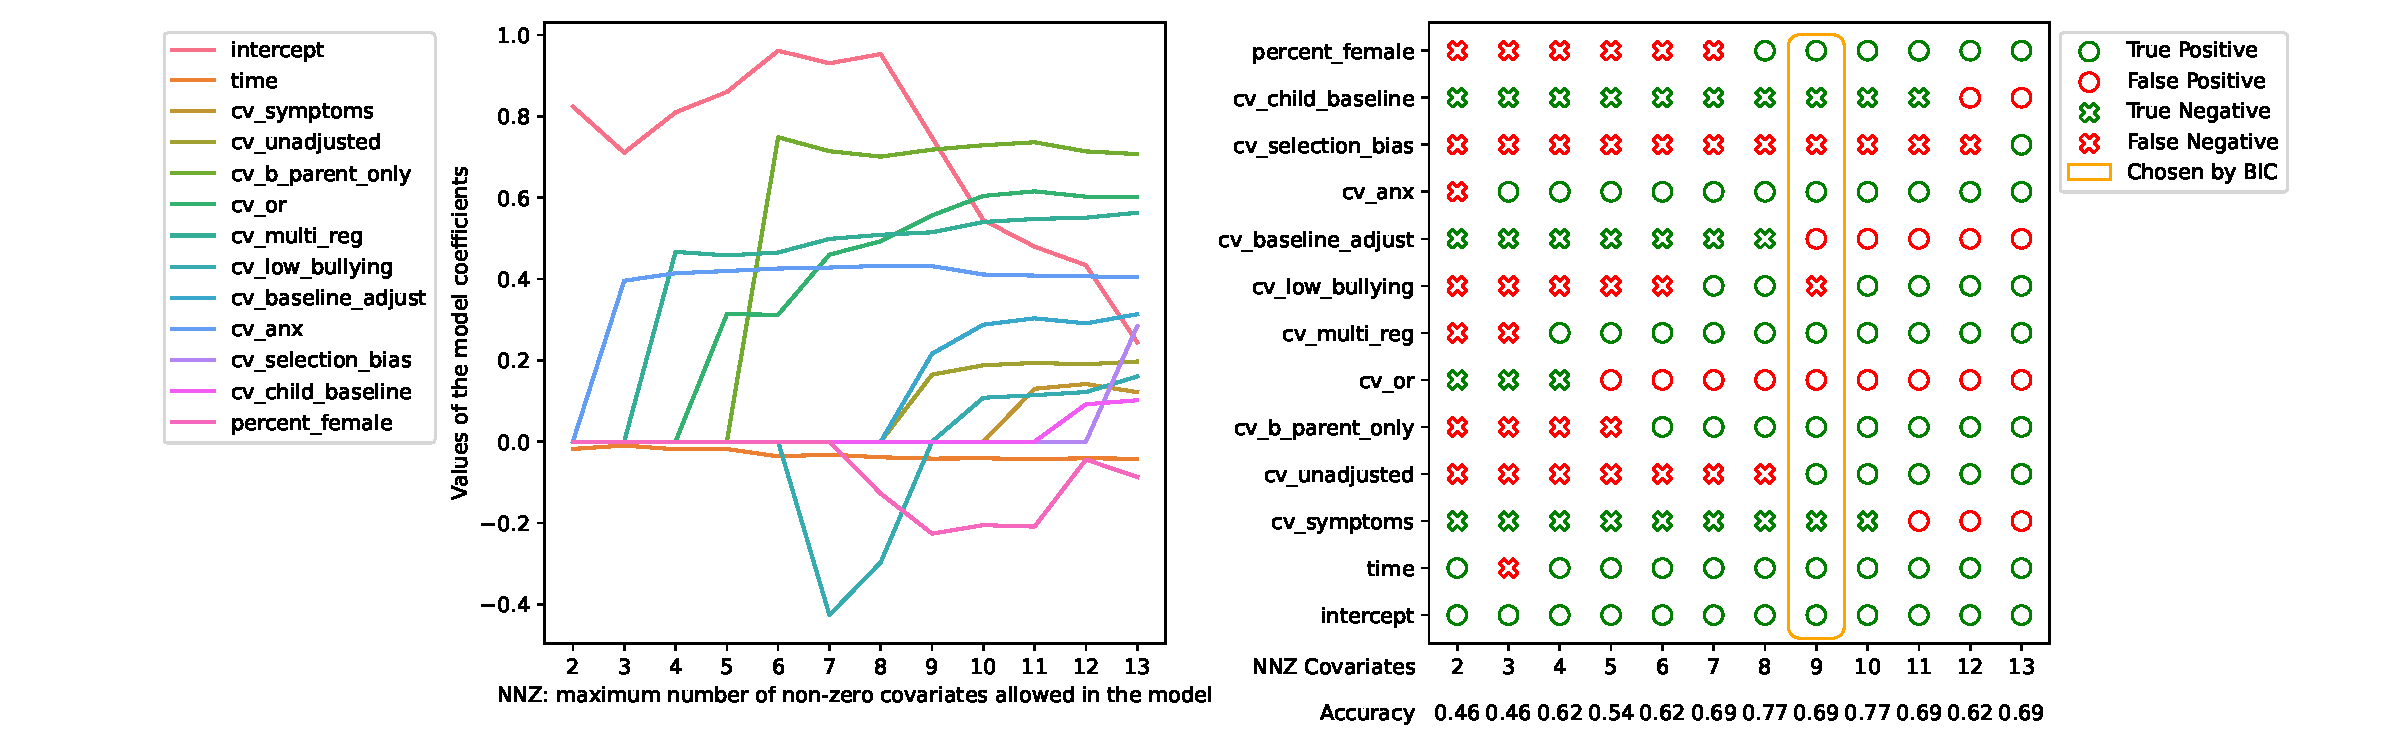
\includegraphics[width=1\textwidth]{figures/bullying_data_assessment_selection}
\end{figure}

In this section we validate the MSR3-empowered $\ell_0$-regularized mixed-effect model ($R(x) = \delta_{\|x\|_0 \leq k}$ from Table \ref{table:proxes}) by using it to identify the most important covariates in real data on relative risk of anxiety and depressive disorders depending on the exposure to bullying in young age\footnote{Institute for Health Metrics and Evaluation (IHME). Bullying Victimization Relative Risk Bundle GBD 2020. Seattle, United States of America (USA), 2021.}. This research has been a part of Global Burden of Diseases study for the last several years. The end goal  is to estimate the burden 
{through disability adjusted life years} (DALYs)~\citep{murray1997understanding}
of major depressive disorder (MDD) and anxiety disorders that are caused by bullying. For this risk factor, the exposure is primarily concentrated in childhood and adolescents, but the risk for MDD and anxiety disorders is anticipated to continue well into adulthood. This elevated risk is, however, expected to decrease with time as other risk factors come into play in adulthood (unemployment, relationship issues, etc.). To accommodate this, the research team uses the models which estimate the relative risk (RR) of MDD and anxiety disorders among persons exposed to bullying depending on how many years it has been since the first exposure. Studies informing the model were sourced from a systematic review and consist of longitudinal cohort studies. They measure exposure to bullying at baseline, and then follow up years later and assess them for MDD or anxiety disorders. The detailed description of the covariates can be found in Appendix \ref{appendix:bullying_covariates}.

The feature selection process is illustrated on Figure~\ref{fig:bullying_data_random_feature_selection}. 
%Since there is no prior on $k$ -- the number of features to keep in the model -- 
Here, the BIC criterion from \cite{Jones2011} was used to select $k$, which suggests $k=4$ or $5$.  
 For the $k=4$ case, the selected covariates (\texttt{intercept}, \texttt{time}, \texttt{cv\_threshold\_bullying}, \texttt{cv\_b\_parent\_only}) 
are known as important and were used in the analysis in previous years of GBD. For the $k=5$ case, 
%five covariates (in addition to \texttt{intercept} and \texttt{time}) were selected by \ouralgo: \texttt{cv\_unadjusted}, \texttt{cv\_threshold\_bullying}, \texttt{cv\_b\_parent\_only}, \texttt{cv\_anx}, and \texttt{percent\_female}. 
%in addition to the covariates already known to be important, 
the algorithm also selects  \texttt{cv\_child\_baseline} and \texttt{cv\_or}, which were not used before. The  \texttt{cv\_child\_baseline} covariate describes whether the midpoint in the sample is above or below 13. 
The  \texttt{cv\_or} variable describes whether the estimate is a relative risk or odds ratio. The selection of these variables suggests a closer look at the data reporting mechanisms across studies. 
For example, there is an active literature on converting estimates between relative risks and odds ratios~\cite{grant2014converting,wang2013converting}.

\subsection{Application to Real Data: COVID-19 Transmission Factor}
\label{ch:covid}
\begin{figure}
	\begin{subfigure}[b]{\textwidth}
		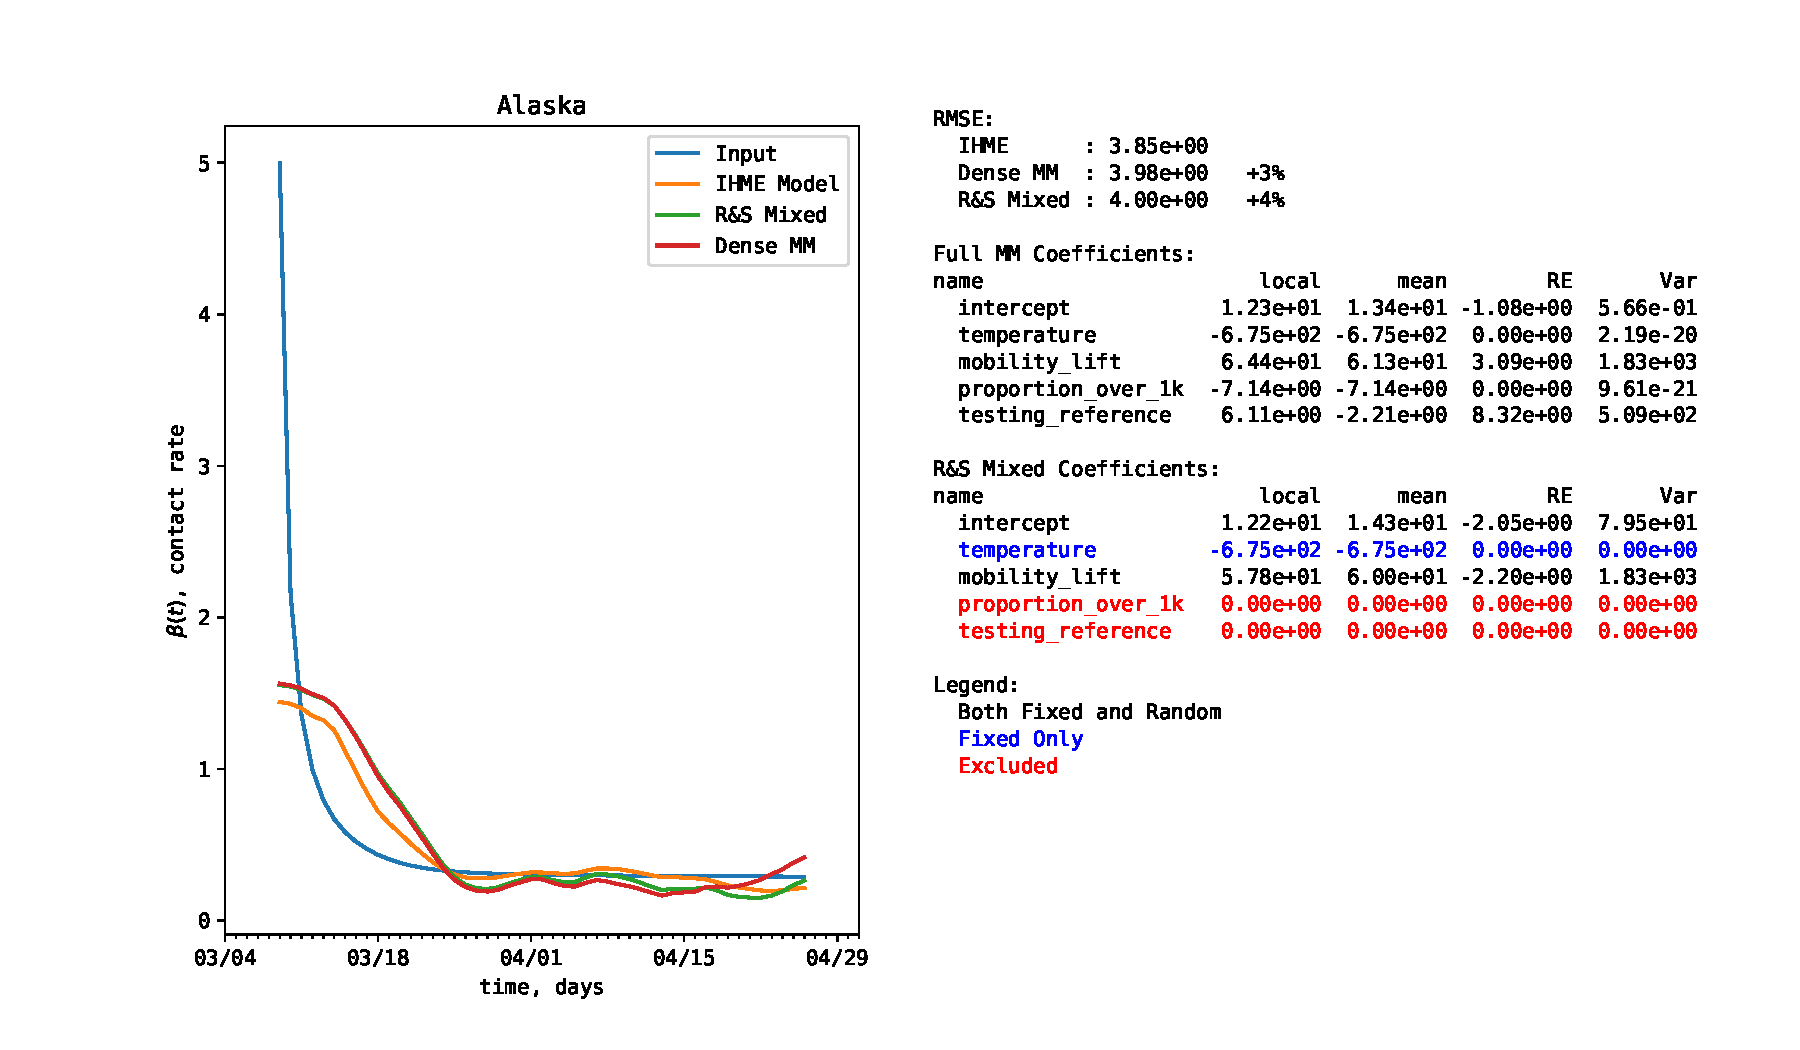
\includegraphics[width=\textwidth]{figures/fit_Alaska}
	\end{subfigure}
	\begin{subfigure}[b]{\textwidth}
		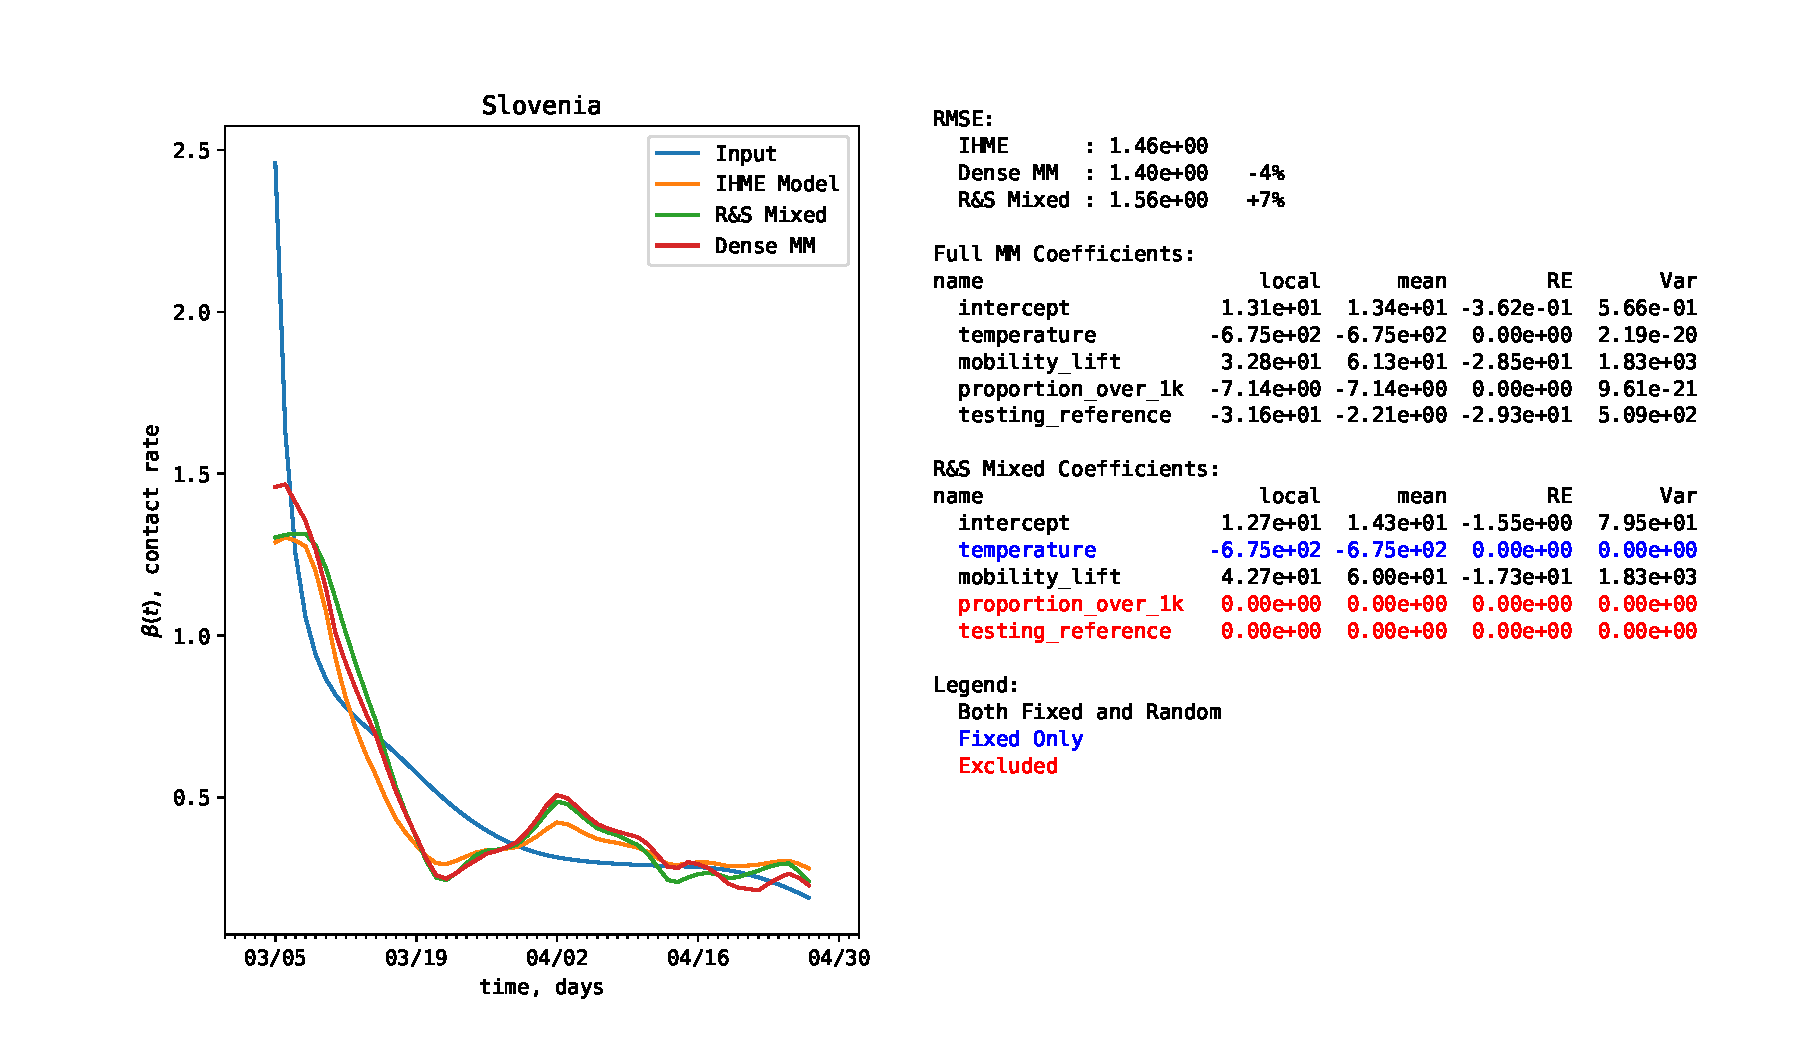
\includegraphics[width=\textwidth]{figures/fit_Slovenia}	
	\end{subfigure}
	\caption{\label{fig:covid_feature_selection_1} Comparison of fits of two different models (fully dense linear mixed model(MM) and MSR3-$\ell_0$ (R\&S) to the original IHME Projections for Alaska and Slovenia. The quality (RMSE) achieved by a sparse fit is within 10\% from a quality of both dense models which is evidences that the model picked up informative features.}
\end{figure}

\begin{figure}
	\begin{subfigure}[b]{\textwidth}
		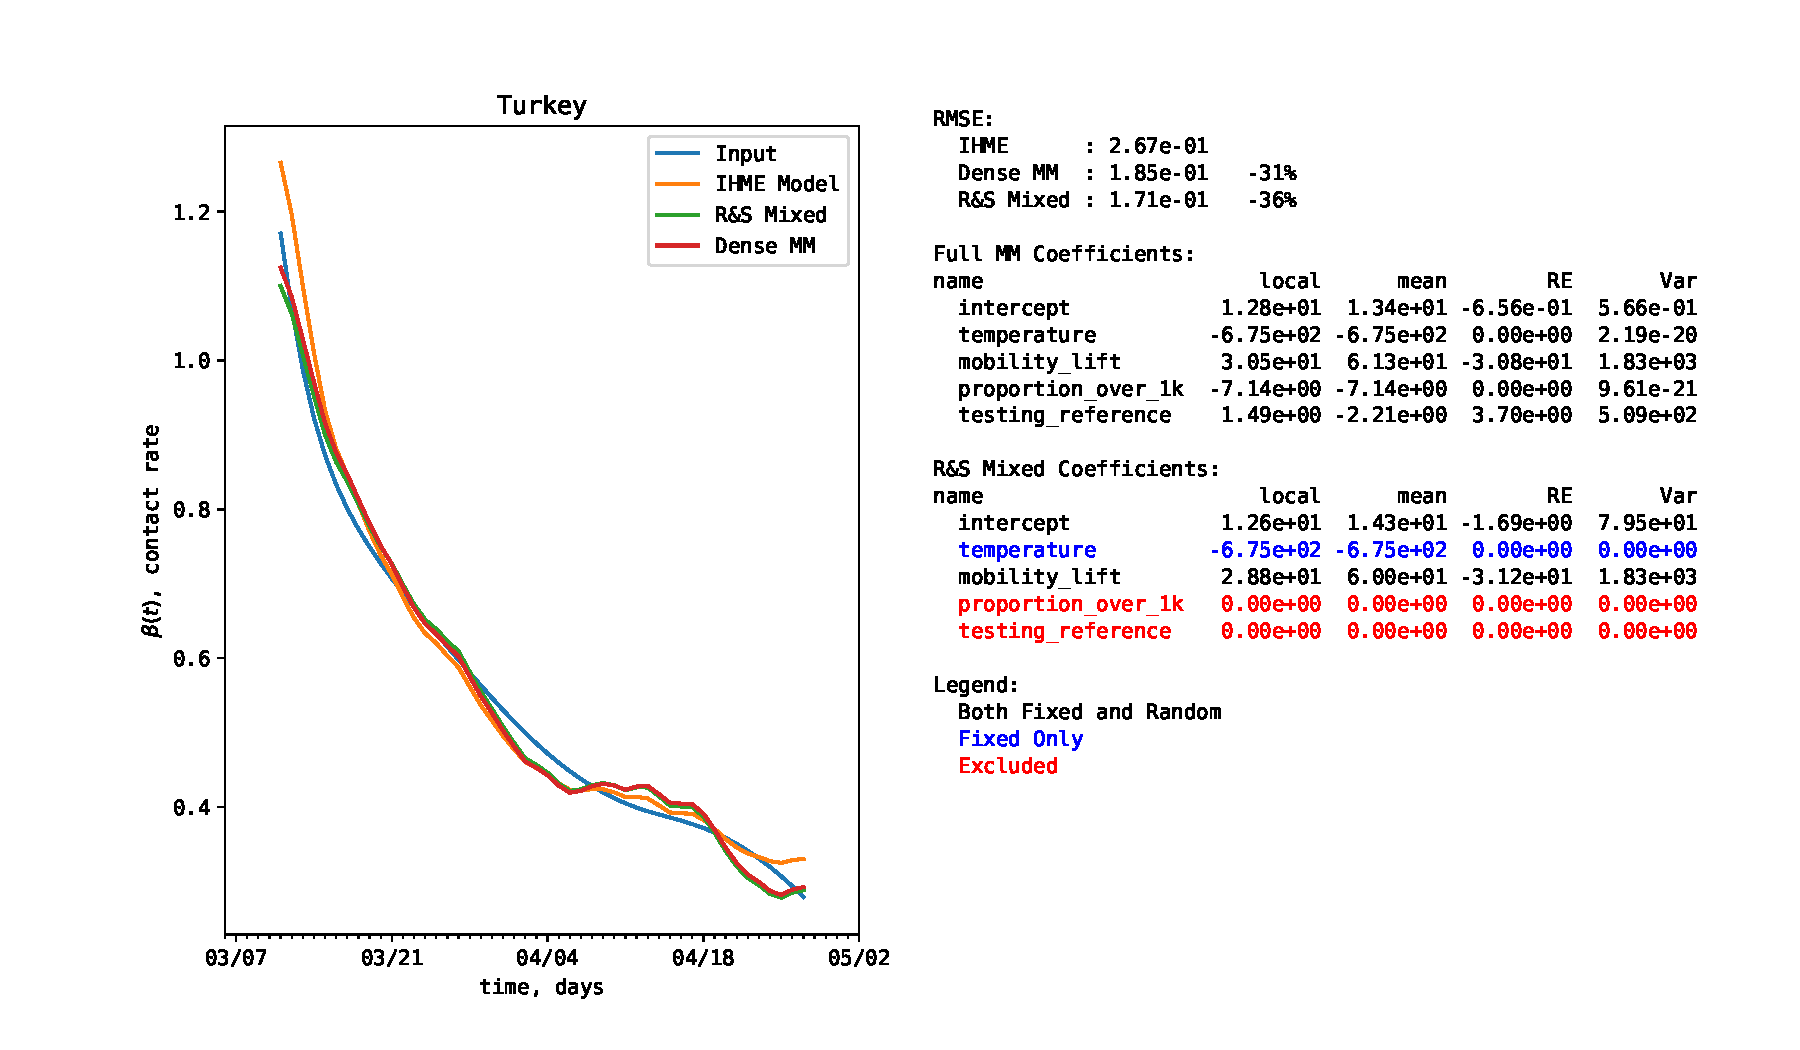
\includegraphics[width=\textwidth]{figures/fit_Turkey}
	\end{subfigure}
	\begin{subfigure}[b]{\textwidth}
		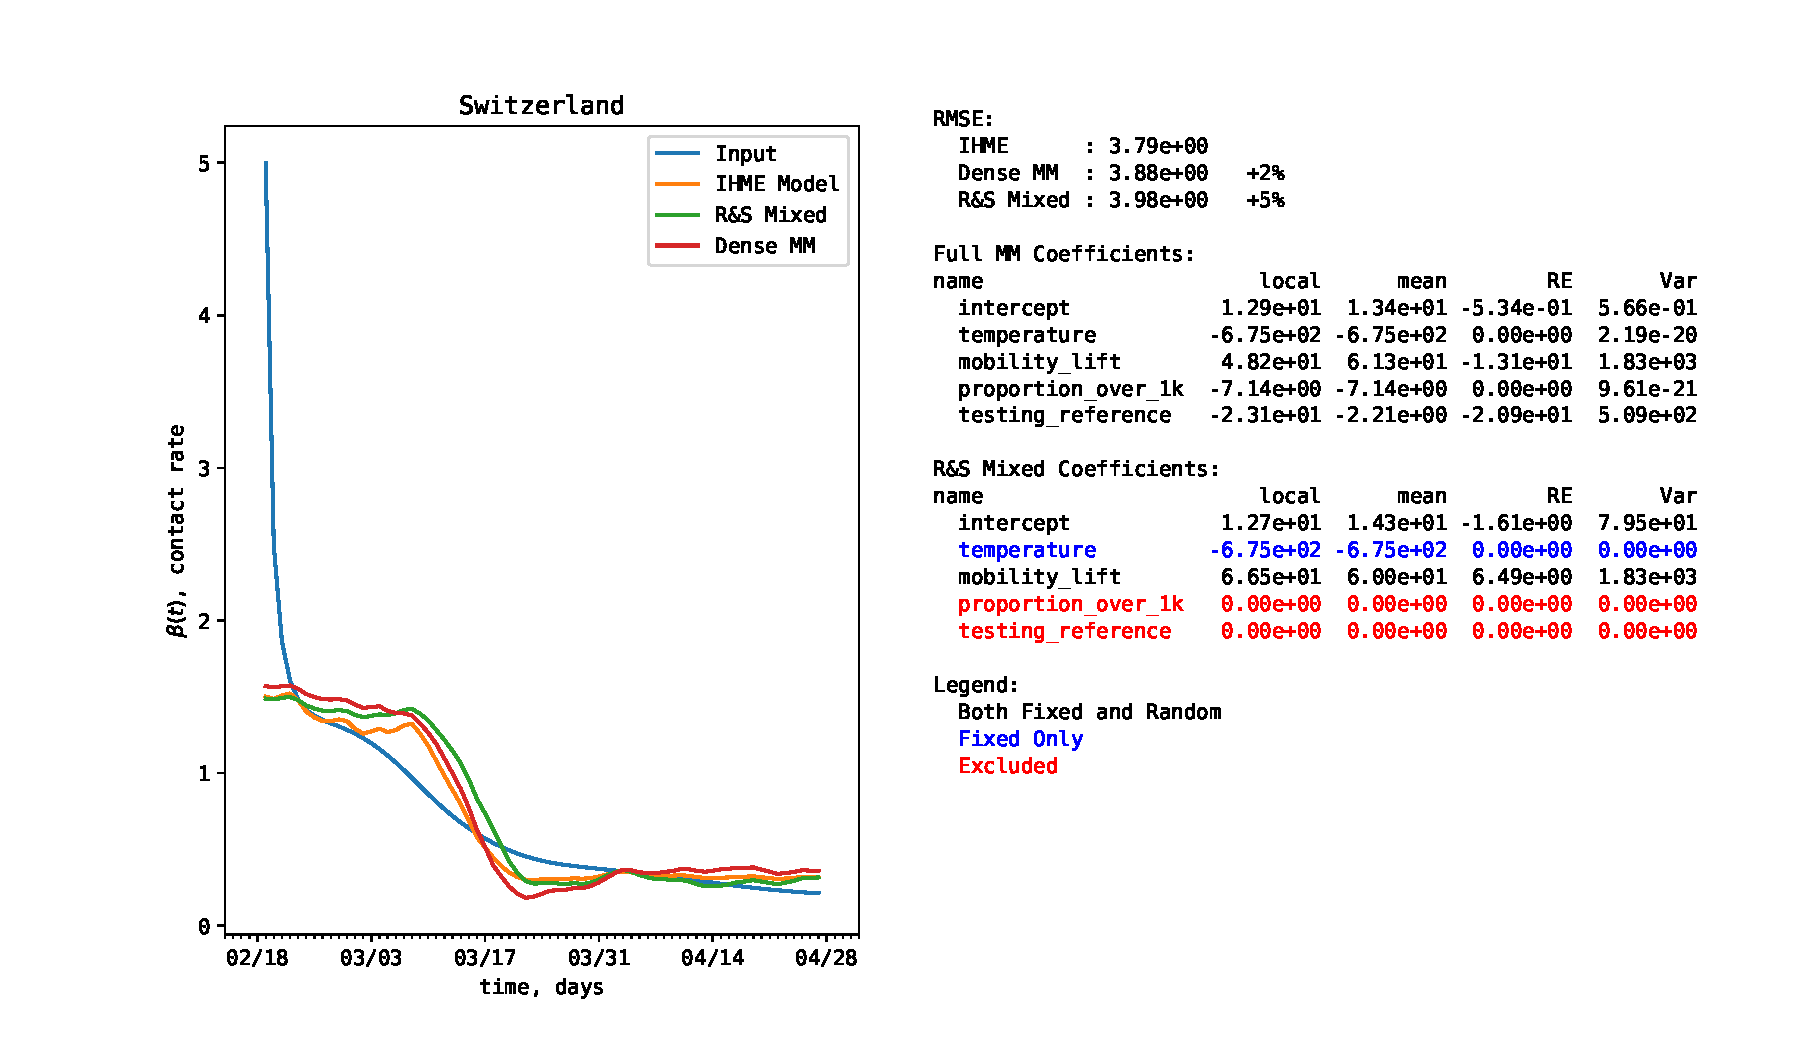
\includegraphics[width=\textwidth]{figures/fit_Switzerland}	
	\end{subfigure}
	\caption{\label{fig:covid_feature_selection_2} Comparison of fits of two different models (fully dense linear mixed model (MM) and MSR3-$\ell_0$) (R\&S) to the original IHME Projections for Turkey and Switzerland. The quality (RMSE) achieved by a sparse fit is within 10\% from a quality of both dense models which is evidences that the model picked up informative features.}
\end{figure}

In this section we apply our method to a COVID-19 Contact Rate Forecasting problem. The global pandemic created an unprecedented need for robust and accurate disease transmission forecasting. Since the beginning of the pandemic Institute for Health Metrics and Evaluation has been providing guidance to local authorities across the world with their pioneering \href{https://covid19.healthdata.org/global?view=total-deaths&tab=trend}{COVID-19 Projections tool} \cite{IHME2020Projections}. The key methodology which was essential for success in their forecasting of the disease's dynamics was transforming the death data into the contact rate time series data, and then relating this contact rate to available covariates such as temperature, social mobility, population, and others \cite{IHME2020covidnature}. All these covariates were collected in real time using limited human resources, and identifying the most important covariates was crucial for distributing these resources effectively. In the example below we show how \ouralgo can be used for making covariate selection on IHME data. 


The dataset consists of $m=60$ groups (countries or states), the detailed description of groups sizes ($n_i$) and time spans is provided in the Appendix~\ref{ch:covid}. The target variable $Y_i$ was the contact rate -- the coefficient $\beta(t)$ from an SEIR model (not to be confused with $\beta$ -- vector of fixed effects). The covariates -- columns of $X_i$ and $Z_i$ -- were: \texttt{intercept} --a column of ones,  \texttt{temperature} -- average air temperature in degrees Fahrenheit, \texttt{mobility\_lift} -- social mobility, \texttt{proportion\_over\_1k} -- population size threshold, and \texttt{testing\_reference} -- testing. The observation error's variance $\sigma_i$ was set to be 0.1.

Feature selection results for four particular locations (Alaska, Slovenia, Turkey, and Switherland) are presented on Figures \ref{fig:covid_feature_selection_1} and \ref{fig:covid_feature_selection_2}, with coefficients for the rest of the locations attached in supplementary materials. \ouralgo was charged with a task to produce a fit using only three covariates, one of which had to be mean-only (no random effects). On the left we see the original data (\texttt{Data}, in {\color{blue} blue}), and predictions of three models: IHME Projections (\texttt{IHME}, in {\color{orange} orange}), a linear mixed model fit with no selection (\texttt{Dense MM}, in {\color{red} red}), and a sparse fit of \ouralgo (\ouralgo in {\color{green} green}). The \ouralgo model has chosen to use \texttt{intercept}, \texttt{mobility\_lift}, and \texttt{temperature} covariates, with the later only as a fixed covariate; \texttt{testing\_reference} and \texttt{proportion\_over\_1k} were left out. On the plots to the left we see that the exclusion of two covariates did not significantly affect the quality of predictions. The residual errors (RMSE) to the right support this statement: the difference in RSME is within 10\% of RSME of a "dense" model which uses all the covariates, as well as from IHME's original model which fit all the locations via sequence of independent regressions. This choice also seems reasonable given the timespan: the proliferation of testing during the spring was not yet significant, so it did not inform predictions in a major way. The exclusion of \texttt{proportion\_over\_1k} could have been due to the scale of grouping: locations were grouped on the level of states and countries, not on the level of individual counties where the influence of population-based covariates could have been more significant. 




\section{Theoretical Analysis}
%gives the problem structure used in the design of our
%numerical solution method. 
%Specifically, we design a 
%(PGD) %prox gradient 
%method 
%for solving this problem (see Section \ref{sec:pgd}). For this we must show that the function $u_\emu$
%is continuously differentiable with Lipschitz continuous gradient. 

%\section{Prox Gradient Descent}
\subsection{Proximal Gradient Descent for \texorpdfstring{$\uemu\tbg + R\tbg+\del_{\Rqp}(\tgam)$}{}} 
\label{sec:pgd}

We follow the analysis of the PGD algorithm given in \cite[Chapter 10]{AB17}
as it applies to the objective
%The application of the (PGD) %proximal gradient descent 
%algorithm to 
\begin{equation}\label{eq:varphi}
\Phi_\emu\tbg:=\uemu\tbg +\tR\tbg,\ \ \text{where}\ 
\tR\tbg:=R\tbg+\del_{\Rqp}(\tgam).
\end{equation}
%
%We now state the (PGD) %prox gradient descent 
%algorithm for finding a minimum for \eqref{eq:relax3}. 
Since $u_\emu$ is nonconvex, one typically 
applies a line search method to select stepsize. 
However, this is often not required in practice. 
For this reason we state the algorithm with and without a line search.
\medskip

%, as outlined in Algorithms \ref{alg:pgd_for_lme} and \ref{alg:MSR3}. 
%Set $\hR\tbg=R\tbg+\del_{\R^q_+}(\tgam)$ and 
%$\phi\tbg:=u_\emu\tbg+\hR\tbg$.
%See also Appendix 
%\smallskip

%\noindent
%{\bf Algorithm 1:} Proximal Gradient Descent with fixed stepsize (PGD)


%\noindent
%{\bf Algorithm 2:} Proximal Gradient Descent with Backtracking (PGD-B)

\begin{algorithm}[ht]
\SetAlgoLined
{\bf Initialize:} 
$\theta\in(0,1),\ \tau\in(0,1)$,
$\eta>0,\ \mu>0$, $\eps_{\mbox{\tiny Tol}}\ge 0$
$k=0$, $t_0>0$, $\bw^{0}=(\tbeta^0,\tgam^0)\in \Rp\times\R^q_+$
with $\inf\Phi_\emu <\Phi_\emu(\bw^0)$, 
$\gammax>\tgam^0$, 
$w^0=\prox_{t_0\tR}(\bw^{0}-t_0\nabla u_\emu(\bw^0))$.
%$, \ \eta_{Tol}\ge\eta_0>0,\ \mu_0\ge \mu_{Tol}>0$.
\\
\While{{\small $\norm{w^k-\bw^k}>\eps_{\mbox{\tiny Tol}}$
and $\gam^k\le\gammax$}}{\small\smallskip
\begin{enumerate}
\item[(i)] $t_{k+1}=\max\lset{t}{
\begin{aligned}&s\in\bW,\, t=t_0\theta^s,\ 
w=\prox_{t\tR}(w^k-t\nabla u_\emu(w^k))\\ &
\phi(w)
\le \phi(w^k)-\tau t\norm{w^k-w}^2
\end{aligned}}$.
\item[(ii)] $\bw^{k+1}=w^{k}$
\item[]$w^{k+1}=\prox_{t_{k+1}\tR}(w^k-t_{k+1}\nabla u_\emu(w^k))$
\item[]$k=k+1$
\end{enumerate}
}
\smallskip
\caption{\label{alg:pgd with bt}Proximal Gradient Descent 
fo $\Phi_\emu$ with Backtracking}
\end{algorithm}
\medskip


In Algorithm \ref{alg:MSR3}, 
the parameter $L$ is assumed to be a global Lipschitz
constant for $\nabla \uemu$. In Section \ref{sec:convergence pgd}, we show that the existence of $L$ is not needed.
In both algorithms we introduce the requirement that $\gam^k\le\gammax$.
While it is possible to include an explicit constraint of this form in the 
optimal variable selection problem \eqref{eq:lme_loss_original_in_x}, 
we do not do so since we assume that $\gammax$ is chosen 
so large that, from a practical perspective, 
the violation of this constraint indicates that the model is 
poorly posed and the algorithm needs to be terminated.
We base our analysis of the convergence properties of
Algorithms 1 and 2 on \cite[Theorem 10.15]{AB17} which makes use
of the following three basic assumptions:
\smallskip

\noindent
{\bf Basic Assumptions for the PGD Algorithm}
\begin{enumerate}
\item[(A)] $\map{\tR}{\Rp\times\Rq}{\eR}$ is a closed proper convex function.
\item[(B)] $\map{\uemu}{\Rp\times\Rq}{\eR}$ is closed and proper, 
$\dom{\uemu}$ is
convex, $\dom{\tR}\subset\intr{\dom{\uemu}}$, and
$\uemu$ is $L_\emu$-smooth over $\intr{\dom{\uemu}}$.
\item[(C)] Problem \eqref{eq:relax3} has an optimal solution with optimal 
value $\Phi_{\mbox{\tiny OPT}}$.
\end{enumerate}

\noindent
We assume that (A) holds. This is not an overly
restrictive assumption since it is satisfied by most of the standard
variable selection regularizers.
We show that (C) holds when $R$ satisfies
an additional coercivity hypothesis (Theorem \ref{thm:relaxed existence}). 
On the other hand, establishing that (B) holds
in a concrete setting such as ours
can be quite difficult. 
In particular, just as with $\LL$, $\uemu$ may fail to be globally Lipschitz.
Validating Assumption (B) as well as developing a technique for circumventing
the need for a global Lipschitz constant for $\nabla\uemu$ 
consumes the majority of the theoretical development. 
%Assumption (B) is particularly difficult since $\uemu$ is an optimal value function.
%We establish $B$ established in several steps.
%However, we show that the global Lipschitz continuity of $\nabla \uemu$
%is not required in practice for the theory developed in 
%\cite{AB17} to apply. 
%We begin by establishing the smoothness of $\uemu$.

%\begin{figure}[ht]
%    \centering
%    \includegraphics[width=\textwidth]{Images/intuition_current.pdf}
%    \caption{Proximal Gradient Descent (PGD) takes an order of magnitude fewer iterations to converge when optimizing a value function instead of the original likelihood, because SR3-relaxation improves the conditioning of the problem, which results in a more spherical level-sets. This effect persists for both quadratic convex (first row) and non-convex components (second row) of the likelihood. The effect is stronger for  minima near the boundary of the constraint region 
%    (bottom-left panel).}
%    \label{fig:geometric_intuition_sr3}
%\end{figure}


\subsection{The Smoothness of \texorpdfstring{$u_\emu$}{}}\label{sec:smoothness}
We investigate the relationship between the problems \eqref{eq:lme_loss_original_in_x}
and \eqref{eq:relax2}, the existence of solutions to 
 \eqref{eq:relax2}, and the properties of the function $\uemu$ and its derivative.
%We begin with an examination of the function $\LL$
%and 
%The first step is to understand the role of the parameter $\blam$.

\subsubsection{Underlying convexity}

\begin{lemma}[$\LL+\phimu$ is Weakly Convex]\label{lem:LL weak cvx}
Let $\LL$ be as given in \eqref{eq:lme_diagonal_setup}. Then
\begin{equation}\label{eq:hess LL}
\nabla^2\LL{(\beta,\gam)}=\sum_{i=1}^m
S_i^T\begin{bmatrix}X_i^T\\ -Z_i^T\end{bmatrix}
\Omega_i(\gam)^{-1}
\begin{bmatrix}X_i& -Z_i\end{bmatrix}S_i
-\begin{bmatrix}
0&0\\ 0& \half(Z_i^T\Omega_i(\gam)^{-1}Z_i)^{\circ2}
\end{bmatrix},
\end{equation}
for all
$(\beta,\gam)\in\R^p\times\R^q_+$, where 
\[
S_i:=\begin{bmatrix}
I_q&0\\ 0&\Diag{Z_i^T\Omega_i^{-1}(X_i\beta-Y_i)}
\end{bmatrix}
\]
and, for any $A\in\R^{t\times t}$, $A^{\circ 2}:=A\circ A$. In particular, this implies
that the matrix
\begin{equation}\label{eq:psd for LL}
\begin{bmatrix}
\nabla_{\beta\beta}\LL(\beta,\gam)&\nabla_{\gam\beta}\LL(\beta,\gam)\\
\nabla_{\beta\gam}\LL(\beta,\gam)&\nabla_{\gam\gam}\LL(\beta,\gam)
+\blam I\end{bmatrix}
\end{equation}
is positive semidefinite
for $\bar\eta= \nu m$, where
\[
\nu:=max\lset{(1/2) \mu_\mmin(\Lam_i)^{-2}\sig^4_\mmax(Z_i)}{i=1,\dots,m},
\]
$\mu_\mmin(\Lam_i)$ is the smallest eigenvalue of $\Lam_i$, and
 $\sig_\mmax(Z_i)$ is the largest singular value of $Z_i,\, i=1,\dots,m$.
Consequently, for any $\tbg\in\dom{\tR}$ and $\mu\ge 0$, the mapping 
\(
\bg\mapsto \LL_{\emu}(\bg, \tbg)
%\hLL(\bg,\tgam) %:=\LL(\beta,\gam)+\frac{\blam}{2}\norm{\gam-\hgam}^2
%\sum_{i=1}^m\frac{\nu_i}{2}\norm{\gam-\hat\gam}^2,
\)
is convex for all $\eta\ge\bar\eta:=\nu m$.
In particular, this implies that $\LL+\phimu$ is weakly convex for any $\mu\ge 0$, 
and the mapping
\(
%\begin{aligned}
\bg\mapsto\LL_{\emu}(\bg,\tbg)
%&=
%\LL\bg+\phimu(\gam)+
%\keta(\beta-\tbeta,\beta-\tbeta)
%\\ &=
%\hLL(\bg,\tgam)+    \frac{\eta}{2}\norm{\bg-\tbg}^2 
%\end{aligned}
\)
is strongly convex for $\eta> \bar\eta$ with modulus of strong convexity $(\eta-\bar\eta)$
regardless of the choice of $\tbg\in\Rp\times\Rq$.
%Moreover, the mapping 
%\eq{\label{eq:defn L sub eta}
%(\beta, \gamma)\mapsto    
%\LL_{\eta}(x, w) := \tLL(x, w) + \frac{\eta}{2}\norm{x-w}^2 
%}
%is strongly convex for every $\eta>0$ and any choice of 
%$(\tbeta,\tgam)\in\R^p\times\R^q$.
\end{lemma}
\begin{proof}
The formula for $\nabla^2\LL$ is given in Appendix \ref{appendix:derivatives_of_lmm}
(see \eqref{eq:hess LL}).
By \cite[Theorem 3.1]{ABBP2021}, 
$\mu_\mmax(\left(Z_i^T\Omega_i(\gam)^{-1}Z\right)\le
\lam_\mmin^{-1}\sig_\mmax^2(Z_i)$, and since 
$\mu_\mmax(H^{\circ 2})\le \mu_\mmax^2(H)$
for all $H\in\bS^q_+$ \cite{HJ85}, we have
\[
\mu_\mmax\left(\half(Z_i^T\Omega_i(\gam)^{-1}Z_i)^{\circ2}\right)
\le (1/2) \lam_\mmin^{-2}
\sig^4_\mmax(Z_i)=:\nu_i
\qquad  i=1,\dots,m.
\]
This establishes that the matrix in \eqref{eq:psd for LL} is positive semidefinite.
Since $\phimu$ is convex, the mapping
\[
(\beta,\gam)\mapsto \LL_{\emu}(\bg,\tbg) %\hLL((\beta,\gam),\tgam)
\]
is strongly convex for any choice
of $\blam> \nu m$, where 
\eq{\label{eq:nu}
\nu:=\max_{i=1,\dots,m}\nu_i.
}
%The strong convexity statement follows from 
%the fact that
%$\nabla^2 \LL_{\eta}((\beta, \gamma), (\tbeta, \tgamma))
%=\nabla^2 \LL(\beta,\gam)+\eta I$ where $\nabla^2 \tLL(\beta,\gam)$
%is positive semidfinite.
\end{proof}
For the remainder of the paper, we assume that 
\eq{\label{eq:blam1}\eta> \nu m=:\bar\eta} 
so that the mapping
$(\beta,\gam)\mapsto \LL_{\emu}(\bg,\tbg)$ %\hLL((\beta,\gam),\tgam)$
is strongly convex with 
%$\nabla_{\bg\bg}^2\hLL(\bg,\tgam)$ 
positive definite Hessian
regardless of the 
choice of $\tgam\in\R^q$. With this in mind, the function $\uemu$ defined by
\eqref{eq:value_function_definition} resembles a Moreau envelope.
%of the convex function $\hLL+\phi_\mu$.
However, this is misleading since, in particular,
we are not even assured of the existence of solutions to
the optimization problem defining $\uemu$. 

\subsubsection{Existence and consistency}\label{ssec:existence and consistency}

To establish the existence of solutions to the relaxed
optimization problems \eqref{eq:relax2} and the
problems defining the parametrized family $\uemu$ in
\eqref{eq:value_function_definition}, we assume that $R$ is $1$-coercive.
\begin{lemma}\label{lem:lb plus 1c}
Given $\mu>0$ let $\phimu$ be as defined above, and assume that 
$\map{R}{\Rp\times\Rq}{\R\cup\{+\infty\}}$
is 1-coercive, i.e., 
\(
\liminf_{\Vert{\tbg}\Vert\rightarrow\infty}\Vert{\tbg}\Vert^{-1}R\tbg>0.
\)
Then 
%the objective function in \eqref{eq:relax},
$\phimu+R$ 
%\(
%\wLL_\emu(\bg,\tbg):=\LL_{\emu}(\bg, \tbg)+R\tbg+\del_{R^q_+}(\tgam)
%\),
is level compact.
\end{lemma}
%\begin{proof}
%By Lemma \ref{lem:LL weak cvx}, for every $\tbg \in\Rp\times\Rq$,
%the mapping 
%$\bg\mapsto \LL_{\emu}(\bg, \tbg)$
%is strongly convex with modulus of strong convexity $\eta$.
%Consequently, for every $\tbg \in\Rp\times\Rq$,
%\[
%\begin{aligned}
%\LL_{\emu}((0,\one),\tbg)&+
%\ip{\nabla_{\bg}\LL_{\emu}((0,\one),\tbg)}{\bg-(0,\one)}+
%\frac{\eta}{2}\norm{\bg-(0,\one)}^2
%\\
%&\le \LL_{\emu}(\bg, \tbg)
%\qquad\forall\, \bg\in\Rp\times\R^q_{++},
%\end{aligned}
%\]
%which implies that
%\[\begin{aligned}
%&\LL(0,\one)+q\mu\ln(\mu)+\kappa_\eta(\tbeta,\tgam-\one)
%-\norm{\nabla_\beta \LL(0,\one)}\norm{\beta}-
%\norm{\nabla_\gam \LL(0,\one)}\norm{\gam-\one}-\mu^2\sqrt{q}\norm{\gam-\one}
%\\ &
%-\eta\ip{\tbeta}{\beta}+(\blam+\eta)\ip{\one-\tgam}{\gam-\one}
%+\frac{\eta}{2}\norm{(\beta,\gam)-(0,\one)}^2
%\\ &
%\le \LL_{\emu}(\bg, \tbg)
%\qquad\qquad\forall\, \bg\in\Rp\times\R^q_{++}.
%\end{aligned}
%\]
%That is, there are constants $\xi_0\in\R,\ \xi_1,\xi_2,\xi_3,\xi_4>0$ such that
%\[
%\begin{aligned}
%\xi_0+(\xi_2\norm{\beta}^2-\xi_1\norm{\beta})
%+(\xi_4\norm{\gam-1}^2-\xi_3\norm{\gam-\one})
%-\eta\ip{\tbeta}{\beta-\tbeta}-(\blam+\eta)\ip{\one-\tgam}{\gam-\one}
%\\ 
%\leq\LL_{\emu}(\bg, \tbg)
%\quad\forall\, \bg\in\Rp\times\R^q_{++}.
%\end{aligned}
%\]
%\end{proof}
%
\begin{proof}
If $\mu=0$, then the result is trivially true, so we assume that $\mu>0$.
Let $\{\bgk\}\subset \Rp\times\Rqp$ be such that $\norm{\bgk}\uparrow\infty$.
We need to show that $\phimu(\gam^k)+R\bgk\rightarrow \infty$.
If $\{\gam^k\}$ is bounded, then $\phimu(\gam^k)+R\bgk\rightarrow \infty$
since in this case $\phimu(\gam^k)$ is bounded below.
So assume that $\{\gam^k\}$ is unbounded which implies that
$\phimu(\gam^k)\rightarrow -\infty$. Since $R$ is 1-coercive,
we know that there is an $\hat\alf>0$ such that, for $k$ sufficiently large,
$R\bgk\ge\hat\alf\sum_{i=1}^q\gam^k_i$. But then
$\phimu(\gam^k)+R\bgk\ge \sum_{i=1}^q(\hat\alf\gam^k_i-\mu\ln(\gam^k_i))$
where the right-hand side diverges to $+\infty$ as $k\uparrow\infty$.
Hence, $\phimu(\gam^k)+R\bgk\rightarrow \infty$.
\end{proof}

%We have the following result concerning the existence of solutions to
%\eqref{eq:relax2}.


\begin{theorem}\label{thm:relaxed existence}
Let $\LL$  be as in Theorem \ref{thm:basic existence2}
and let $\eta> 0$ satisfy \eqref{eq:blam1}.
Let $\mu\ge 0$. If $\mu=0$, assume that $\map{R}{\Rp\times\Rq}{\R_+\cup\{+\infty\}}$
is level compact; otherwise, assume $R$
is 1-coercive.
%Then, for every $\tgam\in\Rq$, there exists 
%$(\beta^*_\tgam,\gam^*_\tgam)\in\Rp\times\Rqp$
%such that 
%\[
%\LL(\beta^*_\tgam,\gam^*_\tgam)+\phimu(\gam^*_\tgam)
%\le \LL_{\emu}(\bg,\tbg)\quad\forall\ (\bg,\tbg)\in(\Rp\times\Rqp)\times(\Rp\times\Rq).
%\]
%In addition, suppose $R$ satisfies
%\eq{\label{eq:R condition}
%\left[\eta>0\, \text{and}\ \Xi(\eta,\rho)\!:=\!\lset{(x,w)\in\CC\times\CC}{\LL_\eta(x,w)\le \rho}\ne\emptyset
%\right]\implies 
%\emptyset\ne\argmin_{(x,w)\in \Xi(\eta,\rho)}R(w).
%}
%Furthermore, 
%if $R$ is level compact, t
Then solutions to \eqref{eq:relax2} always exist.
\end{theorem}
\begin{proof}
Let 
\(
v^* %\!:=\!\inf\!\lset{\!\LL_\emu(\bg,\tbg)\!+\!R\tbg\!}{\!0\!\le\!\tgam\!}
\)
be the optimal value in \eqref{eq:relax2}
and let
\(
\!\{(\bgk,\tbgk)\}\!\subset (\Rp\times\Rqp)^2
\) 
be such that
\(
\LL_\emu(\bgk,\tbgk)\!+\!R\tbgk\downarrow v^*\!.
\)
By \eqref{eq:eigbd} and \eqref{eq:eig1}, 
it must be the case that 
\begin{equation}\label{eq:lower bd}
%\max\{\ln(\norm{r(\beta^k}^2/n),\ln\norm{\hOmega(\gam^k)}\} + 
\begin{aligned}
\LL_\emu&(\bgk, \tbgk)+R\tbgk
\\ &\ge
\frac{n\!+\!1}{2}\ln(\talf)+\phimu(\gam^k)+
\keta(\beta^k-\tbeta^k,\gam^k-\tgam^k)+R\tbgk
\\ &\ge
\frac{n\!+\!1}{2}\ln(\talf)+\phimu(\gam^k)+\frac{\bar\eta}{2}\norm{\gam^k-\tgam^k}^2
+R\tbgk.
\end{aligned}
\end{equation}
%where $\bar\eta:=\nu m$.


If $v^*=-\infty$, then \eqref{eq:lower bd} tells us that
\begin{equation}\label{eq:minus infty1}
%\max\{\ln(\norm{r(\beta^k}^2/n),\ln\norm{\hOmega(\gam^k)}\} + 
\phimu(\gam^k)
+\frac{\blam}{2}\norm{\gam^k-\tgam^k}^2+R\tbgk\rightarrow-\infty.
\end{equation}
This in turn implies that $\mu>0$, $\phimu(\gam^k)\rightarrow-\infty$
and $\norm{\gam^k}\rightarrow \infty$.
Since $R$ is 1-coercive and $\norm{\gam^k}\rightarrow \infty$, 
we can assume with no loss in generality that there is an $\balf>0$
such that $R\tbgk\ge \balf \sum_{i=1}^q\tgam^k_i$ for all $k\in\N$. 
Consequently,
\eq{\label{eq:unbdd1}\begin{aligned}
\phimu(\gam^k)
+&\frac{\blam}{2}\norm{\gam^k-\tgam^k}^2+R\tbgk
\\ &\ge
\sum_{i=1}^q\left(-\mu\ln (\gam^k_i/\mu)+\frac{\blam}{2}(\gam^k_i-\tgam^k_i)^2
+\balf\tgam^k_i\right)
\\ &= 
\sum_{i=1}^q\left(
(-\mu\ln (\gam^k_i/\mu)+\balf\gam^k_i)+\frac{\blam}{2}(\gam^k_i-\tgam^k_i)^2
-\balf (\gam^k_i-\tgam^k_i)
\right)
\\ &=
\sum_{i=1}^q\left(
(-\mu\ln (\gam^k_i/\mu)+\balf\gam^k_i)+\frac{\blam}{2}
\left[(\gam^k_i-\tgam^k_i-\frac{\balf}{\blam})^2-(\frac{\balf}{\blam})^2\right]
\right)
\\ &\ge -q\frac{\balf^2}{2\blam}+\sum_{i=1}^q
(-\mu\ln(\gam^k_i/\mu)+\balf\gam^k_i)
\\ &= -q\frac{\balf^2}{2\blam}+\phimu(\gam^k)+\balf\norm{\gam^k}_1\ 
\rightarrow +\infty,
\end{aligned}}
which is a contradiction. Hence $v^*>-\infty$.

Let $\rho> v^*>-\infty$. If $\{\gam^k\}\subset\Rqp$ is unbounded, we may assume with no
loss in generality that $\norm{\gam^k}\rightarrow+\infty$. 
If $\mu=0$, then, by  \eqref{eq:lower bd},
\(
\rho>\frac{n\!+\!1}{2}\ln(\talf)+R\tbgk
\uparrow +\infty,
\)
a contradiction, and so we can assume that $\mu>0$ and $R$ is 1-coercive.
%Lemma \ref{lem:lb plus 1c} tells us that
%$\phimu+R$ is coercive.
Using \eqref{eq:lower bd} we may proceed as in \eqref{eq:unbdd1} to find that
\begin{equation}\label{eq:lbd2}
%\begin{aligned}
\rho > \frac{n\!+\!1}{2}\ln(\talf)
-q\frac{\balf^2}{2\blam}+\sum_{i=1}^q
(-\mu\ln \gam^k_i+\balf\gam^k_i)\ 
\rightarrow +\infty,
\end{equation}
again a contradiction, so the sequence $\{\gam^k\}$ is bounded.
Therefore, the first inequality in \eqref{eq:lower bd} tells us that the entire sequence 
$\{(\bgk,\tbgk)\}$ is necessarily bounded.
Consequently, a limit point of the sequence $\{(\bgk,\tbgk)\}$ exists and,
since $R$ is lsc, any such
limit point is a solution to 
\eqref{eq:relax2}.
\end{proof}

%
%\begin{proof}
%The proof follows the pattern given for Theorem \ref{thm:basic existence}.
%Since 
%Let $\map{A}{(\R^p\times\R^q)\times(\R^p\times\R^q)}
%{\R^n\times\bS^n\times(\R^p\times\R^q)\times(\R^p\times\R^q)}$ be the affine transformation 
%\[
%A((\beta,\gam),(\tbeta,\tgam))=
%(r(\beta),\hOmega(\gam),(\beta-\tbeta,\gam-\tgam),(\tbeta,\tgam)),
%\]
%and let $\map{\hf}{\R^n\times\bS^n_{++}\times(\R^p\times\R^q)\times(\R^p\times\R^q)}{\R}$ be defined by
%\[
%\hf(r,M,(y,z),(\tbeta,\tgam)):=f(r,M)+ \phimu(\gam)+
%\kappa_\eta(y,z) %\frac{\eta}{2}\norm{y}^2 + \frac{\blam+\eta}{2}\norm{z}^2 
%+R(\tbeta,\tgam).   
%\]
%%where $\map{\kappa_\eta}{\R^p\times\R^q}{\R}$ is the coercive mapping
%%\begin{equation}\label{eq:kappa}
%%\kappa_\eta(y,z):=\frac{\eta}{2}\norm{y}^2 + \frac{\blam+\eta}{2}\norm{z}^2.
%%\end{equation}
%Then
%\[
%\LL_{\emu}((\beta,\gam),(\tbeta,\tgam)) + R(\tbeta,\tgam)
%=\hf(A((\beta,\gam),(\tbeta,\tgam))).
%\]
%Let 
%\(
%\rho>v^*:=\inf\lset{\LL_\emu(\bg,\tbg)+R\tbg}{0\le\tgam}
%\) 
%and set
%\(
%\MM_\rho:=\lev{\LL_\eta+R}{\rho}\cap(\Rp\times\Rq\times\Rp\times\R^q_+).
%%\lset{(x,w)\in\CC\times\CC}{\LL_\eta(x,w)+R(w)\le \rho}.
%\)
%Since $\LL(x)\le \LL_\eta(x,w)\le \rho$, $\kappa_\eta(y,z)\le\rho$ and
%$R(w)\le\rho$ for every $(x,w)\in\MM_\rho$,
%\[
%\FF:=
%\lset{A(x,w)}{(x,w)\in\CC^2\cap\MM_\rho}\subset\hDD_{\rho\talf\eta}:=
%\DD_{\rho\talf}\times\lev{f}{\rho}\times\lev{R}{\rho},
%%\lset{(r(\beta),\hOmega(\gam)}}{\exists\, w\in\CC\ \text{s.t.}\ 
%%((\beta,\gam),w)\in\MM_\rho}\subset\DD_{\rho\talf},
%\]
%where $\talf:=\mu_\mmin(\Lam)$ and 
%$\hDD_{\rho\talf\eta}$ is compact by
%Theorem \ref{lem:levelcompact1} and our coercivity assumption on $R$. 
%By taking $R\equiv0$ in
%Corollary \ref{cor:basic existence}, there exists $x^*\in\CC$ %$x^*=(\beta^*,\gam^*)$
%such that $\LL(x^*)=\min_{x\in\CC}\LL(x)$, and so $\LL(x^*)\le v^*$. 
%Let $\{(x^k,w^k)\}\subset\CC^2$ be such that 
%$\LL_{\eta}(x^k,w^k) + R(w^k)\downarrow v^*$.  
%Since $\{A(x^k,w^k)\}\subset\hDD_{\rho\talf\eta}$, we may assume with no loss in 
%generality that $A(x^k,w^k)\rightarrow(\br,\bOmega,(\by,\bz),\hw)$
%for some 
%$(\br,\bOmega,(\by,\bz),\hw)\in(\R^n\times\bS_+^n\times(\R^p\times\R^q)^2)
%\cap\im{A}$. Since $(\tbeta^k,\tgam^k)=w^k\rightarrow\hw=(\hat\beta,\hat\gam)$,
%we have $(\beta^k,\gam^k)\rightarrow(\by+\hat\beta,\bz+\hat\gam)
%=:(\bar\beta,\bar\gam)$ and
%$(r(\beta^k),\hOmega(\gam^k))\rightarrow
%(r(\bar\beta),\hOmega(\bar\gam))$. Therefore, 
%$\LL_{\eta}((\bar\beta,\bar\gam),(\hat\beta,\hat\gam)) + R(\hat\beta,\hat\gam)
%=v^*$ since $\LL_\eta+R$ is continuous on $\MM_\rho$.
%\end{proof}

Next we fix $\mu\ge 0$ and show that as 
$\eta\uparrow\infty$ the solutions to 
\eqref{eq:relax2} converge to solutions of
\begin{equation}\label{eq:log-barrier problem}
\min_{\bg\in\CC}\LL\bg+\phimu(\gam)+R\bg.
\end{equation}
In particular, for $\mu=0$, they converge to solutions of 
\eqref{eq:lme_loss_original_in_x}.

\begin{theorem}[Consistency as $\eta\rightarrow\infty$]\label{thm:eta consistency}
Let $\LL$ and $R$ be as in Theorem \ref{thm:relaxed existence}
and fix $\mu\ge 0$.
Let $\{\eta_k\}\subset\R_{++}$ be such that $\eta_k<\eta_{k+1}$
with $\eta_k\uparrow\infty$, and let $(\bgk,\tbgk)$ be an optimal solution to 
\eqref{eq:relax2} for $(\emu)=(\eta_k,\mu)$, $k\in\N$.
Then any limit point (equivalently, cluster point) 
$(\bbg,\hbg)$ of $\{(\bgk,\tbgk)\}$ satisfies
$\bbg=\hbg$ with $\bbg$ being an optimal solution to 
\eqref{eq:log-barrier problem}.
\end{theorem}
\begin{proof}
With no loss in generality $\eta_k>\bar\eta$ for all $k$.
Set 
\[\left.\begin{aligned}
a_k(x,w)&:=\LL_{\eta_k,\mu}(x,w)+R(w)\\ 
b_k(x,w)&:=\LL(x)+\phimu(\gam)+R(w)\\
c_k(x,w)&:=\kappa_{\eta_k}(\beta-\tbeta,\gam-\tgam)
\end{aligned}\right\}\quad \forall k\in\N,
\] 
where 
$x=(\beta,\gam)$ and $w=(\tbeta,\tgam)$ with $\kappa_\eta$ defined in
\eqref{eq:kappa}. Set $x^k=\bgk,\ \bx=\bbg,\ w^k=\tbgk$ and $\hw=\hbg$.
By Lemma \ref{lem:lb plus 1c} and Theorem \ref{thm:basic existence2} 
with $\hR=\phimu+R$, 
%\ref{thm:relaxed existence}, 
there is an optimal solution $\xmu$ 
to \eqref{eq:log-barrier problem} %\eqref{eq:lme_loss_original_in_x} 
yielding an optimal value of $\vmu$ for which 
$a_k(x^k,w^k)\le a_k(\xmu,\xmu)=\vmu$ for all $k\in\N$. Hence, the sequence
$\{a_k(x^k,w^k)\}$ is upper bounded by $\vmu$.
Since
\[
a_k(x^k,w^k)\le a_k(x^{k+1},w^{k+1})\le a_{k+1}(x^{k+1},w^{k+1}),
\]
there exists $\tv$ such that
$a_k(x^k,w^k)\uparrow\tv\le \vmu$.
Next, observe that
\[
a_k(x^k,w^k) \le a_k(x^{k+1},w^{k+1})\ \ \text{ and }\ \ 
a_{k+1}(x^{k+1},w^{k+1})\le a_{k+1}(x^{k},w^{k}).
\]
By adding these inequalities together we find that 
$\norm{x^{k+1}-w^{k+1}}\le \norm{x^{k}-w^{k}}$ so that 
$\norm{x^{k}-w^{k}}\downarrow\tkappa$ for some $\tkappa\ge 0$.
We also have
\[\begin{aligned}
b_k(x^k,w^k)+(\eta_k/2)\norm{x^{k}-w^{k}}
&=a_k(x^k,w^k)
\\ &\le a_k(x^{k+1},w^{k+1})
\\ &=b_{k+1}(x^{k+1},w^{k+1})+(\eta_k/2)\norm{x^{k+1}-w^{k+1}}
\\ &\le b_{k+1}(x^{k+1},w^{k+1})+(\eta_k/2)\norm{x^{k}-w^{k}},
\end{aligned}\]
which gives $b_k(x^k,w^k)\le b_{k+1}(x^{k+1},w^{k+1})\le \tv$.
Therefore, $b_k(x^k,w^k)\uparrow \hv$ for some $\hv\le\tv$.
Consequently,
\[
\tkappa=\lim_k\norm{x^{k}-w^{k}}=
\lim_k\eta_k^{-1}[a_k(x^k,w^k)-b_k(x^k,w^k)]=0.
\]
Therefore, if $(\bx,\bw)$ is any limit point of the sequence $\{(x^k,w^k)\}$,
then $\bx=\bw$ and $\LL(\bx)+\phimu(\bgam)+R(\bx)=\vmu$ 
since $\LL(x^k)+\phimu(\gam^k)+R(w^k)\le a_k(x^k,w^k)\le \vmu$
for all $k\in\N$.
\end{proof}
We now pair Theorem \ref{thm:eta consistency} with a consistency result for the barrier parameter $\mu$.

\begin{theorem}[Consistency as $\mu\rightarrow 0$]
\label{thm:mu consistency}
Let $\LL$ and $R$ be as in Theorem \ref{thm:relaxed existence}. 
For every $\mu\ge 0$, problem 
\eqref{eq:log-barrier problem} has a solution $(\beta_\mu,\gam_\mu)$.
Moreover, if $\{\mu_k\}\subset\R_{++}$ is such that $\mu_k\downarrow 0$,
then the sequence $\{(\beta_{\mu_k},\gam_{\mu_k})\}$ is bounded
and every limit point of the sequence %$\{(\beta_\mu,\gam_\mu):\ \mu>0\}$
%$(\bbeta,\bgam)$ 
%as $\mu\rightarrow 0$ 
is a 
solution to \eqref{eq:lme_loss_original_in_x}.
\end{theorem}
\begin{proof}
The existence of $(\beta_\mu,\gam_\mu)$ for all $\mu\ge 0$ 
follows immediately from 
Lemma \ref{lem:lb plus 1c} and Theorem \ref{thm:basic existence2} with
$\hR=R+\phimu$. 
%Let $(\bbeta,\bgam)$ be a 
%limit point of $\{(\beta_\mu,\gam_\mu):\ \mu>0\}$
%as $\mu\rightarrow 0$. 
%That is, there is a sequence 
Let $\mu_k\downarrow 0$
and set $(\beta^k,\gam^k):=(\beta_{\mu_k},\gam_{\mu_k})$.
%\rightarrow (\bbeta,\bgam)$.
Set $\tLL:=\LL+R+\del_{\Rp\times\Rqp}$ so that 
the objective in \eqref{eq:log-barrier problem} is $\tLL+\phimu$
and the objective in \eqref{eq:lme_loss_original_in_x} is $\tLL$
with $(\beta_0,\gam_0)$ a solution to \eqref{eq:lme_loss_original_in_x}
by definition. 
Observe that
\[\begin{aligned}
\tLL\bgk+\phi_{\mu_k}(\gam^k)&\le 
\tLL(\beta^{k+1},\gam^{k+1})+\phi_{\mu_k}(\gam^{k+1})\quad \text{and}
\\
\tLL(\beta^{k+1},\gam^{k+1})+\phi_{\mu_{k+1}}(\gam^{k+1})&\le 
\tLL(\beta^{k},\gam^{k})+\phi_{\mu_{k+1}}(\gam^k)
\end{aligned}\]
Summing these inequalities yields the inquality
\[
(\mu_k-\mu_{k+1})\sum_{i=1}^q\ln(\gam^{k}_i)
\ge 
(\mu_k-\mu_{k+1})\sum_{i=1}^q\ln(\gam^{k+1}_i),
\]
so $\{\sum_{i=1}^q\ln(\gam^{k}_i)\}$ is a non-increasing sequence.
Therefore,
\[\begin{aligned}
\tLL(\beta^{k+1},\gam^{k+1})+\phi_{\mu_{k+1}}(\gam^{k+1})&\le 
\tLL(\beta^{k},\gam^{k})+\phi_{\mu_{k+1}}(\gam^k)
\\ &\le
\tLL(\beta^{k},\gam^{k})+\phi_{\mu_{k+1}}(\gam^{k+1})
\end{aligned}\]
which implies that $\{\tLL(\beta^{k},\gam^{k})\}$
is also a non-increasing sequence and bounded below by 
$\tLL(\beta_0,\gam_0)$. 
Since
Theorem \ref{thm:basic existence2} tells us that $\tLL$ is level compact,
the sequence $\{\bgk\}$ is bounded. 
Let $(\bbeta,\bgam)\in\Rp\times\Rqp$ be any
limit point of $\{\bgk\}$ and let $J\subset\N$ be such that
$\bgk\overset{J}{\rightarrow}(\bbeta,\bgam)$. Then
\[
\tLL\bgk+\phi_{\mu_k}(\gam^k)\le
\tLL\bg+\phi_{\mu_k}(\gam) \quad \forall\,\bg\in\Rp\times\R^q_{++}.
\]
Since $\tLL$ is continuous on $\Rp\times\Rqp$ and the perspective function
$\phi_{\mu}(\gam)=\varphi(\mu,\gam)$ is lsc on $\Rp\times\Rqp$, we have
\[
\tLL(\bbeta,\bgam)\le\liminf_{k\in J}(\tLL\bgk+\phi_{\mu_k}(\gam^k))\le
\tLL\bg \quad \forall\,\bg\in\Rp\times\R^q_{++}.
\]
Consequently, the continuity of $\tLL$ on $\Rp\times\Rqp$ implies
that $(\bbeta,\bgam)$ solves \eqref{eq:lme_loss_original_in_x}.
\end{proof}


%The auxiliary variables allows us to write \eqref{eq:relax2}
%as an iterated optimization problem of the form
%\begin{equation}
%    \label{eq:relax3}
%    \min_{w} u(w) + R(w)+\del_{\CC}(w),
%\end{equation}
%where $w=(\tbeta,\tgam)$ and
%\begin{equation}
%    \label{eq:value_function_definition}
%    u(\tbeta,\tgam) := \min_{(\beta,\gam) } 
%    \hLL((\beta,\gam),\tgam)+\del_\CC(\beta,\gam)+
%    \frac{\eta}{2}\norm{(\beta,\gam)-(\tbeta,\tgam)}^2
%%    \LL_\lambda(x, w).
%    %\LL(x) + \lambda\|x - w\|_2^2 
%\end{equation}
%with %where $x=(\beta,\gam)$, $w=(\tbeta,\tgam)$, and 
%\[
%\hLL((\beta,\gam),\tgam):=\LL(\beta,\gam)+\frac{\blam}{2}\norm{\gam-\tgam}^2.
%\]
%\blue{
%We also consider a family of log-barrier relaxations to the problem 
%\eqref{eq:relax3}. For this we define
%$\map{\phi_\mu}{\R^q}{\R\cup\{\infty\}}$ by
%\[
%\phi_\mu(\gam):=
%\begin{cases}
%\del_{\R^q_+}(\gam)&,\ \mu=0,\\
%-\mu\sum_{i=1}^q\ln \gam_i&,\ \mu>0.
%\end{cases}
%\]
%Observe that $\del_\CC(\beta,\gam)=\phi_0(\gam)$.
%\red{mention epi-convergence}
%The log-barrier relaxations to \eqref{eq:relax3}
%are obtained by replacing $u$ with
%\begin{equation}\label{eq:barrier u}
%    u_\mu(\tbeta,\tgam) := \min_{(\beta,\gam) } 
%    \hLL((\beta,\gam),\tgam)+\phi_mu(\gam)+
%    \frac{\eta}{2}\norm{(\beta,\gam)-(\tbeta,\tgam)}^2,
%\end{equation}
%where $\mu>0$ is the barrier parameter.
%In order to facilitate our discussion of the family of relaxed problems
%related to $u_\mu$, we  
%refer to the problem \eqref{eq:relax3}
%with $u$ replaced by $u_\mu$ as problem 
%\eqref{eq:relax3}$_\mu$, and write
%$u_0:=u$ and
%\eqref{eq:relax3}$_0$:=\eqref{eq:relax3}. 
%}


\subsubsection{The continuity and differentiability of \texorpdfstring{$\uemu$}{}}

%The problems in \eqref{eq:relax3} all 
%have the same form as the unrelaxed problem  
%\eqref{eq:lme_loss_original_in_x} 
%with the optimal value function $\uemu$ replacing the likelihood $\LL$.
%We propose applying the (PGD) %Proximal Gradient Descent 
%algorithm 
%to \eqref{eq:relax3}.
%%to these relaxations of problem 
%%\eqref{eq:log-barrier problem}. %\eqref{eq:relax2}.
%The first step is to
%%in this program we 
%examine 
The continuity of $\uemu$ is closely tied to the continuity of 
the associated solution mapping
$\map{\SS_\emu}{\Rp\times\Rq}{\Rp\times\dom(\phimu)}$ given by 
\begin{equation}\label{eq:argmin for u}
\SS_\emu(\tbeta,\tgam):= 
\argmin_{(\beta,\gam) } \LL_{\emu}(\bg,\tbg)\ .
%    \hLL((\beta,\gam),\tgam)+    
%    \frac{\eta}{2}\norm{(\beta,\gam)-(\tbeta,\tgam)}^2.
\end{equation}

%
%We begin by examining the function $\LL$.
%
%From the optimization perspective, $\LL$ has a very useful structural
%property. Specifically, $\LL$
%is weakly convex, that is, there exists $\lam>0$ such that
%$\LL(\beta,\lam)+\frac{\lam}{2}\norm{(\beta,\lam)}^2$ is convex.
%%The proof is given in Appendix \ref{}.
%
%\begin{lemma}[$\LL$ is Weakly Convex]\label{lem:LL weak cvx}
%Let $\LL$ be as given in \eqref{eq:lme_gam}. Then
%\begin{equation}\label{eq:hess LL}
%\nabla^2\LL{(\beta,\gam)}=\sum_{i=1}^m
%S_i^T\begin{bmatrix}X_i^T\\ -Z_i^T\end{bmatrix}
%\Omega_i(\gam)^{-1}
%\begin{bmatrix}X_i^T& -Z_i^T\end{bmatrix}S_i
%-\begin{bmatrix}
%0&0\\ 0& \half(Z_i^T\Omega_i(\gam)^{-1}Z_i)^{\circ2}
%\end{bmatrix},
%\end{equation}
%for all
%$(\beta,\gam)\in\R^p\times\R^q_+$, where 
%\[
%S_i:=\begin{bmatrix}
%I_q&0\\ 0&\Diag{Z_i^T\Omega_i^{-1}(X_i\beta-Y_i)}
%\end{bmatrix}
%\]
%and, for any $A\in\R^{t\times t}$, $A^{\circ 2}:=A\circ A$. In particular, this implies
%that, for any $\tgam\in\R^q_+$, the mapping 
%\(
%x\mapsto\hLL(x,\tgam) %:=\LL(\beta,\gam)+\frac{\blam}{2}\norm{\gam-\hgam}^2
%%\sum_{i=1}^m\frac{\nu_i}{2}\norm{\gam-\hat\gam}^2,
%\)
%is convex for $\blam\ge \nu m$, where
%\[
%\nu:=max\lset{(1/2) \mu_\mmin(\Lam_i)^{-2}\sig^4_\mmax(Z_i)}{i=1,\dots,m}
%\]
%and $\sig_\mmax(Z_i)$ is the largest singular value of $Z_i,\, i=1,\dots,m$.
%%Moreover, the mapping 
%%\eq{\label{eq:defn L sub eta}
%%(\beta, \gamma)\mapsto    
%%\LL_{\eta}(x, w) := \tLL(x, w) + \frac{\eta}{2}\norm{x-w}^2 
%%}
%%is strongly convex for every $\eta>0$ and any choice of 
%%$(\tbeta,\tgam)\in\R^p\times\R^q$.
%\end{lemma}
%\begin{proof}
%The formula for $\nabla^2\LL$ is given in Appendix \ref{appendix:derivatives_of_lmm}
%(see \eqref{eq:hess LL}).
%By \cite[Theorem 3.1]{ABBP2021}, 
%$\mu_\mmax(\left(Z_i^T\Omega_i(\gam)^{-1}Z\right)\le
%\lam_\mmin^{-1}\sig_\mmax^2(Z_i)$, and since 
%$\mu_\mmax(H^{\circ 2})\le \mu_\mmax^2(H)$
%for all $H\in\bS^q_+$ \cite{HJ85}, we have
%\[
%\mu_\mmax\left(\half(Z_i^T\Omega_i(\gam)^{-1}Z_i)^{\circ2}\right)
%\le (1/2) \lam_\mmin^{-2}
%\sig^4_\mmax(Z_i)=:\nu_i
%\qquad  i=1,\dots,m.
%\]
%Consequently, the mapping
%\[
%(\beta,\gam)\mapsto\hLL((\beta,\gam),\tgam)
%\]
%is a convex function for any choice
%of $\tgam\in\R^q_+$, where 
%\eq{\label{eq:nu}
%\nu:=\max_{i=1,\dots,m}\nu_i.
%}
%%The strong convexity statement follows from 
%%the fact that
%%$\nabla^2 \LL_{\eta}((\beta, \gamma), (\tbeta, \tgamma))
%%=\nabla^2 \LL(\beta,\gam)+\eta I$ where $\nabla^2 \tLL(\beta,\gam)$
%%is positive semidfinite.
%\end{proof}
%
%Henceforth we assume that $\blam\ge \nu m$ so that the mapping
%$(\beta,\gam)\mapsto\hLL((\beta,\gam),\tgam)$ is convex 
%with $\nabla_{xx}^2\hLL(x,\tgam)$ positive semi-definite
%regardless of the 
%choice of $\tgam\in\R^q$. With this in mind, the function $u_\mu$ defined by
%\eqref{eq:value_function_definition} resembles the Moreau envelope
%of the convex function $\hLL+\phi_\mu$.
%However, this is not quite correct since $\hLL$ is also a function of $\tgam$.
%We begin with the following result.

%\begin{theorem}[$u$ is Convex]\label{thm:u cvx}
%The function $u$ as defined in \eqref{eq:value_function_definition}
%is well-defined and convex on $\Rp\times\Rq$.
%\end{theorem}
%\begin{proof}
%Since the optimization problem in \eqref{eq:value_function_definition}
%has a strongly convex objective and non-empty feasible region, 
%this problem has a unique solution. Therefore, $u$ is well defined.
%To see that $u$ is convex on $\Rp\times\Rq$, let $\tau\in[0,1]$
%and $(\tbeta_1,\tgam_1),\, (\tbeta_2,\tgam_2)\in\CC$, and set
%$(\tbeta_\tau,\tgam_\tau):=(1-\tau)(\tbeta_1,\tgam_1)+\tau(\tbeta_2,\tgam_2)$.
%Since $\CC$ is convex, we have
%\[
%\begin{aligned}
%u(\tbeta_\tau,\tgam_\tau)&=
%\min_{(\beta,\gam) } 
%\hLL((\beta,\gam),\tgam_\tau)+\del_\CC(\beta,\gam)+
%\frac{\eta}{2}\norm{(\beta,\gam)-(\tbeta_\tau,\tgam_\tau)}^2
%\\
%&=
%\min_{(\beta_1,\gam_1), (\beta_2,\gam_2)} 
%\hLL((1-\tau)(\beta_1,\gam_1)+\tau(\beta_2,\gam_2),\tgam_\tau)+
%\del_\CC(\beta_1,\gam_1)+\del_\CC(\beta_2,\gam_2)
%\frac{\eta}{2}\norm{(1-\tau)(\beta_1,\gam_1)+\tau(\beta_2,\gam_2)-(\tbeta_\tau,\tgam_\tau)}^2
%\
%&\le
%\min_{(\beta_1,\gam_1), (\beta_2,\gam_2)}
%
%\end{aligned}
%\]
%\end{proof}

%%START HERE

\begin{theorem}[Continuity of $\uemu$ and $\SS_\emu$]\label{thm:u cont}
Let the assumptions of Theorem \ref{thm:relaxed existence} hold.
For every $(\mu,\eta)\in\R_+\times\R_{++}$,
the function $\uemu$ defined in \eqref{eq:value_function_definition}
is well-defined and continuous on $\Rp\times\Rq$.
In addition, the solution mapping $\SS_\emu$
%for $\CC:=\Rp\times\Rqp$, 
%the mapping $\map{\SS_\emu}{\Rp\times\Rq}{\Rp\times\dom(\phimu)}$ 
%given by
%\[
%\SS_\emu(\tbeta,\tgam):= 
%\argmin_{(\beta,\gam) } 
%    \hLL((\beta,\gam),\tgam)+    
%    \frac{\eta}{2}\norm{(\beta,\gam)-(\tbeta,\tgam)}^2
%\]
is well-defined, single-valued and continuous on $\Rp\times\Rq$.
\end{theorem}

\begin{proof}
Since $\eta>\blam= \nu m$, Lemma \ref{lem:LL weak cvx} 
tells us that the objective in \eqref{eq:value_function_definition}
is strongly convex, 
and so \eqref{eq:value_function_definition} has a unique solution. 
Consequently, $\SS_\emu$ is well-defined and single-valued
on $\Rp\times\Rq$.
This implies that $\uemu$ is also well defined on $\Rp\times\Rq$ since
\[
\uemu(\tbeta,\tgam)= \LL_{\emu}(\SS_\emu(\tbeta,\tgam),\tbg)
%\hLL(\SS_\emu(\tbeta,\tgam),\tgam)+ %\del_\CC(\SS(\tbeta,\tgam))+
%    \frac{\eta}{2}\norm{\SS_\emu(\tbeta,\tgam)-(\tbeta,\tgam)}^2
    \quad\forall\, (\tbeta,\tgam)\in \Rp\times\Rq.
\]
%Therefore, $u$ and $\SS$ are 
%well-defined with $\SS$ being single-valued on $\Rp\times\Rq$.
The result follows once it is shown that $\SS_\emu$ is continuous.

Let $\{(\tbeta^k,\tgam^k)\}\subset\Rp\times\Rq$ and 
$(\tbeta^*,\tgam^*)\in\Rp\times\Rq$ be such that 
$(\tbeta^k,\tgam^k)\rightarrow(\tbeta^*,\tgam^*)$.  
Set $(\hbeta^k,\hgam^k):=\SS_\emu(\tbeta^k,\tgam^k),\ k\in\N$
and $(\bbeta,\bgam)=\SS_\emu(\tbeta^*,\tgam^*)$. 
We must show that $(\hbeta^k,\hgam^k)\rightarrow (\bbeta,\bgam)$.
We begin by showing that the sequence $\{(\hbeta^k,\hgam^k)\}$
is bounded.
By Lemma \ref{lem:LL weak cvx}, the mapping $\bg\mapsto \LL_{\emu}(\bg,\tbg)$ is strongly convex with modulus of strong convexity $\eta$ for all $\tbg\in\Rp\times\Rq$.
In particular, this implies that
\eq{\label{eq:bd limit}\begin{aligned}
\LL_{\emu}((\bbeta,\bgam),\tbgk)&+
\ip{\nabla_{\bg} \LL_{\emu}((\bbeta,\bgam),\tbgk)}
{(\hbeta^k,\hgam^k)-(\bbeta,\bgam)}
\\ &+
\frac{\eta}{2}\norm{(\hbeta^k,\hgam^k)-(\bbeta,\bgam)}^2
\\ &\le
\LL_{\emu}((\hbeta^k,\hgam^k),\tbgk)
\\ &\le
\LL_{\emu}((\bbeta,\bgam),\tbgk).
%\rightarrow \LL_{\emu}((\bbeta,\bgam),(\tbeta^*,\tgam^*)).
\end{aligned}}
Since $(\tbeta^k,\tgam^k)\rightarrow(\tbeta^*,\tgam^*)$ and both
$\nabla_{\bg} \LL_{\emu}((\bbeta,\bgam),\cdot)$ and 
$\LL_{\emu}((\bbeta,\bgam),\cdot)$ are continuous at 
$(\tbeta^*,\tgam^*)$, we can assume with no loss in generality that there 
is a constant 
$c>0$ such that
\[
\norm{\nabla_{\bg} \LL_{\emu}((\bbeta,\bgam),\tbgk)}\le c\text{ and }
|\LL_{\emu}((\bbeta,\bgam),\tbgk)|\le c\quad\forall\, k\in \N.
\]
Plugging this into \eqref{eq:bd limit} and simplifying gives
\[
\frac{\eta}{2}\norm{(\hbeta^k,\hgam^k)-(\bbeta,\bgam)}^2
\le c(1+\norm{(\hbeta^k,\hgam^k)-(\bbeta,\bgam)}).
\]
Therefore the sequence $\{(\hbeta^k,\hgam^k)\}$ must be bounded.

%\vskip .5in
%
%By taking $\hR\bg=\phimu(\gam)+\frac{\blam}{2}\norm{\gam-\tgam^*}^2$
%in Theorem \ref{thm:basic existence2}, we find that there exists 
%$(\beta^*,\gam^*)\in\Rp\times\Rqp$ %$x^*=(\beta^*,\gam^*)$
%such that 
%$\hLL((\beta^*,\gam^*),\tgam^*)=\min_{\bg}\hLL(\bg,\tgam^*)$.
%Set
%\[
%h((\beta,\gam),(\tbeta,\tgam)):=
%\hLL((\beta,\gam),\tgam)+ %\del_\CC(\beta,\gam)+
%    \frac{\eta}{2}\norm{(\beta,\gam)-(\tbeta,\tgam)}^2.
%\]
%%where $\hLL$ is defined in \eqref{eq:L plus phimu plus blam}.
%Then, for all $k\in\N$,
%\begin{equation}\label{eq:T cont1}
%h((\hbeta^k,\hgam^k),(\tbeta^k,\tgam^k))\le 
%h((\bbeta,\bgam),(\tbeta^k,\tgam^k))\quad \forall\, k\in\N
%\end{equation}
%and
%\begin{equation}\label{eq:T cont2}
%\begin{aligned}
%\hLL((\beta^*,\gam^*),\tgam^*)
%+ \frac{\eta}{2}\norm{\hbeta^k - \tbeta^k}^2 + 
%\frac{\eta}{2}\norm{\hgam^k - \tgam^k}^2
%\le h((\hbeta^k,\hgam^k),(\tbeta^k,\tgam^k))
%\\ \le h((\beta^*,\gam^*),(\tbeta^k,\tgam^k))
%=
%\hLL((\beta^*,\gam^*),\tgam^k)
%+ \frac{\eta}{2}\norm{\beta^* - \tbeta^k}^2 + 
%\frac{\eta}{2}\norm{\gam^* - \tgam^k}^2
%\end{aligned}
%\end{equation}
%where
%\[
%h((\beta,\gam),(\tbeta,\tgam)):=
%\hLL((\beta,\gam),\tgam)+\del_\CC(\beta,\gam)+
%    \frac{\eta}{2}\norm{(\beta,\gam)-(\tbeta,\tgam)}^2.
%\]
%The inequality \eqref{eq:T cont2} tells us that
%\[
%\frac{\eta}{2}\norm{\hbeta^k - \tbeta^k}^2 + 
%\frac{\blam+\eta}{2}\norm{\hgam^k - \tgam^k}^2
%\le
%\frac{\eta}{2}\norm{\beta^* - \tbeta^k}^2 + 
%\frac{\blam+\eta}{2}\norm{\gam^* - \tgam^k}^2
%\quad\forall\, k\in\N,
%\]
%which implies that the sequence $\{(\hbeta^k,\hgam^k)\}$
%is bounded since the sequence $\{(\tbeta^k,\tgam^k)\}$
%is convergent. 
Let $(\beta_0,\gam_0)$ be any limit point of $\{(\hbeta^k,\hgam^k)\}$
and let $J\subset\N$ 
be such that
$(\hbeta^k,\hgam^k)\overset{J}{\rightarrow}(\beta_0,\gam_0)$. Then, by
the final inequality in 
\eqref{eq:bd limit}, we can take the limit in $k\in J$ to find
that 
\(
\LL_{\emu}((\beta_0,\gam_0),(\tbeta^*,\tgam^*))
\le
\LL_{\emu}((\bbeta,\bgam),(\tbeta^*,\tgam^*)).
\)
The uniqueness of $(\bbeta,\bgam)$ tells us that
$(\beta_0,\gam_0)=(\bbeta,\bgam)$. 
Since 
$(\beta_0,\gam_0)$ was any limit point of the bounded sequence 
$\{(\hbeta^k,\hgam^k)\}$,
we have $(\hbeta^k,\hgam^k)\rightarrow (\bbeta,\bgam)$ which
implies that $\SS_\emu$ is continuous on $\Rp\times\Rq$.
\end{proof}

We now consider the differentiability of $\uemu$. For this we make use of the
following lemma.

\begin{lemma}[Local uniform level boundedness of $\LL_\emu$]
\label{lem:level bdd}
Let $\mu\ge 0$, $\eta>\blam$ and suppose that the assumptions of Theorem \ref{thm:relaxed existence} hold.
Set $x=\bg$ and $w=\tbg$.
% and define $\CC_\mu=\Rp\times\dom(\phimu)$.
Then
the function
$\LL_\emu(\bg,\tbg)$ is level bounded in $\bg$ locally uniformly in $\tbg$
for all $\tbg\in \Rp\times\Rq$. That is, for every 
$\tbg\in\Rp\times\Rq$ and $\rho\in\R$,  
there are $\nu\in\R$ and $\eps>0$ such that
\(
\lset{\bg}{\LL_\emu(\bg,(\bbeta,\bgam)\le\rho}\subset \nu\B
\)
for all $\tbg\in(\bbeta,\bgam)+\eps\B$.
\end{lemma}
\begin{proof}
Set $x=\bg,\ w=\tbg$, and $\bw=(\bbeta,\bgam)$.
If the result is false, there exists $\bw\in\Rp\times\Rq$, $\rho>0$, and a sequence
$\{(x^k,w^k)\}\subset(\Rp\times\dom(\phimu))\times(\Rp\times\Rq)$ 
such that
$w^k\rightarrow\bw$ and $\norm{x^k}\uparrow\infty$ with 
$x^k\in\lset{x}{\LL_\emu(x,w^k)\le\rho}$
for all $k\in\N$. 
By Lemma \ref{lem:LL weak cvx}, the mappings 
$x\mapsto\LL_\emu(x,w)$ are strongly convex with modulus 
$\hat\eta:=\eta-\blam >0$
for all $w\in\Rp\times\Rq$. Let $\hx\in\Rp\times\dom{\phi_\mu}$. 
Then $(\hx,\bw)$
is a point of continuity for $\nabla_x\LL_\emu$, so with no loss in 
generality there is a $c_0>0$ such that 
$\norm{\nabla_x\LL_\emu(\hx,w^k)}\le c_0$ for all $k\in\N$.
Then strong convexity implies that
\[\begin{aligned}
\LL_\emu(\hx,w^k)&-c_0\norm{x^k-\hx}+\frac{\hat\eta}{2}\norm{x^k-\hx}^2
\\ &\le
\LL_\emu(\hx,w^k)+\ip{\nabla_x\LL_\emu(\hx,w^k)}{x^k-\hx}
+\frac{\hat\eta}{2}\norm{x^k-\hx}^2
\\ &\le
\LL_\emu(x^k,w^k)\le\rho.
\end{aligned}\]
But $\LL_\emu(\hx,w^k)-c_0\norm{x^k-\hx}+\frac{\hat\eta}{2}\norm{x^k-\hx}^2\uparrow\infty$ since $\norm{x^k}\uparrow\infty$. This contradiction 
establishes the result.
\end{proof}

\begin{theorem}[Differentiability of $\uemu$]\label{thm:u diff}
Let $\mu\ge 0$, $\eta>\blam$ and suppose that the assumptions of Theorem \ref{thm:relaxed existence} hold.
Then
the function $\uemu$ defined in \eqref{eq:value_function_definition}
is continuously differentiable on $\Rp\times\Rq$ with 
\begin{equation}\label{eq:grad u}
\nabla \uemu\tbg\!=\!\nabla_{\tbg}\kappa_\eta(\tbeta\!-\!\hbeta,\tgam\!-\!\hgam)
\!=\!\eta
\begin{pmatrix}\tbeta\!-\!\hbeta\\ \tgam\!-\!\hgam\end{pmatrix}
\!,\,
\text{where}\ (\hbeta,\hgam)\!=\!\SS_\emu\tbg.
\end{equation}
\end{theorem}

\begin{proof} 
We show that the result follows from \cite[Theorem 10.58]{rockafellar2009variational}.
Set $x=\bg$ and $w=\tbg$. The objective function in the definition of
$\uemu$ is $\LL_\emu(x,w)$, where $\LL_\emu$  is proper and lsc.
Moreover, Lemma \ref{lem:level bdd} tells us that
$\LL_\emu(x,w)$ is level bounded in $x$ locally uniformly in $w$
for all $w\in \Rp\times\Rq$. We have already observed that, 
for all $\mu\in\R_+$ and $\eta>\blam$, $\LL_{\emu}$ and  $\nabla \LL_{\emu}$ 
are continuous
on $(\Rp\times\dom(\phimu))\times(\Rp\times\Rq)$.
Therefore, by \cite[Theorem 10.58]{rockafellar2009variational}
and Theorem \ref{thm:u cont}, $\uemu$ is locally upper-$\CC^1$
and strictly differentiable at every point $w\in\Rp\times\Rq$ with
$\nabla \uemu(w)=\nabla _w\LL_{\emu}(\SS_\emu(w))$.
In addition, $\SS_\emu$ is continuous on 
$\Rp\times\Rq$.
The result follows since $\nabla _w\LL_{\emu}(\bg,\tbg)
=\eta\begin{pmatrix}\tbeta-\beta\\ \tgam-\gam\end{pmatrix}
$.
\end{proof}

\subsubsection{The Lipschitz Continuity of \texorpdfstring{$\nabla \uemu\tbg$}{}}

Since our goal is to employ the PGD algorithm to solve the relaxed problems
\eqref{eq:relax}, we 
require that $\nabla \uemu\tbg$ be Lipschitz continuous. 
Formula \eqref{eq:grad u} tells us that the Lipschitz continuity of
$\nabla \uemu\tbg$ is equivalent to that of the solution mapping 
$\SS_\emu$. 
To study the Lipschitz continuity of $\SS_\emu$ we make use of 
%observe that 
%the optimization problem defining $\uemu$ in \eqref{eq:value_function_definition} 
%is convex
%with polyhedral convex constraints, consequently
%Karush-Kuhn-Tucker
%(KKT) multipliers exist for all $(\tbeta,\tgam)\in \Rp\times\Rq$. 
%We study the properties of these KKT points with the aid of the
the mapping
$\map{G}{\Rp\times\Rq\times\Rp}{\Rp\times\Rq}$ 
be given by
\begin{equation}\label{eq:G}
G_\emu((\beta, \gam,v),(\tbeta,\tgam)):=
\begin{bmatrix}
\nabla_\beta \LL(\beta, \gam) + \eta(\beta - \tbeta) \\
\nabla_\gam \LL(\beta, \gam) + 
\eta(\gam - \tgam) - v
\\
v\odot \gamma  -\mu\one
\end{bmatrix}.
\end{equation}
Observe that, for $\mu>0$,  
$(\hbeta, \hgam)=\SS_\emu(\tbeta,\tgam)$ 
%is an optimal solution to \eqref{eq:value_function_definition}
%with KKT multipier $\hv\in\Rp$ 
if and only if 
\begin{equation}\label{eq:kkt}
\hgam,\hv\in\R_+^q\ \text{ and }\ G_\emu((\hbeta, \hgam,\hv),(\tbeta,\tgam))=0,
\end{equation} 
since the equation $v\odot \gamma  =\mu\one$ implies that
$v=-\nabla \phimu(\gam)$. In addition, when $\mu=0$, condition \eqref{eq:kkt}
is equivalent to $(\hbeta, \hgam,v)$ being a KKT point for 
the optimization problem in
\eqref{eq:value_function_definition}
which, in turn, is equivalent to $(\hbeta, \hgam)=\SS_\emu(\tbeta,\tgam)$
by Theorem \ref{thm:u cont}. We record these observations in the following lemma.

\begin{lemma}\label{lem:oc for u}
Let the assumptions of Theorem \ref{thm:relaxed existence} hold.
Then, for every $(\mu,\eta)\in\R_+\times\R_{++}$, 
$(\hbeta, \hgam)=\SS_\emu(\tbeta,\tgam)$ if and only if there is a vector
$\hv\in\R^q_+$ such that $G_\emu((\hbeta, \hgam,\hv),(\tbeta,\tgam))=0$.
If $\mu>0$, then $\hv=-\nabla \phimu(\hgam)$, and if $\mu=0$, then
$\hv$ is the unique KKT multiplier associated with the constraint 
$0\le\gam$.
%$\gam\in\R^q_+$.
\end{lemma}

Our approach to establishing the Lipschitz continuity of $\SS_\emu$ is to 
first show that $\SS_\emu$ is differentiable and then obtain a bound on its Jacobian.
As usual, diffentiability follows by applying the implicit function theorem to 
$G_\emu$.

\begin{lemma}[The invertibility of $\nabla_{(\beta, \gam,v)}G_\emu$]\label{lem:invert}
Let the assumptions of Theorem \ref{thm:relaxed existence} hold and let
$G_\emu$ be as given in \eqref{eq:G}.
Let 
$(\tbeta,\tgam)\in\Rp\times\Rq$ and  
$(\hbeta, \hgam,\hv)\in\Rp\times\R_+^q\times\R_+^q$ be such that
$G_\emu((\hbeta, \hgam,\hv),(\tbeta,\tgam))=0$. 
Then $\nabla_{(\beta, \gam,v)}G_\emu((\hbeta, \hgam,\hv),(\tbeta,\tgam))$
is invertible if and only if
\begin{equation}\label{eq:str cs}
0<\hv_i+\hgam_i,\ i=1,\dots,q,\qquad\mbox{(strict complementary slackness)}
\end{equation}
which automatically holds if $\mu>0$.
In this case, the inverse is given by
\begin{equation}\label{eq:grad G inv}
\begin{bmatrix}
H^{-1}\!\!-\!\begin{bmatrix}\hat R\\ \hat H_2\end{bmatrix}\!
(D(\hgam)\!+\!D(\hv)\hat H_2)^{-1}D(\hv)[\hat R^T\ \hat H_2]
& 
\!\begin{bmatrix}\hat R\\ \hat H_2\end{bmatrix}\!(D(\hgam)\!+\!D(\hv)\hat H_2)^{-1}
\\
\!-\,(D(\hgam)\!+\!D(\hv)\hat H_2)^{-1}D(\hv)[\hat R^T\ \hat H_2]
&\!
(D(\hgam)\!+\!D(\hv)\hat H_2)^{-1}
\end{bmatrix},
\end{equation}
where $D(\hgam):=\Diag{\hgam}$, $D(\hv):=\Diag{\hv}$, 
\[
\begin{aligned}
H&=
\begin{bmatrix}
H_1&R\\ R^T& H_2
\end{bmatrix}
:=\begin{bmatrix}
\nabla_{\beta\beta}\LL(\hbeta,\hgam)\!+\!\eta I&\nabla_{\gam\beta}\LL(\hbeta,\hgam)
\\
\nabla_{\beta\gam}\LL(\hbeta,\hgam)&\nabla_{\gam\gam}\LL(\hbeta,\hgam)
\!+\!\eta I
\end{bmatrix}\qquad\text{and}
\\
H^{-1}&=
\begin{bmatrix}
H_1^{-1}+H_1^{-1}R(H_2-R^TH_1^{-1}R)^{-1}R^TH_1^{-1}& -H_1^{-1}R(H_2-R^TH_1^{-1}R)^{-1}
\\
-(H_2-R^TH_1^{-1}R)^{-1}R^TH_1^{-1}&(H_2-R^TH_1^{-1}R)^{-1}
\end{bmatrix}
\\
&=:
\begin{bmatrix}
\hat H_1&\hat R\\ \hat R^T& \hat H_2
\end{bmatrix}.
\end{aligned}
\]
\end{lemma}
\begin{proof}
Observe that
\begin{equation}\label{eq:nabla G}
\nabla_{(\beta, \gam,v)}G_\emu((\beta, \gam,v),(\tbeta,\tgam))
\!=\!\!
\begin{bmatrix}
\nabla_{\beta\beta}\LL(\beta,\gam)\!+\!\eta I&
\nabla_{\gam\beta}\LL(\beta,\gam)&0\\
\nabla_{\beta\gam}\LL(\beta,\gam)&\nabla_{\gam\gam}\LL(\beta,\gam)
\!+\!\eta I&-I
\\
0&\Diag{v}&\Diag{\gam}
\end{bmatrix}.
\end{equation}
Let us first assume that 
$\nabla_{(\beta, \gam,v)}G_\emu((\hbeta, \hgam,\hv),(\tbeta,\tgam))$
is invertible and, for simplicity write  
\[
\nabla_{(\beta, \gam,v)}G_\emu((\hbeta, \hgam,\hv),(\tbeta,\tgam))
=\begin{bmatrix}H&A\\ B^T&D\end{bmatrix},
\]
where $A:=[0,\ -I]^T$, $B=[0,\ \Diag{\hv}]^T$ and $D:=\Diag{\hgam}$. 
Since $H\in\bS^{p+q}_{++}$,
the matrix
\begin{equation}\label{eq:grad G inv1}
\begin{aligned}
\begin{bmatrix}I&0\\ -B^TH^{-1}&I\end{bmatrix}
\begin{bmatrix}H&A\\ B^T&D\end{bmatrix}
\begin{bmatrix}I&-H^{-1}A\\ 0&I\end{bmatrix}&=
\begin{bmatrix}H&0\\ 0&D-B^TH^{-1}A\end{bmatrix}
\\ &=\begin{bmatrix}H&0\\ 0&\Diag{\hgam}+\Diag{\hv}\hat H_{2}\end{bmatrix}
\end{aligned}
\end{equation}
is nonsingular. In particular, the matrix $\Diag{\hgam}+\Diag{\hv}\hat H_{2}$ is
necessarily invertible.
But if there is an $i$ such that $0=\hgam_i+\hv_i$, then $\hgam_i=\hv_i=0$
so that the matrix $\Diag{\hgam}+\Diag{\hv}H_{22}$ has a zero row and so
is singular. Since this cannot be that case,
\eqref{eq:str cs} must hold.

Conversely, suppose $(r^T,s^T,t^T)^T$ is in the nullspace of 
$\nabla_{(\beta, \gam,v)}G_\emu((\hbeta, \hgam,\hv),(\tbeta,\tgam))$. Then
$0=\Diag{\hv}s+\Diag{\hgam}t$. This combined with \eqref{eq:str cs} implies
that $s^Tt=0$. Consequently,
\[
0=\begin{pmatrix}r\\ s\end{pmatrix}^T\begin{pmatrix}0\\ t\end{pmatrix}
=\begin{pmatrix}r\\ s\end{pmatrix}^TH\begin{pmatrix}r\\ s\end{pmatrix},
\]
which implies that $(r,s)=(0,0)$ since $H$ is positive definite.
Therefore, $t=0$ which shows that 
$\nabla_{(\beta, \gam,v)}G_\emu((\hbeta, \hgam,\hv),(\tbeta,\tgam))$ is
nonsingular.

The formula for the inverse follows from \eqref{eq:grad G inv1} which tells us that
\begin{equation}\label{eq:grad G inv2}
\begin{bmatrix}H&A\\ B^T&D\end{bmatrix}^{-1}=
\begin{bmatrix}I&0\\ -B^TH^{-1}&I\end{bmatrix}
\begin{bmatrix}H^{-1}&0\\ 0&(\Diag{\hgam}+\Diag{\hv}\hat H_{2})^{-1}\end{bmatrix}
\begin{bmatrix}I&-H^{-1}A\\ 0&I\end{bmatrix}.
\end{equation}
Alternatively, one can apply the formulas in \cite{LS02}.
\end{proof}

Using Lemma \ref{lem:invert}, we
apply the implicit function theorem to the equation 
\[
G_\emu((\hbeta, \hgam,\hv),(\tbeta,\tgam))=0
\] 
and obtain the following result.
%to establish
%the differentiability of
%the solution mapping 
%$\SS_\emu(\tbeta,\tgam)$ and obtain a formula for its derivative.

\begin{theorem}[Differentiability of $\SS_\emu$]\label{thm:diff sol map}
Let the hypotheses and notation of Lemma \ref{lem:invert} hold and let $\SS_\emu$
be as defined in \eqref{eq:argmin for u}. Given $\emu\in\R_+\times\R_+$,
define
$\map{\hSS_\emu}{\R^p\times\R^q}{\R^p \times\R^q_+\times\R^q_+}$ by
\begin{equation}\label{eq:hSS}
\hSS_\emu(\tbeta,\tgam)=
\lset{(\hbeta, \hgam,\hv)}{\hgam,\hv\in\R^q_+\ \text{and}\ 
0=G_\emu((\hbeta, \hgam,\hv),(\tbeta,\tgam))}
\end{equation}
Suppose
$(\tbeta,\tgam)\in\Rp\times\Rq$ and  
$(\bbeta, \bgam,\bv)=\hSS_\emu(\tbeta,\tgam)$
with $\bgam,\bv\in\R_+^q$ and such that \eqref{eq:str cs} holds. Then there
exist open neighborhoods $\widetilde\NN$ of $(\tbeta,\tgam)$ and 
such that 
$\SS_\emu$ and $\hSS_\emu$ are differentiable on $\widetilde\NN$ with
%and we have the 
%following formulas for these derivatives:
\[
\begin{aligned}
\nabla \hSS_\emu(\beta,\gam)&=\eta
\begin{bmatrix}
H^{-1}\!\!-\!\begin{bmatrix}\hat R\\ \hat H_2\end{bmatrix}\!
(D(\hgam)\!+\!D(\hv)\hat H_2)^{-1}D(\hv)[\hat R^T\ \hat H_2]
\\
\!-\,(D(\hgam)\!+\!D(\hv)\hat H_2)^{-1}D(\hv)[\hat R^T\ \hat H_2]
\end{bmatrix},
\\
\nabla \SS_\emu(\beta,\gam)&=\eta
\begin{bmatrix}
H^{-1}\!\!-\!\begin{bmatrix}\hat R\\ \hat H_2\end{bmatrix}\!
(D(\hgam)\!+\!D(\hv)\hat H_2)^{-1}D(\hv)[\hat R^T\ \hat H_2]
\end{bmatrix}
\end{aligned}
\]
for all $(\beta,\gam)\in \widetilde\NN$ and 
$(\hbeta,\hgam,\hv)=\hSS_\emu(\beta,\gam)$.
In particular, this implies that both $\hSS_\emu$ and $\SS_\emu$
are continuously differentiable on $\Rp\times\Rq$.
\end{theorem}

Using the notation of Lemma \ref{lem:invert} the expression for 
$\nabla \SS_\emu(\beta,\gam)$ in 
Theorem \ref{thm:diff sol map} can be simplified when $\mu>0$ to
{\small\[
\nabla \SS_\emu(\beta,\gam)\!=\eta
\!\left[ H^{-1}\!\!-\!
\begin{bmatrix}\!-\!H_1^{-1}R\\ I\end{bmatrix}
\hat H_2(\mu^{-1}\Diag{\hgam}^2\!+\!\hat H_2)^{-1}\!\hat H_2
[-R^TH_1^{-1}\ I]
\right]\! .
\]}
By combining this with the Shur complement formula
(e.g., see \eqref{eq:grad G inv1} and \eqref{eq:grad G inv2})
\[
H^{-1}=\begin{bmatrix}I&-H_1^{-1}R\\ 0&I\end{bmatrix}
\begin{bmatrix}H_1^{-1}&0\\ 0&(H_2-R^TH_1^{-1}R)^{-1}\end{bmatrix}
\begin{bmatrix}I&0\\ -R^TH_1^{-1}&I\end{bmatrix},
\]
where $\hat H_2=(H_2-R^TH_1^{-1}R)^{-1}$ is positive definite, we obtain  
{\small\[
\nabla \SS_\emu(\beta,\gam)\!=\!\eta
\begin{bmatrix}I&\!\!\!\!-H_1^{-1}R\\ 0&\!\!\!\!I\end{bmatrix}\!\!
\begin{bmatrix}H_1^{-1}&\!\!\!\!\!0\\ 
0&\!\!\!\!\!\hat H_2\!-\!\hat H_2(\mu^{-1}\Diag{\hgam}^2\!+\!\hat H_2)^{-1}\hat H_2
\end{bmatrix}\!\!
\begin{bmatrix}\!I&\!\!\!\!0\\ \!-R^TH_1^{-1}&\!\!\!\!I\end{bmatrix}
\]}
%where we recall that $\hat H_2^{-1}=H_2-R^TH_1^{-1}R$ is positive definite.
Since the matrix
\[
\hat H_2-\hat H_2(\mu^{-1}\Diag{\hgam}^2+\hat H_2)^{-1}\hat H_2=
\hat H_2^{1/2}[I-(I+\mu^{-1}\hat H_2^{-1/2}\Diag{\hgam}^2\hat H_2^{-1/2})^{-1}]
\hat H_2^{1/2}
\]
is positive definite, we have that
\begin{equation}\label{eq:grad S bound}
\norm{\nabla \SS_\emu(\beta,\gam)}\le
\eta(1+\norm{H_1^{-1}R}^2)
\max\{\norm{H_1^{-1}},\norm{(H_2-R^TH_1^{-1}R)^{-1}}\}.
\end{equation}
Since $H_1=\nabla_{\beta\beta}\LL(\hbeta,\hgam)+\eta I$, we have 
\(
\norm{H_1^{-1}}\le \eta^{-1}<(\eta-\bar\eta)^{-1}.
\)
We now show that  $(\eta-\bar\eta)^{-1}$ bounds
$\norm{(H_2-R^TH_1^{-1}R)^{-1}}$.
For this it is sufficient to show that $(\eta-\bar\eta)\le \mu_\mmin(H_2-R^TH_1^{-1}R)$.
%By Lemma \ref{lem:LL weak cvx}, the function $\LL(\beta,\gam)+\frac{\blam}{2}
%\norm{\gam}^2$ is convex. 
By Lemma \ref{lem:LL weak cvx}, the matrix in \eqref{eq:psd for LL} is positive
semidefinite.
%Therefore, $\nabla^2 \LL\bg+\bar\eta I$
%\[
%\begin{bmatrix}
%\nabla_{\beta\beta}\LL(\beta,\gam)&\nabla_{\gam\beta}\LL(\beta,\gam)\\
%\nabla_{\beta\gam}\LL(\beta,\gam)&\nabla_{\gam\gam}\LL(\beta,\gam)
%+\blam I\end{bmatrix}
%\]
%is positive semidefinite. 
Since 
$\nabla_{\beta\beta}\LL(\beta,\gam)$ 
is positive
definite, the Shur complement 
\(
%\begin{gather*}
\nabla_{\gam\gam}\LL(\beta,\gam)+\blam I-
\nabla_{\beta\gam}\LL(\beta,\gam)\nabla_{\beta\beta}
\LL(\beta,\gam)^{-1}
\nabla_{\gam\beta}\LL(\beta,\gam)
%\\
%=\nabla_{\gam\gam}\LL(\beta,\gam)+\blam I-
%R^T\nabla_{\beta\beta}(\LL(\beta,\gam)+\bar\eta I)^{-1}R
%\end{gather*}
\)
is positive semidefinite. Consequently,
\[
\begin{aligned}
H_2-R^TH_1^{-1}R=
(\eta-\bar\eta) I&+ (\nabla_{\gam\gam}\LL(\beta,\gam)+\blam I-
R^T\nabla_{\beta\beta}\LL(\beta,\gam)^{-1}R)
\\ &+R^T(\nabla_{\beta\beta}\LL(\beta,\gam)^{-1}-(\nabla_{\beta\beta}\LL(\beta,\gam)+\eta I)^{-1})R
\ \succeq (\eta-\bar\eta) I,
\end{aligned}
\]
since $\nabla_{\beta\beta}\LL(\beta,\gam)^{-1}-(\nabla_{\beta\beta}\LL(\beta,\gam)+\eta I)^{-1}$ is positive definite.
Therefore, $(\eta-\bar \eta)\le \mu_\mmin(H_2-R^TH_1^{-1}R)$.
By combining this with \eqref{eq:grad S bound} we obtain the bound
\begin{equation}\label{eq:S lip bd 1}
\norm{\nabla \SS_\emu(\beta,\gam)}\le
%\frac{\blam+\eta}{\eta}(1+\eta^{-2}\norm{\nabla_{\gam\beta}\LL(\hbeta,\hgam)}^2)
\frac{\eta}{\eta-\blam}\left(1+\norm{H_1^{-1}R}^2\right),
\end{equation}
where 
\[
\begin{aligned}
H_1^{-1}R&=-(X^T\Omega(\hgam)^{-1}X+\eta I)^{-1}
\sum_{i=1}^mX_i^T\Omega_i(\hgam)^{-1}Z_i
\Diag{Z_i^T\Omega_i(\hgam)^{-1}(X_i\hbeta-Y_i)}
\\ &=
-(X^T\Omega(\hgam)^{-1}X+\eta I)^{-1}X^T\Omega(\hgam)^{-1}
\hZ\,\Diag{\hZ^T\Omega(\hgam)^{-1}r(\hbeta)},
\end{aligned}
\]
with $r(\hbeta):=X\beta-y$ and 
\(
\hZ=\Diag{Z_1,Z_2,\dots,Z_m}.
\)
Therefore, as in Lemma \ref{lem:LL weak cvx}, we obtain the bound
\begin{equation}\label{eq:S lip bd 2}
\norm{H_1^{-1}R}\le \eta^{-1}\mu^{-2}_\mmin(\Lam)          
\sig_\mmax(X)\sig_\mmax^2(Z)\norm{X\hbeta -y}.
\end{equation}
This inequality can be used to show that $\nabla \uemu$ is bounded on the lower
level sets of $\uemu\tbg + R\tbg+\del_{\Rqp}(\tgam)$ if
$\LL_{\emu}(\bg,\tbg) + R\tbg+\del_{\R^q_+}(\tgam)$ is level
compact. However, we only know that this is true if we can bound the values 
of $\hgam$ over these sets. In practice, the values of $\hgam$ are bounded if the
model is well posed since these values are tied to the variances of
the random effects. One can accommodate this by adding a constraint of the 
form $\gam\le\gammax$ for $\gammax\in\R^q_{++}$ chosen sufficiently large.


\begin{lemma}[Lipschitz Continuity of $\nabla\uemu$]\label{lem:grad u lip}
Let the assumptions of Theorem \ref{thm:relaxed existence} hold and suppose
$\mu>0$ and $\gammax\in\R^q_{++}$. Let $\zeta\in\R$ and set 
\[
\begin{aligned}
\widehat\VV(\eta,\mu,\gammax,\zeta)&:=
\lset{(\bg,\tbg)}{\begin{array}{c}
\LL_{\emu}(\bg,\tbg) + R\tbg+\del_{\R^q_+}(\tgam)\le\zeta,\\ \gam,\ \tgam\le\gammax\end{array}},
\text{and}
\\
\VV(\eta,\mu,\gammax,\zeta)&:=\lset{\tbg}{\uemu\tbg + R\tbg+\del_{\Rqp}(\tgam)\le\zeta,\ \tgam\le\gammax}.
\end{aligned}
\]
Then 
\begin{enumerate}
\item
both $\widehat\VV(\eta,\mu,\gammax,\zeta)$ and 
$\VV(\eta,\mu,\gammax,\zeta)$ 
are compact with
\begin{equation}\label{eq:VV inclusion}
\VV(\eta,\mu,\gammax,\zeta)\subset\lset{\tbg}{\begin{aligned}\tgam\le\gammax
 \ \text{and}\ 
\exists\,\bg\in\Rp\times\R^q_{++}
\ s.t.
\\
(\bg,\tbg)\in\widehat\VV(\eta,\mu,\gammax,\zeta)
\end{aligned}},
\end{equation}
\item
the set $\VV(\eta,\mu,\gammax,\zeta)$ has nonempty interior if
$\zeta>\uemu\tbg$ for some $\tbg\in\Rp\times\Rq$, and
\item
the set
$\widetilde\VV(\eta,\mu,\gammax,\zeta,\omega):=\clco(\VV(\eta,\mu,\gammax,\zeta)+\omega\uball)$ is a compact, convex set with nonempty interior
whenever $\VV(\eta,\mu,\gammax,\zeta)\ne\emptyset$.
\end{enumerate}
Moreover, $\nabla u_\emu$ is Lipschitz on $\clco(\VV(\eta,\mu,\gammax,\zeta)+\omega\uball)$
for every $\omega\ge 0$, where 
\[
\uball:=\lset{\bg\in\Rp\times\R^q}{\norm{\bg}\le 1}.
\]
%Then $\nabla u_\emu$ is Lipschitz on $\VV(\eta,\mu,\zeta)$ if the set
%\[
%\hRR:=\lset{X\hbeta-y}{(\hbeta,\hgam)=\SS_\emu\tbg,\ \tbg\in \VV(\eta,\mu,\zeta)}
%\]
%is bounded.
%In particular, this holds if the set
%\[
%\widehat\GG:=\lset{\hgam}{(\hbeta,\hgam)=\SS_\emu\tbg,\ \tbg\in \VV(\eta,\mu,\zeta)}
%\]
%is bounded since in this case the function 
%$\LL_{\emu}(\bg,\tbg) + R\tbg+\del_{\R^q_+}(\tgam)$
%is level compact.
\end{lemma}
\begin{proof}
%The first statement of the corollary follows from formula for $\nabla u_\emu$ in Theorem \ref{thm:u diff} and the bounds \eqref{eq:S lip bd 1} and 
%\eqref{eq:S lip bd 2}. 
Since Theorem \ref{thm:basic existence} tells us that
$\LL$ is bounded below, 
$\LL_{\emu}(\bg,\tbg) + R\tbg+\del_{\R^q_+}(\tgam)$ is not level compact
if and only if there is an unbounded sequence
in a lower level set of 
$\LL_{\emu}(\bg,\tbg) + R\tbg+\del_{\R^q_+}(\tgam)$ 
for which $\gam^k\uparrow\infty$.
Therefore, the compactness of $\widehat\VV(\eta,\mu,\gammax,\zeta)$ 
follows from the lower semicontinuity of  
$\LL_{\emu}(\bg,\tbg) + R\tbg+\del_{\R^q_+}(\tgam)$.
%Hence, the second statement of the corollary follows.
Since
\[
\uemu\tbg + R\tbg+\del_{\Rqp}(\tgam)\le 
\LL_{\emu}(\bg,\tbg) + R\tbg+\del_{\R^q_+}(\tgam)\quad
\forall\, \bg\in\Rp\times\Rq,
\]
the inclusion \eqref{eq:VV inclusion} holds.
In addition, the set on the right hand side of \eqref{eq:VV inclusion}
is the projection of $\widehat\VV(\eta,\mu,\gammax,\zeta)$ onto
its
first components $\bg$ and so is compact. This in turns tells us that 
$\VV(\eta,\mu,\gammax,\zeta)$ is compact. Hence, 
$\clco(\VV(\eta,\mu,\gammax,\zeta)+\omega\uball)$
is also compact. The continuity of $\uemu$ implies that 
$\VV(\eta,\mu,\gammax,\zeta)$ has nonempty interior if
$\zeta>\uemu\tbg$ for some $\tbg\in\Rp\times\Rq$.
Theorem \ref{thm:u cont} shows that $\SS_\emu$ is continuous on 
$\Rp\times\Rq$ so the bound \eqref{eq:S lip bd 2} combined with 
Theorem \ref{thm:diff sol map} implies that $\SS_\emu$ is locally
Lipschitz on $\Rp\times\Rq$. Hence, by \eqref{eq:grad u},
$\nabla \uemu$ is locally Lipschitz on $\Rp\times\Rq$.
The compactness of 
$\clco(\VV(\eta,\mu,\gammax,\zeta)+\omega\uball)$
tells us that $\nabla \uemu$ is Lipschitz on
this set for all $\omega\ge 0$.
\end{proof}

%\begin{remark}
%One can ensure that the set $\hGG$ is bounded by 
%choosing an upper bound $\gam^u\in\R^q_{++}$ and adding a term 
%%that bounds $\hgam$ from above 
%of the form 
%$\del_{\{\gam\le\gam^u\}}(\gam)$
%to 
%$\uemu\tbg + R\tbg+\del_{\Rqp}(\tgam)$.
%%the objective in \eqref{eq:relax2}. 
%%The bound  is user spe
%\end{remark}

\subsection{Convergence of the PGD Algorithm for \texorpdfstring{$\Phi_\emu$}{}}
\label{sec:convergence pgd}

The convergence of the PGD algorithm for fixed valued of the relaxation parameters
$\eta$ and $\mu$ appeals to the standard convergence theory as presented in
\cite[Chapter 10]{AB17} which requires the use of Assumptions (A)--(C) in Section 
\ref{sec:pgd}. We assume that the
variable selection regularizer $R$ is chosen so that
Assumption (A) holds. 
In addition, under the assumptions of Theorem 5, 
%we have show that solutions to 
%\eqref{eq:relax2} exist, 
Theorem \ref{thm:u diff} tells us that the function $\uemu$ is well defined and continuously differentiable on all of $\Rp\times\Rq$
with the solution mapping 
$\SS_\emu\tbg$ well defined, single valued, and differentiable on $\Rp\times\Rq$ 
(Theorem \ref{thm:diff sol map}).
 Therefore, Assumption (C)
is satisfied as is much of assumption (B).
However, as is commonly the case in a specific application, the 
$L_\emu$-smoothness of $\uemu$ over 
$\intr{\dom{\uemu}}=\Rp\times\Rq$ fails. This drawback is remedied by
observing that the 
PGD algorithm is a descent algorithm. This allows us to focus on the behavior of
the functions over the lower level sets
described in Lemma \ref{lem:grad u lip}.

Let $\bw^{0}=(\tbeta^0,\tgam^0)\in \Rp\times\R^q_+$ be the point at which Algorithm \ref{alg:MSR3}
is initiated and let
$\zeta>\LL_{\emu}(\bg,(\tbeta^0,\tgam^0)) 
+ R(\tbeta^0,\tgam^0)+\del_{\R^q_+}(\tgam^0)$ for any 
$\bg \in \Rp\times\R^q_{++}$. 
For $\omega\ge 0$ and $\eps\ge 0$, define
\(
\Dfr(\omega,\eps):=\widetilde
\VV(\eta,\mu,\gammax+\eps\one,\zeta+\eps,\omega+\eps)
\)
and set
\begin{equation}\label{eq:hats}
\hat u_\emu:=\uemu+\delta_{\Dfr(\bomega,\beps)}\quad\text{ and }\quad
\hR:=R+\del_{\Dfr(\bomega,0)},
\end{equation}
where $\beps>0$, $\widetilde\VV$ is defined in Lemma \ref{lem:grad u lip} and
\[
\bomega:=1+t_0\,\max\lset{\nabla \uemu\tbg}{\tbg\in\VV(\eta,\mu,\gammax,\zeta)}.
\]
Observe that all iterates of Algorithm \ref{alg:MSR3} 
lie in the set $\VV(\eta,\mu,\gammax,\zeta)$
since it is a descent algorithm.
Moreover, since the prox operator is nonexpansive 
(e.g., see  
\cite[Theorem 6.42(a)]{AB17} or \cite[Theorem 12.19]{rockafellar2009variational}),
all of the points tested in the backtracking line search in Algorithm 
\ref{alg:MSR3} 
must also
lie in the set $\widetilde\VV(\eta,\mu,\gammax,\zeta,\bomega)$ by construction.
Therefore, the iterates of Algorithm \ref{alg:MSR3} 
are identical to those obtained
when the algorithm is applied to $\hat u_\emu$ with 
$\tR:=R+\del_{\Dfr(\bomega,0)}$.
That is, we can assume
that the Algorithm \ref{alg:MSR3} 
is being applied to $\hat u_\emu$. 
Observe that $\hat u_\emu$ is closed and proper,
$\dom{\hat u_\emu}=\Dfr(\bomega,\beps)$ is convex, and
 $\dom{\hat u_\emu}=\Dfr(\bomega,\beps)$
has nonempty interior (by Lemma \ref{lem:grad u lip}(3)) with $\dom{\tR}\subset \intr{\dom{\hat u_\emu}}$ since $\beps>0$. 
In addition, the final statement of Lemma \ref{lem:grad u lip}
tells us that there is an $L_{(\emu,\gammax,\zeta)}>0$ 
%depending on $(\tbeta^0,\tgam^0)$ 
such that $\hat u_\emu$ is 
$L_{(\emu,\gammax)}$-smooth over $\intr{\dom{\hat u_\emu}}$. Hence, 
Assumptions (A)-(C) are satisfied by $\hat u_\emu$ and $\tR$ and so the 
convergence properties in \cite[Theorem 10.15]{AB17} hold for Algorithms
1 and 2 applied to $\uemu$ and $R$ under the assumptions of Theorem  
\ref{thm:relaxed existence}. By applying these observation
to \cite[Theorem 10.15]{AB17}, we obtain the following convergence result.

\begin{theorem}[Convergence of Algorithms \ref{alg:MSR3} and \ref{alg:pgd with bt}]\label{thm:convergence}
Let the assumptions of Theorem \ref{thm:relaxed existence} hold, and
let $\Phi_\emu$ be as defined in \eqref{eq:varphi}. 
%and suppose
%$\gammax\in\R^q_{++}$. 
Let $\{\tbgk\}$ be a sequence generated
by either Algorithm \ref{alg:MSR3} or \ref{alg:pgd with bt} 
with parameters 
$\theta\in(0,1),\ \tau\in(0,1)$,
$\eta>0,\ \mu>0$, $\eps_{\mbox{\tiny Tol}}=0$,
$t_0>0$, and $\gammax>\tgam^0$. 
Then, given $\zeta>\uemu(\tbeta^0,\tgam^0)$ there is an 
$L_{(\emu,\gammax,\zeta)}>0$ such that $\nabla\uemu$ is 
$L_{(\emu,\gammax,\zeta)}$-smooth over 
$\widetilde\VV((\emu,\gammax,\zeta,1)$. 
In Algorithm \ref{alg:pgd with bt}, replace 
$L_\emu$ with $L_{(\emu,\gammax,\zeta)}$ and set
 \[
 \begin{aligned}
 M&:=\begin{cases}
 \alf(1-\alf\frac{L_{(\emu,\gammax,\zeta)}}{2}),&
 \mbox{in Algorithm \ref{alg:pgd with bt}},
 \\
 \frac{2t_0\theta^2(1-\tau)}{\max\{2\theta(1-\tau),t_0L_{(\emu,\gammax,\zeta)}\}},&
 \mbox{in Algorithm \ref{alg:MSR3}},
 \end{cases}
 \qquad\text{and}
 \\
 r&:=
 \begin{cases}
 \alf,&
 \mbox{in Algorithm \ref{alg:pgd with bt}},
 \\
t_0,&
 \mbox{in Algorithm \ref{alg:MSR3}}.
 \end{cases}
 \end{aligned}\]
Then either $\tgam^k>\gammax$ after a finite number of iterations and the algorithms terminate, or the 
following hold:
\begin{enumerate}
\item
The sequence $\Phi_\emu\tbgk$ is nondecreasing.
In addition, \[\Phi_\emu(\tbgk)\tbeta^{k+1},\tgam^{k+1})<\Phi_\emu\tbgk\]
if and only if $\tbgk$ is not a stationary point of \eqref{eq:relax3}.
\item
$\norm{\tbgk-\prox_{r\tR}(\tbgk-r\nabla u_\emu\tbgk)}\rightarrow 0$ with
\[
\min_{i=0,1,\dots,k}\norm{\tbgk-\prox_{r\tR}(\tbgk-r\nabla u_\emu\tbgk)}
\le \frac{\sqrt{\Phi_\emu(\tbeta^0,\tgam^0)-\Phi_\emu^\mathsf{OPT}}}
{\sqrt{M(k+1)}},
\]
where $\Phi_\emu^\mathsf{OPT}:=\inf \Phi_\emu$.
\item
All limit points of the sequence $\{\tbgk\}$ are stationary points of
problem \eqref{eq:relax3}.
\end{enumerate}
\end{theorem}
\begin{proof}
As observed prior to the statement of the theorem, 
both Algorithm \ref{alg:MSR3} and \ref{alg:pgd with bt}
behave as if they were applied to the the functions 
$\hat u_\emu$ and $\hR$ defined in \eqref{eq:hats}. 
It was also shown that the functions $\hat u_\emu$ and $\hR$
satisfy the Assumptions (A)-(C) required by \cite[Theorem 10.15]{AB17}.
Hence, the consequences of \cite[Theorem 10.15]{AB17} hold.
By translating the notion of \cite[Theorem 10.15]{AB17} to that of this paper,
we obtain the result.
\end{proof}

\subsection{A Hybrid Algorithms for Feature Selection in Mixed Effects Models}
\label{sec:hybrid alg}

 In the previous section we established the convergence properties of the 
 PGD algorithm applied to the function $\Phi_\emu$ for fixed values of
 $\eta$ and $\mu$. In subsection \ref{ssec:existence and consistency},
 two consistency results are established for the relaxed problem \eqref{eq:relax3}.
 Theorem \ref{thm:eta consistency} shows that, for fixed $\mu\ge 0$,
 every limit point of solutions to \eqref{eq:relax3} as $\eta\uparrow\infty$
 is a solution to \eqref{eq:log-barrier problem}, while Theorem
 \ref{thm:mu consistency} tells us that every
 limit point of solutions \eqref{eq:log-barrier problem} as $\mu\downarrow 0$
 is a solution to the variable selection problem \eqref{eq:lme_loss_original_in_x}. 
These results suggest a range of numerical approachs to obtaining approximate 
solutions to the target problem \eqref{eq:lme_loss_original_in_x}.
 %%
 The issue of foremost concern is the method for approximating 
 solutions to \eqref{eq:value_function_definition} since the accuracy in this approximation
 determines the accuracy in both $\uemu$ and $\nabla \uemu$.
 %%
 To address this concern, we view the algorithm from an interior point
 perspective where every point on the {\it central path} is a solution
 to the optimization problem \eqref{eq:value_function_definition}
 defining $\uemu$ for the associated value of the homotopy parameter $\mu$. 
 An approximate solution is then
 considered acceptable if it is sufficiently close to the central path where
 proximity to the central path is measured in terms of the notion of the 
 {\it neighborhood} of the central path , e.g. see \cite{Wright-IP-book}. 
 %An interior point approach is very efficient
 Due to the convexity of the optimization problems \eqref{eq:value_function_definition}, 
 this is an efficient algorithm for approximating 
 $\uemu$ to high accuracy.
 %%
 
 The next issue we addressed is the method for initializing and adjusting the parameter 
 $\eta$.  This is particularly significant since the initial value of $\eta$ must be chosen
 to assure the convexity of the problems in \eqref{eq:value_function_definition}.
 Lemma \ref{lem:LL weak cvx} gives us guidance in this regard, but the necessary 
 computations to obtain a lower bound on $\eta$ can be arduous, and, in general,
 produce a wildly pessimistic lower bound. For this reason, we take a somewhat different 
 approach by proposing a variable metric strategy for solving the optimization problems
 in \eqref{eq:value_function_definition}. In this approach, we replace 
 the Hessian matrix $\nabla^2\LL_{\emu}\bg$ in
 the Newton equation
 
 \centerline{$
 G_\emu((\beta, \gamma, v), (\tbeta, \tgamma))+
 \nabla G_\emu((\beta, \gamma, v), (\tbeta, \tgamma))
 [dv, d\beta, d\gamma] =0
$}

\noindent
by the positive semi-definite approximation 

 \centerline{$
\nabla^2\LL{(\beta,\gam)} \approx \sum_{i=1}^m
S_i^T\begin{bmatrix}X_i^T\\ -Z_i^T\end{bmatrix}
\Omega_i(\gam)^{-1}
\begin{bmatrix}X_i& -Z_i\end{bmatrix}S_i
%-\begin{bmatrix}
%0&0\\ 0& \half(Z_i^T\Omega_i(\gam)^{-1}Z_i)^{\circ2}
%\end{bmatrix},
$}

\noindent
which is motivated by the expression for $\nabla^2\LL_{\emu}\bg$ given in
\eqref{eq:hess LL}. That is, we simply drop the negative semi-definite term
$-\sum_{i=1}^m\begin{bmatrix}
0&0\\ 0& \half(Z_i^T\Omega_i(\gam)^{-1}Z_i)^{\circ2}
\end{bmatrix}$.
With this modification, the subproblems we solve are strongly convex for all $\eta>0$.
Consequently, the problem of initializing $\eta$ is less problematic. Our numerical experiments indicate that the performance of the algorithm is robust with respect to 
$\eta$. For this reason, we choose an initial value for $\eta$ and 
then leave it fixed over all iterations. Our method for choosing $\eta$ is described
in \cite[Section 4, Figure 5]{Practice}. Briefly, we maximize the 
Baysian Information Criterion (BIC) over a grid of values for $\eta$. 
 The resulting BIC response curve shows 
that the method is robust with respect to the 
 choice of $\eta$ and choosing $\eta\in [1,10]$ yields 
 accurate solutions for our selected test problems. 
 Once $\eta$ is fixed the
 PGD algorithm can be applied to solve the problem \eqref{eq:relax3}
 for decreasing values of $\mu$. 


\section{Software Implementation}
\edit{Move pysr3 software paper here}
To ensure reproducibility of this research, all new algorithms have been implemented as a part of the \texttt{pysr3}\footnote{Available at \href{https://github.com/aksholokhov/pysr3}{https://github.com/aksholokhov/pysr3}} library. This library implements functionality for fitting linear mixed models and selecting covariates. The user interface was designed to be fully compliant with the standards\footnote{\href{https://scikit-learn.org/stable/developers/develop.html}{https://scikit-learn.org/stable/developers/develop.html}} of \texttt{sklearn} library to minimize learning time. 

    





\section{Discussion}
\label{sec:discussion}

    In this paper, we developed and implemented a first-order variable selection framework for LMEs that handles convex and nonconvex regularizers. We also showed that 
    the MSR3 relaxation \eqref{eq:value_function_optimization} 
%a regularizer-agnostic transformation of the likelihood, 
improves the covariates selection accuracy of a wide group of popular sparsity-promoting regularizers. The fact that the relaxation improves accuracy, rather than just serving as a means to {numertical efficiency, %solve the original problem,
     is very interesting and deserves future study.} % result that can be studied in future work. 
    
    Since the LME relaxation does not have a closed form, we used an interior method to evaluate the requisite value function. We also developed 
    a more efficient version of the algorithm  (MSR3-Fast) that interleaved interior point iterations with updates of the auxiliary variables, and this method was chosen for the 
    open source library \texttt{pysr3}. % that we provided. 
    %convergence of this method, and illustrate its performance on synthetic and real-world data. 
    %The relaxation shares minima with the original function while having more symmetrical level-sets which accelerate the convergence of gradient-based methods. 
{ Numerical experiments on synthetic data showed that the MSR3 approach for variable selection extends regions of hyper-parameter values where the highest accuracy is achieved, making it easier for information criteria to select the best model.} 
 The variable selection library for the accelerated method MSR3-Fast is much faster than currently available software, and allows the MSR3 approach to be easily applied to a range of regularizers that have 
{computationally efficient prox operators.} %prox operators available.    

    The main analytic limitations of the proposed method stem from a lack of an analytical representation of the value function in the MSR3 relaxation for LMEs
    \eqref{eq:value_function_optimization}. 
    However, the MSR3 framework (Algorithm \ref{alg:pgd_for_value})
    incorporates global variational information about
    the likelihood $\LL$ into the PGD algorithm whereas the standard application of the PGD algorithm (Algorithm \ref{alg:pgd_for_lme}) only uses a local linear approximation to
    $\LL$ at each iteration. This difference reveals itself in both the increased speed and accurate of the MSR3 approach on this class of problems.
{In contrast to SR3 in linear regression settings, where the CG method can be efficiently used to evaluate the value function (see e.g.~\cite{Baraldi2019}),  
 the nonlinear optimization problem required for LMEs is more difficult.} 
%\red{(I'm not sure of the point of the previous sentence.)} 
{Although the use of
Hessian information makes each iteration computationally efficient, it limits the size of the problems to which the method can be applied. 
On the other hand, switching to first-order methods for the inner problem inside the relaxation may be prohibitively slow. 
A potential path to balance these limitations is to develop efficient upper-bounding models for the value function that can be evaluated more efficiently.
}
    
    The suggested methodology can be expanded to a wider class of models. In particular, one can extend MSR3 to the setting of non-linear mixed-effect models or generalized linear mixed models, which are known to be challenging setups for covariate selection tasks. Both of these problem classes face require optimizing highly nonlinear objective functions that arise when we consider marginal likelihoods. 
The SR3  approach may allow new avenues for more efficient strategies, analogous to what was done here for LMEs. 



\chapter{PINODE}

\section{Introduction}
\subsection{Related Work}
        Forecasting the behavior of a large-scale real-world system directly from first principles often requires solving highly-nonlinear governing equations such as high-dimensional ordinary differential equations (ODEs) or partial differential equations (PDEs). 
        High-fidelity simulations of such dynamical systems can become intractable, especially if an online control algorithm requires multiple forecasts per second using a low-powered embedded device \citep{rowley2017model,lucia2004reduced,benner2015survey}. A situation like this arises, for example, when a smart heating, ventilation, and air conditioning (HVAC) system attempts to optimize the temperature distribution of the air in a room using only partial measurements \citep{farahmand2016learning,nabi2022robust}. At the time of writing this document, such systems are incapable of real-time complex simulations, but they can already run low-dimensional pre-trained models, which invites the development of high-quality reduced order models (ROMs) \citep{otterness2017evaluation}. Therefore, ROMs are essential for enabling the design optimization, uncertainty propagation, predictive modeling, and control for such dynamical systems \citep{brunton2022data,kutz2016dynamic,rowley2017model,jones2020characterising}
        
        In order to enable control of high dimensional dynamical systems, a ROM training method needs to  identify a low-dimensional manifold along with dynamics on the manifold that together yield high-accuracy predictions and long-term stability \citep{ahmed2021closures,noack2011reduced}. Most traditional ROMs are projection-based, e.g. dynamic mode decomposition (DMD) \citep{kutz2016dynamic,tu2013dynamic} and proper orthogonal decomposition (POD) \citep{holmes2012turbulence}, which transform the trajectories of a high-dimensional dynamical system into a suitable, and in some sense optimal, low-dimensional subspace. This projection leads to truncation of higher order modes and parametric uncertainties, which result in large prediction errors over time due to the deterioration of the basis functions (spatial modes) \citep{benner2015survey}. One challenge for POD methods is their intrusive nature, i.e. requiring access to the solver codes. To overcome this, operator inference approaches \citep{qian2020lift,peherstorfer2016data} utilize SVD-based model reduction and  exploit lifting to fit the latent space dynamics data into polynomial, typically quadratic, models. These models, however, are (i) limited in representation power (up to quadratic, e.g. for lift and learn approach) and (ii) require a custom-tailored SVD-based optimization technique. 
        
        
        In a thrust to overcome these challenges, significant effort has been invested into developing autoencoder-based reduced-order models, as a popular nonlinear ROM technique, which can yield both accurate and stable ROMs \citep{lee2020model,gin2021deep,champion2019data,kim2019deep}. In practice, however, autoencoder-based ROMs require datasets that densely cover a hypothetical infinite dimensional phase portrait of the dynamical system. Moreover, the large demand for training data significantly limits the use of such models in physics applications where the data can be expensive to obtain.
    

        Another severe challenge of utilizing ROMs comes from their poor out-of-distribution performance \citep{fries2022lasdi,cranmer2020discovering,gin2021deep}, especially when it is fundamentally impossible for a practitioner to obtain data that covers the entire distribution of possible data inputs. For example, in HVAC applications, one may collect data from a room with two windows but not from a room for every possible number of windows. In atmospheric LiDAR applications, we may conduct experiments on a certain terrain but we can never conduct experiments on all sorts of terrains \citep{nabi2020improving}. In such situations embedding the knowledge of physics into a model becomes necessary to improve the extrapolation performance, and for which several approaches have recently been proposed.
        For instance, the seminal works \citep{bongard2007automated,schmidt2009distilling} have tried to determine the underlying structure of a nonlinear dynamical system from data using symbolic regression. Recently \citep{cranmer2020discovering} employed symbolic regression in conjunction with graph neural network (GNN), while encouraging sparse latent representation, to extract explicit physical relations. They showed that the symbolic expressions extracted from the GNN generalized to out-of-distribution data better than the GNN itself. However, symbolic regression also suffers from excessive computational costs,  and may be prone to overfitting.

      

        Another example of incorporating physics in ROMs is the use of parametric models at the latent space, e.g. by using the sparse identification of nonlinear dynamics (SINDy) \citep{brunton2016discovering,champion2019data}. For instance, \citep{fries2022lasdi,he2022glasdi} used a chain-rule based loss that ties latent-space derivatives to the observable-space derivatives for simultaneous training of the auto-encoder and the latent dynamics. However, such loss is highly sensitive to noise in the data, especially when evaluating time-derivatives with finite differences is required\citep{delahunt2022sindynoise}. 
        Collocation-based enforcement of the physics, i.e. projection of the candidate functions in the governing equations to enforce the chain rule instead of finite difference, could address such numerical difficulties. Recently, Liu et al. \citep{liu2022physics} used an auto-encoder architecture and Koopman theory to demonstrate that combining autoencoders with enforcing linear dynamics in the latent space may result in an interpretable ROM. However, linearity may not be expressive enough for complex dynamics with multiple basins of attraction \citep{page2019koopman}.
        Finally, recent works on NeuralODE (NODE) \citep{chen2018neuralode,rackauckas2020udes} show a way to fit an arbitrary non-linear model (e.g. a network) as a latent space dynamics model, significantly extending the set of models for the latent dynamics that one can train efficiently. 
        
        In this work, we employ autoencoders to perform nonlinear model reduction along with NODE in the latent space to model complex and nonlinear dynamics. We choose Neural ODEs in the latent space dynamics representation because of their ability to model highly non-linear dynamics, which is especially important when applications limit the size of the latent space dimension. Our goal is to reduce the demand for training data and improve the overall forecasting stability under challenging training conditions. To that end, we build on ideas from classical collocation methods of numerical analysis to embed knowledge from a known governing equation into the latent-space dynamics of a ROM, as described in Section 2. In Section 3, we show that the addition of our physics-informed loss allows for exceptional data supply strategies that improves the performance of ROMs in data-scarce settings, where training high-quality data-driven models is impossible. We demonstrate that such an approach not only reduces the need for large training data-sets and produces highly-accurate and long-term stable models, but also leads to the discovery of more compact latent spaces, which is especially important for applications in compressed sensing and control.
       
%\begin{figure}[ht]
%    \centering
%    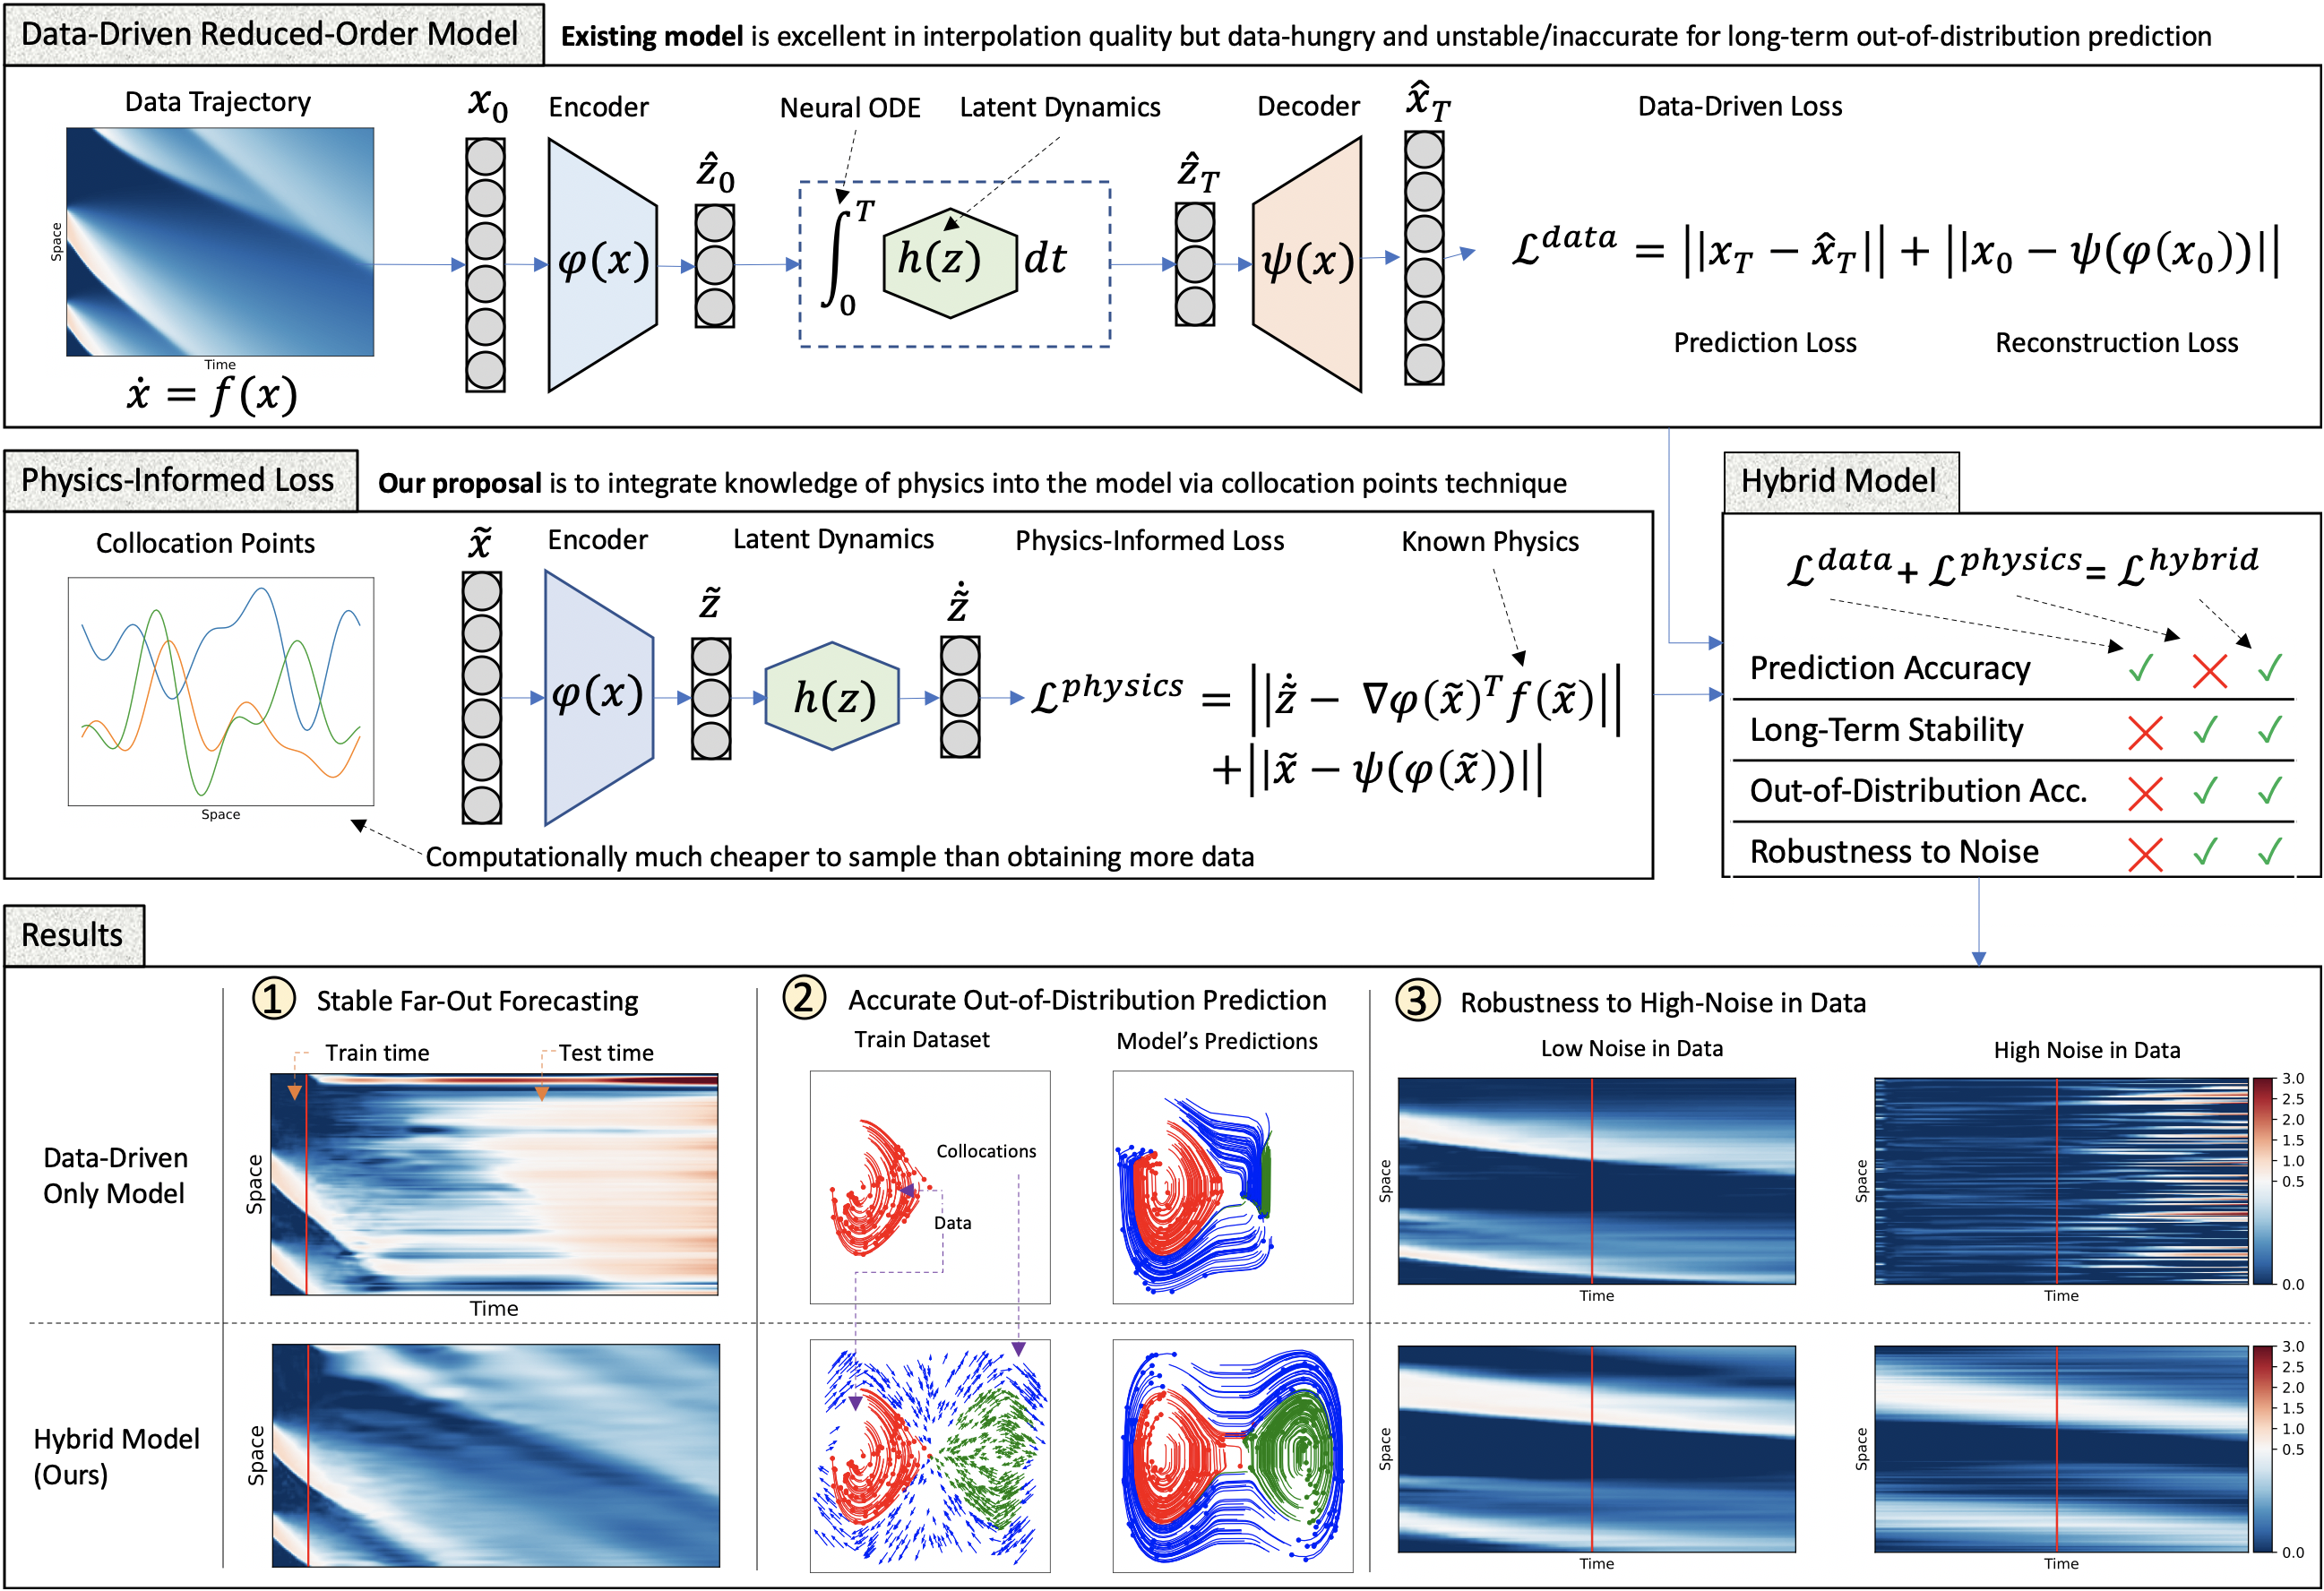
\includegraphics[width=\textwidth]{figures/graphical-abstract.png}
%    \caption{We propose utilizing a collocation points technique from numerical analysis to transfer knowledge of physics into continuous-time reduced-order models (ROMs). Such physics-informed models yield orders of magnitude more accurate predictions in tasks of far-out forecasting, predictions for out-of-distribution initial conditions, and learning from high-noise data. Good performance on those tasks is crucial for using ROMs in problems of compressive sensing and control.}
%    \label{fig:architecture}
%\end{figure}

\section{Methods}
\label{sec:method}
\paragraph{Reduced-Order Model with Non-Linear Latent Dynamics}
We consider an autonomous dynamical system on a finite space $\XX \subseteq \mathbb{R}^n$ given by

\begin{equation}
    \label{eq:generic_stationary_ode}
        \ddt\bd{x}(t) = \bd{f}(\bd{x}(t)).
\end{equation}

In real-world applications, it is often expensive to solve equation~(\ref{eq:generic_stationary_ode}) directly because $x(t)$ can be very high-dimensional. However, a variety of works provided both theoretical \citep{holmes2012turbulence} and empirical \citep{noack2011reduced,chen2021discovering} evidence that many physical systems evolve on a manifold $\ZZ \subseteq \mathbb{R}^m$ of a lower dimension $m << n$. In that space, the dynamics evolve according to a (generally unknown) function  $\bd{h}(\bd{z})$:

\begin{equation}
    \label{eq:latent_stationary_ode}
        \ddt\bd{z}(t) = \bd{h}(\bd{z}(t))
\end{equation}

We call the space $\XX$ an observable space, and $\ZZ$ a latent space. When an invertible mapping $\psi:\ \ZZ \to \XX$ between the observable and the latent spaces is known, one can predict the dynamics of the system $\bd{x}$ at a future time $T$ by projecting the initial condition $\bd{x}(0)$ into the latent space, integrating the dynamics in the latent space, and mapping the resulting trajectory back to the observable space:
\begin{equation}
\label{eq:integration_in_latent_space}
\begin{split}
    \bd{z}(0) & = \psi^{-1}(\bd{x}(0)) \\
    \bd{z}(T) & = \bd{z}(0) + \int_{0}^T\bd{h}(\bd{z}(t))dt \\
    \bd{x}(T) & = \psi(\bd{z}(T))
\end{split}
\end{equation}

When $m << n$ we refer to the triplet $(\psi, \psi^{-1}, \bd{h})$ as a Reduced-Order Model (ROM) of $\bd{f}$. It is often the case that for a given system $\bd{f}$, there exists no ROM $(\psi, \psi^{-1}, \bd{h})$ such that the relation~(\ref{eq:integration_in_latent_space}) holds exactly. In this case, we seek an \textit{approximation} ROM $(\psi_{\theta^*}, \phi_{\theta^*}, h_{\theta^*})$ that minimizes the difference between the data $x(t)$ and the prediction $\hat{x}(t)$ over a chosen class of models $(\psi_\theta, \phi_\theta, h_\theta)$ parameterized by $\theta$.

Multiple real-world applications necessitate using ROMs instead of integrating the relation~(\ref{eq:generic_stationary_ode}) directly. For example, integrating~(\ref{eq:generic_stationary_ode}) may be computationally intractable especially on platforms with limited computing capability such as embedded and autonomous devices. For instance, in an HVAC system, solving~(\ref{eq:generic_stationary_ode}) means solving a Navier-Stokes equation on a fine grid in real time, which exceeds the computing capabilities of current-generation appliances. On the other hand, integrating~(\ref{eq:integration_in_latent_space}) may be cheap when $m << n$. Finally, even when solving~(\ref{eq:generic_stationary_ode}) is possible in real time (e.g. by utilizing a remote cluster), executing control over the resulting model, which is an end-goal for an HVAC system, may still be intractable. Indeed, executing control requires \textit{multiple} evaluations of~(\ref{eq:generic_stationary_ode}) for \textit{each} iteration of control even for the most efficient algorithms known to date~\citep{duriez2017machine}. 

\begin{figure}
    \centering
    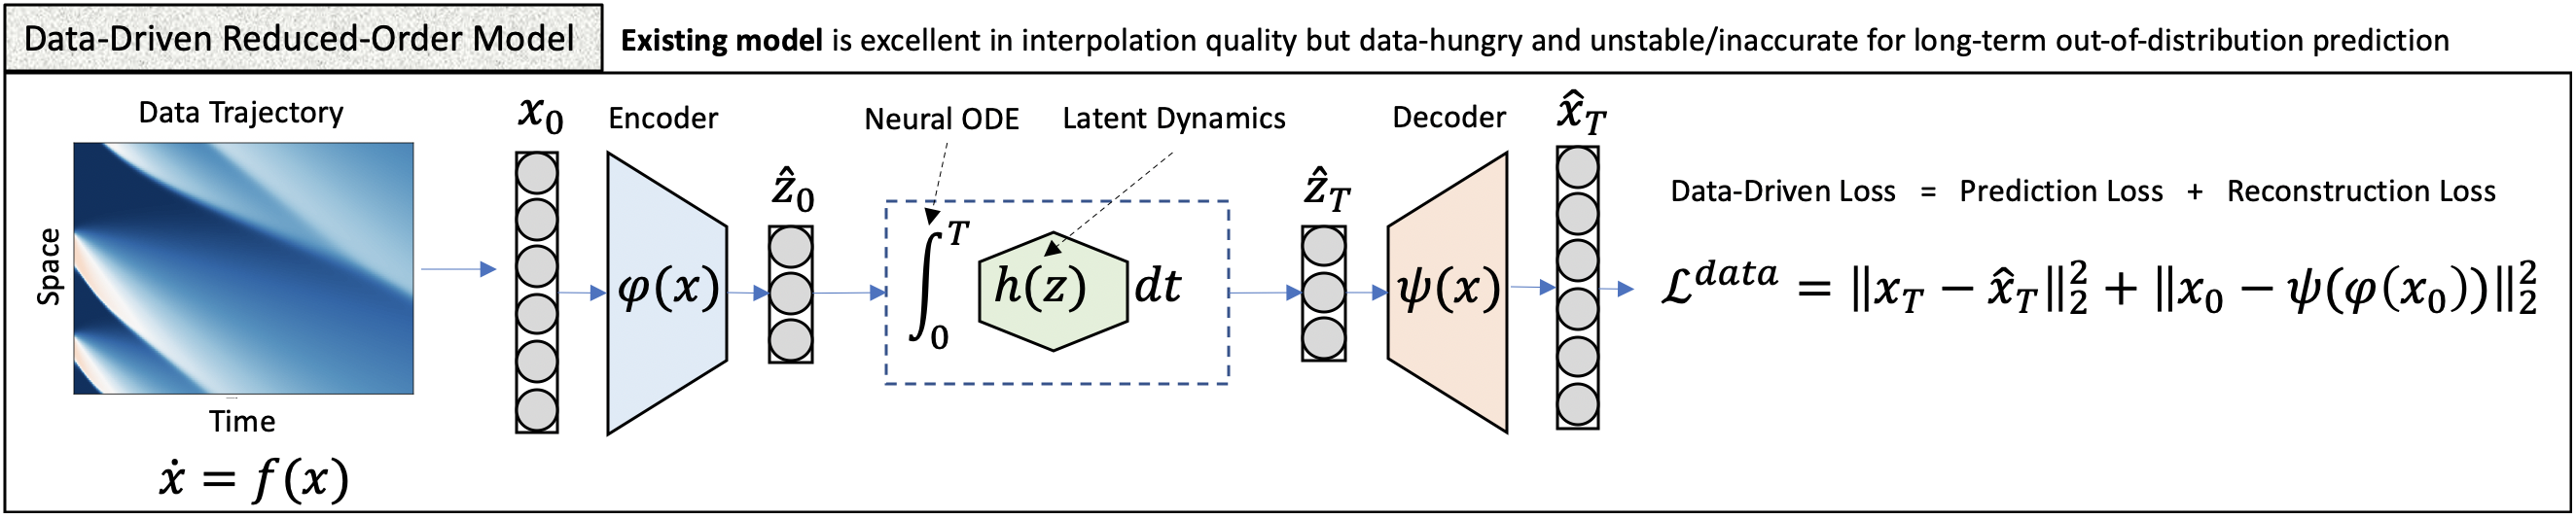
\includegraphics[width=\textwidth]{figures/abstract_data_driven.png}
    \caption{Illustration of the autoencoer structure with neural ODE in the latent space. The data-driven part of the loss function aims to minimize a sum of two objectives: the prediction loss and the reconstruction loss. The prediction loss minimizes the difference between the data trajectories and their model predictions to ensure temporal consistency of the latent space dynamics. The reconstruction loss ensures accurate reconstruction of individual snapshots, ensuring that the autoencoder behaves as an invertible mapping on all snapshots.}
    \label{fig:data_driven_loss}
\end{figure}

\paragraph{Architecture} In this work we model $\psi$, $\psi^{-1}$, and $\bd{h}$ with fully-connected neural networks $\psi_\theta$, $\phi_\theta$, and $h_\theta$, respectively. Specifically, the pair ($\psi$, $\psi^{-1}$) is modelled with an auto-encoder $(\psi_\theta, \phi_\theta)$, and $\bd{h}$ is modelled with a fully-connected network $h_\theta$. Figure~\ref{fig:data_driven_loss} visualizes the architecture of the model.

\paragraph{Data-Driven Loss} Similar to prior works \citep{takeishi2017learning,morton2019deep,gin2021deep}, we define a \textit{data-driven loss} $\LL_{data}$ as a sum of reconstruction and prediction losses. The former ensures that $\phi_\theta$ and $\psi_\theta$ are inverse mappings of each other, whereas the latter matches the model's predictions to the available data, as illustrated on Figure~\ref{fig:data_driven_loss}.

 Formally, for a given set of trajectories $\bd{x}_i$, $i \in [1 \dots k]$, where each trajectory $\bd{x}_i \in \mathbb{R}^{n \times p}$ is a set of $p$ snapshots that correspond to the recorded states of the system for $p$ time-steps, $t_j$, $j \in [1, \dots, p]$, the loss function $\LL^{data}_\theta$ is defined as:

\begin{align}
    \label{eq:loss_data_driven}
    \LL^{data}_\theta & = \frac{1}{2\sigma^2}\sum_{i = 1}^k \left[\frac{\omega_1}{p}\sum_{j=1}^p\left\|\bd{x_i}(t_j) - \psi_\theta(\phi_\theta(\bd{x_i}(t_j)))\right\|^2\right. + \\
     & + \left.\frac{\omega_2}{p}\sum_{j=1}^p \left\|\psi_\theta\left(\phi_\theta(\bd{x_i}(t_1)) + \int_{t_1}^{t_j}h(z(t))dt\right) - \bd{x_i}(t_j)\right\|^2 \right]
\end{align}
where $\sigma$ is the standard deviation of the observation noise. We note that each trajectory $\bd{x}_i$ may be captured over its own time-frame and may use a distinct, possibly non-uniform, step-size, in which case the loss function should be modified accordingly\footnote{The implementation is affected only in evaluating the integral in~(\ref{eq:loss_data_driven}). This part is handled by \texttt{torchdiffeq}~\citep{chen2018neural} library, which supports non-uniform time-frames within a batch}. To simplify the notation, without loss of generality, in the rest of the section we assume that all trajectories are recorded over the same time-frame with the same uniform step-size. To forecast the behavior of the system in the latent space, we apply the technique of Neural Ordinary Differential Equations (Neural ODEs or NODEs by~\citep{chen2018neuralode}, which utilizes the adjoint sensitivity method to back-propagate the gradients through the integral in~(\ref{eq:loss_data_driven}). Neural ODEs have demonstrated a better ability to model highly non-linear dynamics compared to linear models when the dimensionality of the dynamics variable is limited. This is especially useful in applications where the size of the latent space dimension needs to be small~\citep{lee2020model,gin2021deep,champion2019data,kim2019deep}.

\paragraph{Physics-Informed Loss} In their recent work, Liu et al.~\citep{liu2022physics} proposed a method for utilizing knowledge of the governing equations $d\bd{x}/dt = \bd{f(x)}$ as a finite-dimensional approximation of Koopman eigenfunctions for linear latent dynamics. To extend this approach to the non-linear regime, we note that for a true mapping $\phi$ the following holds:
\begin{equation}
    \label{eq:chain_rule_1}
    \frac{d\bd{z}(\bd{x}(t))}{dt} = \frac{d\bd{z}}{d\bd{x}}\frac{d\bd{x}}{dt} = \nabla\phi(\bd{x}(t))^T\bd{f}(\bd{x(t)})
\end{equation}
On the other hand, by the definition of $\psi$ and $\bd{h}$ we have that
\begin{equation}
    \label{eq:chain_rule_2}
    \frac{d\bd{z}(\bd{x}(t))}{dt} = \bd{h}(\phi(\bd{x}(t))
\end{equation}
Combining Equations~(\ref{eq:chain_rule_1}) and~(\ref{eq:chain_rule_2}) we get that
\begin{equation}
    \label{eq:physsics_informed_equation}
    \bd{h}(\phi(\bd{x}(t)) = \nabla\phi(\bd{x})^T\bd{f}(\bd{x})
\end{equation}

\begin{figure}
    \centering
    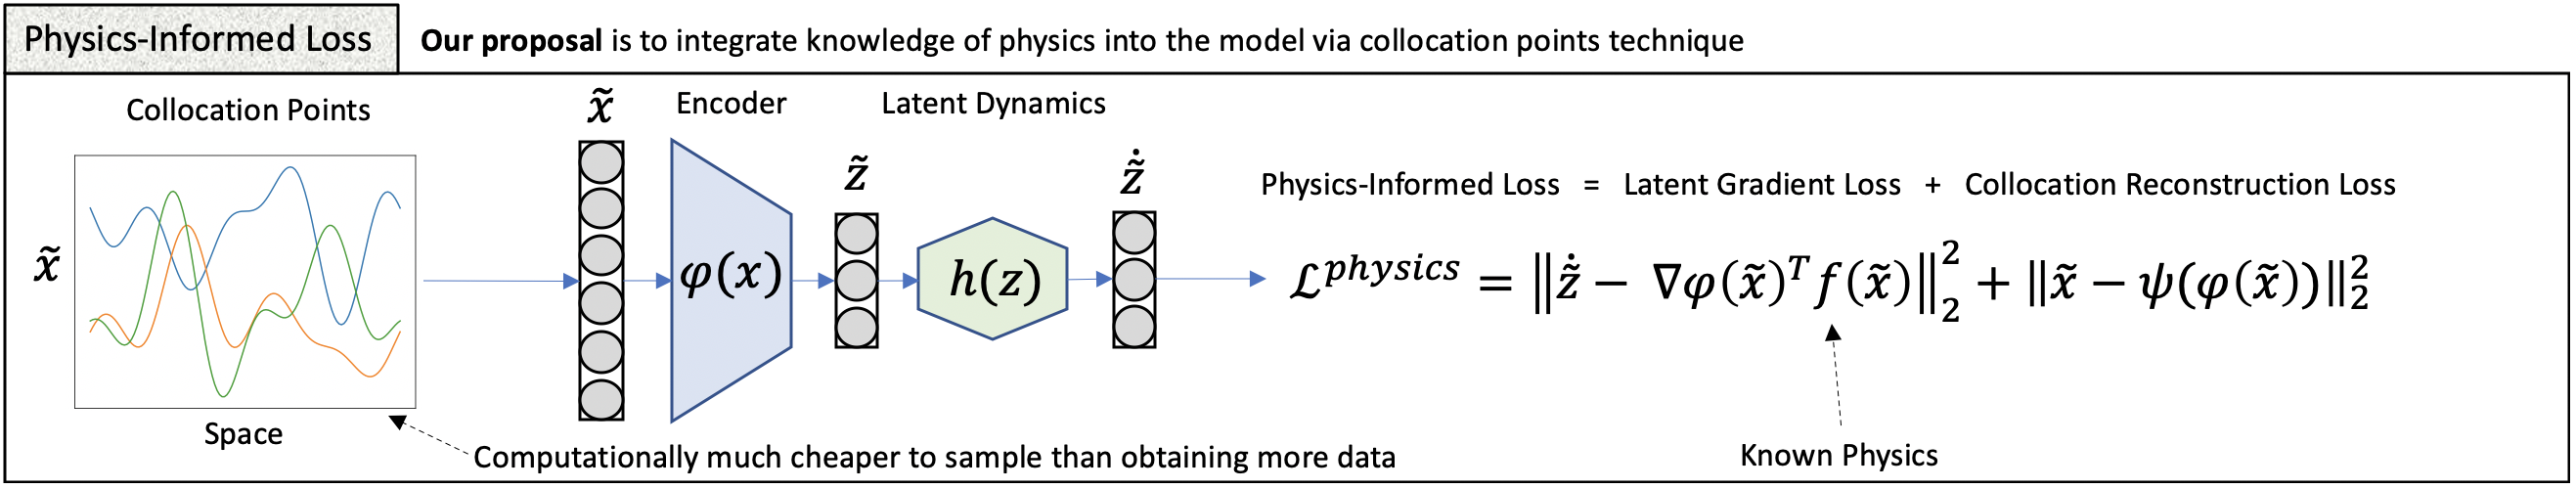
\includegraphics[width=\textwidth]{figures/abstract_physics_informed.png}
    \caption{The physics-informed loss function compares gradient fields in the current latent space with what a correctly-learned field should be in this latent space on set of collocation points.}
    \label{fig:physics_informed_loss}
\end{figure}

Equation~(\ref{eq:physsics_informed_equation}) links the dynamics $\bd{h}(\bd{z})$ and the encoder $\phi(\bd{x})$ with the known equation $\bd{f}(\bd{x})$ and is true for all $z \in \ZZ$ and $x \in \XX$. Hence, as shown on Figure~\ref{fig:physics_informed_loss}, knowledge of $\bd{f}$ can be assimilated into the model by evaluating Equation~(\ref{eq:physsics_informed_equation}) on a set of $N$ carefully sampled points $\bar{\bd{x}}_i \in \XX$, $i \in [1, \dots, N]$:

\begin{equation}
    \label{eq:loss_physics_informed}
    \LL^{physics}_\theta = \sum_{i = 1}^N \left[\frac{\omega_3}{N}\left\|h_\theta(\phi_\theta(\bar{\bd{x}}_i)) - \nabla \phi_\theta(\bar{\bd{x}}_i) \bd{f}(\bar{\bd{x}_i})\right\|^2 + \frac{\omega_4}{N}\left\|\bar{\bd{x}}_i - \psi_\theta(\phi_\theta(\bar{\bd{x}}_i))\right\|\right]
\end{equation}

We refer to the points $\bar{\bd{x}}_i$ as \textit{collocation points}.

\paragraph{Collocation Points}
\label{sec:collocations_conditions} We define a collocation as pair $(\bd{\bar{x}},\, \bd{f}(\bd{\bar{x}}))$. collocation points are samples from the space $\XX \times Im_{f}(\XX)$, and they should satisfy three conditions, ordered by importance:
\begin{enumerate}
    \item \textbf{Simplicity}: $\bd{f}(\bar{\bd{x}}_j)$ should be computationally cheap to evaluate. It is especially important for PDE systems, where $\bd{f}$ may involve high-order derivatives.
    \item \textbf{Representativeness}: $\bar{\bd{x}}_j$ should cover the space of states where one aims to improve the model's performance or stability. Collocation points that a model might encounter and that are not represented by data snapshots are the best candidates.
    \item \textbf{Feasibility}: $\bar{\bd{x}}_j \in \XX$. In other words, $x_j$ should be an attainable state of the system. Collocation points outside of $\XX$ may downgrade the performance of the autoencoder by forcing it to be an invertible function on a domain outside of $\XX$.
\end{enumerate}
Thus, an optimal sampling procedure for collocation points $\bd{\bar{x}}_j$ is domain-specific and should be designed given a particular system $\bd{f}$ and available data $\bd{x}_i$. We show examples of how these conditions can be implemented for real systems in the following sections.

The above definition of collocation points is not to be confused with a classic notion of collocation points for finding numerical solutions for differential equations~\citep{fornberg1998practical, trefethen2022numerical}. The classic notion refers to a set of points in time $[t_0, t_0 + c_1h, t_0 + c_2h, \dots, t_0 + h]$, $0 < c1 < c2 < \dots < 1$ which are chosen to obtain an optimal local interpolant of a solution of a differential equation for a time-period between $t_0$ and $t_0 + h$. For example, $s$ collocation points for Runge-Kutta methods are defined to provide an optimal Gauss-Legendre interpolant of order $s$; the coefficients $c_1, \dots, c_s$ come from a respective Butcher table. In contrast, we define collocation points as pairs $(\bd{\bar{x}},\, \bd{f}(\bd{\bar{x}}))$ which are  examples of mapping $x \to f(x)$. Our definition is built around solving an \textit{inverse} problem of approximating $\dot{x} = f(x)$ with $f_\theta(x)$ and follows a recent work~\citep{liu2022physics} which develops upon a definition from \citep{raissi2018hidden} with the difference being the sample space: instead of sampling from the spatiotemporal domain we sample them from an appropriate function space.

\paragraph{Combined Loss Function} We train the model by optimizing a sum of the physics-informed loss~(\ref{eq:loss_physics_informed}) and the data-driven loss~(\ref{eq:loss_data_driven}):
\begin{equation}
    \label{eq:loss_combined}
    \min_\theta \left[\LL^{physics}_\theta + \LL^{data}_\theta\right]  
\end{equation}
When $\omega_1 = \omega_2 = 0$ we have $\LL^{data}_\theta = 0$, so we say that the model is (purely) \textit{\textbf{Physics-Informed}}. Similarly, when $\omega_3 = \omega_4 = 0$ we have $\LL^{physics}_\theta = 0$ and we say that the model is (purely) \textit{\textbf{Data-Driven}}. When $\omega_i \neq 0, \, \forall i$, we say that the model is \textit{\textbf{Hybrid}}. 

The coefficients $\omega_i$ are hyper-parameters which need to be tuned using a validation dataset. However, in all experiments of this section we set $\omega_i$ to be either $0$ or $1$, and we balance $\LL^{physics}_\theta$ and $\LL^{data}_\theta$ the choice of samples in a batch of training data. Specifically, we set the number of collocation points per batch $N_{batch}$ to be equal to the number of trajectories per batch $k_{batch}$ times the number of time-steps$T$: $N_{batch} = Tk_{batch}$. In this way both $\LL^{physics}_\theta$ and $\LL^{data}_\theta$ represent the loss for $Tk_{batch}$ snapshots of the system, providing on average a similar contribution of information to the overall loss function. More laborious approaches of hyper-parameter tuning did not yield sufficient systematic advantage to justify the labour compared to this simple strategy.

We use a \texttt{pytorch}~\citep{NEURIPS2019_9015} implementation of the Adam algorithm~\citep{kingma2014adam} for optimization. To evaluate $\nabla_\theta \LL^{physics}_\theta$ and $\nabla_\theta \LL^{data}_\theta$ we use \texttt{torchdiffeq}~\citep{chen2018neural} -- a \texttt{pytorch}-compatible implementation of the Neural ODE framework. 

To the best of our knowledge, this is the first framework that combines non-linear latent-dynamics (Neural ODE), autoencoders, and a physics-informed loss term~(\ref{eq:loss_physics_informed}). Thus, we call our framework \textit{Physics-Informed Neural ODE}, or PINODE. 
\begin{figure}[t]
    \centering
    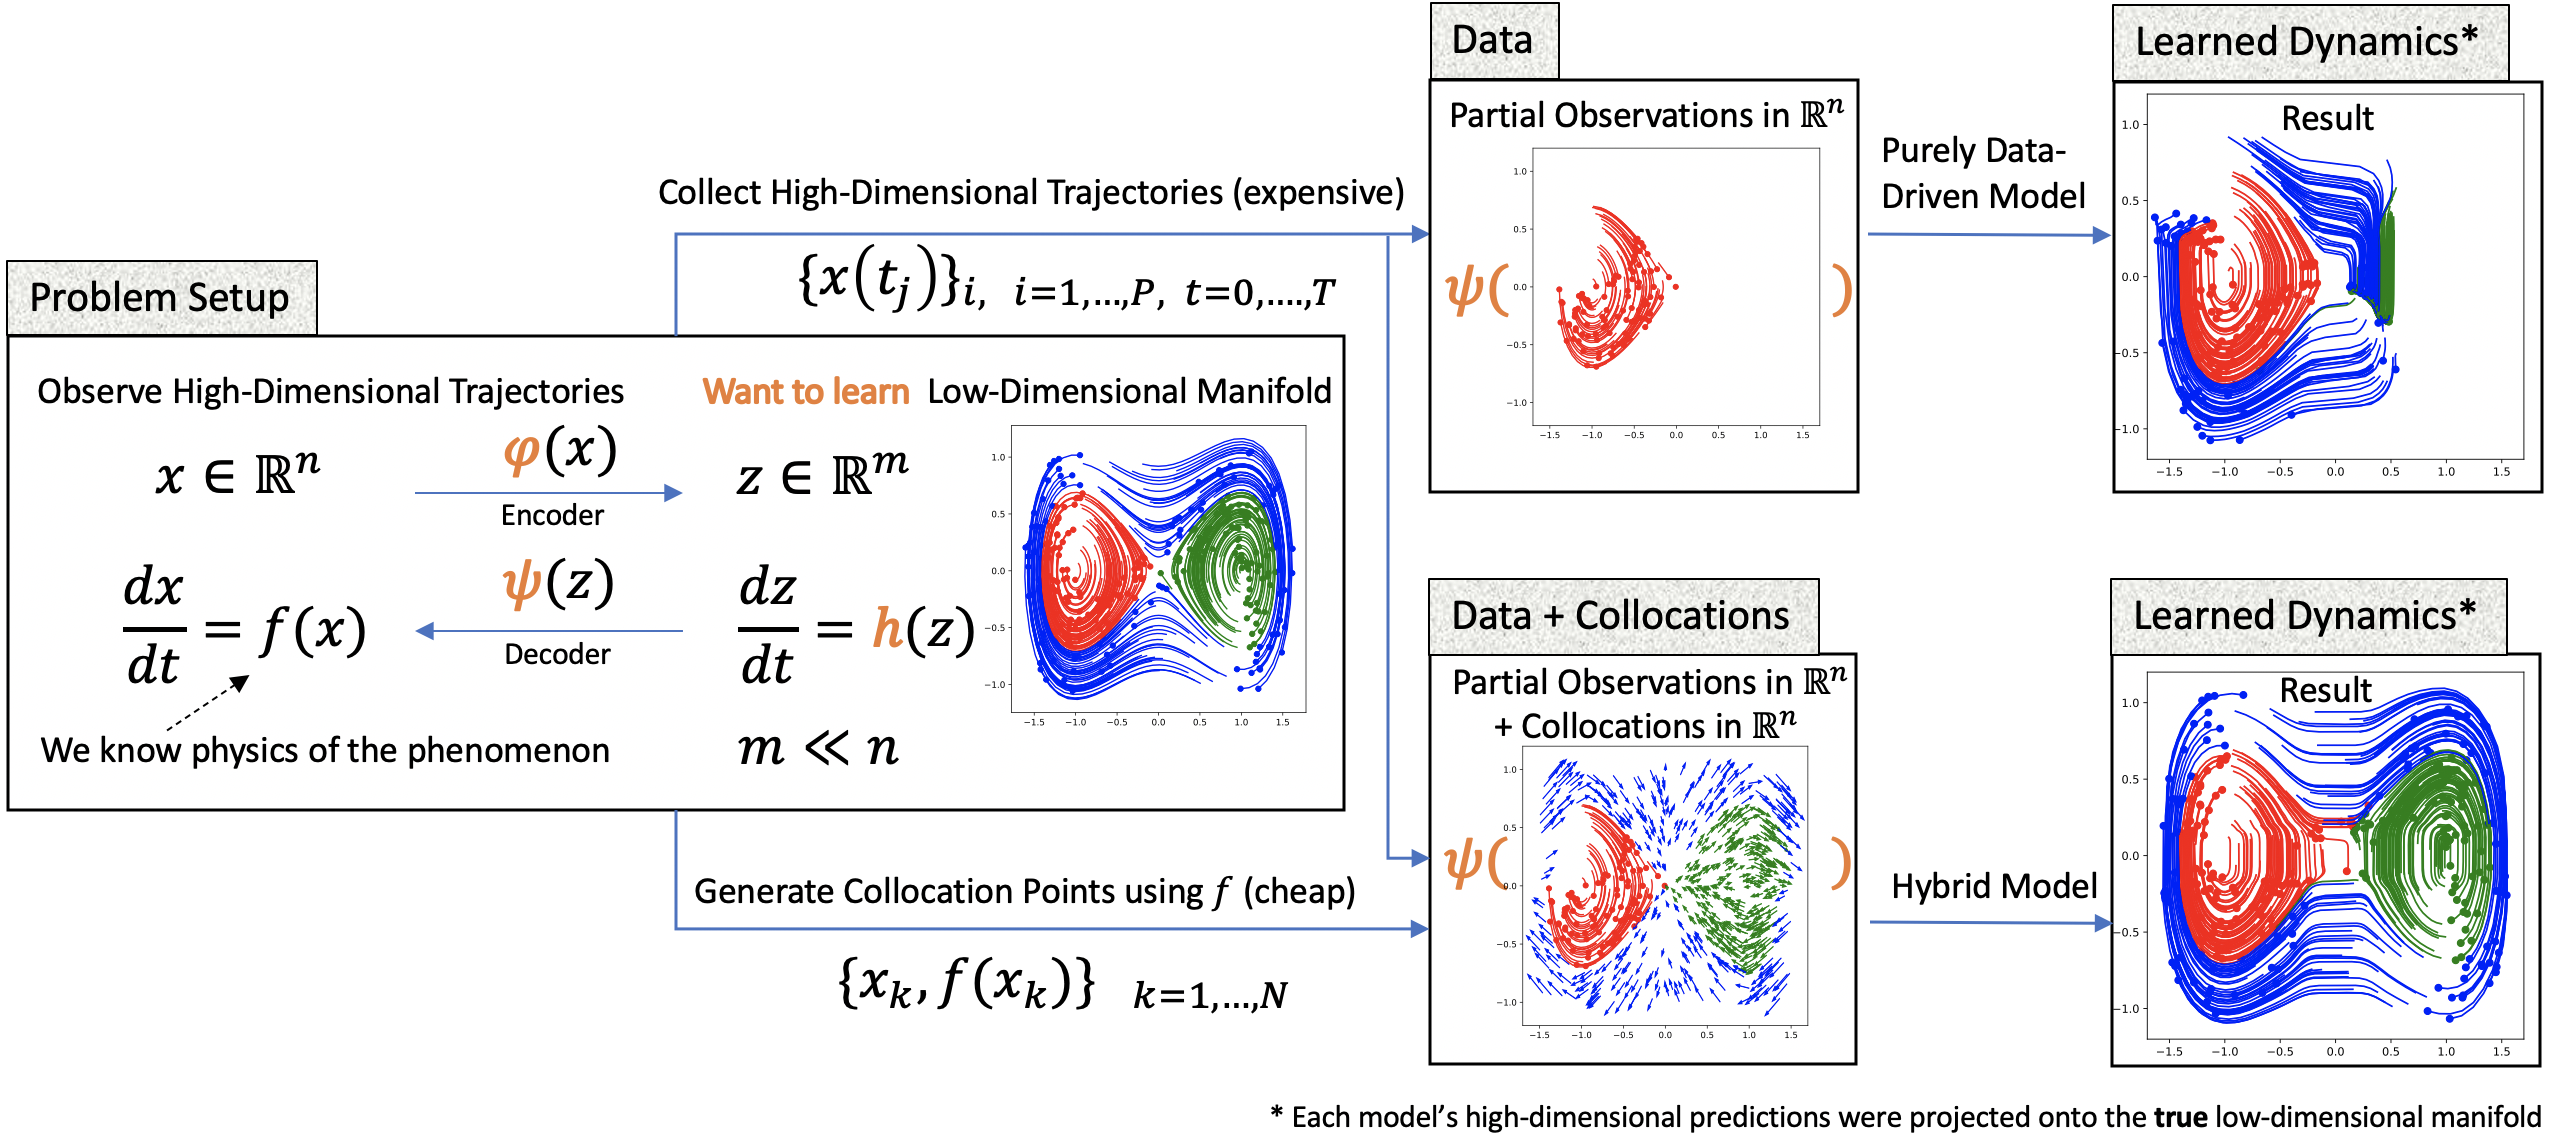
\includegraphics[width=\textwidth]{figures/duff_first_exp_abstract.png}
    \caption{We use a toy example -- a Lifted Duffing Oscillator -- to show that it is possible to ``fill the gaps'' in data with collocation points. Specifically, the Hybrid model is able to learn the dynamics of two additional basins of attraction that were not represented in the dataset. As shown in the top-rightmost frame, without the collocation points the model does not infer the dynamics in the unseen regions correctly.}
    \label{fig:duffing_pinode}
\end{figure}

\section{Experiments}
\label{sec:exp}
The experiments section is organized as follows. First, to illustrate the ideas behind the framework we study its performance on a high-dimensional ODE -- a lifted Duffing oscillator. We show how a non-linear latent dynamics $\bd{h}(\bd{z})$ overcomes the limitations of DMD and Koopman networks from \citep{liu2022physics} by handling multiple basins of attraction within one model. We also show that using physics-informed loss is sufficient for reconstructing the behaviour for basins of attraction that are not represented by the data. Finally, we demonstrate that a purely data-driven model may be highly-accurate in the short-term and highly unstable in the long-term, even when the data is abundant, and show that the physics-informed approach improves long-term stability of such models by multiple orders of magnitude.

Next, we study the framework's performance on Burgers' equation. We show that (i) the non-linear latent dynamics model yields more compact latent space representations than its linear counterpart for the same accuracy; (ii) the compact latent space representations allow for more stable long-term predictions; (iii) in the presence of significant noise in the data, the use of collocation points improves stability by providing an extra source of information that is noise-free, and (iv) in certain scenarios, training \textit{only} on collocation points yields \textit{better} models than training on data, even when a vast amount of data is available. The last observation shows that the contribution of the physics-informed loss~(\ref{eq:loss_physics_informed}) may surpass that of the data-based loss~(\ref{eq:loss_data_driven}), especially when the data is severely limited or noisy. 



\subsection{Lifted Duffing Oscillator}
\label{sec:duffing}

A Duffing oscillator is a dynamical system $d\bd{z}/dt = \bd{h}(\bd{z})$ such that 

\begin{equation}
    \label{eq:duffing_definition}
    \begin{split}
    \frac{dz_1}{dt} & = z_2 \\ 
    \frac{dz_2}{dt} & = z_1 - z_1^3
    \end{split}
\end{equation}

A phase portrait for 300 randomly sampled trajectories from this system is visualized on Figure~\ref{fig:duffing_pinode}, left frame. Depending on the total energy, each trajectory always stays in one of three regions: the left lobe, the right lobe, or the outer area, visualized in red, green, and blue, respectively. To create a synthetic high-dimensional system that retains this property, we lift the Duffing trajectories into a higher-dimensional space by applying an invertible transformation~$\mathcal{A}(\bd{z})$: 

\begin{figure}
  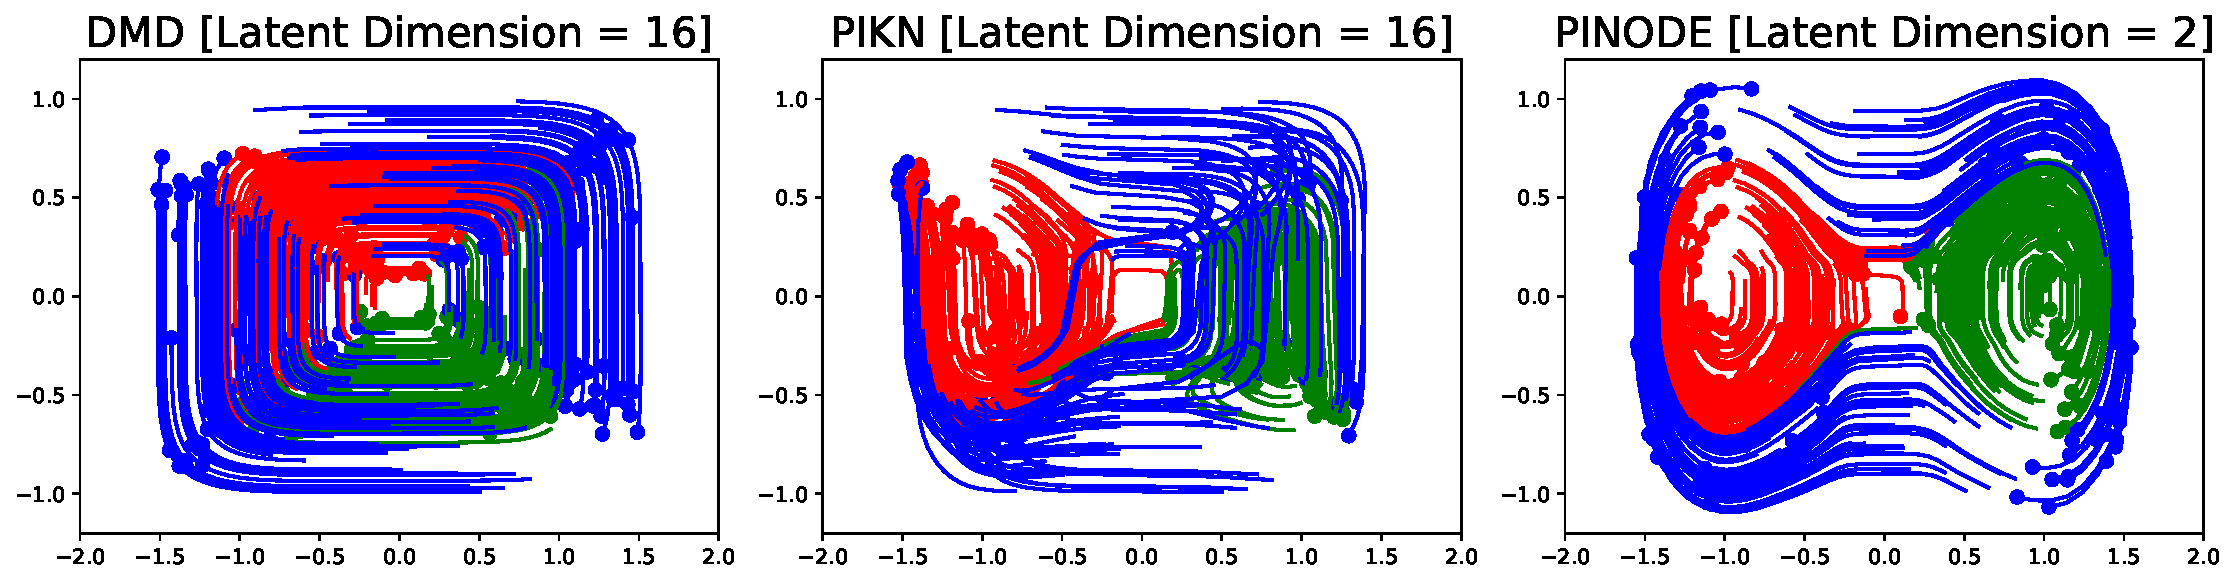
\includegraphics[width=\textwidth]{figures/duffing_comparison.pdf}
  \caption{\label{fig:duffing_comparison}Non-linearity in the latent dynamics and the autoencoder employed in teh PINODE Hybrid model are important for accurate long-term extrapolation. The DMD model and PIKN Hybrid model were unable to extrapolate the dynamics from collocation points.}%\vspace{-0.5in}
\end{figure}

\begin{equation}
    \label{eq:duffing_true_decoder}
    \bd{x} := \mathcal{A}(\bd{z}) = A\bd{z}^3, \quad A \in \mathbb{R}^{128 \times 2}, \quad A_{ij} \sim_{i.i.d.} \mathcal{N}(0, 1)
\end{equation}


Hence, for this system $z \in \ZZ = \mathbb{R}^2$ and $\bd{x} \in \XX = \text{span}\{A_{:,1}, A_{:,2}\} \subseteq \mathbb{R}^{128}$. We treat $\XX$ as an observable space, in which the dynamical system~(\ref{eq:duffing_definition}) obeys the following:
\begin{equation}
    \frac{d\bd{x}}{dt} = \bd{f}(\bd{x}) = \nabla((A^TA)^{-1}A^T\bd{x}^{1/3})^T\bd{h}((A^TA)^{-1}A^T\bd{x}^{1/3})
\end{equation}

Thus, we created a high-dimensional dynamical system with multiple basins of attraction for which the dynamics $\bd{f}$ are known.

For the experiment, we generate 6144 trajectories $\bd{x}_i$, $t=[0, 1]$, $\Delta t = 0.1$, all taken from the left lobe region (in red). We also sample 50000 collocation points $\bar{\bd{x}}_j$ from the right (green) and the outer (blue) regions each by sampling $\bar{\bd{z}}_j \in U\left([-3/2,\, 3/2] \times [-1, 1]\right)$ and then applying the transformation~(\ref{eq:duffing_true_decoder}). For this example the conditions for collocation points discussed in Section~\ref{sec:method} are trivially satisfied.


We train two PINODE models: a Data-Driven model that only uses the trajectories, and a Hybrid model that uses both trajectories and collocation points. The models share the same architecture and training parameters that are detailed in Appendix~\ref{appendix:duffing_pinode}. After training, we invert the mapping~(\ref{eq:duffing_true_decoder}) to project the models' high-dimensional predictions for unseen initial conditions onto the true low-dimensional manifold; those are visualized in  Figure~\ref{fig:duffing_pinode}.  




We make two observations from the results displayed in Figure~\ref{fig:duffing_pinode}. First, a purely data-driven model is unable to extrapolate outside its training region using only the data from that region. This observation is consistent with the conclusions from related works~\citep{gin2021deep} that neural networks interpolate well but struggle with extrapolation tasks. Second, we see that collocation points provided enough extra information for the model to predict nearly perfectly in regions from which no trajectories were provided. This observation suggests that one can use collocation points to ``cover the gaps'' in data and improve the extrapolation accuracy of the model. 
\begin{figure}[t]
    \centering
    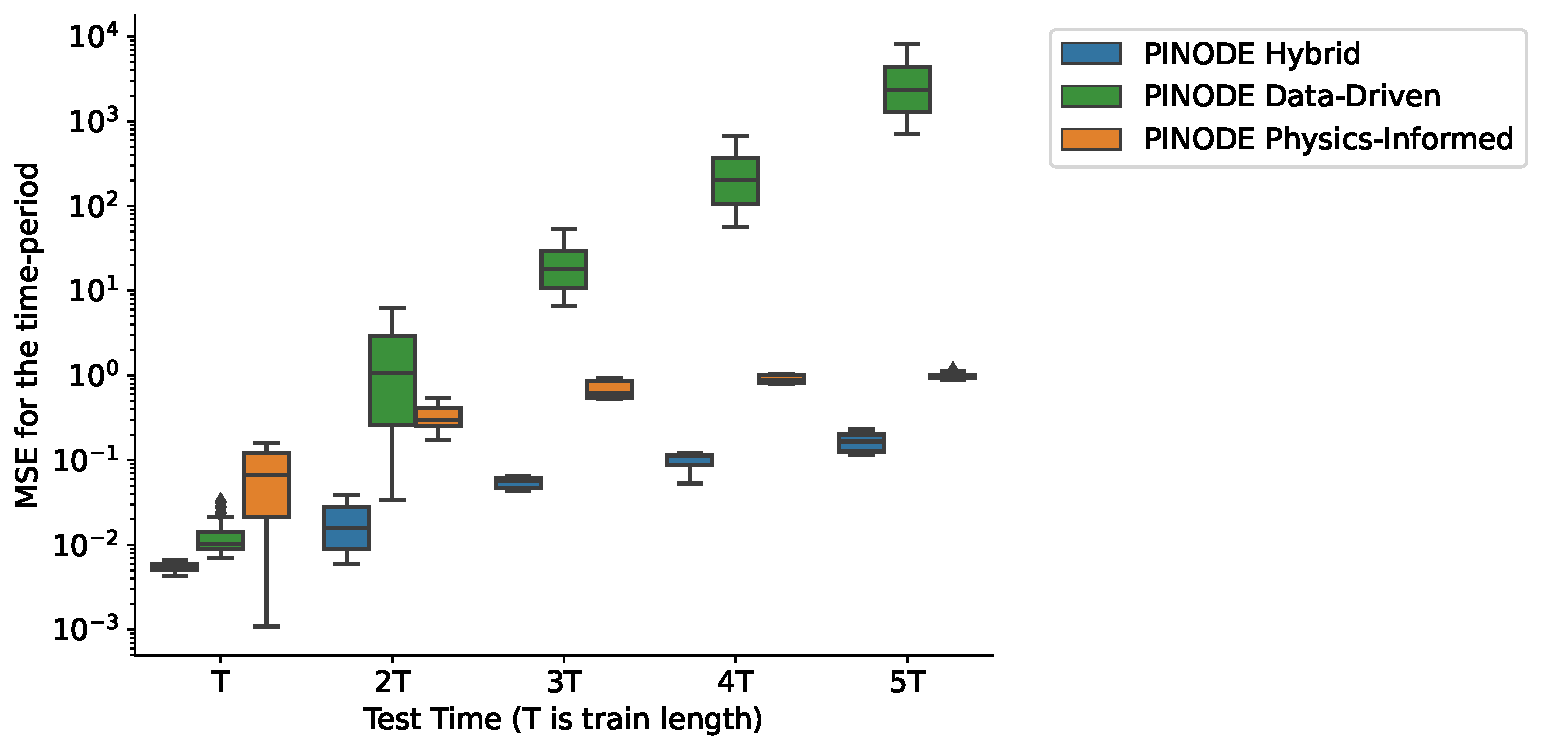
\includegraphics[width=0.7\textwidth]{figures/duffing_periods.pdf}
    \caption{ Box plots of the prediction error for three PINODE models: Data-Driven, Physics-Informed, and Hybrid. The time is measured in multiples of the training time period, i.e. $x=3T$ refers the time-range between two and three training time-periods away. }%\vspace{-0.4in}
    \label{fig:duffing_periods}
\end{figure}


The ability of Neural ODE to model nonlinear dynamics in the latent space is demonstrated in Figure~\ref{fig:duffing_comparison}. The figure shows a comparison between the Hybrid PINODE model, the Hybrid PIKN model~\citep{liu2022physics}, and DMD, all of which have been trained using the same dataset. PIKN differs from PINODE in that it uses linear latent dynamics $\frac{dz}{dt} = Lz$, where $L$ is a finite-dimensional approximation of the Koopman operator, instead of a general non-linear dynamics operator $\frac{dz}{dt} = h_\theta(z)$. For PIKN, we set $z \in \mathbb{R}^{16}$, an 8 times expansion of the dimension of the true manifold. We observe in Figure~\ref{fig:duffing_comparison} that PIKN is unable to extrapolate the dynamics to unseen areas correctly using the collocation points: eventually, all trajectories "collapse" onto the same attractor. It can also be seen that DMD shows even worse performance which could be attributed to its linear model reduction.

In the next experiment, we show that collocation points stabilize long-term predictions of the model even when data from all parts of the space are available. To illustrate, we generate a dataset of 6144 trajectories (2048 trajectories per red, green, and blue area) and 50000 collocation points uniformly distributed among all three lobes. We train three models: Data-Driven, Physics-Informed, and Hybrid versions of PINODE. The relative performance of the three models is evaluated in Figure~\ref{fig:duffing_periods}, where the x-axis represents the test time-horizon as multiples of the training trajectory length $T$. The $y$-axis shows box plots of the prediction mean squared error (MSE) corresponding to 300 unseen trajectories within the specific period. For example, $x = 2T$ represents the time-period $[2T, 3T)$, and the $y$-axis shows the distribution of the prediction errors within the period $[2T, 3T)$. Figure~\ref{fig:duffing_periods} shows that the performance of the Data-Driven model degrades quickly when the forecasting time-period increases despite its excellent performance when forecasting within its training time-period. The Physics-Informed model starts with modest performance over the training time horizon but maintains a stable performance when forecasting far ahead. The Hybrid model, in its turn, combines both near-term accuracy with long-term stability, yielding the best results over each time period. 

\subsection{Burgers' equation}
\label{sec:burger_eqn}
We now study the performance of our framework on Burgers' equation with $[-\pi, \pi]$-periodic boundary conditions:
\begin{equation}
\begin{split}
\label{eq:burgers_equation}
    & u_t  + uu_x = \nu u_{xx} \\
    & u(-\pi, t) = u(\pi, t),\quad \forall t \in [0, T]
\end{split}
\end{equation}
where $u_t$, $u_x$, and $u_{xx}$ represent partial derivatives in time, the first, and second spatial derivatives, respectively. Burgers' equation is a PDE occurring in applications in acoustics, gas and fluid dynamics, and traffic flows \citep{burgers1948mathematical}. When $\nu$ is significantly smaller than one, the system exhibits strong non-linear behaviour and is called ``advection-dominated'', otherwise when $\nu$ is large the system is called ``diffusion-dominated''. 
In the case of the former, linear projection methods such as POD become inaccurate as the true solution space has a slow decaying Kolmogorov n-width, manifesting itself in slow decaying singular values \citep{peherstorfer2022breaking}. Therefore, in this section we focus on the advection-dominated Burgers' equation for which we set $\nu = 0.01$.


To generate trajectories, we discretize the spatial domain $[-\pi,\,\pi]$ into 128 grid-points, and solve Equation~\ref{eq:burgers_equation} for $t \in [0, 2]$ with $\Delta t = 0.1$ using a spectral solver~\citep{trefethen2000spectral}. To generate a diverse set of initial conditions we sum the first 10 harmonic terms with random coefficients:
\begin{equation}
    \label{eq:burger_initial_condition}
    u(x, 0) = \frac{1}{10}\sum_{k = 1}^{10} a_k\cos(kx) + b_k\sin((k+1)x), \quad a_k, b_k \sim \mathcal{N}(0, 1)
\end{equation}

To generate collocation points we use the same family of functions as we used for the initial conditions in Equation~(\ref{eq:burger_initial_condition}), and additionally randomize the presence of individual frequencies in the sum:
\begin{equation}
    \label{eq:burger_collocations}
    \bar{u}(x) = \frac{1}{10}\sum_{k = 1}^{10} p_ka_k\cos(kx) + q_kb_k\sin((k+1)x), \quad a_k, b_k \sim \mathcal{N}(0, 1), \quad p_k, q_k \sim Be(1/2).
\end{equation}
We choose this family of collocation points to meet the conditions~(\ref{sec:collocations_conditions}). First, this family is representative of the state space $\XX\times Im_f(\XX)$ in the region of interest (moving wave-fronts). Second, (\ref{eq:burger_collocations})~is a smooth set of functions that does not contain unattainable states. Finally, and more importantly, the values $u_x$ and $u_{xx}$ and, consequently $u_t$ can be computed analytically, which makes it especially cheap to sample large numbers of collocation points. 

\subsection{Compressibility of the Latent Space}


\label{sec:compressibility}
\begin{figure}[t]
    \centering
    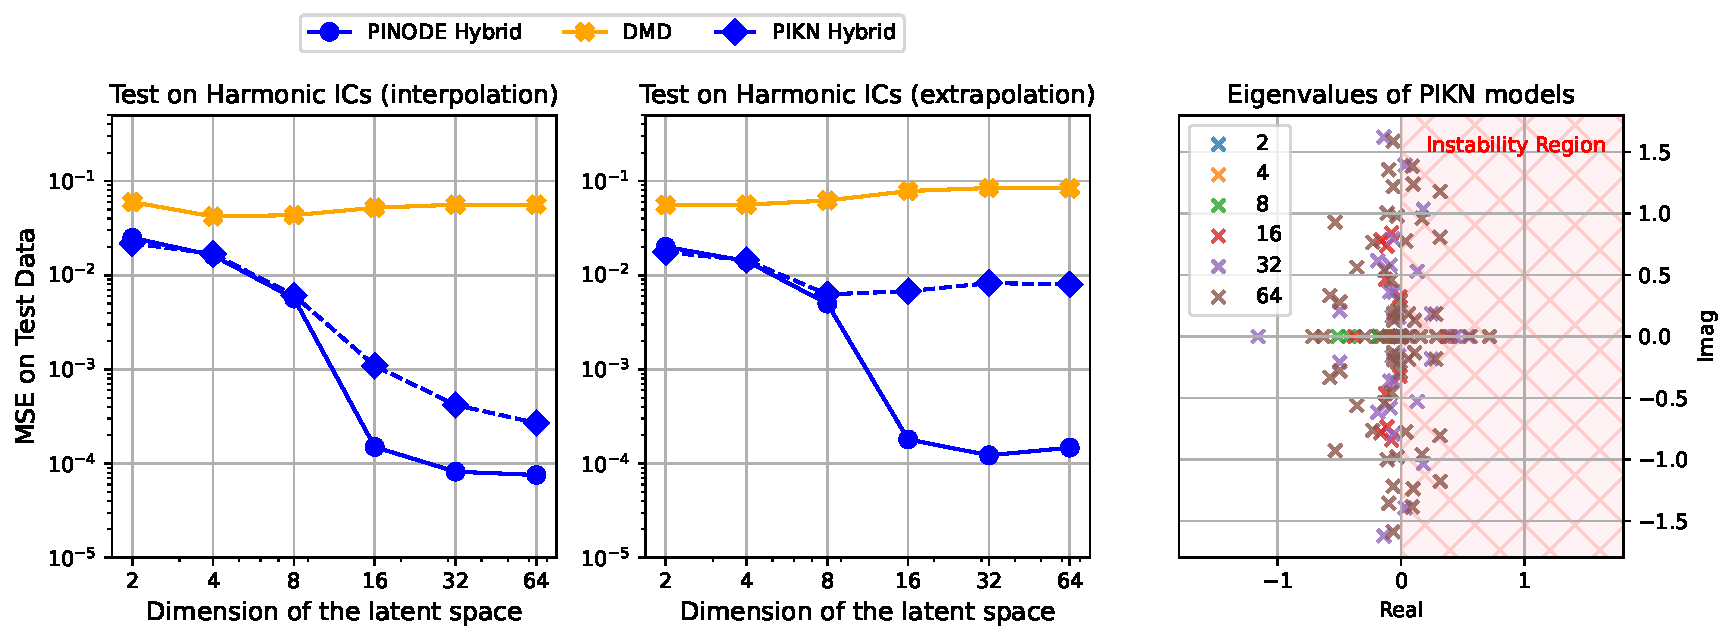
\includegraphics[width=\textwidth]{figures/compressibility.pdf}
    \caption{PINODE Hybrid model utilized the latent space dimension 5 times more efficiently in terms of MSE than PIKN Hybrid model when modelling low-viscosity (highly-nonlinear) Burgers' equation (left frame). The difference in performance grows to x100, when forecasting two times farther than the training period (central frame). PIKN suffers from long-term instability due to the presence of eigenvalues with positive real part in the latent dynamics matrix (right frame). In this frame we plot all the eigenvalues of the latent-space matrix for each PIKN model from frames 1-2. The legend in the right frame refers to the dimension of the latent space used by the corresponding PIKN model.}
    \label{fig:burgers_compressibility}
\end{figure}

In Section~\ref{sec:duffing}, we showed that a non-linear finite-dimensional latent dynamics model can be necessary for building a compact ROM for the high-dimensional lifted Duffing system. That is \textit{not} necessarily the case for Burgers' equation since there exists the Cole-Hopf transformation that linearizes the dynamics for Burgers' equation. However, a latent-space non-linearity can, in principle, be utilized for finding a more compact latent space representation, or for increasing the forecast accuracy for a fixed latent space dimension. In this section, we demonstrate how PINODE can achieve both goals. 

For this experiment we generate 16384 trajectories as described in~(\ref{eq:burger_initial_condition}). We also generate 100000 collocation points as described in~(\ref{eq:burger_collocations}). The purpose of using such a large amount of data is to allow the trained models to achieve the best performance for the specified latent space dimension. We evaluate the performance of the models on test data with two different time-frames: (1) same as that of training data (\textit{interpolation}), and (2) two times longer than that of the training data (\textit{extrapolation}). More details on the experimental setup are provided in Appendix~(\ref{appendix:burgers_compressibility}).

In Figure~\ref{fig:burgers_compressibility}, we compare the performance of the three models: DMD, PIKN Hybrid, and PINODE Hybrid. First, we notice that DMD does not perform well on the test data, despite achieving a training loss ($\sim 10^{-3}$). This observation is consistent with earlier works~(\citep{kalur2021robust,kutz2016dynamic}); and illustrates well that a combination of a linear encoder and a linear latent dynamics operator may not be sufficient for modelling highly-nonlinear phenomena. Second, we notice that PINODE achieves better performance for a given latent space dimension compared to PIKN. For instance, for $m = 16$ (Figure~\ref{fig:burgers_compressibility}, left pane), PINODE achieves $\sim 5$ times lower mean squared error than PIKN, which achieves the same performance only when $m = 512$. More importantly, PINODE maintains a low prediction error over a longer-term horizon (extrapolation in time), which is not the case for PIKN (Figure~\ref{fig:burgers_compressibility}, center pane). This is a consequence of the latent-dynamics matrix ($h(z) = Lz$) of PIKN having eigenvalues with positive real parts, which implies long-term instability (Figure~\ref{fig:burgers_compressibility}, right pane). Although there has been progress in the literature~\citep{kojimalearning}, further research is needed to understand (i) how to enforce stability constraints for PIKN, and (ii) why one does not need the same enforcement for PINODE to exhibit stable behaviour. 

	\begin{figure}[t]
        \centering
        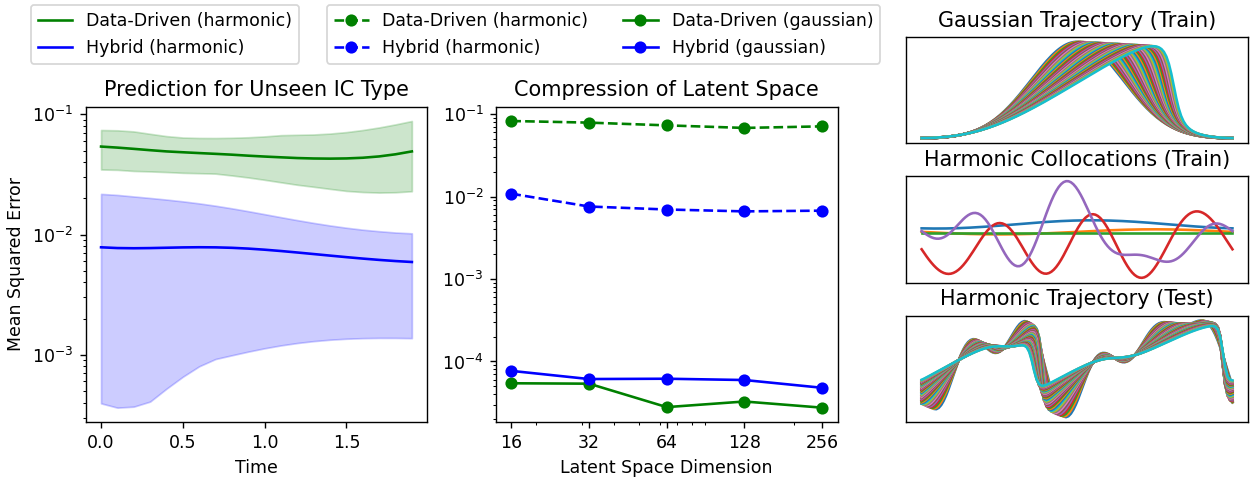
\includegraphics[width=\textwidth]{figures/burgers_compression.png}
        \caption{The right plots give examples of data snapshots used: trajectories with bell-curve ICs (top) and harmonic ICs (bottom). The middle-right pane shows harmonic collocations used by hybrid models in addition to the snapshots. The left plot compares the prediction errors (MSE) of two models, data-driven and hybrid with 128-dimensional latent spaces, on harmonic initial conditions that were not present in the trained data. The shaded regions represent 95\% confidence intervals based on 100 test trajectories. The middle plot shows the prediction error (MSE) on each type of test data for a variety of models with different latent-space sizes. We see that the use of harmonic collocations significantly improves the model performance on unseen harmonic ICs without increasing the errors on bell-curve ICs.}
        \label{fig:pikn_burgers_compression}
    \end{figure}
    
However, we observe that PIKN benefits from using physics-informed loss as well. In particular, we show that one can use collocations to improve model's performance on types of initial conditions that are missing in the available training data. To illustrate that we train two models. The data-driven model only uses 1024 trajectories with bell-curve initial conditions (ICs) (we provide an example at the top-right frame of the Figure~\ref{fig:pikn_burgers_compression}). The hybrid model additionally observes 80000 harmonic collocations formed by summing first 10 sinusoidal modes with random coefficients (Figure~\ref{fig:pikn_burgers_compression}, middle-right frame), for which we evaluate $u_t$ analytically using Equation~\ref{eq:burgers_equation}. Next, we evaluate the performance of both models using unseen trajectories with both harmonic and bell-curve ICs, 100 trajectories each. We observe that the Hybrid model predicts the sinusoidal trajectories ~10 times better than the data-driven one (Figure~\ref{fig:pikn_burgers_compression}, left frame, shown for the 128-dimensional latent-space model). Since neither models had any trajectories of that type in its training set we conclude that the difference in performance comes from using harmonic collocations. We also note that better performance of the hybrid model on harmonic ICs does not come at an expense of worse performance on bell-curve ICs, as shown in the central frame of Figure~\ref{fig:pikn_burgers_compression}. This evidence suggests that one can improve a model's extrapolation power  by supplementing its training with sufficiently diverse set of collocations, especially when additional simulations are expensive to obtain but the collocations are cheap to generate. The details of the network's architecture and training procedure are provided in the Appendix \ref{appendix:pikn_burgers}.


\subsection{Training in Low-Data Regime with Collocation Points}
\label{sec:data_vs_collocations}

In the next experiment, we study the relative efficiency of using collocation points against using data in a low-data regime. It is frequently the case that only a small number of simulations (or measurements) can be obtained for a physical system of interest due to the computational, time, or budget constraints. We would like to compensate the lack of sufficient data with providing collocation points which are considerably cheaper to generate. In this section, we show that, when chosen appropriately, collocation points can be effectively used for training a model in the low-data regime, and their contribution to a model's accuracy may even surpass the contribution of the data. 
\begin{figure}[t]
    \centering
    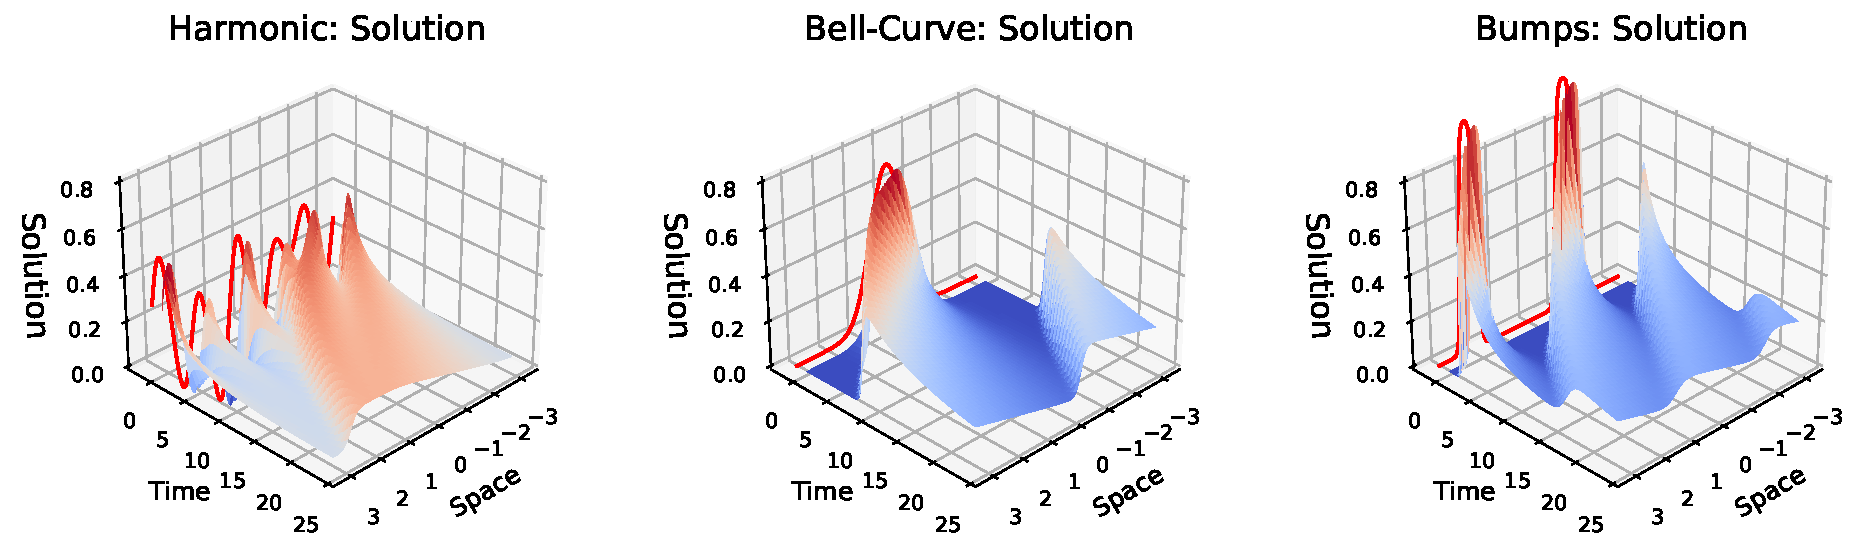
\includegraphics[width=0.8\textwidth]{figures/burgers_examples_of_ics.pdf}
    \caption{Examples of "harmonic", "bell-curve", and "bump" initial conditions, as well as the resulting solutions, in columns 1, 2, and 3, respectively.}
    \label{fig:burgers_examples_of_ics}
\end{figure}

To illustrate the trade-off between data and collocations, we train one model using varying combinations of the number of trajectories vs collocation points in their training datasets. To gauge the extrapolation power of our models, we use trajectories with three types of initial conditions: ``harmonic'', ``bell-curve'', and ``bumps'' (see Figure~\ref{fig:burgers_examples_of_ics} for illustrations). We generate 1024 trajectories with ``bumps'' initial conditions for the training data, and use the harmonic family of initial conditions as described in~(\ref{eq:burger_collocations}) for generating the training collocations. We use two test datasets: (1) 100 trajectories with ``bump'' ICs to assess within-distributuion performance, left frame), and (2) a mix of trajectories with ``bump'', ``bell-curve'', and ``harmonic'' initial conditions, 100 trajectories each, to assess out-of-distribution performance. All test data trajectories are two times longer than the training trajectories. More details on the experimental setup are provided in Appendix~\ref{appendix:burgers_data_vs_collocations}. Figure~\ref{fig:burger_data_vs_collocations} presents the reconstruction MSE of the test datasets obtained from a PINODE models that were trained on varying combinations of trajectories and collocation points as a percentage of the MSE achievable by a PINODE model that was trained on the full 1024 trajectories alone (no collocations). The PINODE models all use a latent space dimension $m=16$. 

\begin{figure}[t]
    \centering
    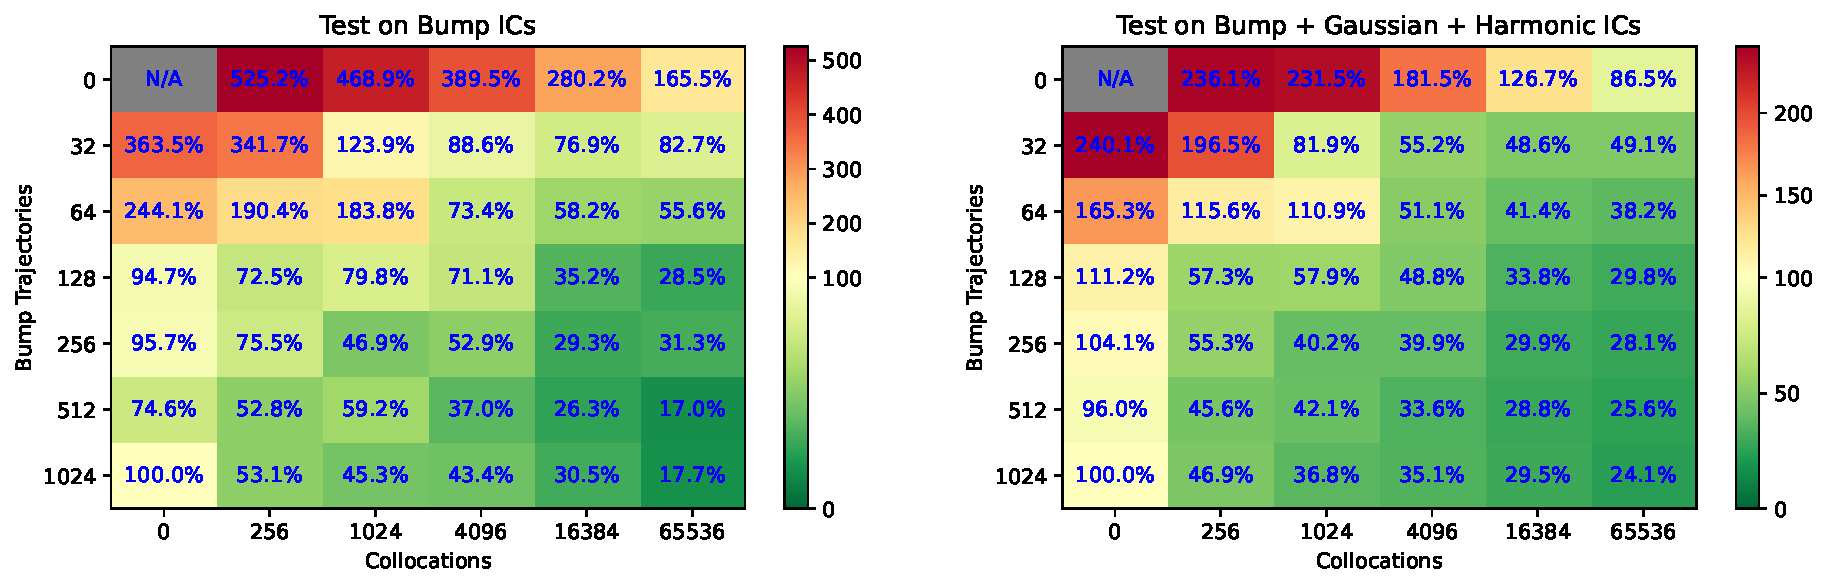
\includegraphics[width=0.9\textwidth]{figures/data_vs_collocations.pdf}
    \caption{Comparison of the achievable MSE relative to the full data regime (1024 trajectories). When the data is scarce, collocations-based physics-informed loss improves the forecasting accuracy of ROMs by an average of 5 times lower MSE compared to the data-only regime, as shown in this experiment with Burgers' equation. When other types of initial conditions (``harmonic'', ``bell-curve'') are used, the physics-only model (top-right corner of the right frame) outperformed the most data-rich model in our experiment (bottom-left corner). }
    \label{fig:burger_data_vs_collocations}
\end{figure}

Figure~\ref{fig:burger_data_vs_collocations} demonstrates that adding collocation points consistently improves the model performance in our experiments.  Moreover, when a sufficient number of collocation points is added in training, the model with fewer training trajectories was always able to outperform the model that was trained on all the available trajectories and no collocations. On average, a collocation-aided model was \textit{5 times better} at both within-distribution and out-of-distribution reconstruction relative to a purely data-driven version of the model. In addition, we noticed that a model that used only collocation points can perform better than a data-rich model, especially when predicting the dynamics of the unseen initial conditions (Figure~\ref{fig:burger_data_vs_collocations}, right pane, top-right vs bottom-left corner). 

\begin{figure}[ht]
    \centering
    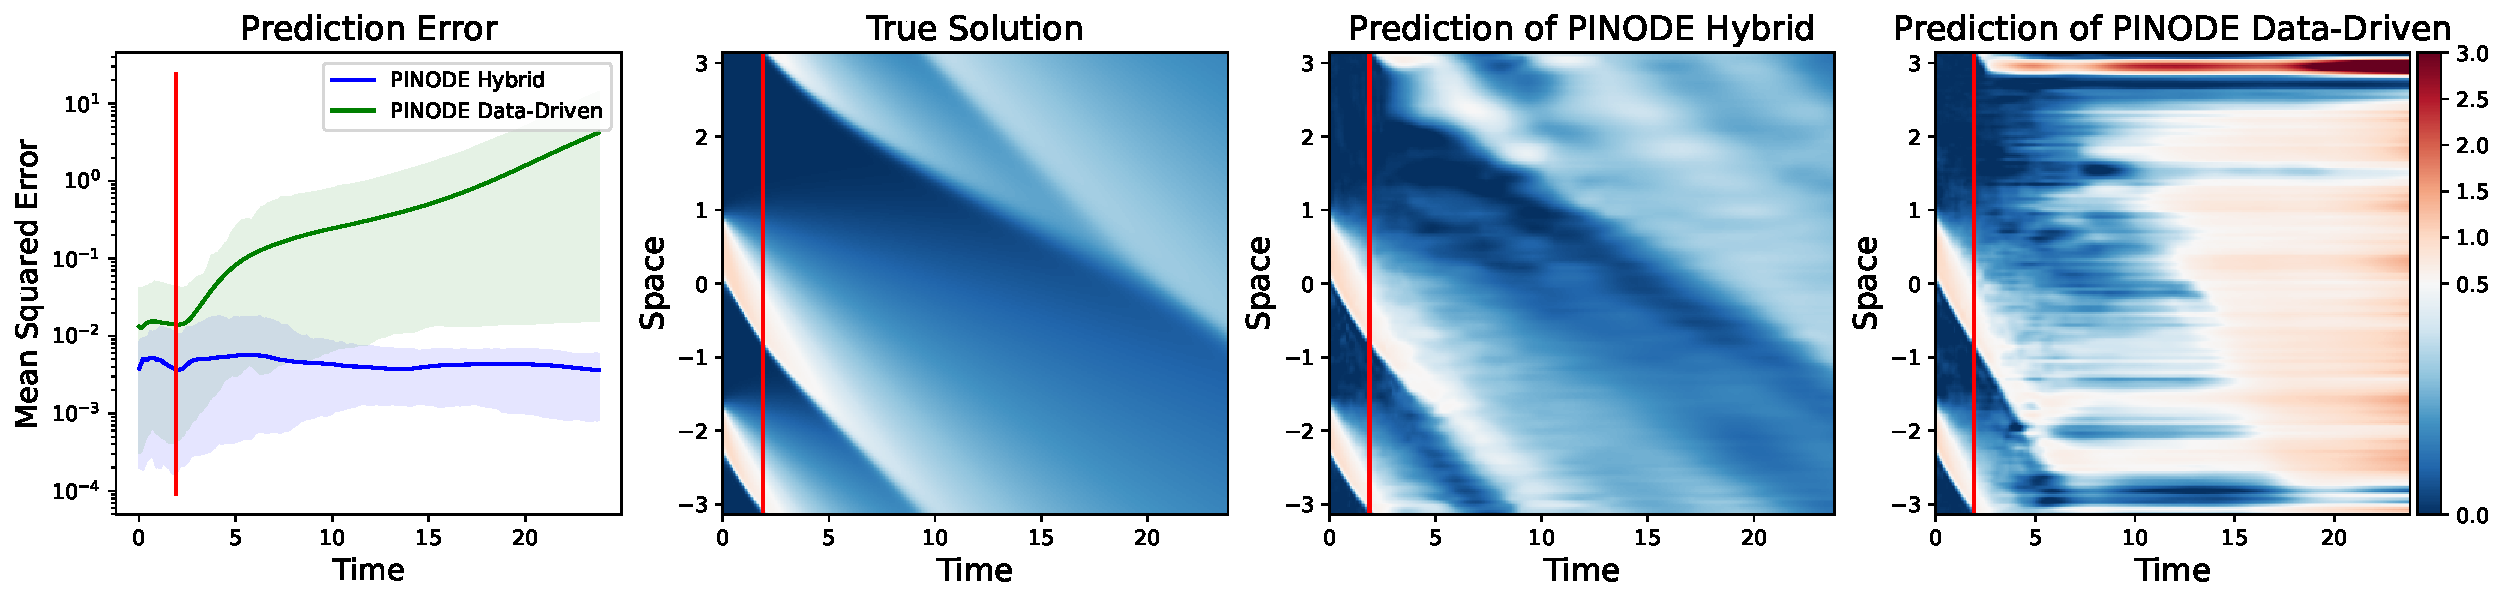
\includegraphics[width=0.9\textwidth]{figures/example_burgers.pdf}
    \caption{The first subplot shows the relative error of solving Burgers' equations on 100 test (unseen) initial conditions for two models: PINODE Hybrid and PINODE Data-Driven. Both models interpolate well but a purely data-driven model fails to extrapolate past the training time-horizon (left of the red vertical line). PINODE-Hybrid provides stable long-term predictions that points to its ability to correctly discover the low-dimensional manifold dynamics.}
    \label{fig:burgers_example}
\end{figure}

We also notice that the Hybrid models yield more stable and accurate predictions, relative to their purely data-driven counterparts, when forecasting far beyond the training time-period. In Figure~\ref{fig:burgers_example} we visualize the predictions for a test IC for two models: Data-Driven model from the bottom-left corner of Figure~(\ref{fig:burger_data_vs_collocations}), and a Hybrid model from the bottom-right corner of Figure~(\ref{fig:burger_data_vs_collocations}). The red line separates the time-period of training from the time-period of forecasting. The hybrid model's errors stay below $10^{-2}$ even when forecasting 10 times farther than what it was trained on. In contrast, the Data-Driven model shows low errors within its training time-region but the forecast errors grow quickly when forecasting beyond that.

\begin{figure}[ht]
    \centering
    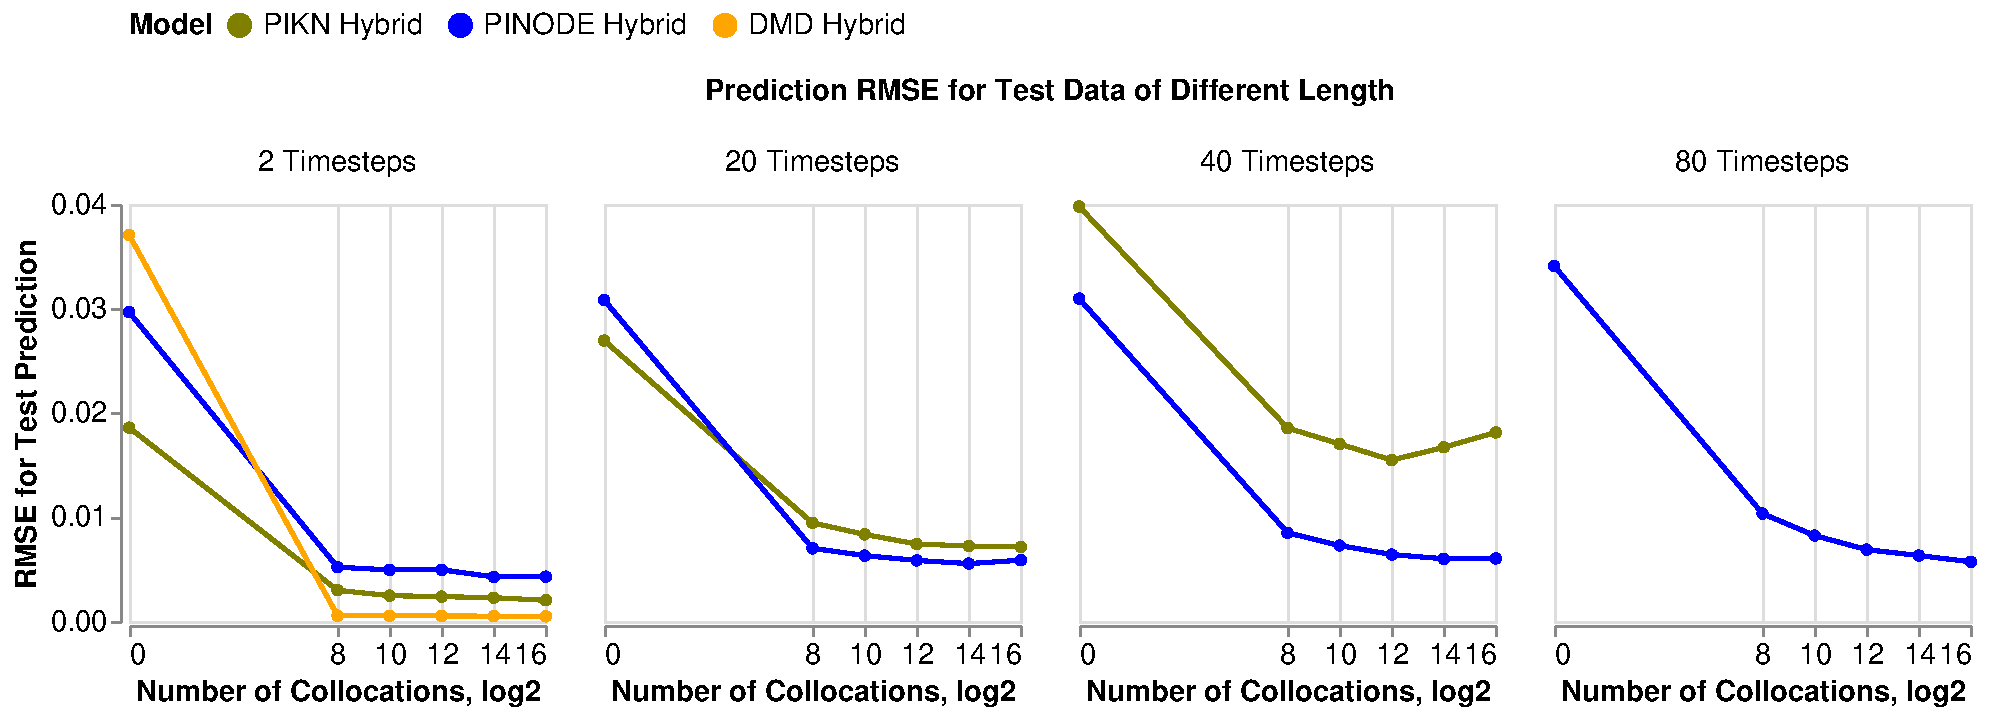
\includegraphics[width=0.9\textwidth]{figures/burgers_collocations_rmse.pdf}
    \caption{Collocation points improve results of all three models but they don't fix models' inherent shortcomings like instabilities in linear latent dynamics.\label{fig:burgers_collocations_rmse}}
\end{figure}

Finally, we observe that using collocation points can benefit other models, like DMD and PIKN. To illustrate, we replicate the experiments from Figure~\ref{fig:burger_data_vs_collocations} where the number of trajectories is 256 and with Bump ICs for PINODE, PIKN, and DMD.Figure~\ref{fig:burgers_collocations_rmse} shows the root mean squared error (RMSE) for the test data predictions as a function of the number of collocation points that were used in training.  The figure illustrates the prediction error for increasing prediction horizons going from left to right, and demonstrates that in all cases, PINODE benefits from the available collocation points. The leftmost panel shows that every model improves its one-step-ahead predictions, with DMD quickly achieving near-optimal performance. However, once the forecast horizon is increased to 20 timesteps ahead (length of the training trajectories) and above, DMD failed to correctly forecast the long-term trajectories and was removed from those figure to improve legibility. The PIKN models improved the one-step-ahead (1st pane) and interpolation performance (2nd pane) by a factor of 4. It also improved the extrapolation performance for 40-steps prediction (3rd pane) but failed to extrapolate for 80 steps (4th pane, removed for legibility). We attribute this behavior of PIKN to the possibility that the latent dynamics operator of PIKN contains positive eigenvalues despite the use of collocation points.

\subsection{Robustness to Noise in the Low-Data Regime}
\label{sec:burger_noise}
\begin{figure}[t]
    \centering
    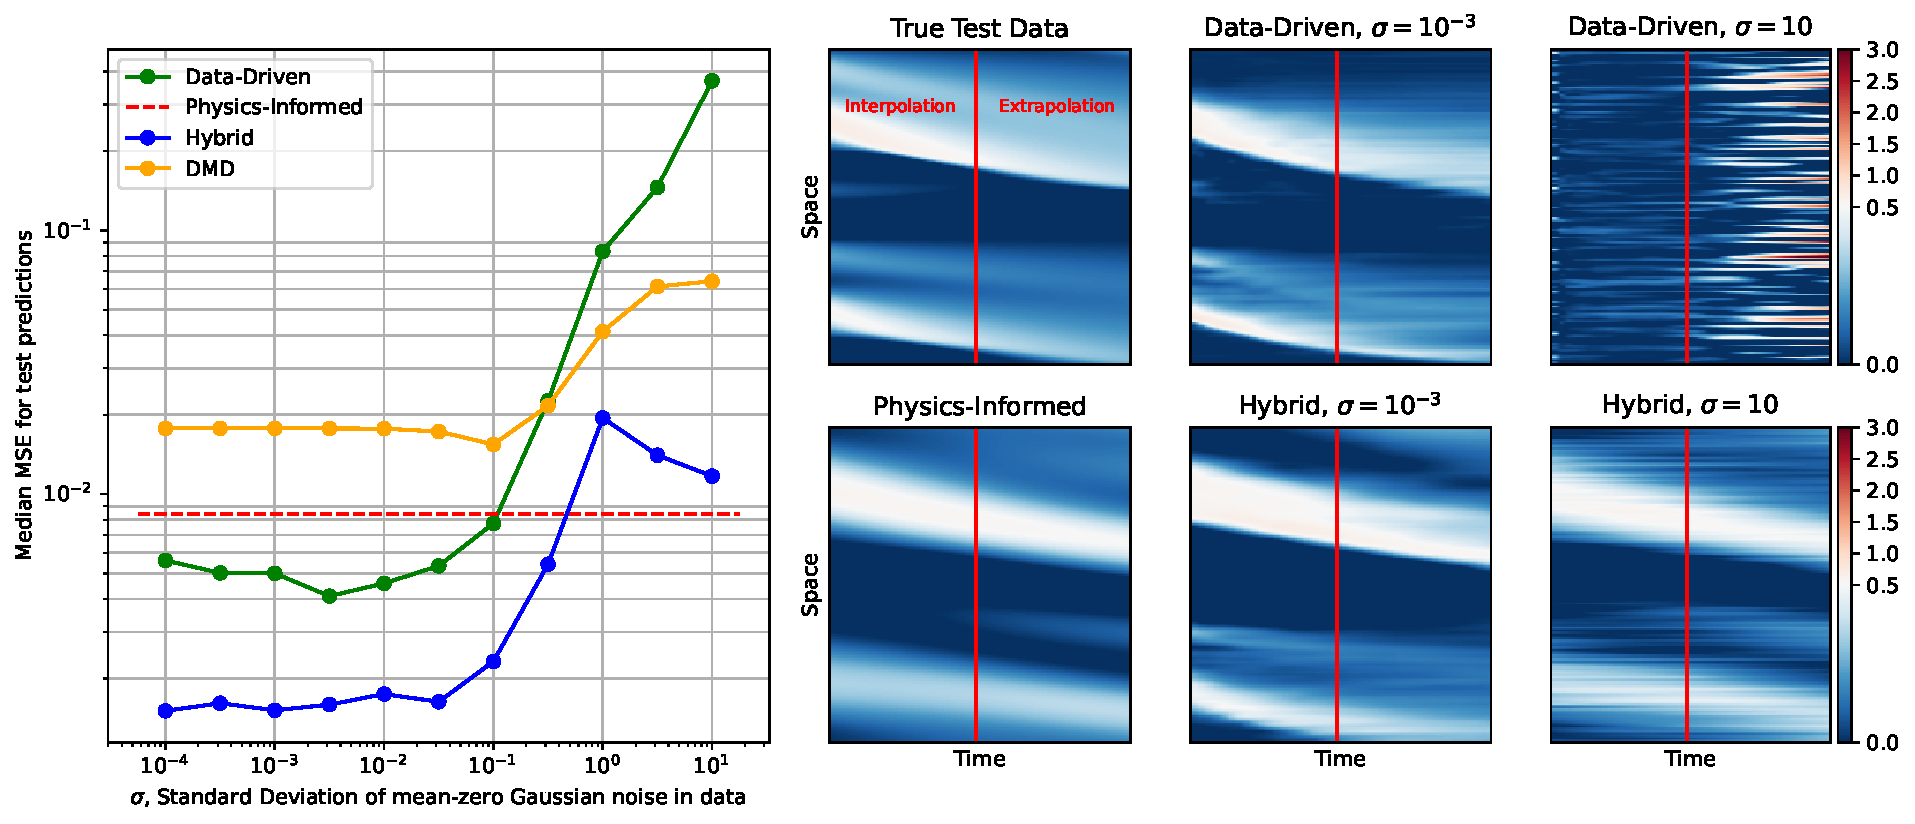
\includegraphics[width=0.9\textwidth]{figures/burgers_noise.pdf}
    \caption{Physics-informed loss works as a safeguard that prevents unbounded performance drop when quality of the data degrades due to noise. Namely, the solution of the hybrid loss~(\ref{eq:loss_combined}) converges to the solution of the physics-informed loss~(\ref{eq:loss_physics_informed}), when the data-driven loss~(\ref{eq:loss_physics_informed}) becomes uninformative. The performance of purely data-driven methods (Data-Driven, DMD) grows unbounded since these models don't have an alternative noise-independent source of information.}
    \label{fig:burger_noise}
\end{figure}

In this section we show that the use of collocation points improves the ROMs' robustness to noise in the data by providing an alternative, noise-free, source of information.

For this experiment, we use the Burgers' equation dataset containing 1024 trajectories with "bump" initial conditions, and 65536 "harmonic" collocation points as defined in Equation~\ref{eq:burger_collocations}. We then add i.i.d. Gaussian noise to the trajectories, with variance ranging from $\sigma = 10^{-4}$ to $\sigma = 10$. For reference, most of the data values lie between $0$ and $1$, so a noise level with $\sigma > 1$ dominates the data. We train four models: PINODE Hybrid, PINODE Data-Driven, PINODE Physics-Informed, and DMD. To measure the models' out-of-distribution prediction errors, we use the test dataset with Bump, Gaussian, and Harmonic initial conditions, as described in the previous subsection. The prediction errors are displayed in Figure~\ref{fig:burger_noise}, left pane. The prediction error of a purely Physics-Informed model (in red) is flat because the collocation points are noise-free. 

Figure~(\ref{fig:burger_noise}) shows that in the high noise setting, the error of purely data-driven models (DMD and PINODE Data-Driven) grows unbounded, whereas the performance of the hybrid model converges to the performance of the Physics-Informed model as the noise level increases. We hypothesise that such behavior is due to the second part~($\LL_{\theta}^{data}$) of the combined loss~(Eq.~\ref{eq:loss_combined}) turns into noise, and so its derivative also turns into noise.
\begin{equation}
    \nabla \LL_{\theta} = \underbrace{\nabla\LL_{\theta}^{physics}}_{\text{informative}} + \underbrace{\nabla\LL_{\theta}^{data}}_{\text{noise}}
\end{equation}
Thus, one can think about optimizing a hybrid model~(\ref{eq:loss_combined}) as about training a Physics-Informed model~(\ref{eq:loss_physics_informed}) using a noisy gradient descent with a fixed-variance noise. From the optimization literature \citep{friedlander2012hybrid,patel2021global,shapiro2021lectures} we know that, under certain conditions, such SGD converges to a neighbourhood of a local minimum of its loss (in this case $\LL_{\theta}^{physics}$) with high probability. So instead of diverging, a hybrid model turns into a Physics-Informed model; where the latter works as a performance safeguard in the high-noise regime.  On the right hand-side of Figure~(\ref{fig:burger_noise}), we show an example of the prediction performance of each of the models described above. The data-driven and hybrid models yield visually similar solutions when $\sigma = 10^-3$. However, the former provides inadequate performance when the data is dominated by noise, whereas a hybrid model in this regime produces a solution that is visually similar to the one that the Physics-Informed model produces. A more rigorous analysis of this phenomenon seems possible but lies outside of the scope of this work.


\section{Application to Compressive Sensing}
\label{ch:cs}
\subsection{Introduction}
% SPI definition and main stages
Single-pixel imaging (SPI) is a relatively recent imaging technique that replaces the classic two dimensional sensor array with a single photodetector~\cite{bian2018experimental}. An SPI camera modulates the incoming light from a scene using a light modulator, such as a diffuser~\cite{guo2016multilayer} or a digital micro-mirror device (DMD)~\cite{pittman1995optical, sampsell1993overview}, and focuses the resulting correlated light patterns onto a photodiode. The configuration of the modulator and the recorded intensity of light are then processed to reconstruct an image of the target scene.

% advantages of SPI
SPI owes its popularity to multiple advantages it achieves over traditional imaging approaches that employ 2D sensor arrays. First, since all reflected light is focused onto a single detector, SPI has better sensitivity under dim lighting conditions and enjoys a broader spectral range\cite{Edgar2019}. Second, SPI moves the cost of acquisition and processing from the encoding/compression stage to the decoding/reconstruction stage. For example, a DMD array orients its mirrors to reflect light either towards the detector (+1) or away from it (0). Importantly, these orientations do not depend on the scene that is being acquired to ensure proper reconstruction: \cite{baraniuk2008simple}~showed that DMD patterns can be drawn as independent identically distributed (i.i.d.) samples from a uniform Bernoulli distribution. In contrast, sample-then-compress approaches\cite{skodras2001jpeg} require an expensive projection of multiple single-pixel snapshots onto a chosen basis, such as Fourier or top-K singular vectors, during their encoding step. Doing the heavy-lifting job during decoding is often preferred in applications where sensors have to be small and low-power, whereas decoding happens offline on high-performance computers. The simplicity of encoding keeps the computational requirements of SPI sensors (and thus their price) low, inviting their application in multispectral imaging \cite{bian2016multispectral,li2017efficient}, optical encryption~\cite{chen2013ghost}, remote sensing~\cite{zhao2012ghost}, object tracking~\cite{li2014ghost}, and many other fields~\cite{sun20133d,zhang2010correlated,cheng2009ghost}.

% introducing CS
Compressive Sensing (CS)~\cite{donoho2006compressed, candes2006compressive, baraniuk2014introduction, baraniuk2008simple} emerged in the mid-2000s as an alternative signal acquisition regime to classical Shannon-Nyquist sampling. In the classical regime, a band-limited signal is sampled at $N$ specific points in time (and/or space) so that the signal can be reconstructed from the acquired samples using a simple Sinc interpolation. Compressive sensing, on the other hand, proposes to acquire the signal using a small number of inner products between the signal and general non-adaptive sampling vectors. If the signal to be acquired has a $K$-sparse, or more generally, parsimonious, representation some transform domain, then the signal can be guaranteed to be recovered using as few as $\mathcal{O}(K\log(N/K))$ non-adaptive measurements, which is much smaller than the $N$ samples that are required by sample-then-compress approaches such as JPEG and JPEG-2000~\cite{skodras2001jpeg}. The development of compressive sensing theory and efficient reconstruction algorithms has further promoted the deployment of this technique in SPI~\cite{duarte2008single}.

% Compressive Sensing (CS) is an approach to SPI which assumes that a signal is spare in a certain basis. Under this assumption a small collection of non-adaptive linear measurements can contain enough information for reconstructing the signal~\cite{duarte2008single, candes2006compressive}. Namely, when an original signal made of $N$ pixels has a $K$-sparse representation in a certain basis, the basis coefficients can be recovered using only $\mathcal{O}(K\log(N/K))$ which is much smaller than $N$ required by sample-then-compress approaches such as JPEG and JPEG-2000~\cite{skodras2001jpeg}.

% Recent progress on deep SPI
Because each CS measurement contains highly-compressed information about the observed frame, one needs to sample a large number of such measurements. Thus, many recent works propose approaches to reduce the number of required samples per frame (SPF). These approaches can be roughly grouped into two buckets: signal-dependent control of the mirrors and more sophisticated reconstruction techniques. The former ensures that each single-pixel measurement contains as much information as possible by focusing the mirrors on the selected regions of the frame~\cite{zhang2017fast,sun2017russian,xu20181000}. Although highly effective, such an approach cannot be applied to monitoring scenes that don't have a ``main zone'' where the information acquisition could be focused. For example, a camera monitoring a gas tank for leaks can not have a mask that works well for leaks appearing only in the middle of the scene. The second group of approaches focuses on creating more efficient optimization algorithms for the decoding step~\cite{katz2009compressive}. It includes non-iterative algorithms such as differential ghost imaging (DGI) \cite{gong2010method}, as well as iterative methods such as total variation (TV)~\cite{suo2016signal} regularization. Notably, recent approaches adopted deep learning (DL) for SPI reconstruction. These approaches showed that using deep neural networks can dramatically reduce sampling ratio and offer near-real-time performance \cite{lyu2017deep,higham2018deep,wang2019learning,wang2022single}. However, most of these methods use multiple samples for single-frame reconstruction and do not yield satisfactory reconstruction of multiple sequential frames when the number of samples per frame is small, even if the total number of samples is large, as we show below.

% Our place among CS literature
Our work aims to bridge this gap. It falls into the second group of decoding-centered approaches which aid CS reconstruction with deep learning. In particular, we show how a Reduced-Order Model (ROM) can be used to regularize CS reconstruction of a video of a physical phenomenon, even if all the measurements are taken at different moments in time. We achieve that by pre-training a ROM to compress simulations into a latent space and calculate the system's evolution there using neural ordinary differential equations (neural ODEs). At the time of reconstruction, we recover a trajectory in the latent space which yields compressing sensing measurements that match what the detector recorded when projected to the observable space. Effectively, we solve an ODE-regularized CS reconstruction in an efficient way using the adjoint-sensitivity method to obtain necessary derivatives~\cite{chen2018neuralode}. Such ODE-based regularization serves as a strong induced bias and reduces the number of samples per frame required for a successful reconstruction. In fact, our method requires fewer samples per frame than the current state-of-the-art methods. We introduce the methodology in Section~\ref{sec:cs_methods} and study its performance on two examples: Burger's equation and Kolmogorov flow.

\subsection{Methods}
\label{sec:cs_methods}
\begin{figure}
    \centering
    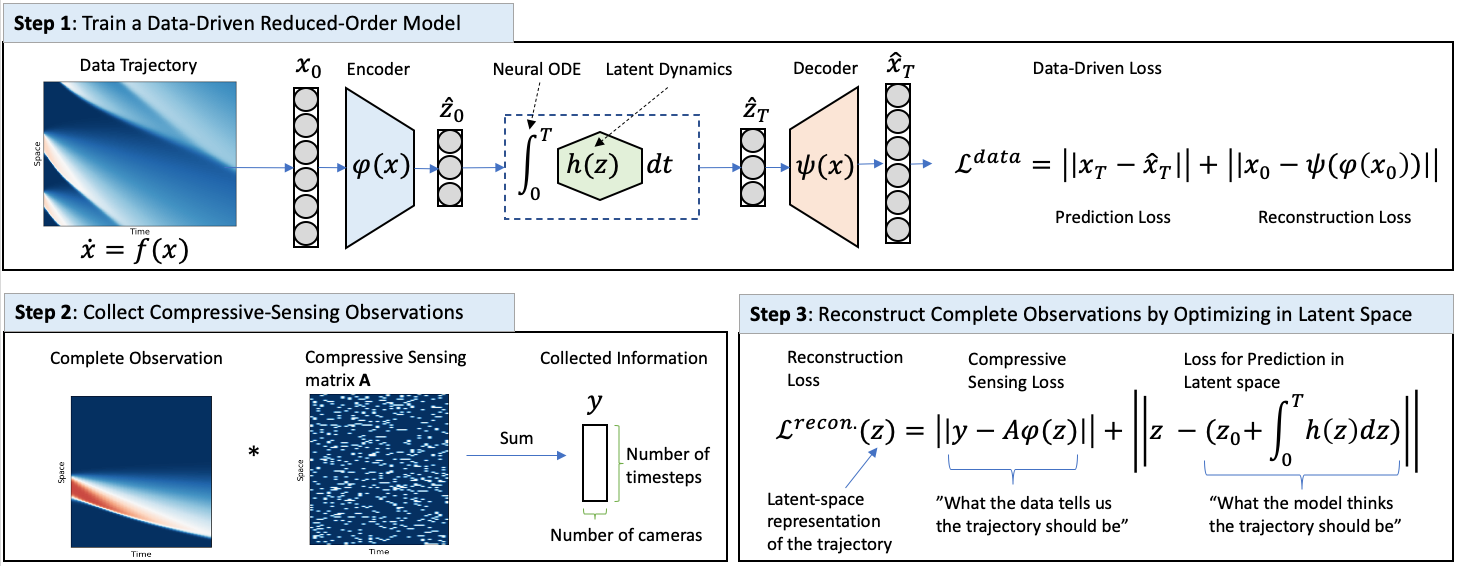
\includegraphics[width=\textwidth]{figures/cs_abstract.png}
    \caption{\label{fig:cs_abstract}We propose a compressive-sensing algorithm that reconstructs observations by identifying their trajectories in a latent space of a Reduced-Order Model (ROM). The model provides strong inductive bias and reduces data intake requirements for compressive-sensing hardware.}
\end{figure}

\paragraph{Reduced-Order Model with Non-Linear Latent Dynamics} We assume the same notation as in Section~\ref{sec:method} and define a reduced-order model (ROM) as a tuple $(\psi_\theta, \phi_\theta, h_\theta)$, which consists of a decoder $\psi_\theta(z)$, an encoder $\phi_\theta(z)$, and the latent dynamics $h(z)$, respectively, all parametrized by trainable weights $\theta$. We also assume that it is technically possible\footnote{For example, if $h(z)$ is a neural network, then one can evaluate such an integral using adjoint-sensitivity-based techniques, e.g. \texttt{torchdiffeq} package by \cite{chen2018neuralode}.} to evaluate a differentiable integral over the latent dynamics $h(z)$ for a given period of time. Figure~\ref{fig:cs_abstract} illustrates the architecture of the ROM. We assume that such ROM comes fully trained, so we consider its weights $\theta$ to be frozen and omit them from the notation. 

\paragraph{Compressive Sensing} In many applications, we can not observe $x(t)$ in real time. Instead, as illustrated on Figure~\ref{fig:cs_abstract} (Step 2), we observe $p$ scalar values per timeframe, with each scalar a linear combination of a small number of coordinates of $x(t)$ at a time:

\begin{equation}
    \label{eq:cs_definition}
    \tilde{y}(t) = A_t x(t), \quad A_t \in \mathbb{R}^{p\times n}
\end{equation}

When recorded over a discretized period of time $[t_1, \dots, t_T]$, such a set of observations is stored as a vector, $y \in \mathcal{R}^{T \times p} = [y(t_1), \dots, y(t_T)]^T$.

\begin{figure}
\centering
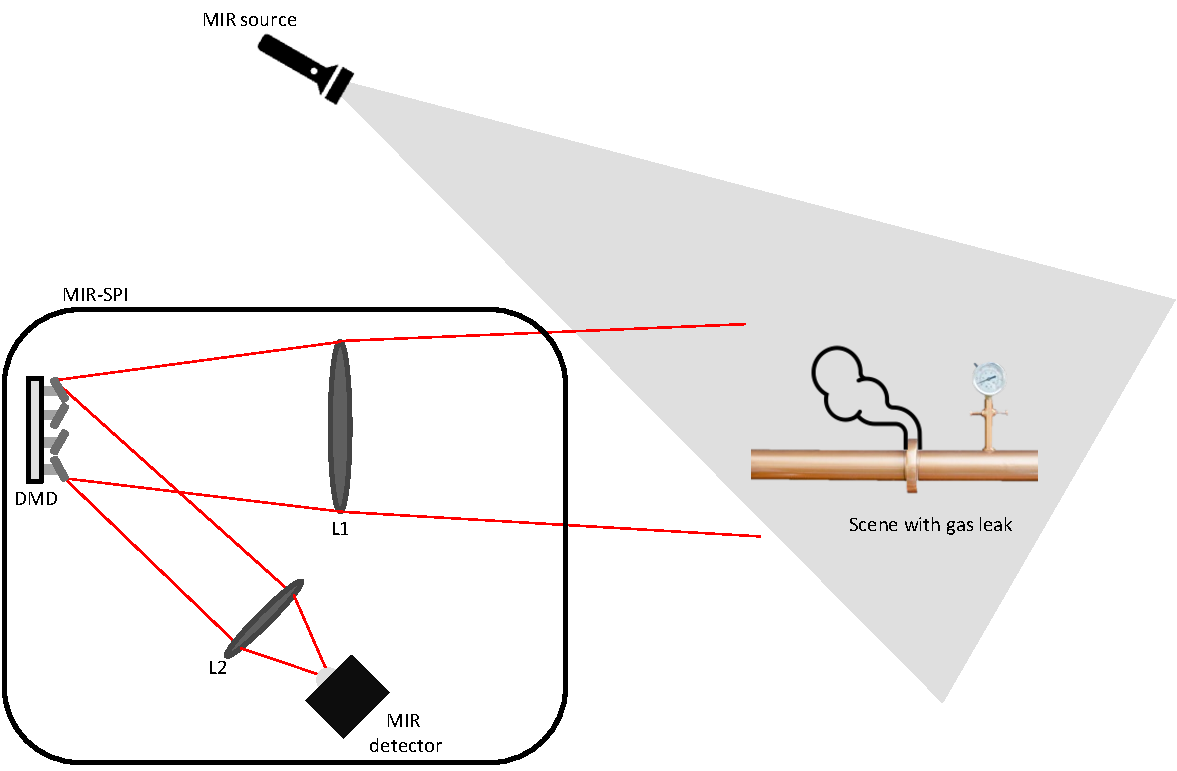
\includegraphics[width = 0.5\textwidth]{figures/SPI_setup.pdf}
\caption{SPI setup with DMD \label{fig:SPI}}
\end{figure}

We consider a single pixel camera setup in which, for every time instance $t$, $p$ acquisitions $y(t)$ are obtained by a high sampling rate photo-detector using the projection matrix $A_t$. The rows of the matrix $A_t$ correspond to a binary mask pattern that can be encoded using a digital micro-mirror device (DMD, \cite{pittman1995optical, sampsell1993overview}). Similarly to the setup from~\cite{duarte2008single}, the mirrors of our (idealized) DMD array represent pixels of the future reconstructed image, and the slopes of the mirrors represent the weights. The light from a scene lands on a DMD, which slopes each of its mirrors to reflect light either towards the detector (+1) or away from it (-1) according to a uniform Bernoulli variable. Next, the (+1) pixels go through a double-convex lens that focuses them on a signal photon detector. Finally, the detector integrates the signal and provides the final observation as its output voltage, which is later digitized by an A/D converter. The slopes of each mirror are also recorded in the detector's memory. Figure~\ref{fig:SPI} illustrates an example of the single pixel imaging setup where a gas plume is imaged using a DMD array and a medium infrared (MIR) photo-detector. 

A modern DMD supports snapshot frequencies of around 10~kHz (\cite{wang2022single}). When the scene changes much slower one can assume that such a device can take multiple measurements of a scene simultaneously\footnote{When the dynamics change rapidly, one would have to use an array of DMD devices to achieve more than one sample per frame}. The number of samples recorded per  frame is referred to as \textit{samples per frame}, or SPF. It is often divided by the total number of mirrors of the DMD device and multiplied by 100\%, in which case it is called a \textit{sample per frame rate} $\beta$. For a compressive-sensing-based image reconstruction approach to be practically useful it should require a relatively small rate $\beta$ (e.g. 2-10\%) for a successful reconstruction  of the scene.

\paragraph{Reconstruction Loss} It is often possible to have access to the complete state $x(t)$ at the moment of model training. Thus, one can develop a ROM $(\psi_\theta, \phi_\theta, h_\theta)$ using the full state $x(t)$, and then utilize this ROM for real-time compressive sensing applications. In particular, we use the ROM $(\psi_{\theta^*}, \phi_{\theta^*}, h_{\theta^*})$ from Figure~\ref{fig:cs_abstract}~(Frame 1) to forecast the dynamics based on partial observations in real time. Namely, instead of reconstructing $x(t)$ based on compressive-sensing observations $y(t)$ directly, we first reconstruct the latent dynamics $z(t)$ and then project it to the observable space using the decoder $\psi_{\theta^*}(z)$, as illustrated in Figure~\ref{fig:cs_abstract}, bottom-right pane. 

\begin{align}
    \label{eq:reconstruction_problem_differential}
    \min_{\{z_t\}_{t=1, \dots, T}} & \frac{1}{2}\sum_{t=1}^T \left\|y_t - A\psi_{\theta^*}(z_t)\right\|_2^2 \\
    \text{s.t. } & \dot{z} = h_{\theta^*}(z)
\end{align}

We integrate the constraint and write it in its Lagrangian form:
\begin{align}
\label{eq:reconstruction_problem_integral}
    \min_{\{z_t\}_{t=1, \dots, T}} \LL_{\theta^*}^{recon}(z)
\end{align}

where 

\begin{equation}
    \label{eq:reconstruction_loss}
     \LL_{\theta^*}^{recon}(z) = \frac{1}{2}\sum_{t=1}^T \left\|y_t - A\psi_{\theta^*}(z_t)\right\|_2^2 + \frac{\lambda}{2} \sum_{t=1}^T \left\|z_{t-1} + \int_{t-1}^{t}h_{\theta^*}(z)dz - z_t\right\|_2^2
\end{equation}

where the parameter $\lambda$ controls the degree on which the compressing sensing algorithm relies on the latent dynamics $h_{\theta^*}$ during the signal reconstruction phase. We minimize the loss~\eqref{eq:reconstruction_loss} using a gradient-based technique, with the gradients obtained using automatic differentiation frameworks. 

\subsection{Experiments}

\subsubsection{Burger's Equation}
We study the performance of our framework on Burger's equation with $[-\pi, \pi]$-periodic boundary conditions:

\begin{equation}
\begin{split}
    & u_t  + uu_x = \nu u_{xx} \\
    & u(-\pi, t) = u(\pi, t),\quad \forall t \in [0, T]
\end{split}
\end{equation}
where $u_t$, $u_x$, and $u_{xx}$ denote the first partial derivative in time, and the first and second spatial derivatives, respectively.

\paragraph{ROM Training} To obtain training data for the ROM, we replicate the experimental setup from Section~\ref{sec:compressibility}. Namely, we generate 1024 trajectories on a discretized spacial domain $[-\pi,\,\pi]$ with 128 grid points. To generate a diverse set of initial conditions, we sum the first 10 harmonic terms with random coefficients:
\begin{equation}
    \label{eq:burger_initial_condition_sine}
    u(x, 0) = \frac{1}{10}\sum_{k = 1}^{10} a_k\cos(kx) + b_k\sin((k+1)x), \quad a_k, b_k \sim \mathcal{N}(0, 1)
\end{equation}
 We solve Equation~\ref{eq:burgers_equation} for $t \in [0, 2]$ with $\Delta t = 0.1$ using a spectral solver by~\cite{trefethen2000spectral}. 

\paragraph{Compressive Sensing}
For the compressive sensing phase, we generate 128 trajectories with ``bump'' initial conditions -- a smooth approximation of a bump with two opposing steeply-curved sigmoids:

\begin{equation}
    \label{eq:burger_initial_condition_bumps}
    u(x, 0) = \frac{1}{1 + exp(-k(x-a))} - \frac{1}{1 + exp(-k(x-b))}
\end{equation}

where $a < b$ are sampled uniformly in $[-\pi, \pi]$ and $k = 20$. We choose this shape to ensure that the training and sensing trajectories are sufficiently different. We choose compressive sensing matrices $A_t$ to be binary (0-1) matrices with each row having 64 non-zero components out of 128 sampled uniformly.

We compare our approach (PINODE) with four alternatives: Digital Ghost Imaging (DGI) by~\cite{ferri2010differential} and~\cite{gong2010method}, its Autoencoder-enhanced variation (DGI+Conv. Decoder) by~\cite{wang2022single}, Total Variation Regularization  (TVR) by~\cite{bian2018experimental}, and an approach by~\cite{bora2017compressed} which uses an autoencoder (AE). We measure reconstruction accuracy with three commonly-used metrics: the residual mean-squared error (RMSE), the peak signal-to-noise ratio (PSNR), and the structural similarity index measure (SSIM). We evaluate both metrics for Burger's trajectories as 2D-images in spatial and in temporal domains. 

For two 2D images $a$ and $b$, PSNR is defined as the log-ratio of the maximal value from the true image:

\[
	\text{PSNR}(a, b) = 20\log\left(\frac{\max_{i,j}(|a[i,j]|)}{\|a - b\|_2}\right)
\]

SSIM is defined as a product of relative luminance $l(a,b)$, contrast $c(a,b)$, and structure $s(x,y)$:

\[
	\text{SSIM}(a, b) = l(a,b) \cdot c(a,b) \cdot s(a,b) = \left(\frac{2\mu_a\mu_b + c_1}{\mu_a^2 + \mu_b^2 + c_1}\right) \cdot \left(\frac{2\sigma_a\sigma_b + c_2}{\sigma_a^2 + \sigma_b^2 + c_2} \right) \cdot \left(\frac{\sigma_{ab} + c_2/2}{\sigma_a \sigma_b + c_2/2}\right)
\]
Finally, RMSE is defined as the mean residual squares for every state, averaged over the temporal axis:

\[
	\text{RMSE}(a,b) = \|a - b\|_F
\] 

where, for a picture $x$, $\mu_x$ is the pixel sample mean, $\sigma_x$ is the standard deviation,  and $c_i$ are the constants which stabilize the division when the denominator approaches 0. Typically, $c_i$ are set to be proportional to the square of the dynamic range of the pixel values, e.g.  $c_i = (k_i*2^{\text{bits per pixel}} - 1)^2$, with $k_1 = 0.01$ and $k_2 = 0.03$ being default choices.


\begin{figure}
    \centering
    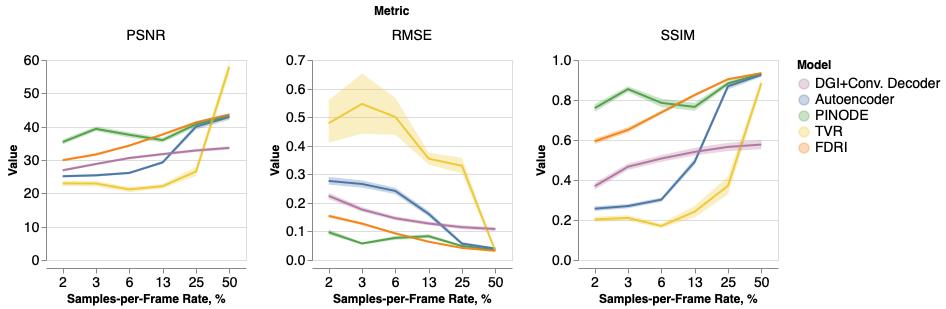
\includegraphics[width=\textwidth]{figures/cs_burgers_psnr.png}
    \caption{\label{fig:cs_burgers_spf} Median PSNR, RMSE, and SSIM with 25-27th percentile intervals over different number of samples per frame taken. We see that PINODE achieves 70\% higher peak signal-to-noise-ratio (PSNR), and 4 times higher structural similarity index measure (SSIM) when SPF is low, than its nearest competitor (AE).}
    
\end{figure}

\begin{figure}
    \centering
    	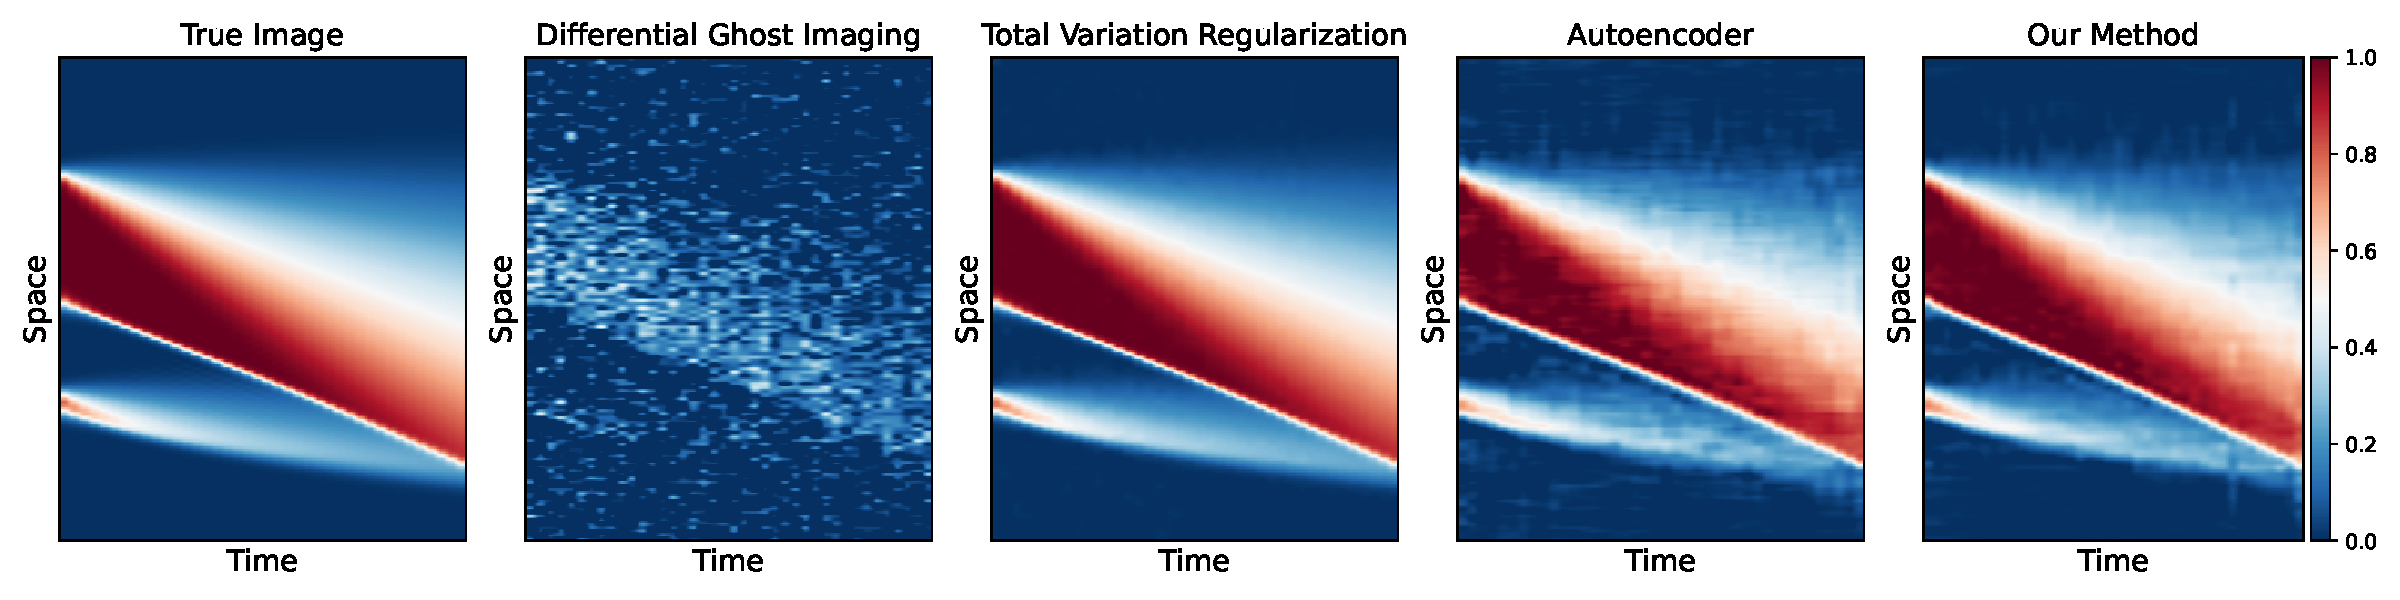
\includegraphics[width=\textwidth]{figures/cs_burgers_comparison_64.pdf}
    \caption{\label{fig:cs_burgers_example_large_spf} Example reconstruction with 32 samples per frame (SPF), an SPF rate of 50\%. Rather unsurprisingly, all algorithms complete the reconstruction faithfully due to a large amount of samples.}
\end{figure}

\begin{figure}
    \centering
    	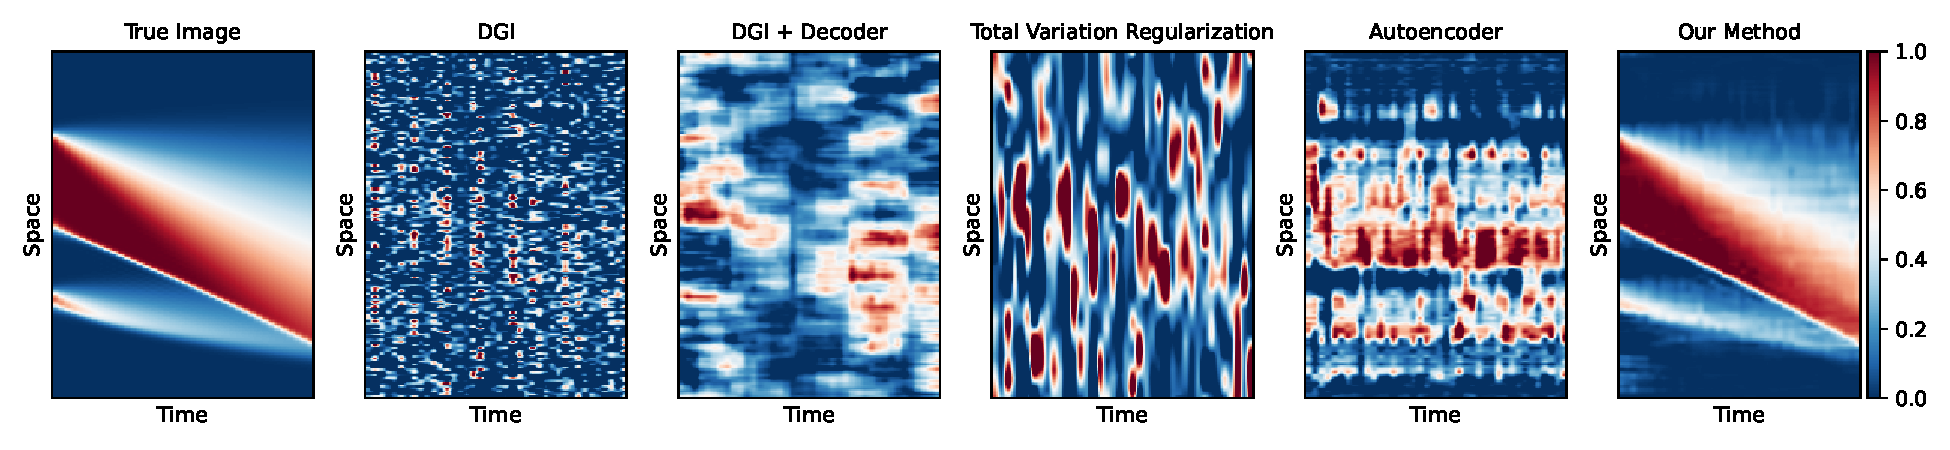
\includegraphics[width=\textwidth]{figures/cs_burgers_comparison_4.pdf}
    \caption{\label{fig:cs_burgers_example_small_spf}Example reconstruction with 2 samples per frame (SPF). All algorithms except our proposed method fail to recover the image due to the insufficient SPF rate (~3\%). In contrast, our proposed method achieves nearly the same reconstruction quality as in Figure~\ref{fig:cs_burgers_example_large_spf} with SPF rate of 50\%.}
\end{figure}

\paragraph{Results} The results are presented in Figure~\ref{fig:cs_burgers_spf}. We plot median PSNR, RMSE, and SSIM over different number of samples per frame taken. We see that PINODE achieves 70\% higher peak signal-to-noise-ratio (PSNR) and 4 times higher structural similarity index measure (SSIM)  relative other algorithms when SPF is low. We also see that the DGI and TVR approaches do not reconstruct images faithfully until SPF approaches the number of pixels in a snapshot; Figure~\ref{fig:cs_burgers_example_large_spf} provides an example of high-SPF reconstruction. In contrast, PINODE is able to reconstruct most trajectories with high accuracy using a very small number of samples per frame e.g. two samples, as visualized on Figure~\ref{fig:cs_burgers_example_small_spf}. It happens because the reduced-order model of PINODE serves as a strong prior: the model reconstructs the trajectory as a whole instead of reconstructing every snapshot separately, as all other algorithms do in this comparison. It allows PINODE to borrow strength across snapshots, even when SPF per each snapshot is small.

We also study robustness of PINODE approach to noise in compressive samples $y$ relatively to other algorithms. Figure~\ref{fig:cs_burgers_noise_aggregate} presents an aggregated comparison of reconstruction of solutions of Burger's equations under noise for SPF=12.5\%; the setup is equivalent to the one for SPF = 8 on Figure~\ref{fig:cs_burgers_spf} . Namely, we plot performance metrics (PSNR, RMSE, SSIM) of reconstructions from different models against Signal-to-Noise Ratio (SNR) in the vector of compressive sensing single-pixel observations $y$. The performance of PINODE remains superior until all models start reconstructing the scene very poorly. Figure~\ref{fig:cs_burgers_noise_examples} visualizes reconstructions for selected levels of SNR. We see that PINODE is able to provide a faithful reconstruction even under a substantial noise (e.g. third column).

\begin{figure}
	\centering
	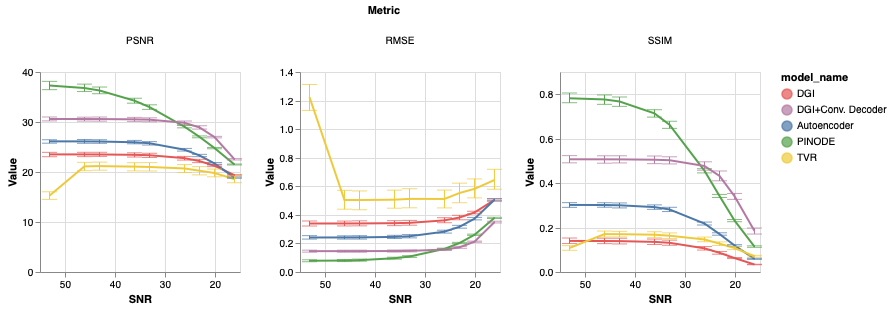
\includegraphics[width=\textwidth]{figures/cs_burgers_noise_aggregate.png}
	\caption{\label{fig:cs_burgers_noise_aggregate} Performance of reconstruction of solutions of Burger's equations under noise for SPF=12.5\%. We plot the performance metrics of different models against Signal-to-Noise Ratio (SNR) in the vector of compressive sensing single-pixel observations $y$. The performance of PINODE remains superior until all models start reconstructing the scene very poorly. See Figure~\ref{fig:cs_burgers_noise_examples} for example visualizations.}
\end{figure}

\begin{figure}
	\centering
	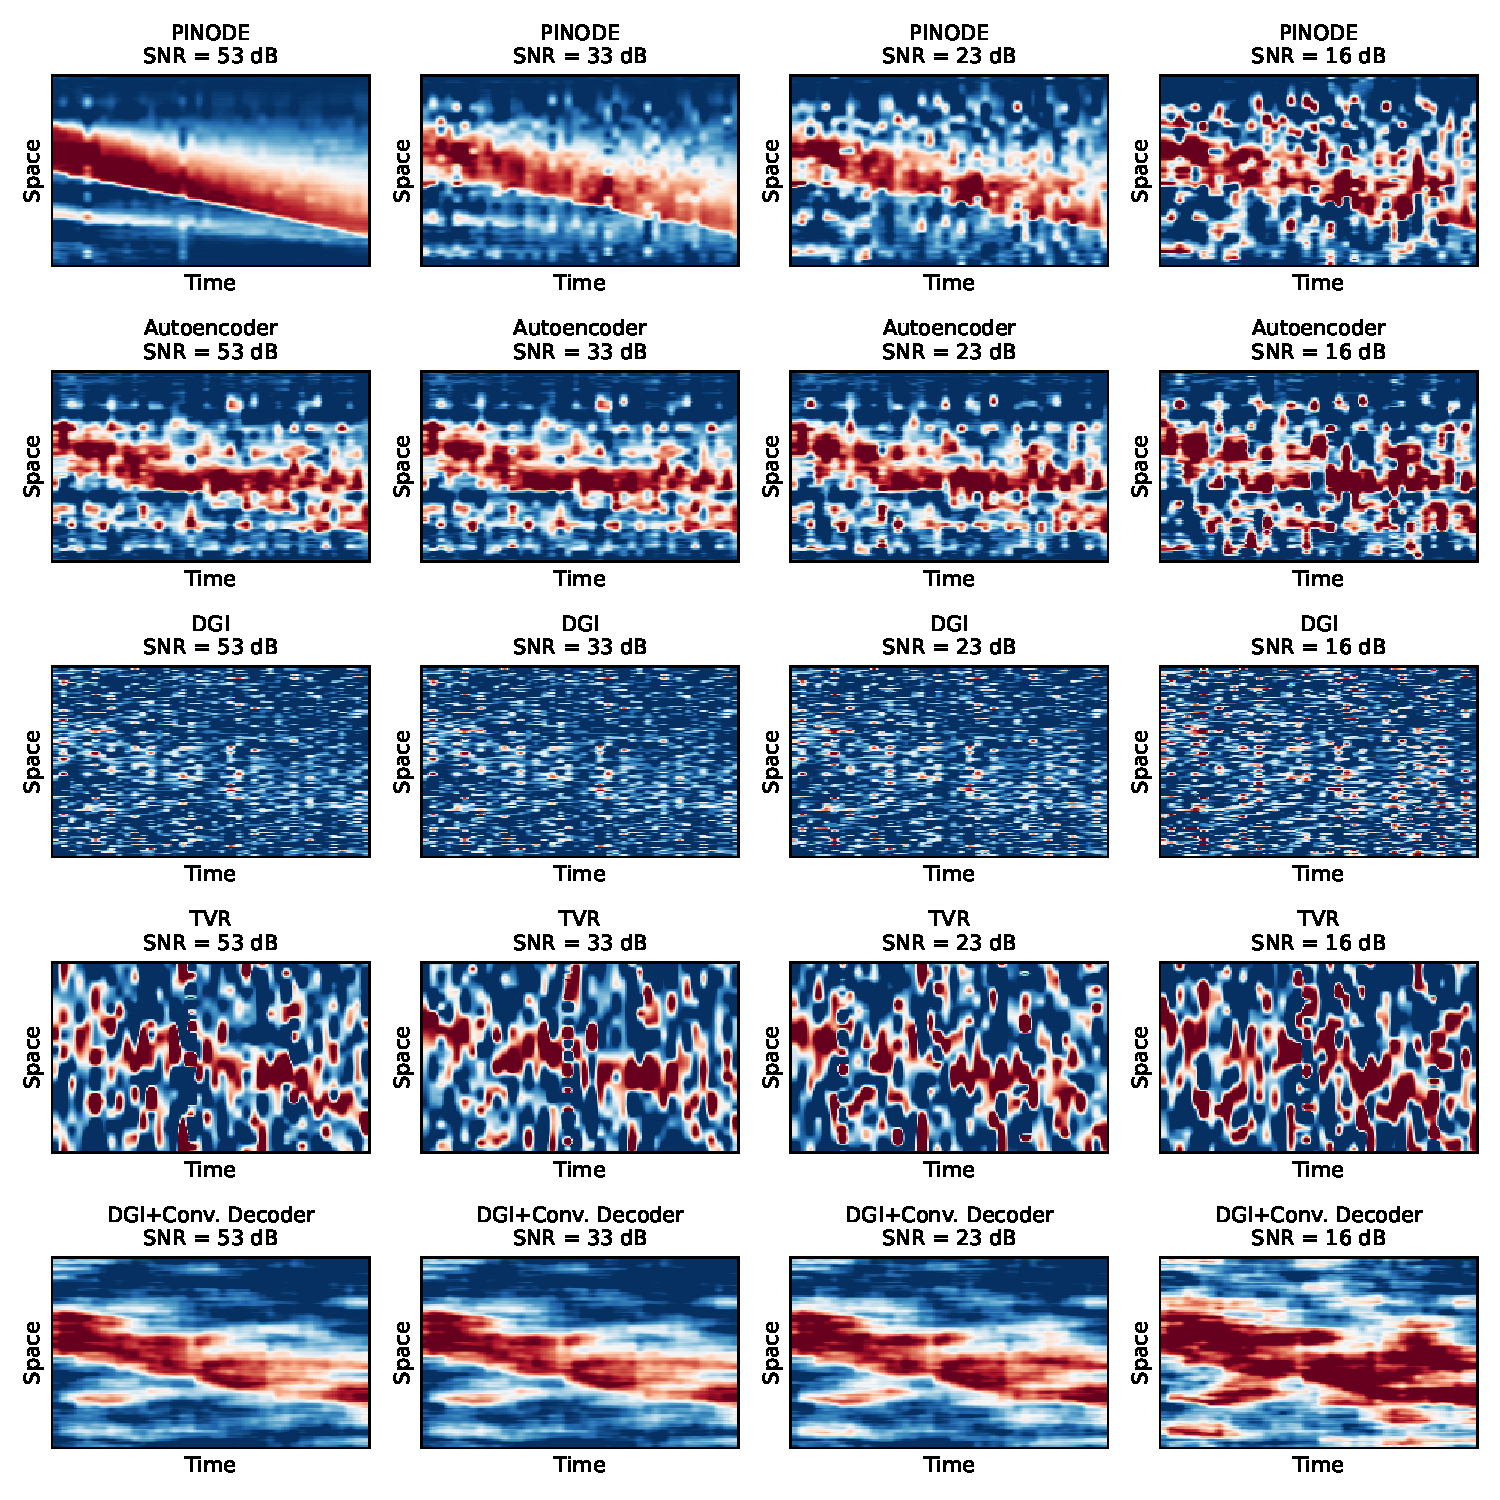
\includegraphics[width=\textwidth]{figures/cs_burgers_noise_examples.pdf}
	\caption{\label{fig:cs_burgers_noise_examples} Examples of compressive-sensing reconstructions of trajectories of Burger's equation under noise from Figure~\ref{fig:cs_burgers_noise_aggregate}.}
\end{figure}

 


\subsubsection{Kolmogorov Flow}
\label{sec:kolmogorov_flow}
We study the performance of our framework on Kolmogorov-like flow first-described by~\cite{dovzhenko1981generation} and later analyzed by \cite{tithof2017bifurcations,suri2017forecasting}. The following equation describes the behavior of a 2D velocity field $\bd{u}(x, y, t)$:


\begin{align}
\label{eq:kolmogorov_flow_definition}
	& \partial_t \bd{u} + \bd{u} \cdot \nabla \bd{u} = -\nabla p + \nu\nabla^2\bd{u} + f \\
	& \nabla \cdot \bd{u} = 0
\end{align}

where $p$ is a 2D pressure field, $f = \alpha\sin(ky)x$ represents the driving force with amplitude $A$ and wavenumber $k$, and $\nu = 1/\text{Re}$ is the non-dimensional viscosity equal to inverse of the Reynolds number. In all our experiments, $k = 4$ and $\text{Re} = 40$; we chose this setup to match the one from~\cite{wan2018data}, who identified that this combination of hyper-parameters leads to the occurrence of extreme instability events, making the prediction of such flow truly challenging. 

To train a ROM which predicts $u(x, y, t)$ we generate 8192 data trajectories as solutions of~\eqref{eq:kolmogorov_flow_definition} using a spectral solver\footnote{\href{https://github.com/zhong1wan/data-assisted/blob/master/Kolmogorov/kol2d_odd.py}{https://github.com/zhong1wan/data-assisted/blob/master/Kolmogorov/kol2d\_odd.py}} from~\cite{wan2018data}. Each solution was simulated from t=0 to t=100 to get past the transient regime and then recorded from t=100 to t=110, with the time-step $dt=0.5$. As in Section~\ref{sec:method}, the ROM consists of an encoder $\phi(u)$, a decoder $\psi(z)$, and the latent dynamics $h(z)$. It was trained by minimizing the data-driven loss~\eqref{eq:loss_data_driven} until the prediction RMSE on a holdout set stopped improving, which took about 60 epochs. 

\begin{figure}
	\centering
	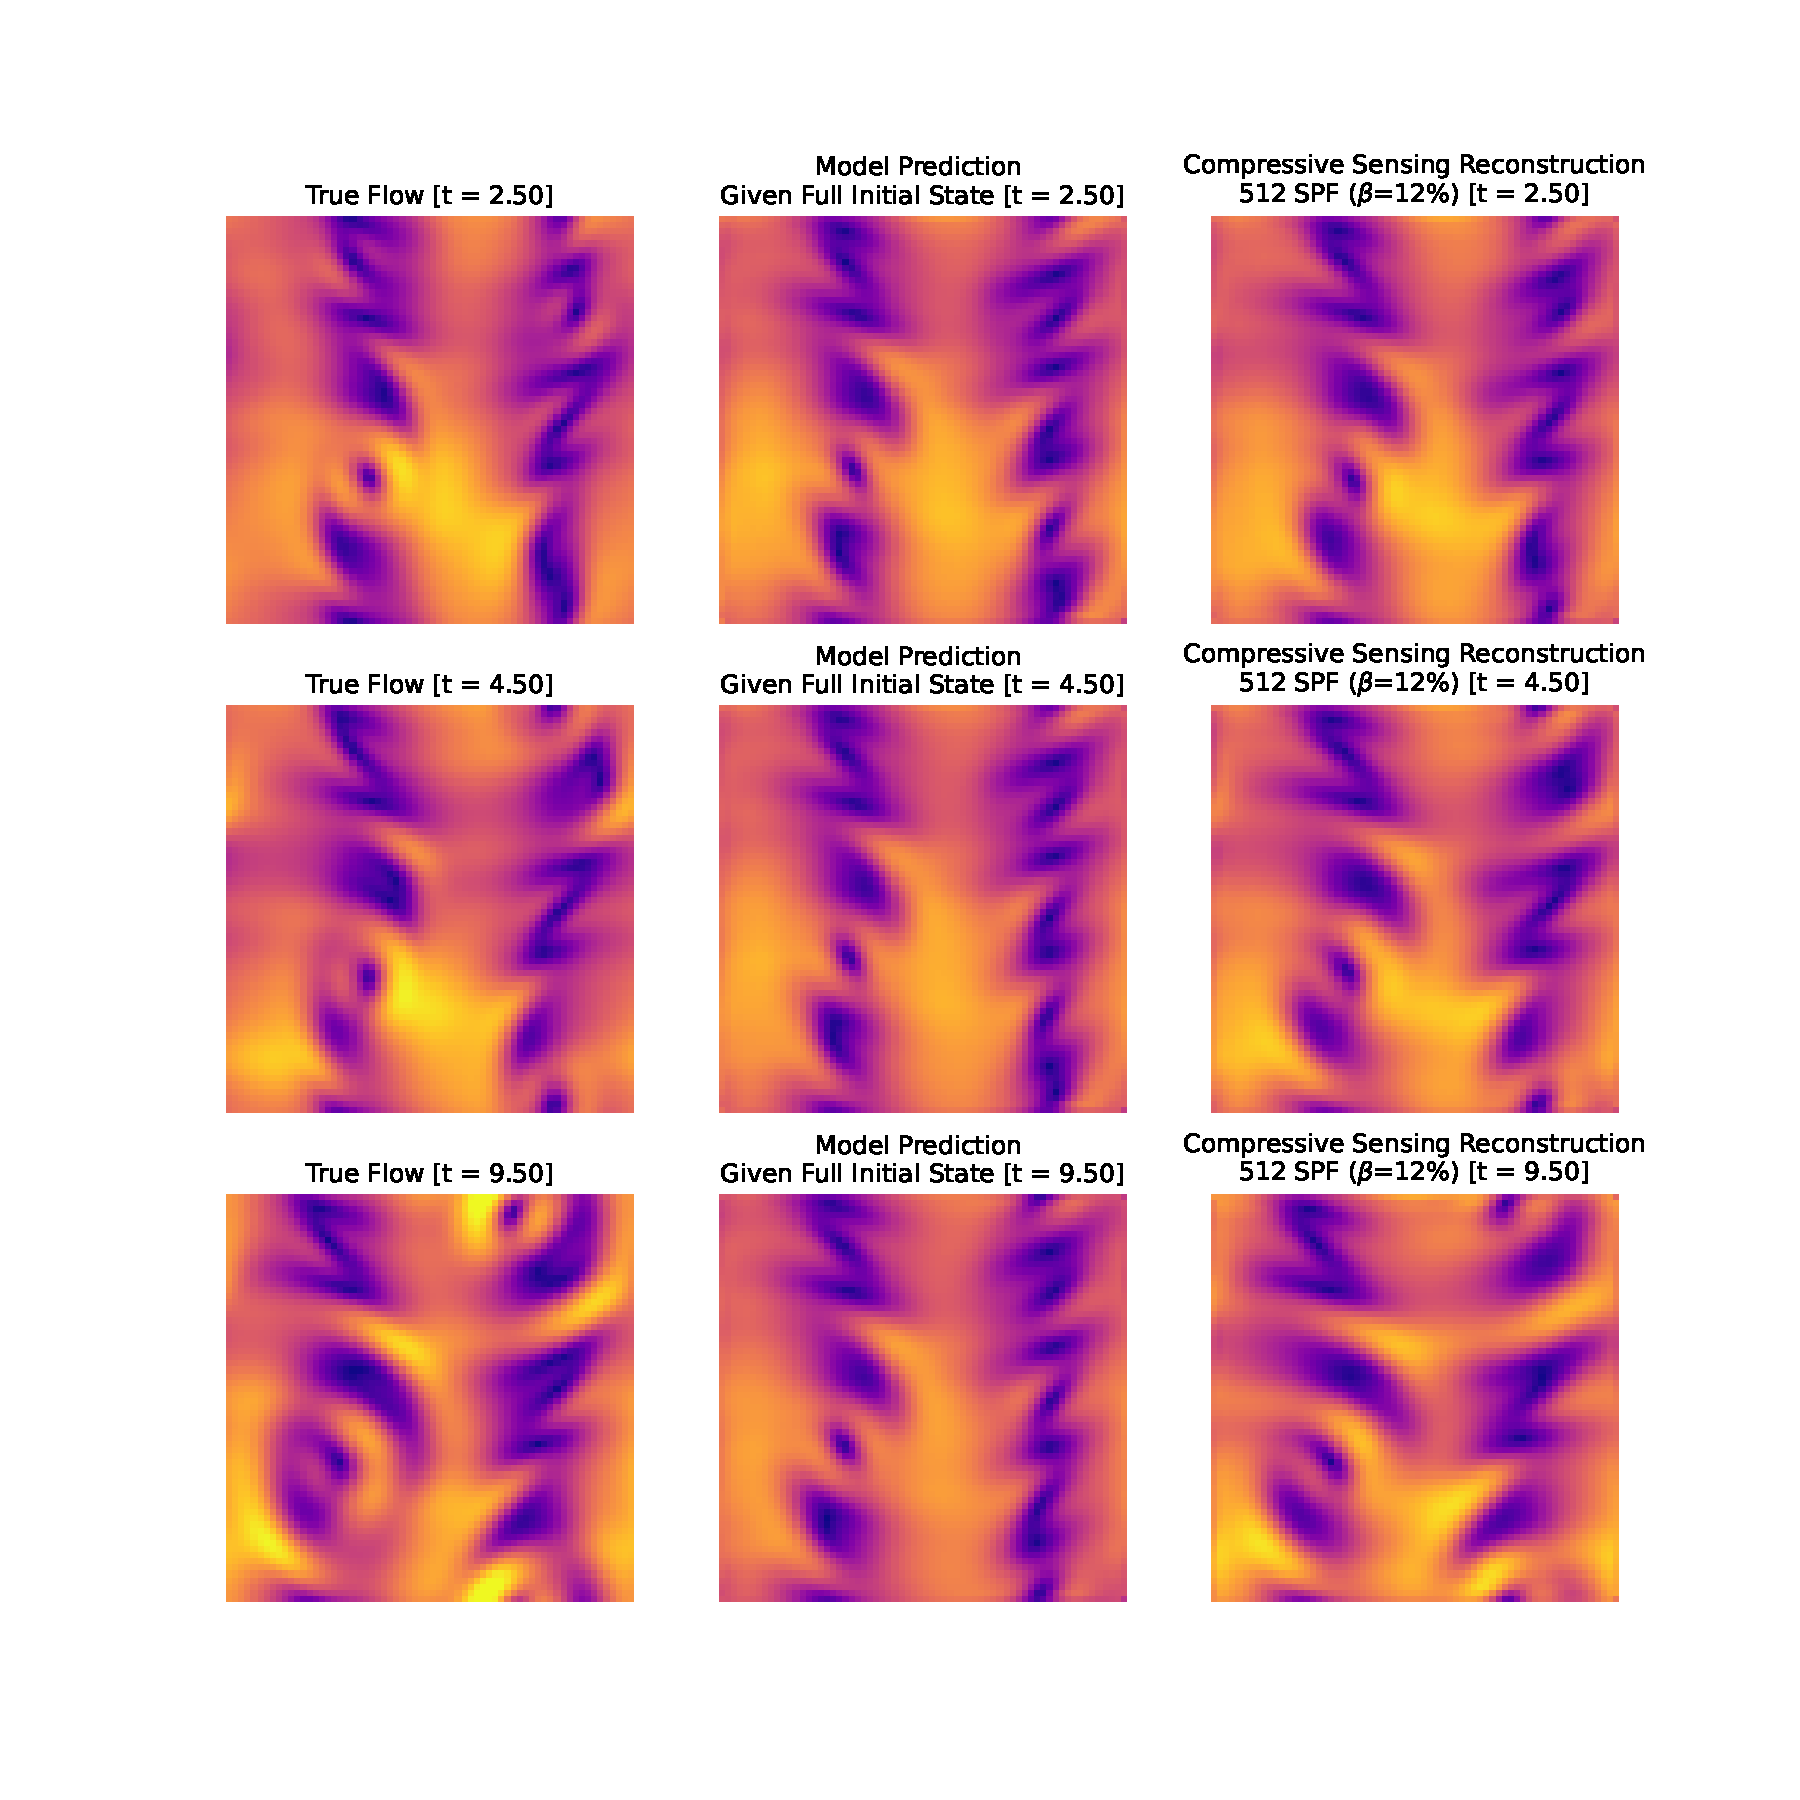
\includegraphics[width=\textwidth]{figures/kolmogorov_example.pdf}
	\caption{\label{fig:kolmogorov_example} An example of a compressive-sensing reconstruction of Kolmogorov flow using a ROM-regularized method. The rows represent three different moments in time. The first column represents the true flow. The second column represents a prediction of the ROM if the initial state of the system were to be known. The third column displays the results of CS reconstruction of our algorithm with 512 samples per frame.}
\end{figure}

A sample result is displayed on Figure~\ref{fig:kolmogorov_example}. The rows represent three different moments in time. The first column represents the true flow. The second column represents the prediction of the ROM if the initial state of the system were to be known to the model. It is unknown, so the second row serves as a reference performance of an underlying ROM. The third column displays the results of CS reconstruction of our algorithm with 512 samples per frame. Each frame is $66\times 66=4356$ pixels, which yields a sampling-per-frame rate of 12\%. We observe that the reconstruction faithfully recovered the signal. Moreover, we see that the CS algorithm is not limited in its performance by the performance of the underlying ROM: the third row indicates that the model is unable to completely recover shifting dynamics, whereas the CS algorithm aids the model's predictions with CS observations and fully reconstructs the signal.

\subsubsection{Methane Leaks Data}
In this section we use our technique to reconstruct videos of gas leaks using observations from a single-pixel camera. We use a subset of GasVid dataset by~\cite{wang2020machine} which consists of recordings of a methane gas leaks. 10 videos 10 to 20 seconds each. We split them into 1-second-long intervals, where each interval contains 10 steps: $T = 1$ sec., $dt = 0.1$ sec. Next, we remove backgrounds from each video using Gaussian Mixture-based Background/Foreground Segmentation (MOG2) algorithm by~\cite{zivkovic2006efficient,zivkovic2004improved} implemented in OpenCV library~(\cite{opencv_library}). Finally, we split all intervals into four non-overlapping batches: train (390), dev (50), test (49), and compressive sensing (2). We use the first three to train, fine-tune, and select a final ROM respectively, and then we use the fourth batch for compressive sensing reconstruction. We use the same architecture of ROM as in Section~\ref{sec:kolmogorov_flow}. At the compressive sensing step we sample 512 single-pixel observations per each $240 \times 320$ video frame; it corresponds to SPF ratio of $0.66\%$ (2/3 of one percent).

\begin{figure}
	\centering
	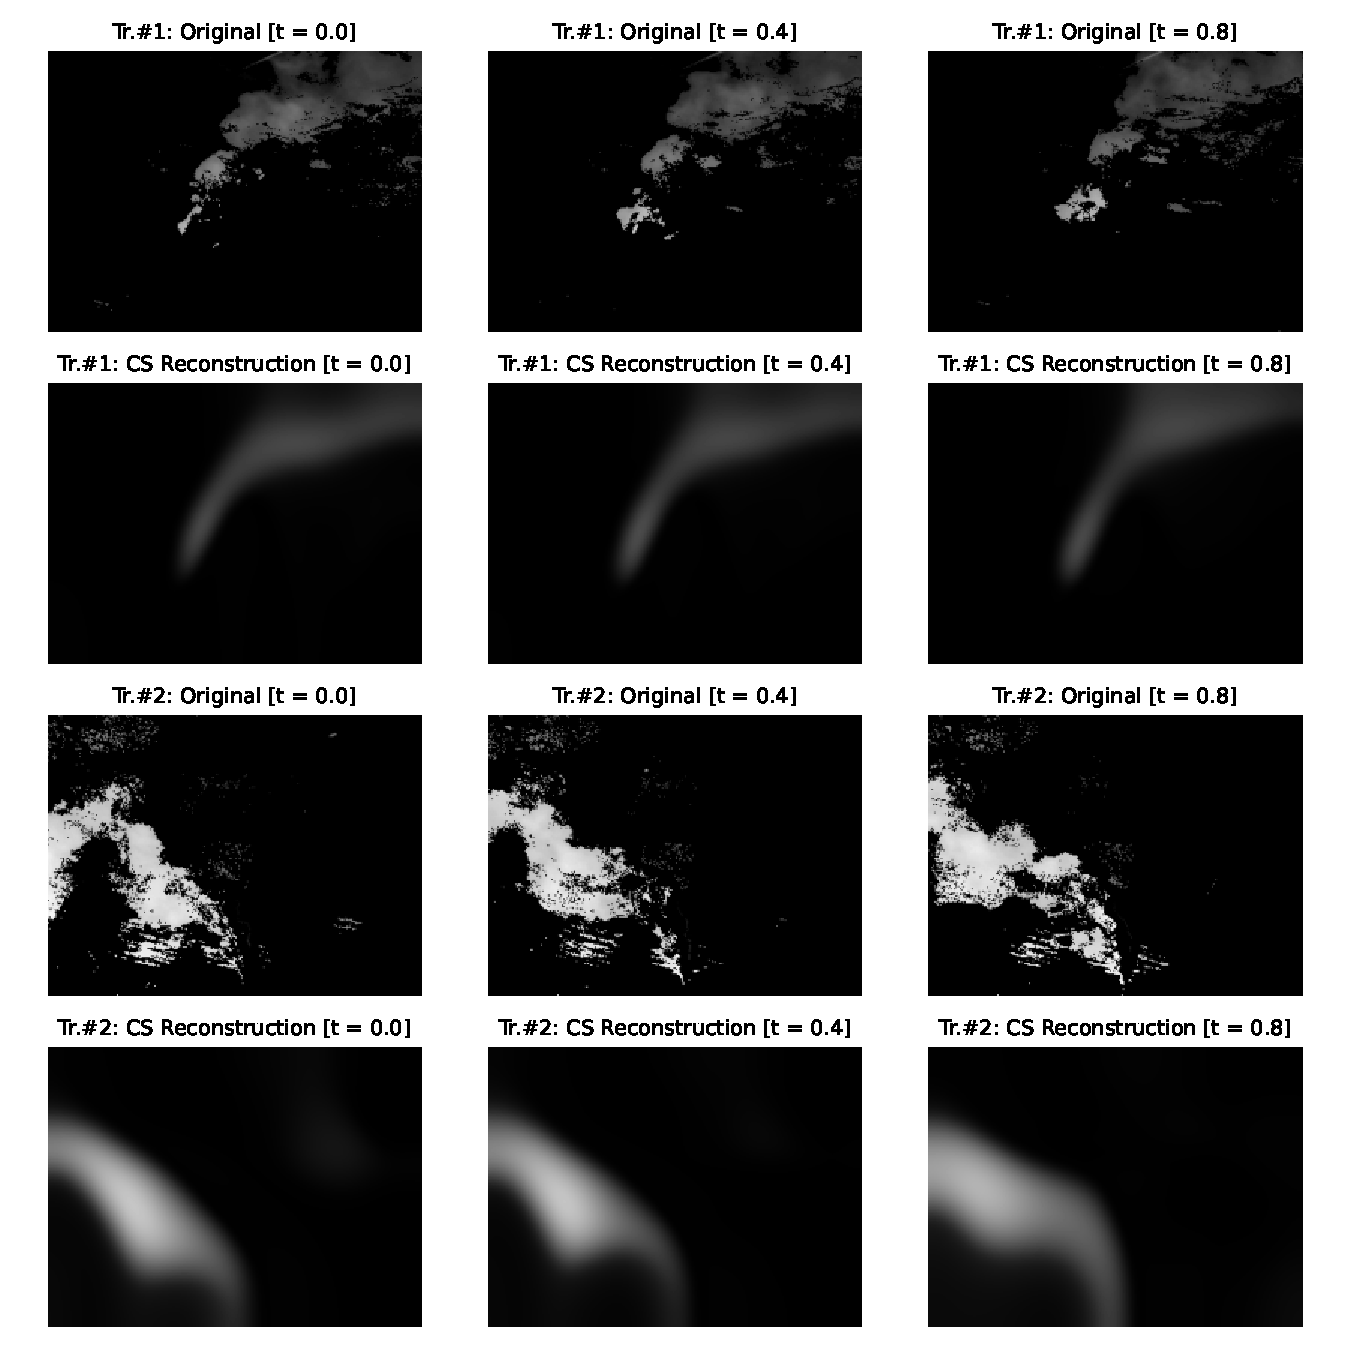
\includegraphics[width=\textwidth]{figures/cs_gas_examples.pdf}
	\caption{\label{fig:cs_gas_examples}}
\end{figure}

The example reconstructions are presented on Figure~\ref{fig:cs_gas_examples}. We see that the algorithm was able to faithfully reconstruct the trajectories. Although it was unable to capture the details of turbulent flows, it was able to predict the altitude, the direction, and the spread of the plumes correctly, which are the most important aspects for practical applications in real-world gas monitoring applications. 

We note the threefold difficulty of the task. First, the background subtraction struggles to separate grey smoke from a dynamic grey background, which leads to fantom clouds of smoke in processed data. Second, the amount of training data (3900 frames) is extremely small for training a large convolutional ROM. For example, \cite{wang2020machine} used the same dataset for training a simpler classification network (leak/non-leak) using ~11000 frames. Finally, an SPF of 0.66\% is vastly insufficient for frame-by-frame reconstruction, as most state-of-the-art methods require ~5-10\% SPF, depending on the nature of the picture (	\cite{wang2022single}). Thus, the inductive bias of the ROM becomes a crucial component for a successful video reconstruction.


\subsection{Discussion} 
In this work, we demonstrated how a collocation-point-based technique can improve the performance of an emerging class of continuous-time physics-informed neural-network-based reduced-order models. First, we demonstrated that the incorporation of collocation points in training data can ``cover the gaps'' in training trajectories and inform the model about underrepresented basins of attraction. Such an approach alleviates the demand for large volumes of data that is common in network-based models. Reducing the amount of data required to faithfully reconstruct a signal is extremely valuable in applications where data is scarce and expensive. Second, the physics-informed loss may work as a safeguard, providing a noise-free source of underlying dynamics.
Third, collocation points can stabilize the model's long-term predictions, allowing for accurate forecasting far beyond the training time horizon. Finally, together with using neural-ODE-based nonlinear latent dynamics, adding physics-informed loss leads to the discovery of more compact latent space representations that also yield more accurate models. Simultaneous stability and compactness is especially important if one aims to use models with compressive sensing and control algorithms. With respect to the computational complexity, we note that adding $Tk$ collocation points to the training imposes less of a computational burden than adding $k$ data trajectories, because, unlike data trajectories, collocation points do not require computing integrals forward in time. The last section served to illustrate how PINODE models that were developed in Section~\ref{sec:method} can help in applied modeling. In particular, we showed how one can employ a PINODE model for compressive-sensing purposes. We illustrated its performance on two examples: Burger's equation and Kolmogorov flow. In these cases, it is clear that PINODE can serve as a powerful regularizer and allow users to go significantly below the limits of the Nyquist sampling theorem. 

One clear limitation of the current work is that the choice of an efficient collocation family is a design decision that a practitioner makes. We believe that such decisions can be automated by adopting existing approaches from classic works on numerical approximations of PDEs, which we leave for future research. Another automation that prompts future research is deriving efficient ways of sampling collocation points, possibly via applying modern adaptive learning techniques \cite{subramanian2022adaptive}. Finally, although Section~\ref{sec:burger_noise} provides some rationale for why one may expect robustness of hybrid models under noise, we believe that a more rigorous analysis is possible, particularly one that provides conditions under which such robustness is guaranteed. 


\bibliographystyle{apalike}
\bibliography{bibliography}

\clearpage

\appendix
\chapter{Appendix}
\section{Acknowledgement}
I would like to thank my research advisors -- Dr. Aleksandr Aravkin, and Dr. Nathan Kutz, for their excellent leadership, continuous mentorship, and support in my journey as a Ph.D. student. I would also like to thank my collaborators -- Dr. James V. Burke, and Dr. Steven Brunton for their outstanding contributions to this work. I am grateful to Dr. Hassan Mansour and Dr. Saleh Nabi -- my colleagues and collaborators from Mitsubishi Electrics Research Labs who guided me to success throughout my internship in Spring 2023 and beyond. I wholeheartedly thank Biraj Pandey, Ryan Vogt, and Natalie Wellen -- my fellow Ph.D. students and dear friends from the Department of Applied Mathematics at UW: you turned what could have been a daunting and isolating journey into a wonderful experience full of happy memories. And even more so I would like to thank my family: my mom Svetlana Sholokhova, my grandmother Raisa Zakirova, and my wife Alanna Sholokhova. You have been surrounding me with unbelievable amounts of support and love, from close and afar, and I would have never succeeded in this journey without you. 

\section{Derivatives of Marginalized Log-likelihood for Linear Mixed Models}
\label{appendix:derivatives_of_lmm}
For conciseness, let us define the mismatch $\xi_i = Y_i - X_i\beta$. We also omit the dependence on $\beta$, as it's fixed at this point. The loss function \ref{eq:lmm_objective} takes the form 
\eq{
	\label{eq:lmm_simplified_gamma}
	\LL\pa{\gamma} = \sum_{i = 1}^m\half\xi_i^T\pa{\Omega_i(\gamma)}^{-1}\xi_i + \half\log\det\pa{\Omega_i(\gamma)}.
}

The derivative of the objective w.r.t $\gamma_j$, the $j$'th diagonal element of the matrix $\Gamma$ is

\eq{
	\pderiv{\xi_i^T\Omega_i^{-1}\xi_i}{\Gamma_{jj}} & = \trace \left[\left(\pderiv{\xi_i^T\Omega_i^{-1}\xi_i}{\Omega_i}\right)\pderiv{\Omega}{\Gamma_{jj}}\right] = \trace\left[\left(-\Omega_i^{-T}\xi_i\xi_i^T\Omega_i^{-T}\right)^T Z_i\pderiv{\Gamma}{\Gamma_{jj}}Z_i^T\right] =  
}

where $\pderiv{\Gamma}{\Gamma_{jj}}$ is a structure matrix, which, in a general case, is equal to a single-entry matrix $J^{jj}$ with $jj$'th element is equal to 1 and zeroes elsewhere. Substituting this back we get
\eq{
	= \trace\left[\left(-\Omega_i^{-T}\xi_i\xi_i^T\Omega_i^{-T}\right)^T Z^j_i{Z^j_i}^T\right] = 
} 
where $Z^j_i$ is a $j$'th column of the matrix $Z_i$. Making a circular swap we end up with

\eq{
	= \trace\left[-{Z^j_i}^T\Omega_i^{-T}\xi_i\xi_i^T\Omega_i^{-T} Z^j_i\right] = - ({Z_i^j}^T\Omega_i^{-T}\xi_i)^2
} 

Similarly,

\eq{
	\pderiv{\log\det\Omega_i}{\Gamma_{jj}} = \trace\left[\left(\pderiv{\log\det\Omega_i}{\Omega_i}\right)\pderiv{\Omega_i}{\Gamma_{jj}}\right] = \trace\left[\Omega_i^{-1}Z_i^j{Z_i^j}^T\right] = {Z_i^j}^T\Omega_i^{-1}Z_i^j
}

Taking into account that $\Omega_i$ is symmetric, we have 

\eq{
	\left[\nabla_\gamma \LL\pa{\beta, \gamma}\right]_j = \sum_{i = 1}^m  - ({Z_i^j}^T\Omega_i^{-T}\xi_i)^2 + {Z_i^j}^T\Omega_i^{-1}Z_i^j = 
}

or, in vector form

\eq{
    = \sum_{i = 1}^m  \diag{{Z_i}^T\Omega_i^{-1}Z_i} - ({Z_i}^T\Omega_i^{-T}\xi_i)^{\circ 2} =
}

where $\circ$ denotes the Hadamard (element-wise) product. Using the Cholesky decomposition $\Omega_i = L_iL_i^T$ we can calculate it more effectively, using only one triangular matrix inversion:

\eq{
    = \sum_{i = 1}^m \left[ \sum_{\text{rows}}\left(L_i^{-1}Z_i\right)^{\circ 2} -  [(L_i^{-1}Z_i)^{T}(L_i^{-1}\xi_i)]^{\circ 2}\right]
}

Notice, that the loss function (\ref{eq:lmm_objective}) and the optimal $\beta$ solution (\ref{eq:beta_formula}) can also be effectively computed using Cholesky:

\eq{
	\LL\pa{\gamma} = \sum_{i = 1}^m \half\xi_i^T\pa{\Omega_i(\gamma)}^{-1}\xi_i + \half\log\det\pa{\Omega_i(\gamma)} = \sum_{i = 1}^m \half\ \|L_i^{-1}\xi_i\|^2 - \sum_{j = 1}^k \log{[L^{-1}_i]}_{jj}
}

\eq{
	\beta_{k+1} & = \argmin_{\beta}\LL(\beta, \gamma_{k}) = \left(\sum_{i = 1}^m X_i^T\Omega_i^{-1}X_i\right)^{-1}\sum_{i = 1}^mX_i^T\Omega_i^{-1}y_i = \\
	& = \left(\sum_{i = 1}^m (L_i^{-1}X_i)^TL_i^{-1}X_i\right)^{-1}\sum_{i = 1}^m (L_i^{-1}X_i)^TL_i^{-1}y_i 
}




The Hessian w.r.t. $\gamma$ also can be found:

\eq{
	\frac{\partial^2 \LL\pa{\beta, \gamma}}{\partial \gamma_j^2} & = \sum_{i=1}^m -2({Z_i^j}^T\Omega_i^{-T}\xi_i)\trace\left[\frac{\partial{Z_i^j}^T\Omega_i^{-T}\xi_i}{\partial \Omega_i}\frac{\partial \Omega_i}{\partial \Gamma_{jj}} \right] + \trace\left[\frac{\partial{Z_i^j}^T\Omega_i^{-1}Z_i^j}{\partial \Omega_i}\frac{\partial \Omega_i}{\partial \Gamma_{jj}} \right] = \\
	& = \sum_{i=1}^m 2({Z_i^j}^T\Omega_i^{-T}\xi_i)\trace\left[\Omega_i^{-1}Z_i^j{\xi_i}^T\Omega_i^{-1}Z_i^j{Z_i^j}^T \right] - ({Z_i^j}^T\Omega_i^{-T}Z_i^j)^2 = \\
	& = \sum_{i=1}^m 2({Z_i^j}^T\Omega_i^{-T}\xi_i)({Z_i^j}^T\Omega_i^{-1}Z_i^j)({\xi_i}^T\Omega_i^{-1}Z_i^j) - ({Z_i^j}^T\Omega_i^{-T}Z_i^j)^2
}

\eq{
	\frac{\partial^2 \LL\pa{\beta, \gamma}}{\partial \gamma_j\partial \gamma_k} & = \sum_{i=1}^m -2({Z_i^j}^T\Omega_i^{-T}\xi_i)\trace\left[\frac{\partial{Z_i^j}^T\Omega_i^{-T}\xi_i}{\partial \Omega_i}\frac{\partial \Omega_i}{\partial \Gamma_{kk}} \right] + \trace\left[\frac{\partial{Z_i^j}^T\Omega_i^{-1}Z_i^j}{\partial \Omega_i}\frac{\partial \Omega_i}{\partial \Gamma_{kk}} \right] = \\
	& = \sum_{i=1}^m 2({Z_i^j}^T\Omega_i^{-T}\xi_i)\trace\left[\Omega_i^{-1}Z_i^j{\xi_i}^T\Omega_i^{-1}Z_i^k{Z_i^k}^T \right] - ({Z_i^j}^T\Omega_i^{-T}Z_i^k)^2 = \\
	& = \sum_{i=1}^m 2(\xi_i^T\Omega_i^{-T}{Z_i^j})({Z_i^j}^T\Omega_i^{-1}Z_i^k)({Z_i^k}^T\Omega_i^{-1}{\xi_i}) - ({Z_i^j}^T\Omega_i^{-T}Z_i^k)^2
}

\eq{
	\label{eq:lmm_hessian_gamma}
	\nabla^2_\gamma\LL\pa{\beta, \gamma} = \half\sum_{i = 1}^m -(Z_i^T\Omega_i^{-T}Z_i)^{\circ 2}  + 2\diag(Z_i^T\Omega_i^{-T}\xi_i)(Z_i^T\Omega^{-1}Z_i)\diag(\xi_i^T\Omega^{-T}Z_i) = \\
	= \half\sum_{i = 1}^m -(Z_i^T\Omega_i^{-T}Z_i)^{\circ 2} + 2(Z_i^T\Omega_i^{-T}\xi_i)(\xi_i^T\Omega^{-T}Z_i)^T\circ(Z_i^T\Omega^{-1}Z_i)
}



\section{Description of Datasets}
\subsection{GBD Bullying Data}
\label{appendix:bullying_covariates}
The author acknowledges his colleague and collaborator Damian Santomauro\footnote{\href{mailto:d.santomauro@uq.edu.au}{d.santomauro@uq.edu.au}, Affiliate Assistant Professor of Health Metrics Sciences, Institute for Health Metrics and Evaluation, University of Washington} for providing the dataset, the description of its covariates, and the expert assessment of their historical importance in different rounds of GBD study below.
\begin{enumerate}
	\item \texttt{cv\_symptoms}
	\begin{itemize}
		\item 0 = study assesses participants for MDD or anxiety disorders via a diagnostic interview to determine whether they have a diagnosis. 
		\item 1 = study uses a symptom scale (e.g., Beck Depression Inventory) and uses an established cut-off on that scale to determine caseness. 
		\item Has not historically been significant. 
	\end{itemize}
	\item \texttt{cv\_unadjusted}
	\begin{itemize}
		\item 0 = RR is adjusted for potential confounders (e.g., SES, etc.)	
		\item 1 = RR is not adjusted for potential confounders
		\item Has been significant in the past.
	\end{itemize}
	\item \texttt{cv\_b\_parent\_only} 
	\begin{itemize}
		\item 0 = Child is involved in reporting their own exposure to bullying.
		\item 1 = Only parent is involved in reporting the child’s exposure to bullying
		\item This covariate has recently started becoming significant (but not consistently). 
	\end{itemize}
	\item \texttt{cv\_or}
	\begin{itemize}
		\item 0 = estimate is a RR
		\item 1 = estimate is an odds ratio (OR)
		\item ORs are always larger than RRs. However the magnitude may be very small / insignificant.
	\end{itemize}
	\item \texttt{cv\_multi\_reg}
	\begin{itemize}
		\item 0 = RR is the ratio of the rate of the outcome in persons exposed vs all persons unexposed (including persons exposed to low-threshold bullying victimization)
		\item 1 =  RRs are estimated via a logistic regression where exposure represented by 3 categories: 1) No exposure, 2) Occasional exposure, 3) Frequent exposure. The RR for occasional exposure will exclude participants with frequent exposure, and the RR for frequent exposure will exclude participants with occasional exposure. 
		\item Is expected to be significant.
	\end{itemize}
	\item \texttt{cv\_low\_threshold\_bullying}
	\begin{itemize}
		\item 0 = uses a ‘frequent’ exposure frequency threshold for classing someone as exposed to bullying.
		\item 1 = uses an ‘occasional’ exposure frequency threshold for classing someone as exposed to bullying.
		\item Has been consistently significant with a strong magnitude.
	\end{itemize}
	\item \texttt{cv\_anx}
	\begin{itemize}
		\item 0 = estimate represents risk for MDD
		\item 1 = estimate represents risk for anxiety disorders
	\end{itemize}
	\item \texttt{cv\_selection\_bias}
	\begin{itemize}
		\item 0 = < 15\% attrition at followup
		\item 1 = $\geqslant$ 15\% attrition at followup
		\item Has been significant in the past
	\end{itemize}
	\item \texttt{Percent\_female}
	\begin{itemize}
		\item Indicates \% of sample in estimate that are female. 
	\end{itemize}
	\item \texttt{cv\_child\_baseline}
	\begin{itemize}
		\item Has not been significant in the past.
	\end{itemize}
\end{enumerate}


\subsection{COVID-19 Contact Rate Forecasting Data}
\begin{longtable}{llll}
\caption{List of locations, number of observations, start and end date for each location for COVID-19 Contact Rate Forecasting data}\\
\toprule
                   Location & Obs &      Start &        End \\
\midrule
\endhead
\midrule
\multicolumn{4}{r}{{Continued on next page}} \\
\midrule
\endfoot

\bottomrule
\endlastfoot
                   Malaysia &  60 & 2020-02-27 & 2020-04-26 \\
                Philippines &  67 & 2020-02-21 & 2020-04-27 \\
                   Bulgaria &  50 & 2020-03-09 & 2020-04-27 \\
                    Croatia &  50 & 2020-03-08 & 2020-04-26 \\
                    Czechia &  54 & 2020-03-05 & 2020-04-27 \\
                    Hungary &  55 & 2020-03-04 & 2020-04-27 \\
                     Poland &  56 & 2020-03-03 & 2020-04-27 \\
                    Romania &  56 & 2020-03-03 & 2020-04-27 \\
                     Serbia &  55 & 2020-03-04 & 2020-04-27 \\
                   Slovakia &  32 & 2020-03-26 & 2020-04-26 \\
                   Slovenia &  54 & 2020-03-05 & 2020-04-27 \\
                    Estonia &  48 & 2020-03-10 & 2020-04-26 \\
                     Latvia &  26 & 2020-04-01 & 2020-04-26 \\
                  Lithuania &  53 & 2020-03-05 & 2020-04-26 \\
        Republic of Moldova &  48 & 2020-03-11 & 2020-04-27 \\
                    Ukraine &  53 & 2020-03-06 & 2020-04-27 \\
                      Japan &  68 & 2020-02-20 & 2020-04-27 \\
          Republic of Korea &  85 & 2020-02-02 & 2020-04-26 \\
                    Austria &  62 & 2020-02-26 & 2020-04-27 \\
                    Belgium &  65 & 2020-02-23 & 2020-04-27 \\
                     Cyprus &  49 & 2020-03-09 & 2020-04-26 \\
                    Denmark &  61 & 2020-02-27 & 2020-04-27 \\
                    Finland &  53 & 2020-03-06 & 2020-04-27 \\
                     France &  63 & 2020-02-24 & 2020-04-26 \\
                     Greece &  62 & 2020-02-26 & 2020-04-27 \\
                    Iceland &  43 & 2020-03-15 & 2020-04-26 \\
                    Ireland &  58 & 2020-03-01 & 2020-04-27 \\
                     Israel &  56 & 2020-03-03 & 2020-04-27 \\
                 Luxembourg &  58 & 2020-02-29 & 2020-04-26 \\
                Netherlands &  61 & 2020-02-27 & 2020-04-27 \\
                     Norway &  62 & 2020-02-26 & 2020-04-27 \\
                   Portugal &  58 & 2020-03-01 & 2020-04-27 \\
                     Sweden &  63 & 2020-02-25 & 2020-04-27 \\
                Switzerland &  69 & 2020-02-19 & 2020-04-27 \\
             United Kingdom &  70 & 2020-02-18 & 2020-04-27 \\
                  Argentina &  56 & 2020-03-03 & 2020-04-27 \\
                      Chile &  54 & 2020-03-05 & 2020-04-27 \\
         Dominican Republic &  58 & 2020-03-01 & 2020-04-27 \\
                    Ecuador &  50 & 2020-03-01 & 2020-04-19 \\
                       Peru &  55 & 2020-03-04 & 2020-04-27 \\
                   Colombia &  55 & 2020-03-04 & 2020-04-27 \\
                     Panama &  50 & 2020-03-09 & 2020-04-27 \\
                      Egypt &  68 & 2020-02-20 & 2020-04-27 \\
 Iran (Islamic Republic of) &  69 & 2020-02-19 & 2020-04-27 \\
                     Turkey &  48 & 2020-03-11 & 2020-04-27 \\
                Puerto Rico &  45 & 2020-03-14 & 2020-04-27 \\
                    Alabama &  48 & 2020-03-11 & 2020-04-27 \\
                     Alaska &  49 & 2020-03-09 & 2020-04-26 \\
                    Arizona &  55 & 2020-03-04 & 2020-04-27 \\
                   Arkansas &  52 & 2020-03-07 & 2020-04-27 \\
                 California &  67 & 2020-02-21 & 2020-04-27 \\
                   Colorado &  54 & 2020-03-05 & 2020-04-27 \\
                Connecticut &  52 & 2020-03-07 & 2020-04-27 \\
                   Delaware &  51 & 2020-03-08 & 2020-04-27 \\
       District of Columbia &  54 & 2020-03-05 & 2020-04-27 \\
                    Florida &  57 & 2020-03-02 & 2020-04-27 \\
                    Georgia &  56 & 2020-03-03 & 2020-04-27 \\
                     Hawaii &  43 & 2020-03-15 & 2020-04-26 \\
                      Idaho &  50 & 2020-03-08 & 2020-04-26 \\
                   Illinois &  55 & 2020-03-04 & 2020-04-27 \\
\end{longtable}

\begin{longtable}{lrrrrr}
\caption{List of location-specific coefficients for the R\&S-Mixed model fit,  as well as RMSEs for three models discussed in the respective chapterCoefficient for \texttt{temperature} was set to -674.86. Coefficients for \texttt{proportion\_over\_1k} and \texttt{testing\_reference} were set to 0.}\label{table:covid_coefficients}\\
\toprule
                   Location &  Intercept &  Mobility &  RMSE\_IHME &  RMSE\_Dense &  RMSE\_Sparse \\
\midrule
\endhead
\midrule
\multicolumn{6}{r}{{Continued on next page}} \\
\midrule
\endfoot

\bottomrule
\endlastfoot
                   Malaysia &      13.94 &     52.15 &       5.17 &        5.00 &         5.00 \\
                Philippines &      13.60 &     29.45 &       4.20 &        4.16 &         4.16 \\
                   Bulgaria &      14.24 &    123.94 &       3.42 &        3.20 &         3.20 \\
                    Croatia &      13.28 &     56.84 &       3.70 &        3.67 &         3.67 \\
                    Czechia &      13.77 &    103.24 &       2.86 &        3.07 &         3.12 \\
                    Hungary &      12.51 &     28.59 &       0.73 &        0.70 &         0.72 \\
                     Poland &      12.66 &     39.47 &       0.64 &        0.58 &         0.62 \\
                    Romania &      13.63 &     80.40 &       3.59 &        3.89 &         4.01 \\
                     Serbia &      13.16 &     56.92 &       3.79 &        3.80 &         3.84 \\
                   Slovakia &      11.27 &    -43.53 &       5.27 &        4.50 &         5.01 \\
                   Slovenia &      12.74 &     42.75 &       1.46 &        1.40 &         1.56 \\
                    Estonia &      14.17 &    155.26 &       2.21 &        2.55 &         2.73 \\
                     Latvia &      11.82 &    -14.61 &       4.94 &        4.41 &         4.68 \\
                  Lithuania &      12.96 &     66.04 &       3.89 &        3.86 &         3.86 \\
        Republic of Moldova &      15.15 &    153.32 &       3.05 &        2.44 &         2.44 \\
                    Ukraine &      13.54 &    103.82 &       3.06 &        3.29 &         3.30 \\
                      Japan &      12.47 &     35.51 &       4.21 &        4.22 &         4.22 \\
          Republic of Korea &      12.62 &     99.62 &       4.84 &        4.67 &         4.70 \\
                    Austria &      13.07 &     64.96 &       3.97 &        3.90 &         3.93 \\
                    Belgium &      13.44 &     51.77 &       3.47 &        3.39 &         3.39 \\
                     Cyprus &      12.65 &     25.21 &       1.84 &        0.64 &         0.66 \\
                    Denmark &      12.79 &     47.14 &       1.79 &        1.87 &         1.94 \\
                    Finland &      12.87 &     73.08 &       3.53 &        3.63 &         3.68 \\
                     France &      12.95 &     32.79 &       1.57 &        1.64 &         1.66 \\
                     Greece &      12.74 &     29.97 &       1.42 &        1.56 &         1.56 \\
                    Iceland &      16.35 &    226.87 &       5.77 &        3.09 &         3.17 \\
                    Ireland &      13.54 &     57.98 &       3.98 &        4.00 &         4.00 \\
                     Israel &      13.83 &     66.97 &       3.46 &        3.71 &         3.71 \\
                 Luxembourg &      12.51 &     21.39 &       1.47 &        1.53 &         1.73 \\
                Netherlands &      12.90 &     52.99 &       1.35 &        1.46 &         1.47 \\
                     Norway &      12.22 &     34.27 &       1.70 &        1.64 &         1.65 \\
                   Portugal &      13.51 &     52.51 &       2.47 &        2.55 &         2.55 \\
                     Sweden &      12.95 &     99.37 &       3.93 &        3.80 &         3.90 \\
                Switzerland &      12.68 &     66.51 &       3.79 &        3.88 &         3.98 \\
             United Kingdom &      13.28 &     51.22 &       4.70 &        4.71 &         4.72 \\
                  Argentina &      13.29 &     36.93 &       1.45 &        1.63 &         1.67 \\
                      Chile &      13.64 &     73.48 &       3.51 &        3.62 &         3.63 \\
         Dominican Republic &      13.78 &     40.14 &       2.21 &        2.23 &         2.23 \\
                    Ecuador &      15.97 &    128.02 &       8.21 &        8.07 &         8.07 \\
                       Peru &      12.97 &     16.00 &       1.08 &        0.96 &         1.18 \\
                   Colombia &      13.88 &     47.20 &       3.63 &        3.63 &         3.63 \\
                     Panama &      13.12 &     10.67 &       0.25 &        0.27 &         0.27 \\
                      Egypt &      13.11 &     41.80 &       3.89 &        3.95 &         3.96 \\
 Iran (Islamic Republic of) &      12.27 &     15.23 &       0.93 &        1.03 &         1.05 \\
                     Turkey &      12.60 &     28.83 &       0.27 &        0.18 &         0.17 \\
                Puerto Rico &      13.76 &     45.18 &       0.68 &        0.34 &         0.35 \\
                    Alabama &      12.81 &     27.02 &       0.70 &        0.65 &         0.84 \\
                     Alaska &      12.24 &     57.82 &       3.85 &        3.98 &         4.00 \\
                    Arizona &      13.40 &     66.31 &       4.00 &        3.85 &         4.03 \\
                   Arkansas &      13.32 &     91.92 &       4.02 &        3.87 &         3.88 \\
                 California &      13.14 &     54.89 &       3.81 &        3.86 &         3.88 \\
                   Colorado &      12.45 &     37.13 &       0.75 &        1.01 &         1.03 \\
                Connecticut &      13.28 &     69.51 &       0.59 &        0.77 &         0.92 \\
                   Delaware &      13.34 &     68.28 &       3.86 &        3.77 &         3.83 \\
       District of Columbia &      13.27 &     49.45 &       3.42 &        3.55 &         3.56 \\
                    Florida &      13.34 &     30.01 &       0.29 &        0.34 &         0.36 \\
                    Georgia &      12.74 &     19.19 &       0.45 &        0.34 &         0.66 \\
                     Hawaii &      14.97 &    134.74 &       3.74 &        3.34 &         3.39 \\
                      Idaho &      12.75 &     92.74 &       3.81 &        3.84 &         3.89 \\
                   Illinois &      12.73 &     32.57 &       0.64 &        0.56 &         0.70 \\
\end{longtable}


\end{document}
